% !Mode:: "TeX:UTF-8"
% chktex-file 19
% chktex-file 46
% 模板文档:https://github.com/jinyiliu/bnu-thesis-template

% 
% 编译说明
%		使用 XeLaTeX 编译引擎
%       TeX Live 的版本 2022 和 2021 目前都可以成功编译
%       如果使用 Overleaf 进行写作,请在左上角菜单中选择编译器为 XeLaTeX
%		在 MacBook 中推荐使用编译软件 Texpad


\documentclass[doctor]{bnuthesis}
	% bachelor/master/doctor: 学士/硕士/博士学位论文
	% twoside: 奇数页和偶数页页边距不一样,用于打印
	\usepackage{bnutils}
	% 调用宏包,使用 GB/T 7714-2015 参考文献著录格式
	\usepackage{gbt7714}
	% 这三条命令使用自动调整宽度的表格
	% https://zhuanlan.zhihu.com/p/542672514
	\usepackage{tabularx} % for 'tabularx' env. and 'X' col. type
	\usepackage{ragged2e} % for \RaggedRight macro
	\usepackage{booktabs} % for \toprule, \midrule etc macros
	%% create a derivative column type called 'L':
	\usepackage{pdflscape}  % 横过来页面,参考https://weibo.com/5342622960/GifjJhxIK
	\usepackage{rotating}  % 旋转表格,参考https://weibo.com/5342622960/GifjJhxIK
	\usepackage{adjustbox}  % 旋转 box,参考https://www.latex4technics.com/?note=1OI3
	\newcolumntype{L}{>{\RaggedRight\hangafter=1\hangindent=0em}X}

	\begin{document}
	\graphicspath{{img/}}
	
	\frontmatter
	% !Mode:: "TeX:UTF-8"

\ctitle{流域治理视角下黄河人-水关系演变过程及驱动机制}
\etitle{Co-evolution of human-water interactions from a governing perspective in the Yellow River Basin, China: processes and mechanism}


\makeatother

% 学士学位封面
% \cbuyuanxi{天文系} % 部院系
% \czhuanye{天文学} % 专业
% \cxuehao{201511160109} % 学号
% \cxueshengxingming{某某某} % 学生姓名
% \czhidaojiaoshi{某某} % 指导教师
% \czhidaojiaoshizhicheng{教授} % 指导教师职称
% \czhidaojiaoshidanwei{北京师范大学天文系} % 指导教师单位

% 博士(硕士)学位封面
\czuozhe{宋爽} % 作者
\cdaoshi{傅伯杰\ 教授} % 导师
\cxibienianji{地理学部2018级} % 系别年级
\cxuehao{201831051016} % 学号
\cxuekezhuanye{自然地理} % 学科专业
\cwanchengriqi{2023年4月} % 完成日期


\begin{cabstract}
% 论文的摘要是对论文研究内容和成果的高度概括。摘要应对论文所研究的问题及其研究目的进行描述,对研究方法和过程进行简单介绍,对研究成果和所得结论进行概括。摘要应具有独立性和自明性,其内容应包含与论文全文同等量的主要信息。使读者即使不阅读全文,通过摘要就能了解论文的总体内容和主要成果。

% 论文摘要的书写应力求精确、简明。切忌写成对论文书写内容进行提要的形式,尤其要避免“第 1 章……;第 2 章……;……”这种或类似的陈述方式。

% 本文介绍北京师范大学论文模板 BNUThesis 的使用方法。本模板是在清华大学学位论文模板 THUThesis 的基础上修改而来,以及BNU硕博士模板BNUThesis上修改完成。完全参照《毕业论文写作规范(修订)》(师教文[2007]186 号)、北京师范大学图书馆Word版学士模板、北京师范大学信息科学与技术学院Word版写作模板的格式要求制作而成。

大河流域是人类起源和发展的中心,随着人类活动改变了流域的自然和社会水循环过程,许多大河流域出现了不可持续的发展态势。
治理黄河是中华民族的千年夙愿,重塑黄河人水关系、实现黄河流域生态保护和高质量发展也是国家的重大战略。
因此,研究黄河流域人水关系演变规律、揭示演变机制,可为黄河流域治理提供理论基础和科学依据。
本研究结合水文气象观测、社会经济统计、历史数据重建和遥感反演等多源数据,借助统计分析、因果推断、与多主体建模等手段,发展了流域人水关系演变的识别与分析框架及机制分析方法,在历史时期和现代治黄时期定量划分黄河流域人水关系演变的主要阶段与过程、识别了推动人水关系变化的关键机制,主要研究结论如下:

(1)历史时期黄河流域存水沙变化的在两个湿润气候驱动期($900AD\sim1100AD$和$1700AD\sim1900AD$)和两个人类活动驱动期($1350AD \sim 1650AD$ 和 $1900AD$迄今)。其中第一个气候驱动期位于“中世纪暖期”(约$900AD \sim 1100AD$),此时黄河的水沙变化变化仍由气候因素主导。随后中游黄土高原地区发生农田与人口的快速扩张,不断增加的人为压力与另一次潮湿气候共同推动水沙特征在$1700AD \sim 1900AD$越过变化的临界点。上述结果表明人类活动带来的影响最早追溯至$1350AD$才开始取代周期变化的气候,逐步成为历史时期主导黄河流域人-水关系的主要因素。

(2)本研究使用综合水治理指数(IWGI)将当代治黄时期的流域水治理演变过程划分为三个阶段,并依据其各自特点命名为:集中供水时期($1965 \sim 1978$年)、治理转变时期($1979 \sim 2001$年)、以及适应增强时期($2002 \sim 2013$年)。灌区扩张和水库修建的放缓,是黄河从集中供水时期向治理转变时期过渡的主要特征。在治理转变时期流域的非工程治理措施迅速增加,过渡至适应增强时期后保持稳定,并着重提升用水效率。经讨论,上述治理模式转变可能在全世界流域系统中普遍存在,而本研究的分析指出水资源供给趋近极限可能是触发转变的关键。

(3)在上述治理转变期,$1987$年提出的黄河水资源配额制度及其在$1998$年的改革,是对流域影响深远的典型非工程治理政策。本研究指出这两次制度变化以不同的方式重塑了黄河流域的社会-生态系统结构,因而较政策初衷而言产生了不同的治理效果。其中,$1987$年通过的“八七”分水方案违背制度预期地使黄河流域用水量显著增加约$5.75\%$;而$1998$年参照该分水方案施行流域统一调度之后,大多数省份地区的用水量迅速得到控制,流域总用水在接下来十年间以每年$6.6$亿立方米的速度显著下降,成功治理了长达二十余年的黄河断流问题。

(4)黄河水资源配额制度在$1987$年与$1998$年两次变化对流域用水产生的影响,是用水者主体自下而上响应并适应制度变化的表现。本研究耦合了反映水资源配额制度的人类社会模块与计算三种主要粮食作物(水稻、玉米、小麦)灌溉用水需求的自然模块,发展了黄河流域农业灌溉用水者响应分水制度变化的多主体模型。模型仿真结果表明黄河流域的粮食生产灌溉需求与水资源配额之间存在时空不匹配,配额在$1987$至$1998$年间对用水的约束效果不明显,而$1998$年之后,配额制度在约束地表取水的同时也没有导致大规模的地下水开采。

本研究定量识别并划分了黄河流域人水关系演变过程的主要阶段、发展了分析其驱动机制的因果推断方法、开发了黄河流域社会-生态系统的多主体模型、自下而上解析了农业用水主体对制度变化的响应如何导致不同的流域治理效果。
本研究从流域系统治理和人水关系演变的视角为黄河流域的高质量、可持续发展提供科学基础和决策依据,重点解析了过去常常被忽视的流域非工程治理措施对人水关系演变的驱动作用,为流域治理制度的设计提供科学评估方法,这在世界大河流域非工程治理措施日益增多的当今显得尤为重要。

  % 本文的创新点主要有:
  % \begin{itemize}[$\bullet$]
  %   \item 用例子来解释模板的使用方法;
  %   \item 用废话来填充无关紧要的部分;
  %   \item 一边学习摸索一边编写新代码。
  % \end{itemize}

  % 关键词是为了文献标引工作、用以表示全文主要内容信息的单词或术语。关键词不超过5个,每个关键词中间用分号分隔。(模板作者注:关键词分隔符不用考虑,模板会自动处理。英文关键词同理。)
\end{cabstract}
\ckeywords{黄河流域, 人水关系, 稳态转换, 水治理, 多主体模型}



\begin{eabstract}
  Large river basins have been crucial to human society and its development. However, human activities have altered the natural and social water cycles in these basins, leading to unsustainable situation and unprecedented tension relationship between humans and rivers. Controlling the Yellow River has long been an aspiration of the Chinese nation, and a major national strategy aims to restore the human-water relationship in the Yellow River Basin, ensuring ecological protection and high-quality development.

  To facilitate this goal, it is vital to study the evolution of the human-water relationship in the Yellow River Basin and reveal its processes and underlying mechanisms. This will deepen our understanding of the regional human-earth interactions and provide a theoretical and scientific foundation for the governance of the Yellow River Basin. In this study we focus human-water interactions of the Yellow River Basin, China. We develop identification and analysis frameworks for the evolution of the human-water relationship by using statistical analysis and other methods, drawing upon multi-source data such as hydro-meteorological observations, socio-economic statistics, historical data reconstruction, and remote sensing. Our frameworks allow for quantitative divisions of the main stages and processes in the evolution of the human-water relationship in the Yellow River Basin during historical and modern periods.
  
  Furthermore, this study develops a causal inference method for analyzing the evolution mechanisms of the human-water relationship in the Yellow River Basin. A agent-based model of the socio-ecological system in the Yellow River Basin is established, and the key mechanisms driving the changes in the human-water relationship are identified. The main conclusions are as follows:

  (1) The historical period of the Yellow River Basin witnessed two wet climate-driven phases ($900 AD \sim 1100 AD$ and $1700 AD \sim 1900 AD$) and two human activity-driven phases ($1350 AD \sim 1650 AD$ and $1900 AD$ to present). The first climate-driven phase, also known as the Medieval Warm Period (approximately $900 AD \sim 1100 AD$), was dominated by climate-induced changes in the comprehensive index. Subsequently, rapid expansion of farmland and population on the Loess Plateau led to increasing human pressure, which, combined with a humid climate, drove water and sediment changes beyond a critical point during the second wet phase ($1700 AD \sim 1900 AD$). This suggests that human activity began to replace cyclical climate fluctuations as the primary driver of the human-water relationship in the Yellow River Basin after $1350 AD$.

  (2) In the contemporary period of Yellow River management, the water management evolution process can be divided into three stages: the centralized water supply period ($1965 \sim 1978$), the management transition period ($1979 \sim 2001$), and the adaptation enhancement period ($2002 \sim 2013$). Irrigation expansion and economic growth were the direct causes of changes in the first two stages. Environmental background, social culture, and water management policies had varying degrees of influence in each stage and were the main driving forces behind the transition from the second stage to the third stage. Such a management transition model is common in global river systems, with water resource supply approaching its limit as a potential key trigger for change.
  
  (3) The Yellow River Basin's surface water allocation system experienced two significant changes, which constituted far-reaching policy interventions during the management transition period. These interventions reshaped the social-ecological system structure of the Yellow River Basin and produced distinctly different management outcomes. The $1987$ water allocation plan unexpectedly led to an approximately $5.75\%$ increase in water usage in the Yellow River Basin. However, after the basin-wide unified scheduling in $1998$, water usage in most areas was quickly controlled, resulting in a significant annual decrease of $660$ million cubic meters in total water usage, effectively ending the Yellow River's over two-decade-long dry-up.
  
  (4) There was a spatial-temporal mismatch between the surface water quota stipulated by the water resources allocation system in the Yellow River Basin and the irrigation demand of three main food crops (rice, maize and wheat) in the basin. By developing a multi-agent model of responsive water allocation system for grain irrigation in the Yellow River Basin, we find that the water resource allocation system that restricts surface water intake does not directly lead to large-scale underground water substitute exploitation, and water-saving transformation is the main way to respond to system changes in each region.

  This study reveals the evolution process of human-water relationship in the Yellow River Basin, analyzes the main reasons driving the evolution of human-water relationship in different stages, develops a causal analysis method for the mechanism of human-water relationship change in the Yellow River Basin, establishes an agent-based model of the socio-ecological system in the Yellow River Basin, clarifies the mechanism of institution-driven human-water relationship change and evaluates its impact quantitatively. 
  From the perspective of river basin governance and human-water relationship evolution, this study provides scientific basis and decision-making basis for the high-quality and sustainable development of the Yellow River Basin. This study also provide innovative methods for the design of water governance and the analysis of institutional response mechanism, which is particularly important in today's world where attempts of non-engineering governance practices are growing.

\end{eabstract}
\ekeywords{Yellow River Basin, Human-water interactions, Regime shift, Water governance, Agent-based model}



	\makecover{}
	
	\tableofcontents
	\listoffigures % 插图索引
	\listoftables % 表格索引
		
	%%% 正文部分
	\mainmatter{}
	% % !Mode:: "TeX:UTF-8"

\chapter{带 English 的标题}
\label{cha:intro}

这是 \bnuthesis{} 的示例文档,基本上覆盖了模板中所有格式的设置。建议大家在使用模板之前,除了阅读《\bnuthesis{}用户手册》,这个示例文档也最好能看一看。

小老鼠偷吃热凉粉;短长虫环绕矮高粱。\footnote{韩愈(768-824),字退之,河南河阳(今河南孟县)人,自称郡望昌黎,世称韩昌黎。幼孤贫刻苦好学,德宗贞元八年进士。曾任监察御史,因上疏请免关中赋役,贬为阳山县令。后随宰相裴度平定淮西迁刑部侍郎,又因上表谏迎佛骨,贬潮州刺史。做过吏部侍郎,死谥文公,故世称韩吏部、韩文公。是唐代古文运动领袖,与柳宗元合称韩柳。诗力求险怪新奇,雄浑重气势。}


\section{封面相关}
封面的例子请参看 cover.tex。主要符号表参看 denation.tex,附录和个人简历分别参看 appendix01.tex 和 resume.tex。里面的命令都非常简单,一看即会。\footnote{你说还是看不懂?怎么会呢?}

\section{字体命令}
\label{sec:first}

苏轼(1037-1101),北宋文学家、书画家。字子瞻,号东坡居士,眉州眉山(今属四川)人。苏洵子。嘉佑进士。神宗时曾任祠部员外郎,因反对王安石新法而求外职,任杭州通判,知密州、徐州、湖州。后以作诗“谤讪朝廷”罪贬黄州。哲宗时任翰林学士,曾出知杭州、颖州等,官至礼部尚书。后又贬谪惠州、儋州。北还后第二年病死常州。南宋时追谥文忠。与父洵弟辙,合称“三苏”。在政治上属于旧党,但也有改革弊政的要求。其文汪洋恣肆,明白畅达,为“唐宋八大家”之一。  其诗清新豪健,善用夸张比喻,在艺术表现方面独具风格。少数诗篇也能反映民间疾苦,指责统治者的奢侈骄纵。词开豪放一派,对后代很有影响。《念奴娇·赤壁怀古》、《水调歌头·丙辰中秋》传诵甚广。

{\kai 坡仙擅长行书、楷书,取法李邕、徐浩、颜真卿、杨凝式,而能自创新意。用笔丰腴跌宕,有天真烂漫之趣。与蔡襄、黄庭坚、米芾并称“宋四家”。能画竹,学文同,也喜作枯木怪石。论画主张“神似”,认为“论画以形似,见与儿童邻”;高度评价“诗中有画,画中有诗”的艺术造诣。诗文有《东坡七集》等。存世书迹有《答谢民师论文帖》、《祭黄几道文》、《前赤壁赋》、《黄州寒食诗帖》等。  画迹有《枯木怪石图》、《竹石图》等。}

{\fs 易与天地准,故能弥纶天地之道。仰以观於天文,俯以察於地理,是故知幽明之故。原始反终,故知死生之说。精气为物,游魂为变,是故知鬼神之情状。与天地相似,故不违。知周乎万物,而道济天下,故不过。旁行而不流,乐天知命,故不忧。安土敦乎仁,故能爱。范围天地之化而不过,曲成万物而不遗,通乎昼夜之道而知,故神无方而易无体。}

{\you 有天地,然后万物生焉。盈天地之间者,唯万物,故受之以屯;屯者盈也,屯者物之始生也。物生必蒙,故受之以蒙;蒙者蒙也,物之穉也。物穉不可不养也,故受之以需;需者饮食之道也。饮食必有讼,故受之以讼。讼必有众起,故受之以师;师者众也。众必有所比,故受之以比;比者比也。比必有所畜也,故受之以小畜。物畜然后有礼,故受之以履。}

{\hei 履而泰,然后安,故受之以泰;泰者通也。物不可以终通,故受之以否。物不可以终否,故受之以同人。与人同者,物必归焉,故受之以大有。有大者不可以盈,故受之以谦。有大而能谦,必豫,故受之以豫。豫必有随,故受之以随。以喜随人者,必有事,故受之以蛊;蛊者事也。}

{\li 有事而后可大,故受之以临;临者大也。物大然后可观,故受之以观。可观而后有所合,故受之以噬嗑;嗑者合也。物不可以苟合而已,故受之以贲;贲者饰也。致饰然后亨,则尽矣,故受之以剥;剥者剥也。物不可以终尽,剥穷上反下,故受之以复。复则不妄矣,故受之以无妄。}

{\song 有无妄然后可畜,故受之以大畜。物畜然后可养,故受之以颐;颐者养也。不养则不可动,故受之以大过。物不可以终过,故受之以坎;坎者陷也。陷必有所丽,故受之以离;离者丽也。}

\section{表格样本}
\label{chap1:sample:table} 

\subsection{基本表格}
\label{sec:basictable}

模板中关于表格的宏包有三个: \textsf{booktabs}、\textsf{array} 和\textsf{longtabular},命令有一个 \verb|\hlinewd|。三线表可以用 \textsf{booktabs}提供的 \verb|\toprule|、\verb|\midrule| 和 \verb|\bottomrule|。它们与\textsf{longtable} 能很好的配合使用。如果表格比较简单的话可以直接用命令\verb|hlinewd{xpt}| 控制。
\begin{table}[htb]
	\centering
	\begin{minipage}[t]{0.8\linewidth} % 如果想在表格中使用脚注,minipage是个不错的办法
		\caption[模板文件]{模板文件。如果表格的标题很长,那么在表格索引中就会很不美观,所以要像 chapter 那样在前面用中括号写一个简短的标题。这个标题会出现在索引中。}
		\label{tab:template-files}
		{\fontsize{26pt}{2.5mm}
			\begin{tabular*}{\linewidth}{lp{10cm}}
				\toprule[1.5pt]
				{\hei 文件名} & {\hei 描述} \\\midrule[1pt]
				bnuthesis.ins & \LaTeX{} 安装文件,docstrip\footnote{表格中的脚注} \\
				bnuthesis.dtx & 所有的一切都在这里面\footnote{再来一个}。\\
				bnuthesis.cls & 模板类文件。\\
				bnuthesis.cfg & 模板配置文。cls 和 cfg 由前两个文件生成。\\
				bnubib.bst    & 参考文献 Bibtex 样式文件。\\
				bnutils.sty   & 常用的包和命令写在这里,减轻主文件的负担。\\
			\bottomrule[1.5pt]
		\end{tabular*}}
	\end{minipage}
\end{table}

首先来看一个最简单的表格。表 \ref{tab:template-files} 列举了本模板主要文件及其功能。请大家注意三线表中各条线对应的命令。这个例子还展示了如何在表格中正确使用脚注。由于 \LaTeX{} 本身不支持在表格中使用 \verb|\footnote|,所以我们不得不将表格放在小页中,而且最好将表格的宽度设置为小页的宽度,这样脚注看起来才更美观。

\subsection{复杂表格}
\label{sec:complicatedtable}

我们经常会在表格下方标注数据来源,或者对表格里面的条目进行解释。前面的脚注是一种不错的方法,如果你不喜欢脚注。那么完全可以在表格后面自己写注释,比如表~\ref{tab:tabexamp1}。
\begin{table}[h]
	\centering
	\caption{复杂表格示例 1}
	\label{tab:tabexamp1}
	\begin{minipage}[t]{0.8\textwidth} 
		\begin{tabularx}{\linewidth}{|l|X|X|X|X|}
			\hline
			\multirow{2}* & \multicolumn{2}{c|}{First Half} & \multicolumn{2}{c|}{Second Half}\\\cline{2-5}
			& 1st Qtr &2nd Qtr&3rd Qtr&4th Qtr \\ \hline
			East$^{*}$ &   20.4&   27.4&   90&     20.4 \\
			West$^{**}$ &   30.6 &   38.6 &   34.6 &  31.6 \\ \hline
		\end{tabularx}\\[2pt]
		\footnotesize 注:数据来源《\bnuthesis{} 使用手册》。\\
		*:东部\\
		**:西部
	\end{minipage}
\end{table}

此外,表~\ref{tab:tabexamp1} 同时还演示了通过 \textsf{tabularx} 的\texttt{|X|} 扩展实现表格自动放大;

为了使我们的例子更接近实际情况,我会在必要的时候插入一些“无关”文字,以免太多图表同时出现,导致排版效果不太理想。第一个出场的当然是我的最爱:风流潇洒、骏马绝尘、健笔凌云的{\hei 李太白}了。

李白,字太白,陇西成纪人。凉武昭王暠九世孙。或曰山东人,或曰蜀人。白少有逸才,志气宏放,飘然有超世之心。初隐岷山,益州长史苏颋见而异之,曰:“是子天才英特,可比相如。”天宝初,至长安,往见贺知章。知章见其文,叹曰:“子谪仙人也。”言于明皇,召见金銮殿,奏颂一篇。帝赐食,亲为调羹,有诏供奉翰林。白犹与酒徒饮于市,帝坐沉香亭子,意有所感,欲得白为乐章,召入,而白已醉。左右以水颒面,稍解,援笔成文,婉丽精切。帝爱其才,数宴见。白常侍帝,醉,使高力士脱靴。力士素贵,耻之,摘其诗以激杨贵妃。帝欲官白,妃辄沮止。白自知不为亲近所容,恳求还山。帝赐金放还。乃浪迹江湖,终日沉饮。永王璘都督江陵,辟为僚佐。璘谋乱,兵败,白坐长流夜郎,会赦得还。族人阳冰为当涂令,白往依之。代宗立,以左拾遗召,而白已卒。文宗时,诏以白歌诗、裴旻剑舞、张旭草书为三绝云。集三十卷。今编诗二十五卷。\hfill\pozhehao《全唐诗》诗人小传

浮动体的并排放置一般有两种情况:1)二者没有关系,为两个独立的浮动体;2)二者隶属于同一个浮动体。对表格来说并排表格既可以像图~\ref{tab:parallel1}、图~\ref{tab:parallel2} 使用小页环境,也可以如图~\ref{tab:subtable} 使用子表格来做。
\begin{table}[h]
	\noindent
	\begin{minipage}{0.5\textwidth}
		\centering
		\caption{第一个并排子表格}
		\label{tab:parallel1}
		\begin{tabular}{p{2cm}p{2cm}}
			\toprule[1.5pt]
			111 & 222 \\\midrule[1pt]
			222 & 333 \\\bottomrule[1.5pt]
		\end{tabular}
	\end{minipage}
	\begin{minipage}{0.5\textwidth}
		\centering
		\caption{第二个并排子表格}
		\label{tab:parallel2}
		\begin{tabular}{p{2cm}p{2cm}}
			\toprule[1.5pt]
			111 & 222 \\\midrule[1pt]
			222 & 333 \\\bottomrule[1.5pt]
		\end{tabular}
	\end{minipage}
\end{table}

然后就是忧国忧民,诗家楷模杜工部了。杜甫,字子美,其先襄阳人,曾祖依艺为巩令,因居巩。甫天宝初应进士,不第。后献《三大礼赋》,明皇奇之,召试文章,授京兆府兵曹参军。安禄山陷京师,肃宗即位灵武,甫自贼中遁赴行在,拜左拾遗。以论救房琯,出为华州司功参军。关辅饥乱,寓居同州同谷县,身自负薪采梠,餔糒不给。久之,召补京兆府功曹,道阻不赴。严武镇成都,奏为参谋、检校工部员外郎,赐绯。武与甫世旧,待遇甚厚。乃于成都浣花里种竹植树,枕江结庐,纵酒啸歌其中。武卒,甫无所依,乃之东蜀就高適。既至而適卒。是岁,蜀帅相攻杀,蜀大扰。甫携家避乱荆楚,扁舟下峡,未维舟而江陵亦乱。乃溯沿湘流,游衡山,寓居耒阳。卒年五十九。元和中,归葬偃师首阳山,元稹志其墓。天宝间,甫与李白齐名,时称李杜。然元稹之言曰:“李白壮浪纵恣,摆去拘束,诚亦差肩子美矣。至若铺陈终始,排比声韵,大或千言,次犹数百,词气豪迈,而风调清深,属对律切,而脱弃凡近,则李尚不能历其藩翰,况堂奥乎。”白居易亦云:“杜诗贯穿古今,  尽工尽善,殆过于李。”元、白之论如此。盖其出处劳佚,喜乐悲愤,好贤恶恶,一见之于诗。而又以忠君忧国、伤时念乱为本旨。读其诗可以知其世,故当时谓之“诗史”。旧集诗文共六十卷,今编诗十九卷。

\begin{table}
	\centering
	\caption{并排子表格}
	\label{tab:subtable}
	\subfloat[第一个子表格]{
	\begin{tabular}{p{2cm}p{2cm}}
		\toprule[1.5pt]
		111 & 222 \\\midrule[1pt]
		222 & 333 \\\bottomrule[1.5pt]
	\end{tabular}}\hskip2cm
	\subfloat[第二个子表格]{
	\begin{tabular}{p{2cm}p{2cm}}
		\toprule[1.5pt]
		111 & 222 \\\midrule[1pt]
		222 & 333 \\\bottomrule[1.5pt]
	\end{tabular}}
\end{table}

不可否认 \LaTeX{} 的表格功能没有想象中的那么强大,不过只要你足够认真,足够细致,那么同样可以排出来非常复杂非常漂亮的表格。请参看表~\ref{tab:tabexamp2}。
\begin{table}[hb]
  \centering\dawu[1.3]
  \caption{复杂表格示例 2}
  \label{tab:tabexamp2}
  \begin{tabular}[c]{|c|m{0.8in}|c|c|c|c|c|}\hline
    \multicolumn{2}{|c|}{Network Topology} & \# of nodes & 
    \multicolumn{3}{c|}{\# of clients} & Server \\\hline
    GT-ITM & Waxman Transit-Stub & 600 &
    \multirow{2}{2em}{2\%}& 
    \multirow{2}{2em}{10\%}& 
    \multirow{2}{2em}{50\%}& 
    \multirow{2}{1.2in}{Max. Connectivity}\\\cline{1-3}
    \multicolumn{2}{|c|}{Inet-2.1} & 6000 & & & &\\\hline
    \multirow{2}{1in}{Xue} & Rui  & Ni &\multicolumn{4}{c|}{\multirow{2}*{\bnuthesis}}\\\cline{2-3}
    & \multicolumn{2}{c|}{ABCDEF} &\multicolumn{4}{c|}{} \\\hline
\end{tabular}
\end{table}


最后就是清新飘逸、文约意赅、空谷绝响的王大侠了。王维,字摩诘,河东人。工书画,与
弟缙俱有俊才。开元九年,进士擢第,调太乐丞。坐累为济州司仓参军,历右拾遗、监察御
史、左补阙、库部郎中,拜吏部郎中。天宝末,为给事中。安禄山陷两都,维为贼所得,服
药阳喑,拘于菩提寺。禄山宴凝碧池,维潜赋诗悲悼,闻于行在。贼平,陷贼官三等定罪,
特原之,责授太子中允,迁中庶子、中书舍人。复拜给事中,转尚书右丞。维以诗名盛于开
元、天宝间,宁薛诸王驸马豪贵之门,无不拂席迎之。得宋之问辋川别墅,山水绝胜,与道
友裴迪,浮舟往来,弹琴赋诗,啸咏终日。笃于奉佛,晚年长斋禅诵。一日,忽索笔作书
数纸,别弟缙及平生亲故,舍笔而卒。赠秘书监。宝应中,代宗问缙:“朕常于诸王坐闻维
乐章,今存几何?”缙集诗六卷,文四卷,表上之。敕答云,卿伯氏位列先朝,名高希代。
抗行周雅,长揖楚辞。诗家者流,时论归美。克成编录,叹息良深。殷璠谓维诗词秀调雅,
意新理惬。在泉成珠,著壁成绘。苏轼亦云:“维诗中有画,画中有诗也。”今编诗四卷。

要想用好论文模板还是得提前学习一些 \TeX/\LaTeX{}的相关知识,具备一些基本能力,掌
握一些常见技巧,否则一旦遇到问题还真是比较麻烦。我们见过很多这样的同学,一直以来
都是使用 Word 等字处理工具,以为 \LaTeX{}模板的用法也应该类似,所以就沿袭同样的思
路来对待这种所见非所得的排版工具,结果被折腾的焦头烂额,疲惫不堪。

如果您要排版的表格长度超过一页,那么推荐使用 \textsf{longtable} 或者 \textsf{supertabular} 
宏包,模板对 \textsf{longtable} 进行了相应的设置,所以用起来可能简单一些。
表~\ref{tab:performance} 就是 \textsf{longtable} 的简单示例。
\begin{longtable}[c]{c*{6}{r}}
\caption{实验数据}\label{tab:performance}\\
\toprule[1.5pt]
 测试程序 & \multicolumn{1}{c}{正常运行} & \multicolumn{1}{c}{同步} & \multicolumn{1}{c}{检查点} & \multicolumn{1}{c}{卷回恢复}
& \multicolumn{1}{c}{进程迁移} & \multicolumn{1}{c}{检查点} \\
& \multicolumn{1}{c}{时间 (s)}& \multicolumn{1}{c}{时间 (s)}&
\multicolumn{1}{c}{时间 (s)}& \multicolumn{1}{c}{时间 (s)}& \multicolumn{1}{c}{
  时间 (s)}&  文件(KB)\\\midrule[1pt]
\endfirsthead
\multicolumn{7}{c}{续表~\thetable\hskip1em 实验数据}\\
\toprule[1.5pt]
 测试程序 & \multicolumn{1}{c}{正常运行} & \multicolumn{1}{c}{同步} & \multicolumn{1}{c}{检查点} & \multicolumn{1}{c}{卷回恢复}
& \multicolumn{1}{c}{进程迁移} & \multicolumn{1}{c}{检查点} \\
& \multicolumn{1}{c}{时间 (s)}& \multicolumn{1}{c}{时间 (s)}&
\multicolumn{1}{c}{时间 (s)}& \multicolumn{1}{c}{时间 (s)}& \multicolumn{1}{c}{
  时间 (s)}&  文件(KB)\\\midrule[1pt]
\endhead
\hline
\multicolumn{7}{r}{续下页}
\endfoot
\endlastfoot
CG.A.2 & 23.05 & 0.002 & 0.116 & 0.035 & 0.589 & 32491 \\
CG.A.4 & 15.06 & 0.003 & 0.067 & 0.021 & 0.351 & 18211 \\
CG.A.8 & 13.38 & 0.004 & 0.072 & 0.023 & 0.210 & 9890 \\
CG.B.2 & 867.45 & 0.002 & 0.864 & 0.232 & 3.256 & 228562 \\
CG.B.4 & 501.61 & 0.003 & 0.438 & 0.136 & 2.075 & 123862 \\
CG.B.8 & 384.65 & 0.004 & 0.457 & 0.108 & 1.235 & 63777 \\
MG.A.2 & 112.27 & 0.002 & 0.846 & 0.237 & 3.930 & 236473 \\
MG.A.4 & 59.84 & 0.003 & 0.442 & 0.128 & 2.070 & 123875 \\
MG.A.8 & 31.38 & 0.003 & 0.476 & 0.114 & 1.041 & 60627 \\
MG.B.2 & 526.28 & 0.002 & 0.821 & 0.238 & 4.176 & 236635 \\
MG.B.4 & 280.11 & 0.003 & 0.432 & 0.130 & 1.706 & 123793 \\
MG.B.8 & 148.29 & 0.003 & 0.442 & 0.116 & 0.893 & 60600 \\
LU.A.2 & 2116.54 & 0.002 & 0.110 & 0.030 & 0.532 & 28754 \\
LU.A.4 & 1102.50 & 0.002 & 0.069 & 0.017 & 0.255 & 14915 \\
LU.A.8 & 574.47 & 0.003 & 0.067 & 0.016 & 0.192 & 8655 \\
LU.B.2 & 9712.87 & 0.002 & 0.357 & 0.104 & 1.734 & 101975 \\
LU.B.4 & 4757.80 & 0.003 & 0.190 & 0.056 & 0.808 & 53522 \\
LU.B.8 & 2444.05 & 0.004 & 0.222 & 0.057 & 0.548 & 30134 \\
EP.A.2 & 123.81 & 0.002 & 0.010 & 0.003 & 0.074 & 1834 \\
EP.A.4 & 61.92 & 0.003 & 0.011 & 0.004 & 0.073 & 1743 \\
EP.A.8 & 31.06 & 0.004 & 0.017 & 0.005 & 0.073 & 1661 \\
EP.B.2 & 495.49 & 0.001 & 0.009 & 0.003 & 0.196 & 2011 \\
EP.B.4 & 247.69 & 0.002 & 0.012 & 0.004 & 0.122 & 1663 \\
EP.B.8 & 126.74 & 0.003 & 0.017 & 0.005 & 0.083 & 1656 \\
\bottomrule[1.5pt]
\end{longtable}

\subsection{其它}
\label{sec:tableother}
有的同学不想让某个表格或者图片出现在索引里面,那么请使用命令 \verb|\caption*{}|,
这个命令不会给表格编号,也就是出来的只有标题文字而没有“表~XX”,“图~XX”,否则
索引里面序号不连续就显得不伦不类,这也是 \LaTeX{} 里星号命令默认的规则。

有这种需求的多是本科同学的英文资料翻译部分,如果你觉得附录中英文原文中的表格和图
片显示成“  表”和“图”很不协调的话,一个很好的办法就是用 \verb|\caption*|,参数
随便自己写,比如不守规矩的表~1.111 和图~1.111 能满足这种特殊需要(可以参看附录部
分)。
\begin{table}[ht]
\centering
  \begin{minipage}{0.45\linewidth}
  \centering
  \caption*{表~1.111\hskip1em 这是一个手动编号,不出现在索引中的表格。}
  \label{tab:badtabular}
  \begin{picture}(150,50)
    \framebox(150,50)[c]{\bnuthesis}
  \end{picture}    
  \end{minipage}\hfill
  \begin{minipage}{0.45\linewidth}
  \centering
  \begin{picture}(150,50)
    \framebox(150,50)[c]{薛瑞尼}
  \end{picture}
  \caption*{Figure~1.111\hskip1em 这是一个手动编号,不出现在索引中的图。}
  \label{tab:badfigure}
  \end{minipage}
\end{table}

如果你的确想让它编号,但又不想让它出现在索引中的话,那就自己看看代码改一改吧,我
目前不打算给模板增加这种另类命令。

最后,虽然大家不一定会独立使用小页,但是关于小页中的脚注还是有必要提一下。请看下
面的例子。

\begin{minipage}[t]{\linewidth-2\parindent}
  柳宗元,字子厚(773-819),河东(今永济县)人\footnote{山西永济水饺。},是唐代
  杰出的文学家,哲学家,同时也是一位政治改革家。与韩愈共同倡导唐代古文运动,并称
  韩柳\footnote{唐宋八大家之首二位。}。
\end{minipage}\\[-5pt]

唐朝安史之乱后,宦官专权,藩镇割据,土地兼并日渐严重,社会生产破坏严重,民不聊生。柳宗
元对这种社会现实极为不满,他积极参加了王叔文领导的“永济革新”,并成为这一
运动的中坚人物。他们革除弊政,打击权奸,触犯了宦官和官僚贵族利益,在他们的联合反
扑下,改革失败了,柳宗元被贬为永州司马。

\section{定理环境}
\label{sec:theorem}

给大家演示一下各种和证明有关的环境:

\begin{assumption}
待月西厢下,迎风户半开;隔墙花影动,疑是玉人来。
\begin{eqnarray}
  \label{eq:eqnxmp}
  c & = & a^2 - b^2\\
    & = & (a+b)(a-b)
\end{eqnarray}
\end{assumption}

千辛万苦,历尽艰难,得有今日。然相从数千里,未曾哀戚。今将渡江,方图百年欢笑,如
何反起悲伤?(引自《杜十娘怒沉百宝箱》)

\begin{definition}
子曰:「道千乘之国,敬事而信,节用而爱人,使民以时。」
\end{definition}

千古第一定义!问世间、情为何物,只教生死相许?天南地北双飞客,老翅几回寒暑。欢乐趣,离别苦,就中更有痴儿女。
君应有语,渺万里层云,千山暮雪,只影向谁去?

横汾路,寂寞当年箫鼓,荒烟依旧平楚。招魂楚些何嗟及,山鬼暗谛风雨。天也妒,未信与,莺儿燕子俱黄土。
千秋万古,为留待骚人,狂歌痛饮,来访雁丘处。

\begin{proposition}
 曾子曰:「吾日三省吾身 \pozhehao 为人谋而不忠乎?与朋友交而不信乎?传不习乎?」
\end{proposition}

多么凄美的命题啊!其日牛马嘶,新妇入青庐,奄奄黄昏后,寂寂人定初,我命绝今日,
魂去尸长留,揽裙脱丝履,举身赴清池,府吏闻此事,心知长别离,徘徊庭树下,自挂东南
枝。

\begin{remark}
天不言自高,水不言自流。
\begin{gather*}
\begin{split} 
\varphi(x,z)
&=z-\gamma_{10}x-\gamma_{mn}x^mz^n\\
&=z-Mr^{-1}x-Mr^{-(m+n)}x^mz^n
\end{split}\\[6pt]
\begin{align} \zeta^0&=(\xi^0)^2,\\
\zeta^1 &=\xi^0\xi^1,\\
\zeta^2 &=(\xi^1)^2,
\end{align}
\end{gather*}
\end{remark}

天尊地卑,乾坤定矣。卑高以陈,贵贱位矣。 动静有常,刚柔断矣。方以类聚,物以群分,
吉凶生矣。在天成象,在地成形,变化见矣。鼓之以雷霆,润之以风雨,日月运行,一寒一
暑,乾道成男,坤道成女。乾知大始,坤作成物。乾以易知,坤以简能。易则易知,简则易
从。易知则有亲,易从则有功。有亲则可久,有功则可大。可久则贤人之德,可大则贤人之
业。易简,而天下矣之理矣;天下之理得,而成位乎其中矣。

\begin{axiom}
两点间直线段距离最短。  
\begin{align}
x&\equiv y+1\pmod{m^2}\\
x&\equiv y+1\mod{m^2}\\
x&\equiv y+1\pod{m^2}
\end{align}
\end{axiom}

《彖曰》:大哉乾元,万物资始,乃统天。云行雨施,品物流形。大明始终,六位时成,时
乘六龙以御天。乾道变化,各正性命,保合大和,乃利贞。首出庶物,万国咸宁。

《象曰》:天行健,君子以自强不息。潜龙勿用,阳在下也。见龙再田,德施普也。终日乾
乾,反复道也。或跃在渊,进无咎也。飞龙在天,大人造也。亢龙有悔,盈不可久也。用九,
天德不可为首也。   

\begin{lemma}
《猫和老鼠》是我最爱看的动画片。
\begin{multline*}%\tag*{[a]} % 这个不出现在索引中
\int_a^b\biggl\{\int_a^b[f(x)^2g(y)^2+f(y)^2g(x)^2]
 -2f(x)g(x)f(y)g(y)\,dx\biggr\}\,dy \\
 =\int_a^b\biggl\{g(y)^2\int_a^bf^2+f(y)^2
  \int_a^b g^2-2f(y)g(y)\int_a^b fg\biggr\}\,dy
\end{multline*}
\end{lemma}

行行重行行,与君生别离。相去万余里,各在天一涯。道路阻且长,会面安可知。胡马依北
风,越鸟巢南枝。相去日已远,衣带日已缓。浮云蔽白日,游子不顾返。思君令人老,岁月
忽已晚。  弃捐勿复道,努力加餐饭。

\begin{theorem}\label{the:theorem1}
犯我强汉者,虽远必诛\hfill \pozhehao 陈汤(汉)
\end{theorem}
\begin{subequations}
\begin{align}
y & = 1 \\
y & = 0
\end{align}
\end{subequations}
道可道,非常道。名可名,非常名。无名天地之始;有名万物之母。故常无,欲以观其妙;
常有,欲以观其徼。此两者,同出而异名,同谓之玄。玄之又玄,众妙之门。上善若水。水
善利万物而不争,处众人之所恶,故几于道。曲则全,枉则直,洼则盈,敝则新,少则多,
多则惑。人法地,地法天,天法道,道法自然。知人者智,自知者明。胜人者有力,自胜
者强。知足者富。强行者有志。不失其所者久。死而不亡者寿。

\begin{proof}
燕赵古称多感慨悲歌之士。董生举进士,连不得志于有司,怀抱利器,郁郁适兹土,吾
知其必有合也。董生勉乎哉?

夫以子之不遇时,苟慕义强仁者,皆爱惜焉,矧燕、赵之士出乎其性者哉!然吾尝闻
风俗与化移易,吾恶知其今不异于古所云邪?聊以吾子之行卜之也。董生勉乎哉?

吾因子有所感矣。为我吊望诸君之墓,而观于其市,复有昔时屠狗者乎?为我谢
曰:“明天子在上,可以出而仕矣!” \hfill\pozhehao 韩愈《送董邵南序》
\end{proof}

\begin{corollary}
  四川话配音的《猫和老鼠》是世界上最好看最好听最有趣的动画片。
\begin{alignat}{3}
V_i & =v_i - q_i v_j, & \qquad X_i & = x_i - q_i x_j,
 & \qquad U_i & = u_i,
 \qquad \text{for $i\ne j$;}\label{eq:B}\\
V_j & = v_j, & \qquad X_j & = x_j,
  & \qquad U_j & u_j + \sum_{i\ne j} q_i u_i.
\end{alignat}
\end{corollary}

迢迢牵牛星,皎皎河汉女。
纤纤擢素手,札札弄机杼。
终日不成章,泣涕零如雨。
河汉清且浅,相去复几许。
盈盈一水间,脉脉不得语。

\begin{example}
  大家来看这个例子。
\begin{equation}
\label{ktc}
\left\{\begin{array}{l}
\nabla f({\mbox{\boldmath $x$}}^*)-\sum\limits_{j=1}^p\lambda_j\nabla g_j({\mbox{\boldmath $x$}}^*)=0\\[0.3cm]
\lambda_jg_j({\mbox{\boldmath $x$}}^*)=0,\quad j=1,2,\cdots,p\\[0.2cm]
\lambda_j\ge 0,\quad j=1,2,\cdots,p.
\end{array}\right.
\end{equation}
\end{example}

\begin{exercise}
  清列出 Andrew S. Tanenbaum 和 W. Richard Stevens 的所有著作。
\end{exercise}

\begin{conjecture} \textit{Poincare Conjecture} If in a closed three-dimensional
  space, any closed curves can shrink to a point continuously, this space can be
  deformed to a sphere.
\end{conjecture}

\begin{problem}
 回答还是不回答,是个问题。 
\end{problem}

如何引用定理~\ref{the:theorem1} 呢?加上 \verb|label| 使用 \verb|ref| 即可。妾发
初覆额,折花门前剧。郎骑竹马来,绕床弄青梅。同居长干里,两小无嫌猜。 十四为君妇,
羞颜未尝开。低头向暗壁,千唤不一回。十五始展眉,愿同尘与灰。常存抱柱信,岂上望夫
台。 十六君远行,瞿塘滟滪堆。五月不可触,猿声天上哀。门前迟行迹,一一生绿苔。苔深
不能扫,落叶秋风早。八月蝴蝶来,双飞西园草。感此伤妾心,坐愁红颜老。

\section{参考文献}
\label{sec:bib}
当然参考文献可以直接写 bibitem,虽然费点功夫,但是好控制,各种格式可以自己随意改
写。

本模板推荐使用 BIB\TeX,样式文件为 bnubib.bst,基本符合学校的参考文献格式(如专利
等引用未加详细测试)。看看这个例子,关于书的\cite{tex, companion, ColdSources},
还有这些\cite{Krasnogor2004e, clzs, zjsw},关于杂志的\cite{ELIDRISSI94,
  MELLINGER96, SHELL02},硕士论文\cite{zhubajie, metamori2004},博士论文
\cite{shaheshang, FistSystem01},标准文件\cite{IEEE-1363},会议论文\cite{DPMG,kocher99},技术报告\cite{NPB2}。中文参
考文献\cite{cnarticle}应增加 \texttt{lang=``zh''} 字段,以便进行相应处理。另
外,这个 bst 对中文文献\cite{cnproceed}的支持并不是十全十美,如果有不如意的地方,
请手动修改 bbl 文件。
有时候不想要上标,那么可以这样 \onlinecite{shaheshang},这个非常重要。

\section{公式}
\label{sec:equation}
贝叶斯公式如式~(\ref{equ:chap1:bayes}),其中 $p(y|\mathbf{x})$ 为后验;
$p(\mathbf{x})$ 为先验;分母 $p(\mathbf{x})$ 为归一化因子。
\begin{equation}
\label{equ:chap1:bayes}
p(y|\mathbf{x}) = \frac{p(\mathbf{x},y)}{p(\mathbf{x})}=
\frac{p(\mathbf{x}|y)p(y)}{p(\mathbf{x})} 
\end{equation}

论文里面公式越多,\TeX{} 就越 happy。再看一个 \textsf{amsmath} 的例子:
\newcommand{\envert}[1]{\left\lvert#1\right\rvert} 
\begin{equation}\label{detK2}
\det\mathbf{K}(t=1,t_1,\dots,t_n)=\sum_{I\in\mathbf{n}}(-1)^{\envert{I}}
\prod_{i\in I}t_i\prod_{j\in I}(D_j+\lambda_jt_j)\det\mathbf{A}
^{(\lambda)}(\overline{I}|\overline{I})=0.
\end{equation} 

前面定理示例部分列举了很多公式环境,可以说把常见的情况都覆盖了,大家在写公式的时
候一定要好好看 \textsf{amsmath} 的文档,并参考模板中的用法:
\begin{multline*}%\tag{[b]} % 这个出现在索引中的
\int_a^b\biggl\{\int_a^b[f(x)^2g(y)^2+f(y)^2g(x)^2]
 -2f(x)g(x)f(y)g(y)\,dx\biggr\}\,dy \\
 =\int_a^b\biggl\{g(y)^2\int_a^bf^2+f(y)^2
  \int_a^b g^2-2f(y)g(y)\int_a^b fg\biggr\}\,dy
\end{multline*}

其实还可以看看这个多级规划:
\begin{equation}\label{bilevel}
\left\{\begin{array}{l}
\max\limits_{{\mbox{\footnotesize\boldmath $x$}}} F(x,y_1^*,y_2^*,\cdots,y_m^*)\\[0.2cm]
\mbox{subject to:}\\[0.1cm]
\qquad G(x)\le 0\\[0.1cm]
\qquad(y_1^*,y_2^*,\cdots,y_m^*)\mbox{ solves problems }(i=1,2,\cdots,m)\\[0.1cm]
\qquad\left\{\begin{array}{l}
    \max\limits_{{\mbox{\footnotesize\boldmath $y_i$}}}f_i(x,y_1,y_2,\cdots,y_m)\\[0.2cm]
    \mbox{subject to:}\\[0.1cm]
    \qquad g_i(x,y_1,y_2,\cdots,y_m)\le 0.
    \end{array}\right.
\end{array}\right.
\end{equation}
这些跟规划相关的公式都来自于刘宝碇老师《不确定规划》的课件。

	% % !Mode:: "TeX:UTF-8"

\chapter{中华人民共和国}
\label{cha:china}

\section{其它例子}
\label{sec:other}

在第~\ref{cha:intro} 章中我们学习了贝叶斯公式~\ref{equ:chap1:bayes},这里我们复
习一下:
\begin{equation}
\label{equ:chap2:bayes}
p(y|\mathbf{x}) = \frac{p(\mathbf{x},y)}{p(\mathbf{x})}=
\frac{p(\mathbf{x}|y)p(y)}{p(\mathbf{x})} 
\end{equation}

\subsection{绘图}
\label{sec:draw}

本模板不再预先装载任何绘图包(如 \textsf{pstricks,pgf} 等),完全由你自己来决定。
个人觉得 \textsf{pgf} 不错,不依赖于 Postscript。此外还有很多针对 \LaTeX{} 的
 GUI 作图工具,如 XFig(jFig), WinFig, Tpx, Ipe, Dia, Inkscape, LaTeXPiX,
jPicEdt, jaxdraw 等等。

\subsection{插图}
\label{sec:graphs}

强烈推荐《\LaTeXe 插图指南》!关于子图形的使用细节请参看 \textsf{subfig} 的说明文档。

\subsubsection{一个图形}
\label{sec:onefig}
一般图形都是处在浮动环境中。之所以称为浮动是指最终排版效果图形的位置不一定与源文
件中的位置对应\footnote{This is not a bug, but a feature of \LaTeX!},这也是刚使
用 \LaTeX{} 同学可能遇到的问题。如果要强制固定浮动图形的位置,请使用 \textsf{float} 宏包,
它提供了 \texttt{[H]} 参数。比如图~\ref{fig:xfig1}。
\begin{figure}[H] % use float package if you want it here
  \centering
  
\includegraphics{hello}
  \caption{利用 Xfig 制图}
  \label{fig:xfig1}
\end{figure}

大学之道,在明明德,在亲民,在止于至善。知止而后有定;定而后能静;静而后能安;安
而后能虑;虑而后能得。物有本末,事有终始。知所先后,则近道矣。古之欲明明德于天
下者,先治其国;欲治其国者,先齐其家;欲齐其家者,先修其身;欲修其身者,先正其心;
欲正其心者,先诚其意;欲诚其意者,先致其知;致知在格物。物格而后知至;知至而后
意诚;意诚而后心正;心正而后身 修;身修而后家齐;家齐而后国治;国治而后天下
平。自天子以至于庶人,壹是皆以修身为本。其本乱而未治者 否矣。其所厚者薄,而其所
薄者厚,未之有也!

\hfill \pozhehao《大学》

古之学者必有师。师者,所以传道受业解惑也。人非生而知之者,孰能无惑?惑而不从师,
其为惑也,终不解矣。生乎吾前,其闻道也固先乎吾,吾从而师之;生乎吾後,其闻道也亦
先乎吾,吾从而师之。吾师道也,夫庸知其年之先後生於吾乎!是故无贵无贱无长无少,道
之所存,师之所存也。

嗟乎!师道之不传也久矣,欲人之无惑也难矣。古之圣人,其出人也远矣,犹且从师而问焉;
今之众人,其下圣人也亦远矣,而耻学於师。是故圣益圣,愚益愚。圣人之所以为圣,愚
人之所以为愚,其皆出於此乎?爱其子,择师而教之,於其身也,则耻师焉,惑焉。彼童子
之师,授之书而习其句读者,非吾所谓传其道、解其惑者也。句读之不知,惑之不解,或师
焉,或不焉,小学而大遗,吾未见其明也。巫医、乐师、百工之人不耻相师,  士大夫之族
曰“师”曰“弟子”之云者,则群聚而笑之。问之,则曰:彼与彼年相若也,道相似也,位
卑则足羞,官盛则近谀。呜呼!师道之不复,可知矣。巫医、乐师、百工之人。吾子不齿,
今其智乃反不能及,其可怪也欤!圣人无常师。孔子师郯子、苌子、师襄、老聃。郯子之徒,
其贤不及孔子。孔子曰:“三人行,必有我师。”是故弟子不必不如师,师不必贤於弟子。
闻道有先後,术业有专攻,如是而已。

李氏子蟠,年十七,好古文、六艺,经传皆通习之,不拘於时,学於余。余嘉其能行古
道,作师说以贻之。

\hfill \pozhehao 韩愈(唐)



	\chapter{绪论}\label{cha:introduction}

\section{研究背景与意义}\label{sec:background}
\subsection{人与自然相互作用:人地关系的研究前沿}

% 帮王老师写的综述:人地系统结构与可持续V2
在人类活动的强烈影响下,地球进入了“人类世”的新纪元。
这意味着人类对地球改造的程度和后果可以与传统意义上的地质营力产生的影响相匹敌,成为环境变化的重要驱动力\cite{lenton2019, lewis2015, lewis2018}。
过去数世纪以来,这种来自人类的改造和控制已经让气候变化、生物多样性损失和氮循环等关键地球系统生态过程超越了危险的“地球界限”,导致了众多资源、生态和环境问题\cite{steffen2015}。
如何在满足人类发展需求的同时,持续地保障地球生命支持系统的基本结构和功能,实现可持续发展,已成为学术界和社会各界广泛关注的重大科学和决策问题\cite{wu2014}。
人与自然地理环境密不可分,理解现代环境变化机理、持续地保障地球生命支持系统的基本结构和功能需要发展人地系统整体的方法,耦合自然与人文过程,探讨变化环境下的系统耦合机制\cite{fu2015}。

在涉及人地关系综合研究的学科中,地理学以地域为单元,着重研究地球表层人与自然的相互影响和反馈作用,对人地关系的认识一直是地理学的研究核心\cite{wu1991}。
钱学森先生倡导的“地球表层学”、吴传钧先生提出的“人地关系地域系统”、黄秉维先生倡导“陆地表层系统科学”等学说都强调了人与自然相互作用形成的人地关系复合系统,也就是人与地在特定的地域中相互联系、相互作用而形成的一种动态结构。
面对环境问题的复杂性,不同空间尺度上人类活动与自然环境的耦合关系正在成为国际学界的主流话题。例如,美国科学基金会(NSF)于2001年开展了自然与人类耦合系统动力学(Dynamics of Coupled Natural and Human Systems-CNH)研究计划。该计划于2019年发展为CNH2-社会-环境综合系统动力学计划(Dynamics of Integrated Socio-Environmental Systems)。此外,“未来地球”科学计划旨在推动自然科学与社会科学研究成果共同为可持续发展服务\cite{fu2015}。
% https://www.nsf.gov/news/special_reports/announcements/110619.jsp
在人类活动影响力不断增强的背景下,制定区域可持续发展战略必须深入了解人类赖以生存的地球环境系统与人类系统之间相互作用的基本过程。因此,关注人地系统演变及其机制的人地系统动力学成为研究的重要方向\cite{fu2022}。

\subsection{人-水系统耦合:流域治理的科学基础}

% 开题报告
水是连接自然系统和社会系统的纽带,水循环过程是生态过程和社会发展的重要驱动力,人-水系统是以水循环为纽带将人文系统与水系统联系在一起的复合系统,是在流域尺度紧密相连的开放巨系统,也是典型的人与自然耦合系统\cite{li2007}。
% 于璐 本子
早在2013年,国际水文科学协会就启动十年科学计划“万物皆流(Panta Rhei)”,旨在解析水文过程与人类社会的连接和动态演变过程\cite{montanari2013},广泛寻求水文学与社会经济的跨学科联系,将解析人-水系统的内在变化过程作为水文学发展蓝图的关键。
近年来研究者对于人-水关系的认识逐渐由外部动力演变为复杂的内在过程,人类活动也正式进入了美国地质勘探局(USGS)最新发布的水循环示意图\cite{abbott2019, abbott2019a},理解这个由人类与水文相互作用形成的耦合系统,成为流域综合治理的重要科学基础。

作为一个复杂的人地关系地域系统,流域系统是在水循环上完整的地理单元,其演化路径由快变量(如水文、经济、工程)与慢变量(如生态与社会文化)共同作用导致,社会和生态系统的慢变量经过长期累积决定了人-水系统的演化进程\cite{falkenmark2021}。
近十余年,围绕黑河流域系统、黄河流域系统的人地关系开展了大量集成研究,发展了多学科交叉、多种观测与模型结合的流域系统研究方法,使流域人-水关系研究成为人地关系研究的重点突破单元\cite{cheng2014, fu2021}。
出于研究需要,广义的“人-水关系”通常被定义为,人类活动直接改变水圈要素、过程,或水圈要素、过程是影响不可被忽略的变量时,人与地球表层系统的相互作用。
全球变化和人类活动驱动下,流域系统的动态变化仍在不断加速,理解人-水关系演变规律和作用机制是推动人与自然和谐共生、实现可持续高质量发展的科学基础,也是当前的研究难点\cite{reyers2018}。

大河流域一直是人类文化起源和发展的中心,通过粮食生产、水力发电和水源供给等给人类社会带来巨大收益,支持着众多的人口,具有显著的社会重要性并构成多样化的生态系统\cite{best2019}。
然而,随着社会的发展,人类活动改变了流域的自然和社会水循环过程,导致大部分流域出现不可持续的发展轨迹,人类与河流的关系变得空前紧张\cite{best2019, best2020}。
人口增长带来水、电、粮食和土地的需求增加,人类活动对水循环过程的影响已从外部动力演变为系统内力,为大河流域生态系统完整性和可持续性带来了前所未有的挑战\cite{crutzen2006, dibaldassarre2019}。
以流域为单元开展人-水系统耦合动态与机理研究,阐明人-水关系的演变过程并识别其机制,不仅是地球系统科学的前沿,也是应对环境变化挑战、保持人水和谐、实现可持续发展的重要科学基础。

\subsection{重塑黄河人-水关系:流域高质量发展的需求}

% 空天计划 PPT
黄河流域(Yellow River Basin)地貌多样、地理与生态过程复杂、人-水关系紧张,具有无以伦比的独特性,迫切需要科学基础实现生态保护与高质量发展。
长期以来,黄河承担着全国$12\%$的人口、$15\%$的耕地和$13$个国家能源化工基地的供水任务,而仅占全国$2\%$的年径流量,其水资源开发利用率一度接近$80\%$,远超国际认定的$40\%$的流域生态警戒线\cite{fu2021}。
作为我国人地矛盾最为突出和复杂的区域之一,黄河流域存在上游天然草地生态功能退化、水源涵养功能降低;中游土壤侵蚀强度大、水土流失严重;下游河口三角洲湿地萎缩、生态系统退化等一系列问题\cite{mazhuguo2020}。
这些问题不仅是流域人地系统协同演化产生的现象,也是人-水关系长期不协调的体现\cite{fu2021}。

黄河是中华民族的母亲河,“黄河宁,天下平”,治理黄河是千年夙愿,黄河流域生态保护和高质量发展是重大国家战略。在发展过程中平衡经济、生态和社会效益是至关重要的。
研究黄河流域人-水关系演变规律、揭示黄河流域人-水关系演变机制,有助于深化对人地关系地域系统结构特征和耦合机理的认识,为协调黄河流域人-水关系、促进高质量发展提供理论框架和科学依据。


\section{研究进展}\label{sec:introduction}
\subsection{人-水关系的理论基础}\label{ch1:sec:theories}
\subsubsection{水的自然与社会属性}

水具有自然属性和社会属性两种不同的属性\cite{ning2004}:自然属性包括水的形态与组成、物理性质与生态功能,以及水参与的地球系统过程等自然特征;而社会属性则包括水的社会功能和社会影响,例如水对个体或集体的认知影响以及水的社会经济功能。

% 开题报告
水在自然界中具有重要的生态功能,不仅参与水文地质循环和生态水文过程,还是大多数陆地生态系统的主要限制因素和物质运移的重要介质,对于生态系统的调节、支持和净化具有至关重要的作用,维持着流域社会生态系统的弹性,使其能够应对外部变化并实现可持续发展\cite{gleeson2020a}。
但是随着人类活动的干预,大河流域的水循环过程受到了严重的破坏,导致其所承担的社会、生态功能已经接近“地球边界”的安全界限\cite{gleeson2020}。
除了自然属性,水还具有重要的社会属性。水不仅是人类生活必需品,而且贯穿了自然、养育、实践和象征等多个方面,具有非常丰富的社会功能和影响\cite{zhangyahui2008}。
水的社会属性可以从“实践理性”和“文化理性”两个方面出发,前者是指在水的生产实践中因控制、竞争、分配、排斥而产生的人-水互动;后者是指因水观念、水文化而产生的人-水互动\cite{zhangyahui2008}。
除了物质本身的存在,水还具有符号、历史、政治等多种意义,影响着人们的日常生活和流域的政治经济体制\cite{ballestero2019}。

水资源管理是流域特定水文条件、社会文化、经济水平和政治体制的综合产物,通过调整水量的社会分配进而影响生态系统,对于生态系统健康和人类社会福祉具有至关重要的作用。
根据 Stephanie 的总结\cite{scarrow2021},当今人-水关系演变的研究可以分为“水的社会性”和“水的技术性”两类。
例如,《大河与大国》\cite{MaDing2021}与《征服自然》\cite{DaWei2019}两项著作分别以美国和德国为例,从“水的社会性”与“社会控制水”两个角度系统梳理了两国主要大河流域的人-水关系演变史。前者高度强调“水的社会性”是塑造当代美国社会性质的重要自然因素;后者则指出德国出于征服和控制的考虑,利用技术永远重塑了自然水文景观。
长期以来,流域水资源管理往往通过工程措施短期内提高水的利用规模和效益,而较少考虑系统状态的长期演变,并缺乏反馈机制来处理生态和社会慢变量的积累变迁,限制了维持流域长期可持续的能力\cite{falkenmark2021}。
而可持续水的利用和管理不仅需要考虑其自然特性,还应兼顾其社会功能和经济效益,这需要相关研究耦合水的自然和社会属性,以实现流域可持续发展的目标。

\subsubsection{自然-社会二元水循环}

王浩等人提出的“自然-社会二元水循环”理论指出,流域水循环受到人类活动影响,呈现出“天然-人工”二元特性\cite{wang2006}(图~\ref{ch1:fig:two_water_cycle}左)。
该理论强调需要以“蒸散发管理”和“耗水管理”为核心来管理自然水循环和人工水循环,提出“以蒸散耗管理为核心、七大总量控制为约束”的水资源管理理念,在水资源评价工作中兼顾了水的自然和社会属性\cite{wang2010}。
该理论的发展也得到了不少学者的补充和完善,例如王浩与贾仰文指出水循环的演变效应也是该理论的研究重点\cite{wang2016},邓铭江等则提出了“自然-社会-贸易”三元水循环模式,解释西北干旱区内陆河流域水循环的机理\cite{deng2020}。
该理论的提出强调了水资源管理需要考虑自然和社会属性,应对强烈人类活动干预为水资源评价和管理带来的挑战。

自然-社会二元水循环理论以平衡态为基本假设,同时考虑了许多人类活动的影响。在水量估算与建模评价上具有理论优势,主要研究手段是原型观测、物理模型和数学模型。国内学者基于二元水循环的概念模式主要在水资源和水生态方面开展评价管理研究,包括识别循环结构、多尺度多过程分析、演变规律、未来预测与调控等\cite{wang2016}。
例如,刘家宏等人在海河流域应用该理论,构建水平衡方程厘清“自然-人工”二元水循环结构,借助数据定量识别了该结构中各部分的数量关系\cite{liu2010}。
王浩\cite{wang2004}、周祖昊\cite{zhou2022a}等人在长达近二十年的时间里,将二元水循环理论从黄河的无定河小流域拓展到整个黄河流域,从初步的二元水循环要素到综合考虑气象、下垫面、人类取用水、水利水保工程、水库调度等诸多要素,不断拓展理论应用的时空尺度。
黄强等人采用小波分析的方法对黄河二元模式的逐年演变规律进行了探索\cite{huang2002};裴源生等人采用该理论改进了水量、水质、水效的联合调控方法\cite{pei2020}。
可见,“自然-社会二元水循环”通过考虑人类社会系统对水循环的影响和对水资源的消耗,对指导现代流域水资源管理实践大有裨益。但是,其底层仍基于平衡态的工程学思想,在人与水的互馈作用研究上有所不足。

\begin{figure}[htb]
    \centering
    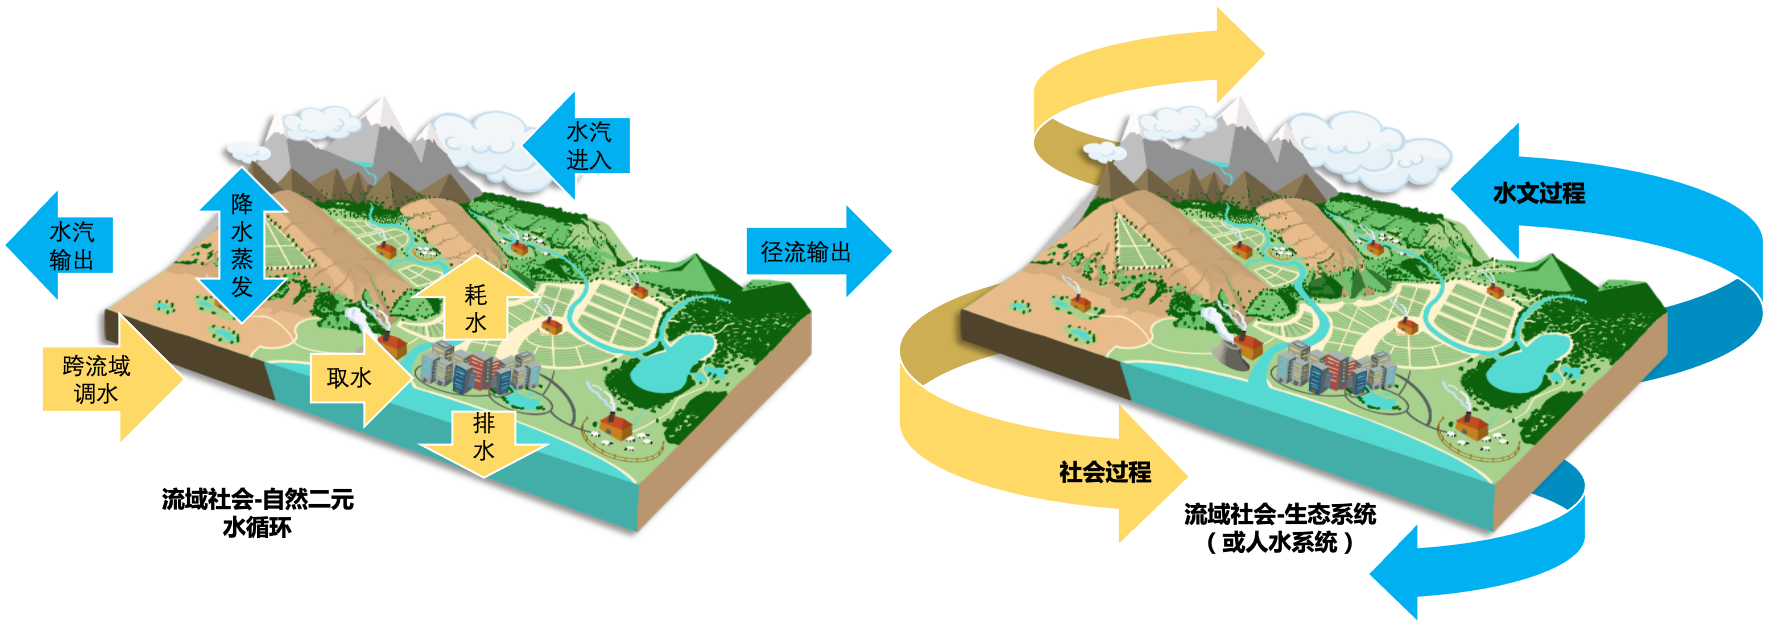
\includegraphics[width=\textwidth]{img/ch1/ch1_two_water_cycle.png}
    \caption[流域人水耦合系统的典型理论示意图]{流域人水系统耦合的典型理论示意图\cite{wang2006,dibaldassarre2015}。蓝色代表自然水循环的典型过程;黄色代表社会水循环的典型过程。}\label{ch1:fig:two_water_cycle}
\end{figure}

\subsubsection{社会-水文学}

% 开题报告
社会-水文学旨在理解人-水之间协同演化规律和循环互馈机制,多年来在现象检测、机理分析、模型预测等方面都获得了长足发展\cite{sivapalan2012, blair2016, srinivasan2016}。
社会-水文学在诞生之初便以流域系统为单元分析人与水的互动反馈过程(图~\ref{ch1:fig:two_water_cycle}右),其最根本的特征是将社会-水文系统视为动态系统,并将人类社会相关变量作为系统内部的驱动力,而非像传统水文学那样假设水文系统是在人类外部干扰下处于平衡态的\cite{sivapalan2012}。
Konar等人将社会-水文学的主要研究方向总结为四个:水循环与水资源利用、人与干旱之间的相互作用、人与洪水之间的相互作用、人与政策制度的相互作用\cite{konar2019}。
Yu等人则指出该学科经多年发展后呈现出三个特征:在水循环的不同时空尺度下开展研究、将人类文化的演化特征纳入研究、将基础设施建设对水循环的干扰纳入分析\cite{yu2020}。
在这种超越传统水文学的思想指导下,一些社会-水文现象得到揭示,例如增大用水效率却常常无法节约流域水资源的“用水效率悖论”\cite{grafton2018, xiong2021a},以及流域管理策略常在开发和保护之间周期性摆动的“钟摆效应”\cite{kandasamy2014, roobavannan2017, mostert2018}。

社会-水文学的发展同时也面临着诸多挑战。
Troy 等人通过文献分析,认为社会水文学研究尚集中在数据收集与整理、数据观察与推测、理论模型建立三个阶段,还缺乏对成熟的参数率定与模型预测,因此其预测能力相对较差,对指导政策制定还相去甚远\cite{troy2015}。
Sanderson 认为这种糟糕的模型表现很大程度上因为社会水文学并没有真正将社会因素纳入考量,因而发出了“社会-水文学需要社会科学”的呼吁\cite{sanderson2017}。
然而,社会科学常常没有统一、公认的理论,且人的主观能动性与文化变量均难以被模型捕捉。复杂系统的科学思想能够将复杂的人类行为纳入分析框架,被认为是社会-水文学未来重要的前进方向之一\cite{ahlstrom2021}。
综上所述,社会水文学的发展让人们对水问题背后的机制有了更深入的了解。分析与水相连接的社会动态是对传统的水文学的补充。但仍需要进一步在方法学上突破,结合多学科背景和复杂系统思想来分析社会-水文系统,以突破上述瓶颈。


\subsubsection{流域社会-生态系统}

% Handbook 什么是社会-生态系统
社会-生态系统的概念最早诞生于20世纪90年代中期,是生态经济学和公共池塘资源系统学者之间的跨领域研究,通过结合系统科学方法和适应性管理提出\cite{biggs2021},此概念有助于整合水的自然/社会属性研究\cite{fowler2022}。
它是一个典型的复杂适应性系统(complex adaptive system),由许多互相独立的部分组成,并以涌现的方式相互作用,系统层面的格局难以由某部分的属性来预测\cite{schluter2019}。
因此,社会-生态系统不等同于社会系统与生态系统的简单加和,而是由社会和生态组分之内/之间反馈所塑造的有机整体\cite{biggs2021}。
社会-生态系统理论发展至今已经产生了许多流行的框架,包括 Folke 和 Berkes提出的社会-生态系统概念框架\cite{berkes2008};将系统弹性描述为不同尺度适应性循环结果的扰沌框架\cite{gunderson2001};Liu 等人提出的远程耦合框架\cite{liu2018};Ostrom 分析公共池塘资源的社会-生态系统诊断框架\cite{ostrom2009};Schluter 等人提出的社会-生态系统行动情景框架等\cite{schluter2019}。

随着可持续发展目标的提出,社会-生态系统理论在21世纪得到广泛认可,作为跨学科概念反哺社会-水文学,逐渐形成了“流域社会生态系统”的概念。
Huggins对全球流域社会-生态系统在水资源压力下的脆弱性进行了评估,分析了淡水资源压力不断加剧对社会-生态系统的潜在影响,识别了全球的热点流域\cite{huggins2022}。
Varis综合考虑了社会系统的三种适应力和生态系统的三种脆弱性因素,在全球尺度评估流域社会-生态系统在弹性和适应之间的平衡\cite{varis2019}。
国内也逐渐接受流域系统是社会-生态系统或复杂系统的观点,重视系统科学在流域综合研究中的重要性。
程国栋和李新在“黑河流域生态-水文过程集成研究”中提出了流域科学的概念,将流域视为地球系统的缩微,考虑水文和生态系统的自组织性如何影响流域系统的功能,以及人的因素如何被集成到流域水文学和流域生态学中\cite{cheng2015}。
傅伯杰等人指出亟需聚焦人地系统耦合机理与调控途径,揭示黄河流域人水关系演变及社会-水文-生态系统动态\cite{fu2021a}。
一些实证研究也开始从不同角度分析流域社会-生态系统,包括结构变化\cite{song2022}、制度变化\cite{wang2019d}、社会意识\cite{liu2023}等对系统局部、流域系统、外部系统等产生的不同影响,证明了思想与社会-生态系统理论对流域研究的重要性。

\subsubsection{人水关系与人水系统}

正如中文语境的“人地关系”在英语世界一般等价于“human-environment interactions”\cite{li2016c, liu2023},“人水关系”直译的“human-water relationship”也并非英文世界的常见关键词,取而代之的是通常不限定时空尺度的术语“human-water systems”,即人水系统\cite{konar2019}。
人水系统是以水循环为纽带,将人文系统和自然系统联系起来并组成的复杂系统,能依靠自身循环动力和经济发展动力而演变\cite{zuo2007},也是一类典型的社会-生态系统,因此“流域社会-生态系统”与“流域人水系统”通常同义\cite{yu2020}。
左其亭认为中文语境常用的概念“人水和谐”不曾有严谨的学术定义\cite{zuo2007},指出“人水关系”应指人水系统中“人文系统”与“水系统”之间的关系,“人水和谐”则是对人水系统要素间关系的评价,并在此基础上提出了与“人水关系和谐论”与“人水关系学”\cite{zuoqiting2022, zuo2016a}。
但是,“人水关系学”侧重对人水系统进行整体评价,以指导水资源分配与流域管理,因此“人水关系”仍需被具体化为人类与水资源的多种互动关系\cite{zuo2016, zuo2020a}。

综上所述,许多理论框架,如“自然-社会二元水循环”、“社会-水文学”、“流域社会-生态系统”和“人水关系学”,从不同侧重点出发重视水的自然-社会双重属性研究。
其中,“自然-社会二元水循环”基于平衡态假设,已对多个流域在人类影响下的水平衡模式进行了计算与建模,服务于水资源管理工程;“社会-水文学”关注“人”与“水”之间的协同演化,在非平衡态假设下揭示了流域演变规律;“流域社会-生态系统”或“流域人-水系统”的概念结合了社会水文学与系统科学,强调整体性和协同演化的复杂性,是目前流域系统研究的前沿。
然而,目前流域尺度上仍缺乏对“人水关系”的具体定义,相关研究在不同时空尺度下均使用过于宽泛的“人水关系”概念,这给分析流域人水系统的演变过程与演变机制带来了阻碍。
鉴于在实际研究中,研究者绝无可能穷尽流域人-水系统的全部作用关系,本研究将“人水关系”的涵义界定为:人类活动直接改变水圈要素、过程,或人类决策反之受到水圈要素、过程不可被忽略的干预或影响时,人与地球表层系统的相互作用。


\subsection{人-水关系的演变过程}\label{ch1:sec:process}
协同演化路径的多样性体现了人水系统的复杂性,其演变过程也是流域社会-水文研究的热点。从侧重点不同可将目前研究分为“概念模式变化”、“关键指标变化”和“结构功能变化”三个方面。

概念模式是对许多共性规律的高度抽象或理论总结,以便研究人员和决策者在宏观层面把握人水系统的演变过程;关键指标则通过能够表征流域系统的关键变量或综合指标的变化规律来把握流域演变过程;而结构功能变化则是通过流域系统内重要组分的相互关系变化,以及与这种变化相关的系统功能改变来把握流域演变过程。

\subsubsection*{人水系统的概念模式变化}

在人水系统演变研究中,可以借鉴其他学科或领域的已有理论或概念,总结其概念模式的演变。
例如张家诚(2006)从科学哲史和科学哲学的角度出发回顾人水关系的演变历史,指出人水关系从古代时“天-地-人的平衡中庸模式”,到近代工业社会变为在追求自己的发展时忽略自然环境的“数学模式”,同时展望了信息时代人水关系的“工程调控模式”\cite{zhang2006}。
于宏瑞认为人-水关系是随着社会发展而变化的,因此经历了自然崇拜、趋势利用、盲目开发、持续协调四个阶段\cite{yuruihong2011}。
Gleick 和 Palaniappan 借鉴“石油峰值”为流域提出了“水峰值”的概念,借助该概念可将流域潜在水供应分为三个变化阶段:阶段一随着用水需求的增加可用水资源的供应(新修水坝、水库、泵);一旦达到最大成本效益的地表水和地下水开采;有一个最终转移到一个更高的成本支撑的供应水如海水淡化或转移等各种来源的增量增加供应\cite{gleick2010}。

人水系统演变的概念模式还可以通过流域的实际发展规律总结得出,这类模式通常有更活跃的理论生命力,也更能有助于指导后续研究和决策。
1999年,Turton提出了影响深远的“流域适应能力”概念框架,该框架指出,根据水资源的供需关系,流域人水系统随着发展可能依次在“获取更多水资源供应”、“提高用水效率”、“提高分配效率”、“适应水短缺状态”四种原型模式间演变\cite{turton1999}。
该框架在澳大利亚流域水治理改革案例中的应用不仅佐证了其重要指导意义,还暗示了流域演变过程可能还存在水需求下降的“第五阶段”\cite{loch2020}。
另一个典型的案例是通过澳大利亚东部 Murrumbidgee 河流域总结出的“钟摆效应”模式,它说明了流域人水关系在取水用于粮食生产和努力缓解流域环境退化之间保持动态演进,并在摇摆间将流域人水系统演变划分为四个时期\cite{kandasamy2014, roobavannan2017},而这一规律随后也在中国和欧洲等更多区域得到了复现\cite{han2017, mostert2018}。

\subsubsection*{人水系统的关键指标变化}

由于人水系统的复杂性,研究常从不同角度切入构建综合指标,用以表征人水关系的变迁。
刘海猛等人基于复杂自组织系统理论,在辨析人水系统基本内涵的基础上提出了人水关系演化的概念模型,将人水系统的演变过程概念化为社会经济、生态环境、水资源开发利用三个变量组的函数关系\cite{liu2014}。
Zuo 等人将“和谐人水关系”指标分为健康度、发展度、协调度\cite{zuo2008},该综合指标可将中国的人-水关系分为二十世纪中期以前、1950年至1980年、1980年至1990年、1990年之后四个时间阶段,各阶段的流域人水关系的主要特征分别是:应对用水需求和水灾、管理供水和去中心化、依法管理水资源、高度重视人水和谐\cite{zuo2016a}。

这种通过关键指标识别人水关系的方法须广泛收集来自不同领域的数据,在时间序列数据收集和数据同化上存在诸多挑战,但其优势在于一旦数据可用,能同时对全球各大流域进行大规模计算与分析。
Varis等人基于三个社会系统的适应性指标和三种生态系统的脆弱性指标,构建了综合指数评估流域社会-生态系统在弹性和适应之间的平衡,分析了各流域通过发展提升适应性的演变过程\cite{varis2019}。
Huggins等人则更侧重流域在水资源压力下的脆弱性,通过全球各流域的水资源可用性指标和人类面对压力的适应指标,综合分析了不断加剧的淡水资源压力对流域社会-生态系统的潜在影响路径\cite{huggins2022}。
Qin等人提出的稀缺性-韧性-易变性(SFV)指标,考虑了管理措施(如水库的建设)和用水结构变化(有些用水方式如能源用水是难以被短期替代的),选择了三个子指标对流域人类活动情况下水资源短缺情况做出评估,并分析了不同发展程度的地区在面对水资源短缺时的可能发展路径\cite{qin2019}。

\subsubsection*{人水系统的结构功能变化}

流域系统的结构变化是实现功能改变的必要条件,二者通常伴随着变化,因此寻找决定系统功能的关键变量,最直接的方式是通过结构变化识别流域人水关系演变。
例如,Wang等人提出了“矛盾统一”的人水关系理论框架,通过识别人与水之间是否是“对抗”关系,在两千年时间尺度上拟合了中国的人水关系变化\cite{wang2017}。
另一组常用于表征流域人水关系演变的要素是水、粮食和能源,但 Rollason 的研究指出,这三者之间的关系可能比许多研究中所表达的更为复杂\cite{rollason2021}。
因此,在利用关键要素间的关系进行识别时,需要精确把握关键变量,包括哪些要素需要纳入分析,以及如何构建它们之间的关系\cite{zhangzongyong2020, wang2021}。

改进上述问题的一个思路是使用复杂网络分析方法,尽可能考虑当前人水系统中所有需要考虑的因素,然后使用复杂网络指标分析系统演变\cite{sayles2019, bodin2017b}。
例如,Song 等人基于经济复杂性概念,使用全国的年均虚拟水足迹数据集(1978年至2008年)构建了农产品-虚拟水转移量的二分网络,通过复杂网络分析计算了网络复杂性随时间的变化,进而分析黄河流域水资源的重要性演变规律\cite{song2022}。
Sayles 等人结合生态和生态修复政策的数据,构建了流域的社会-生态网络,发现存在潜在结构问题的区域合作网络的密度和生产力都最弱的\cite{sayles2017}。
要识别网络结构,需要收集相对全面的关系数据集,并且对数据质量要求较高,这在一定程度上限制了此种研究方法的广泛应用。

最后,还可以直接从系统功能的角度出发寻找表征系统演变的证据,该方法易于在不同流域系统中使用,但依赖对人水系统功能的正确认识,因此得到广泛认可的方法指标相对较少。
Falkenmark 等人提出的“蓝水”和“绿水”概念\cite{falkenmark2006},以及后来提出的“灰水”,都是典型的从系统功能角度出发,研究流域结构-功能变化的理论框架\cite{mekonnen2011}。
传统水资源规划和管理针对的重点仅是河道的液态水(蓝水),大多数在流域面上以降水和蒸散的形式参与循环(绿水),此外还有少部分经人类利用后又参与循环的水资源(灰水),三者在流域人水系统中承担着截然不同的功能\cite{craswell2007}
随着流域社会经济发展和气候变化,流域水循环各部分的绿水和蓝水比例都会发生变化,这将对人水系统功能产生极为深远的影响,如降低弹性、削弱流域系统的生态系统服务、甚至导致系统崩溃\cite{falkenmark2019}。

综上所述,当前人水系统演变过程可以通过“概念模式变化”、“关键指标变化”、“结构功能变化”三个方面进行分析和总结,但仍需要加强三类框架之间的互相联系。如果流域人水系统的变化足够显著,上述三方面的研究理应是殊途同归的:通过识别关键指标变化的阈值,结构-功能表征系统整体变化,并对变化前后的系统状态做概念化总结。


\subsection{人-水关系的稳态转换}\label{ch1:sec:mechanism}
% 流域人水系统是典型的社会\textendash{}生态系统,系统演变机制是社会\textendash{}生态系统研究的核心内容。
% 根据侧重点的不同,武旭同将当前社会\textendash{}生态系统互馈的机制总结为“时”(系统弹性)、“空”(全程耦合)、“构”(结构匹配)、“阈”(地球界限)四个方面,其中“时”为包含弹性和稳态转换在内的一组概念,是研究社会\textendash{}生态系统动态演化的重要理论框架,对理解人水系统的演变机制至关重要\cite{WuXuTong2021}。
% 本节综述了与稳态转换密切相关的核心概念,并分别围绕“驱动因素、表现特征、级联效应”三个稳态转换的核心要素,总结了分析人水系统演变机制的主要路径。

\subsubsection{稳态转换与相关概念}

% 宋嘉熙 的 地理学报
弹性(Resilience)是指处于动态平稳的系统面对变化时通过缓冲、适应或转变等方式响应得以维持的能力\cite{folke2010}, 稳态转换(Regime shifts)指系统的结构和功能发生大规模重组并突破这种平稳状态的过程\cite{scheffer2001},在生态系统、气候系统、经济系统、及其它复杂系统中均可能发生,具有不易预测、难恢复的特点\cite{scheffer2003, biggs2009}。
通常使用“球-杯模型”或“折叠二分模型”来描述稳态转换。
以“球-杯模型”为例,不同稳态就像系统状态空间中凹陷的“杯子”,将系统实际状态则如同在不同凹陷间滚动的“小球”,状态空间的变化(参量驱动)或小球受到外力(变量驱动)时都可能推动系统状态在不同稳态间发生转换\cite{scheffer2009, folke2010}(图\ref{ch1:fig:regime_shift})。
稳态转换的诱发机制可以从参量驱动和变量驱动两个方面入手,前者是指外界条件(环境参数)发生变化时削弱系统弹性导致的稳态转换,后者是指系统内部或外部变量推动系统突破阈值从而触发的稳态转换\cite{scheffer2009, folke2010}(图\ref{ch1:fig:regime_shift})。
除了驱动因素外,系统稳态转换的发生可能致使系统功能与产出(Outcome)发生变化,或进一步触发其它的级联效应(Cascading Effect)\cite{rocha2018}。
因此,识别稳态转换应从“驱动力-现象-效应”这三个稳态转换的核心要素切入,从而厘清系统间反馈机理、分析关键要素间交互作用,揭示社会\textendash{}生态系统稳态转换的成因类型、现象特征与产出/外溢效应。

% Description of system regime shift by ball-cup model and fold bifurcation
\begin{figure}[!ht] % use float package if you want it here
    \centering
    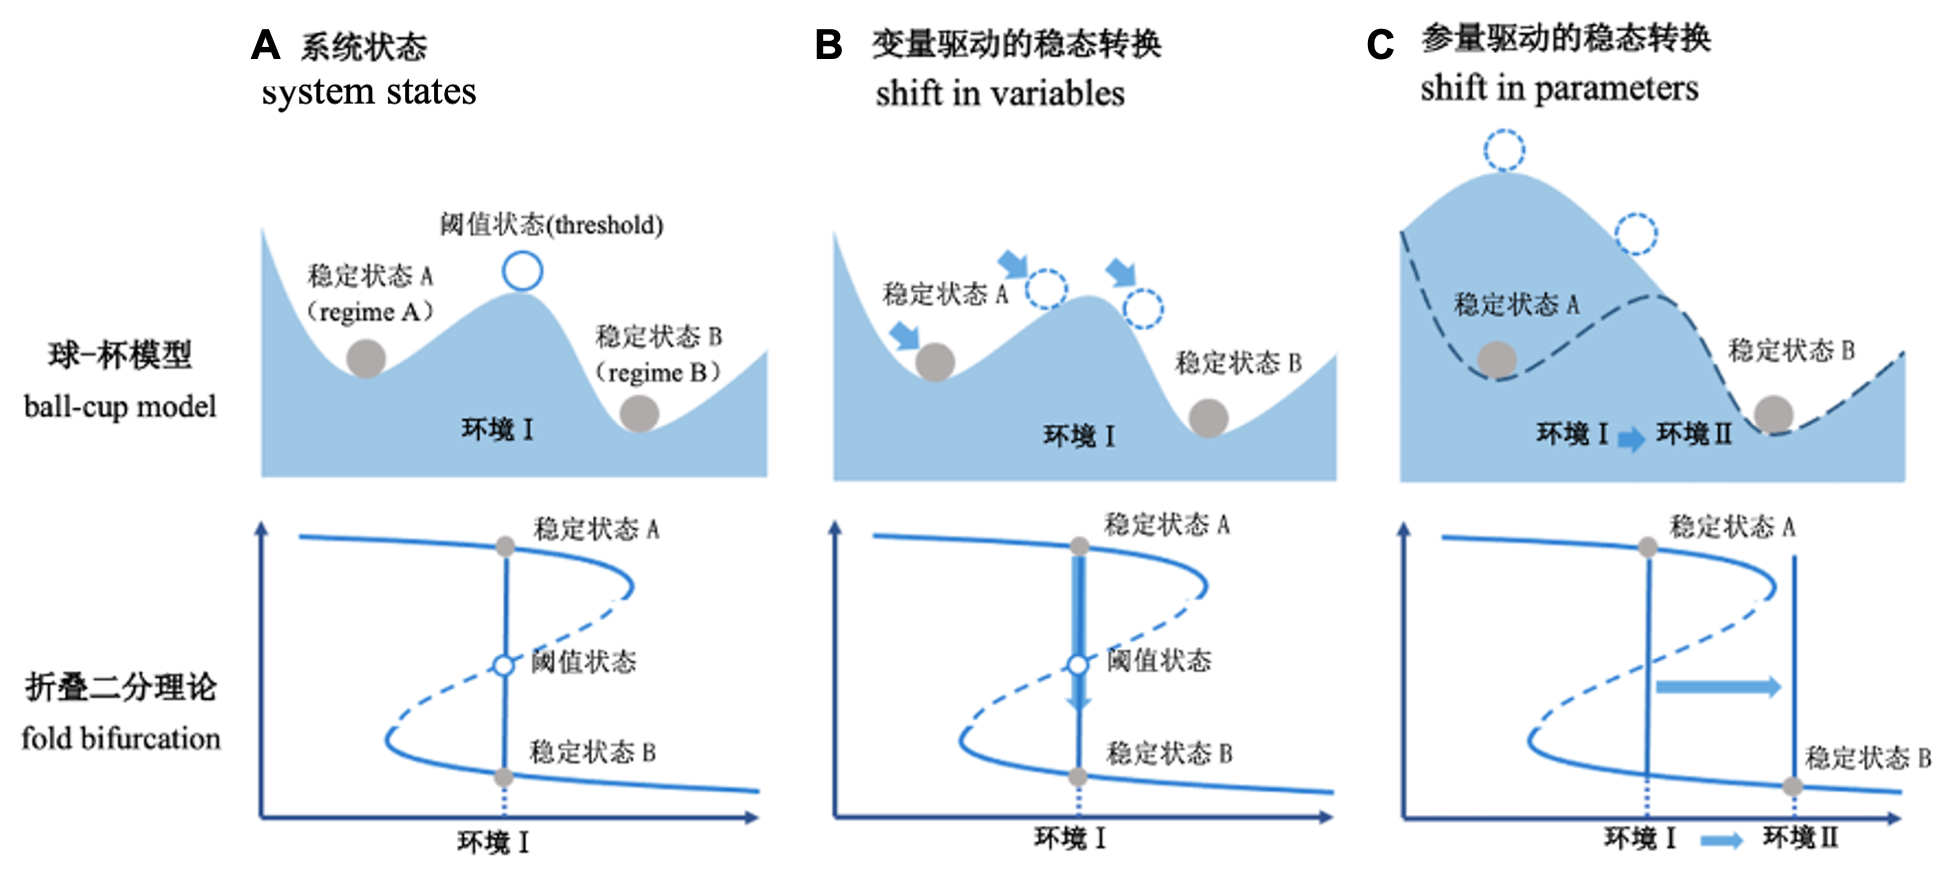
\includegraphics[width=\textwidth]{img/ch1/ch1_regime_shift.png}
    \caption[系统的稳态转换理论框架]{系统的稳态转换理论框架。
    \textbf{A}假设系统中存在稳定状态A和稳定状态B,球-杯模型(ball-cup model)和折叠二分理论(fold bifurcation)对系统各种状态的表征。
    \textbf{B}系统稳态转换过程。变量驱动的稳态转换(shift in variables):环境\romannumeral1不变时,处于稳定状态A的系统在干扰下自身突破阈值状态转换为稳定状态B。
    \textbf{C}参量驱动的稳态转换。环境\romannumeral1变为\romannumeral2,迫使处于稳定平衡状态A的系统向新环境下仅存的稳定平衡状态B转换。}\label{ch1:fig:regime_shift}
\end{figure}

\subsubsection{稳态转换的驱动因素}

Rocha等人发现,不断累积的人为干扰压力和气候变化是最常见的两类稳态转换驱动因素,无论以变量还是参量的形式出现\cite{rocha2018}。
Ji等根据水-沙调节方案和河口河道迁移这两个主要驱动因素变化的时间节点,结合不同阶段河口侵蚀-沉积量与河口排沙量,确定了河口侵蚀-积聚模式的稳态转换过程\cite{ji2018}。
Bao等在分析黄河中游水平衡系统稳态转换时,识别出气候驱动因素和土地利用/覆盖显著变化的阶段。通过验证不同阶段水平衡状态的差异确定了不同稳态阶段,并进一步定量解析了驱动水平衡状态转换的具体机制\cite{bao2019}。
此类分析路径的关键在于准确选择系统驱动力的定量表征,因此需要预设系统稳定状态和驱动力之间的关系。
这种方法多用于驱动力易于识别的干扰因素,如持续减少的林地、持续周期性变化的气候等。

“稳态循环”理论有助于理解另一类常见的人为干扰——流域治理措施——驱动的稳态转换。
该理论认为系统在不同尺度下都可以自组织历经适应性循环的“开发”、“保护”、“释放”、“更新”四个阶段\cite{gunderson2001},之后又进一步总结为“涌现”、“制度化”、“更新”三个阶段。
基于“主动改变不良的社会\textendash{}生态系统状态”与“调节并维持良好的社会\textendash{}生态系统状态”两种不同的目的,治理措施可分为自上而下的“转型治理”和自下而上的“协作治理”两类\cite{song2019}。
转型治理关注社会\textendash{}生态系统的释放和更新阶段,强调适应性治理的实现和主动促使社会\textendash{}生态系统完成状态的更新;协作治理则强调适应性治理制度化过程,旨在通过利益相关者间自组织的协作模式来实现社会\textendash{}生态系统的开发与保护\cite{song2019}。
因为无论自上而下或自下而上,流域治理既可能维持稳态,也可能触发稳态转换,需要在分析流域治理措施的作用机制时加以甄别。

\begin{figure}[!ht] % use float package if you want it here
    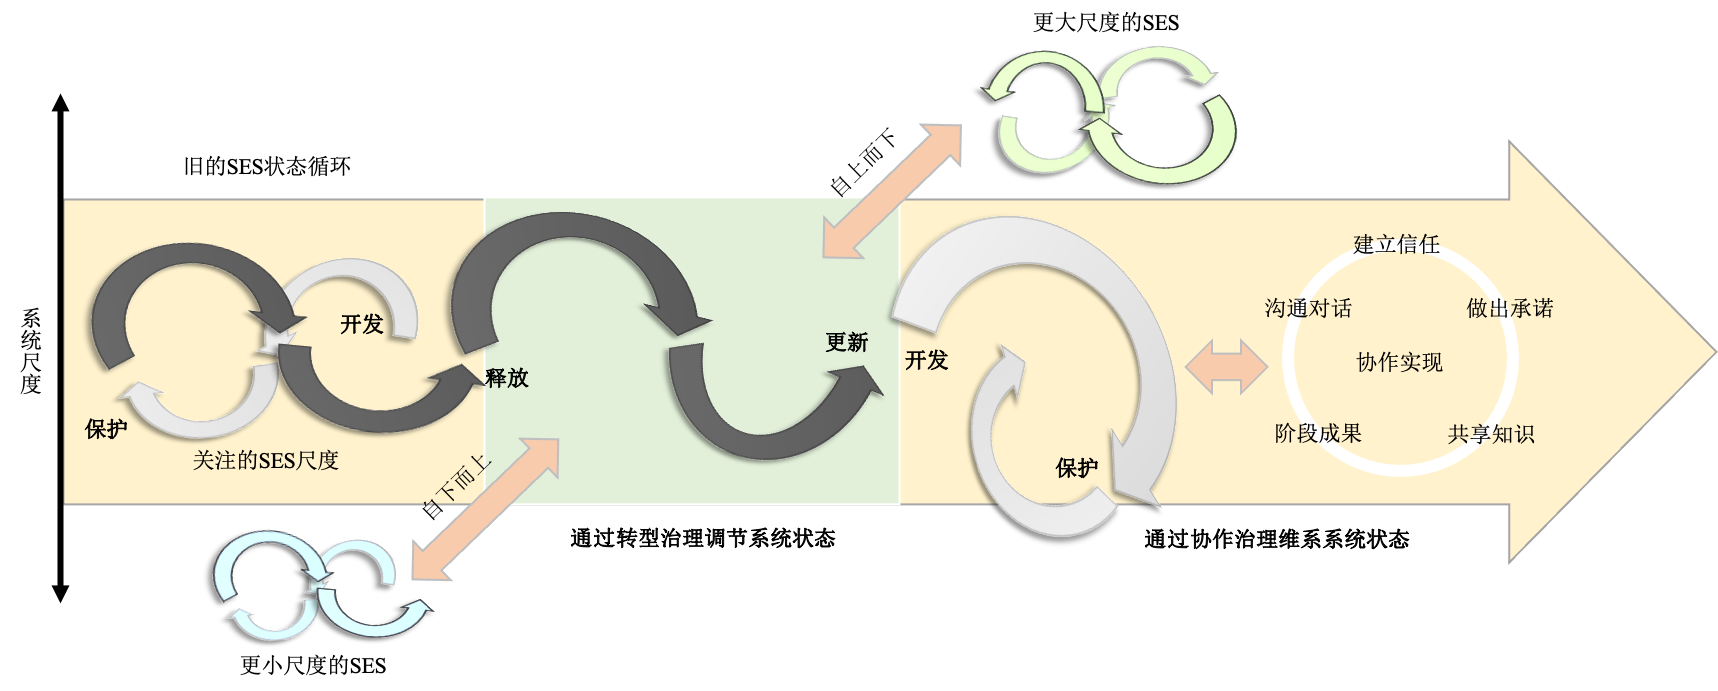
\includegraphics[width=\textwidth]{img/ch1/ch1_governance_driver.png}
    \caption[社会\textendash{}生态系统状态循环]{社会\textendash{}生态系统状态循环与转型治理、协作治理的关系。
    % Fig.4  The relationship between social-ecological system adaptive cycle and transition / collaborative governance
    图中展示旧的社会\textendash{}生态系统(SES)因转型治理而进入新的状态循环,并因协作治理的实现而延长开发保护阶段的过程}\label{ch1:fig:governance_driver}
\end{figure}

\subsubsection{稳态转换的表现特征}

聚焦于稳态转换过程中所表征出的现象是分析稳态转换最常见的路径,通过寻找合适的指标识别系统互馈变量或相关解释变量的趋势突变,检测稳态转换现象。
相关的检测方法非常丰富,常见的包括趋势分析、突变点检测或断点回归等。
Wang等利用t检验的循序算法和加性季节和趋势断点模型两种方法检测$1950 \textendash{} 2011$年黄河流域上中下游径流和输沙量的突变时间点以确定稳态转换时期\cite{wang2014};
Zhao等利用曼-肯德尔(Mann-Kenall)趋势分析法和加性季节和突变点检测模型识别出1921—2011年期间黄河月径流量趋势突变,重建天然径流量,量化人类活动对流量稳态转换的影响程度\cite{zhao2015}。

在识别稳态转换现象的基础上,还可以进一步将其与稳态转换驱动力相关联。
Yang等利用 Pettitt 检验计算稳态转换指数,探测流域径流的稳态转换,并与气候和土地利用变量的突变点对比分析,证实土地利用政策驱动了径流的稳态转换\cite{yang2012a}。
Niu等检测了黄河三角洲系统降水量,温度,月径流量和归一化植被指数(Normalized Difference Vegetation Index,NDVI)等多个现象相关变量共同的分解趋势断点,识别水文\textendash{}气候\textendash{}植被系统的稳态转换时期,分析各阶段内气候水文变量与NDVI间产出效应\cite{niu2020}。
虽然聚焦于稳态转换现象表征易于直观划分稳态转换的时期,且有着成熟的数据检测技术,但如果忽略对驱动和效应的结合分析,容易对稳态转换的驱动-响应机制表达不够全面。

\subsubsection{稳态转换的级联效应}

级联效应是指系统稳态转换后所产生的一系列后续影响,通过分析级联效应,可以更好地理解系统内部互馈关系的复杂性\cite{rocha2018}。
根据受到影响的要素在系统内或系统外,级联效应可分为内联效应和外溢效应\cite{rocha2018}。
在研究稳态转换时,Sun等利用沉积率曲线参数变化来刻画泥沙运输稳态转换的产出效应变化特征,同时解释了生态恢复对泥沙运输稳态的调节作用\cite{sun2020};
Wu等在研究黄土高原社会\textendash{}生态系统稳态转换时,通过量化社会\textendash{}生态系统内部要素交互作用的稳定状态,揭示了稳态转换不同阶段内系统关系变化和外溢效应\cite{wu2020a}。
Kidder等在研究黄河河道泥沙淤积系统稳态转换时,利用外溢系统中黄河下游洪水的频率和规模变化确定稳态转换发生时期,指出堤坝作为驱动因素对泥沙淤积存在着强烈正反馈\cite{kidder2015}。
此类分析路径有助于识别复杂的社会\textendash{}生态系统稳态转换的发生机制,正成为稳态转换实证研究的热点,但需要准确选择与系统反馈过程联系紧密的级联现象,因此也需要关于系统稳态的先验知识。

总的来说,虽然已有很多研究从驱动因素、表现特征和级联效应等不同方面探究人水系统的稳态转换机制,并提出了相应的量化方法,但稳态转换是大规模的系统重组,需要考虑多个要素的同步变化。
仅从单一要素出发的研究容易导致对其机制认识不全面,因此需要进行系统整合,探讨“驱动-现象-效应”的多要素联合变化。


\subsection{人-水关系建模}\label{ch1:sec:model}


% 开题报告
模型的建立是为了理解、描述和预测自然界,应当在真实性、预测性、普遍性之间达到均衡[27],流域系统模型通常旨在表征水的地球物理过程的动力学,以及人类用于管理系统的元素,如基础设施、机构和治理。 %\cite{hadjimichael2020}。
流域人水系统既有空间尺度依赖的地表生态过程,也有系统层次变量反馈的动力过程,还有多尺度的复杂人水相互作用[47–49]。
相应地,流域人水系统的建模主要有基于传统分布式水文模型耦合人类活动模块发展而来的分布式社会-水文模型、在系统或区域层次上耦合来自社会、自上而下模拟生态系统关键变量的系统动力学模型、自下而上对流域内复杂人-水互动进行仿真的多主体模型。

\subsubsection*{分布式社会-水文模型}

% 焦 本研一体 本子
与传统的集总式水文模型相比,分布式流域水文模型不再将流域视作均匀的整体,充分地考虑了流域内水文过程的异质性[207],是流域研究的主流工具,常见的分布式水文模型如如SWAT模型、新安江模型、陕北模型、布式时变增益水循环模型等(徐宗学,2019)[208-210],在国内外都得到了大量应用[211-213]。 % 焦 本子
% [207]王中根,刘昌明,吴险峰.基于DEM的分布式水文模型研究综述[J].自然资源学报,2003(02):168-173.
% [208]J. G. Arnold,R. Srinivasan,R. S. Muttiah,J. R. Williams. LARGE AREA HYDROLOGIC MODELING AND ASSESSMENT PART I: MODEL DEVELOPMENT[J]. JAWRA Journal of the American Water Resources Association,1998,34(1):73-89.
% [209]王中根,刘昌明,黄友波.SWAT模型的原理、结构及应用研究[J].地理科学进展,2003(01):79-86.
% [210]夏军,王纲胜,吕爱锋,谈戈.分布式时变增益流域水循环模拟[J].地理学报,2003(05):789-796.
% [211]Karim C. Abbaspour,Jing Yang,Ivan Maximov,Rosi Siber,Konrad Bogner,Johanna Mieleitner,Juerg Zobrist,Raghavan Srinivasan. Modelling hydrology and water quality in the pre-alpine/alpine Thur watershed using SWAT[J]. Journal of Hydrology,2006,333(2):413-430.
% [212]Darren L. Ficklin,Yuzhou Luo,Eike Luedeling,Minghua Zhang. Climate change sensitivity assessment of a highly agricultural watershed using SWAT[J]. Journal of Hydrology,2009,374(1):16-29.
% [213]Gangsheng Wang,Jun Xia,Ji Chen. Quantification of effects of climate variations and human activities on runoff by a monthly water balance model: A case study of the Chaobai River basin in northern China[J]. Water Resources Research,2009,45(7).
% 江 本子
流域分布式模型通过耦合生态过程,可用于描述大尺度流域陆地生态演变过程的生态水文模型,如SWIM模型(Krysanova等,2005)、RHESSys模型(Tague和Band,2004)、Budyko–Choudhury–Porporato模型(Donohue等,2012)、EHSM模型(Viola等,2014)、HYMOD-BGM模型(Tang等,2018)等。
国内的包括EcoHAT模型(刘昌明等,2009)、WEP-IBIS模型(Cao等,2015)、CLM-GBHM模型(Jiao等,2017)、GBEHM模型(Qin等,2017)、BEPS-TerrainLab模型(Chen等,2007)、HEIFLOW(Tian等,2018)等。

% 焦 本子
现有的分布式水文模型由于构建原理及最初率定区域不同,导致模型侧重点有所不同。如SWAT模型侧重描述产流过程[209],LISTFLOOD模型侧重模拟水动力过程、洪水过程等[217],但现有的分布式模型仍较少将人为干预水文过程的因素作为模拟重点,
% [209]王中根,刘昌明,黄友波.SWAT模型的原理、结构及应用研究[J].地理科学进展,2003(01):79-86.
% [217]曾照洋,王兆礼,吴旭树,赖成光,陈晓宏.基于SWMM和LISFLOOD模型的暴雨内涝模拟研究[J]
贾仰文等人WEP-L分布式流域二元水循环模型(简称 WEP-L 模型)是具有物理机制的流域分布式水循环模型,考虑了人类取用水和水利水保工程等因素对水循环过程的影响,实现“自然-社会二元水循环”过程耦合模拟和分析。 % todo citation
2019年,国际应用系统分析研究所(International Institute for Applied Systems Analysis, IIASA)开发了基于社区的水文模型模型(Community Water Model, CWatM)模型,将水库调度等水资源管理要素也纳入了模型[218]。
但迄今为止,仍鲜有将水资源治理制度(如法律法规)等人类活动要素的影响作为流域分布式模型模拟的重点。
% [218]Peter Burek, Yusuke Satoh, Taher Kahil,et al. Development of the Community Water Model (CWatM v1.04)- a high-resolution hydrological model for global and regional assessment of integrated water resources management[J].GEOSCIENTIFIC MODEL DEVELOPMENT,2020,13(7):3267-3298.

\subsubsection*{自上而下的系统动力学模型}

% 江本子
系统动力学模型能够自上而下地解析系统层面的要素关联、反馈与演化(Jaeger等,2017;Jiang等,2022),可预测变化环境下关键变量及其反馈过程的变化(Vaighan等,2017)。
许多大尺度的评估模型都是系统动力学模型,有 ANEMI3、 ANEMI Yangtze,以及在中国区域建立的 T21 China 模型,三者均包含自然和社会系统的多个部门,反映自然和社会系统的相互作用。
因此,流域人水系统的系统动力学模型可以通过分析系统间的相互作用、内部结构变化等现象,揭示流域人水关系的动态特征,如 ANEMI Yangtze 是在 ANEMI3 的基础上在长江流域建立的系统动力学模型。
将空间范围限制在流域尺度的系统动力学模型可以在建模过程中考虑研究区特征,使模拟结果更符合流域系统的实际情况,例如 ANEMI Yangtze 将长江的渔业作为模型的外生变量纳入考虑,分析了十年禁渔政策对流域系统的影响。 % todo citation

人类活动还可以作为系统内部反馈循环的关键变量被纳入模型。
% 开题报告
Viglione 和 Baldassarre 等人在流域尺度构建了用于解释和预测人类社会与洪水互相反馈、协同演化的系统动力学模型,其中水文要素(洪水)和社会组分(如公众意识、风险文化、经济发展等)都是反馈过程的核心变量[43]。
Muneepeerakul 等人(2017)则提出了一个流域社会-生态系统的发展轨迹模型,以探讨在什么情况下稳定的治理结构可以在促使堤坝等公共基础设施在系统中内生地出现\cite{muneepeerakul2017}。
系统动力学的劣势也很明显,首先是缺乏对空间特征的识别,这对流域系统是至关重要的;其次是通常需要自上而下对系统要素间关系给出基于数据或经验的函数假设,对于较为复杂且尚缺乏充分研究的流域系统变化,建模即便不是不可能,也将是非常困难的。

\subsubsection*{自下而上的多主体模型}
% 开题报告
涌现(Emergence)指系统实体会产生其所有组成部分本身没有的属性,人-水系统作为开放的复杂巨系统,广泛存在的相互作用就是宏观演化属性涌现的关键[51]。
% 来自 chat GPT
流域人水系统的多主体模型是指在研究人类活动对水资源的影响时,将不同的相关主体,如政府、水用户、环境保护者等作为系统的不同主体分别进行考虑,并综合考虑它们之间的相互影响关系,以达到更加全面、系统地研究人水关系的目的。这种模型在人水关系研究领域越来越受到关注,为了更好地研究人类活动对水环境的影响,并为流域水资源管理提供有力的指导。

自组织(Self-organization)是指一种起源于初始无序系统的部分元素之间的局部相互作用、所产生出某种形式的整体秩序的过程。这与复杂系统建模中自下而上的基于主体的建模(Agent-based model) 思想类似。
因此Castilla-Rho等人[61–63]利用多主体建模的复杂系统模拟方法将Ostrom发现的机制应用于地下水流域的管理模型中,发现可以解释地下水资源治理模式的涌现。但对于大河流域来说,由于人能直接观察到流动的水资源变化,且存在明显的时空分异性,尚缺乏较好的复杂系统建模以探索其中人-水关系的核心演化机制。

自下而上模拟流域水资源使用时上中下游不同行业利益相关者的冲突、合作,及其相互作用下治理体系的整理结构与功能,逐渐成为流域可持续治理的重要基础[53,54]。


刻画人水关系的模型和计量手段日益丰富,如应用多主体模型揭示了逐水而居的本能可能是人类早期迁徙演化的重要驱动力[42];

由于人类社会系统和流域水文系统的结构和功能具有不同的尺度和动态,匹配是指两者之间的良好关系。
Sayles 2017 研究了流域尺度社会-生态的匹配

总的来说,基于复杂系统的建模已成为研究人-水系统的重要技术手段,能够基于水的资源属性对利益相关者的人-水互动进行理论机制上的探索。这种自下而上的建模思路与SES的自组织管理机制一脉相承,但目前比较成熟的模型主要关注地下水流域和,对河流的水资源治理,尤其是水资源稀缺的大河尚缺乏泛用性较强的机制模型。


\subsection{黄河的人-水关系研究}\label{ch1:sec:yellow_river}

% 开题报告
黄河是全球人与水关系变化最频繁、最剧烈、影响最深远的大河之一。
人类社会与黄河相互作用的研究历史悠久,例如魏特夫对黄河流域的社会发展历史进行了考察,提出了著名的“水利社会理论”,认为这样的大规模的治水活动是中央封建王朝皇权诞生的重要因素\cite{weitefu1989}。
但许多中国学者认为,魏氏的观点是颠倒了复杂人-水关系中的因果关系,正是中央皇权的强劲发展使得大规模治水活动成为可能\cite{jizhaoding1981}。
治水策略的选择是决定黄河河道演变的重要人为因素,同时河道的自然条件也是选择治理策略的重要依据,由两者共同决定的治理结果会形成路径依赖\cite{WangWeiJing2009}。
因此,为了总结黄河流域人与水关系的变化,不乏有着眼于总结演变过程的著作。
于瑞宏详细地梳理了黄河流域人-水关系演变的典型事件,并将其分为上游、中游和下游区域,但未能将其串联在一起\cite{yuruihong2011}。
同样,有一些研究倾向于按照黄河流域人-水关系的关键主题来梳理演变进程,并努力展示其时间深度和因果关系,例如,葛剑雄从黄河与中华文明互动的角度进行了梳理\cite{gejianxiong2020},王渭泾则从黄河治理的角度进行了梳理\cite{WangWeiJing2009},以总结近两千年来黄河人-水关系的演变历史。
然而,这些研究通常仅限于对人水系统进行“专题梳理”,并以描述性概念模型为主,无法对流域人水系统的演变进行定量分析,因此难以满足对未来演变方向作出科学解释的需求。

% 于璐 本子
黄河流域是人-水关系和社会-水文学研究的重要案例。
长期以来,该流域受到人类活动的强烈影响,其人水关系演变具有复杂性,因此是稳态转换研究的代表区域\cite{zuo2022, wang2014}。
目前的研究主要集中在评估人类活动对流域的影响、评估人为干预治理或资源管理的效果与影响等方面\cite{wang2016a, WuXuTong2021, wang2019c}。
在分析人-水系统关系演变机制方面,一些研究集中在指标和结构层面,如耦合协调度\cite{libo2022}、承载力\cite{wang2022d}、多维指标评价\cite{li2020}、网络\cite{song2022}和蓝水与绿水等\cite{zhuo2016a}。
但这些方法依赖于对长期、结构化时间序列数据的收集,因此很难应用于分析非工程性质的、非连续的流域治理制度等人水系统驱动力的机制。
总的来说,黄河流域人-水关系演变机制的研究对于非工程的水资源治理措施的影响机制探讨不足,因此很难对流域规划中政策影响下的未来情景进行预测。

针对黄河流域人与水文系统的复杂关系,也有一些研究采用了同时考虑人类活动和水文过程的模型。
例如,贾仰文等人基于WEP模型开发了WEP-L模型,通过划分子流域和等高带的方法实现了黄河历史径流的复现\cite{jiayangwen2005}。
杨大文等人构建了分布式水文模型,以表示黄河流域的多个水文参数\cite{yangdawen2004}。
岳瑜素等人应用了系统动力学模型,优化了黄河下游滩区自然、经济和社会协同的可持续发展模式\cite{yueyusu2020}。
Jiang等人建立了系统动力学模型,从社会、经济、资源、生态和文化五个方面预测了在未来政策情景下黄河流域的高质量发展水平\cite{jiang2021b}。
黄昌硕等人建立了基于“经济社会-水资源-生态环境”系统动力学模型,为动态预测区域水资源承载力的变化趋势和制定优化调控方案提供了参考依据\cite{huangchangshuo2021}。
% 自己写的
相比于广泛发展和应用的分布式水文模型和系统动力学模型,仿真黄河复杂人水系统相互作用和揭示涌现现象的多主体模型研究相对较少。
Cai 在水资源调度方面使用了多主体模型,以优化黄河流域的水资源分配。然而,他模拟的主体数量较少,且主体间的互动仅考虑了工程要素,与水资源管理的联合多目标优化相似\cite{cai2011}。
Du 等人在黑河这个黄河的子流域实现了分布式水文模型和多主体模型的耦合,分析了水政策、农民用水和水文条件之间的关系,并指出了区域水文地质条件(如地下水位深度和与河流的距离)是影响人类与水文相互作用的关键因素\cite{du2020}。
但是,在黄河流域研究中,仍缺乏考虑多级利益相关者的、从下而上的、耦合分布式水文模型的多主体模型,限制了对不同政策情境下黄河人水关系演变机制的分析与预测。

总的来说,现有的研究主要集中于梳理黄河人水系统演变的概念模型,缺乏从流域人水系统视角出发的定量分析;尽管对演变机制进行了定量分析和建模仿真,但多集中在水库等工程因素的影响上,忽视了流域水治理政策对人水关系变化的重要驱动作用。


\section{研究目标与内容及关键科学问题}\label{sec:contents}

\subsection{研究目标}
% 武旭同话术,待修改
基于上述研究进展,本研究面向社会-水文学研究前沿,以黄河流域为研究区,结合水文气象观测、社会经济统计、历史数据重建、遥感反演等获取多源数据,借助统计分析和模型模拟等手段,分析黄河流域人-水关系的演变过程和驱动机制。具体研究目标如下:

(1)发展识别人-水关系演变规律的分析框架,分别在历史时期和现代治黄时期,揭示了黄河流域人-水关系演变过程、分析了不同阶段驱动流域人-水关系演变的主要原因。

(2)发展流域人-水关系演变机制分析的因果推断方法,建立黄河流域社会-生态系统的多主体模型,识别推动人-水关系变化的关键机制,定量评估其产生的影响。


\subsection{研究内容}

本研究具体包含以下主要内容:

% 开题报告
(1)黄河流域历史时期流域水沙特征演变:识别历史时期不断增强的人类活动压力超越气候周期变化的驱动力的时间,以及两者主导并推动黄河流域水沙特征突破临界点的稳态转换过程,分析该稳态转换发生之前黄河的人-水关系状态。
% 接下来利用建立的分析框架对黄河流域历史上的大事记进行分析,梳理出黄河流域人-水关系演变的主要脉络。最后利用系统回顾法,整合近代有研究以来对黄河人-水关系变化的定量分析成果,建立黄河流域人-水关系变化数据库,综合分析有研究以来人-水系统的主要驱动因素及演化路径。 

(2)现代治黄时期黄河流域的水治理演变:现代治黄的主要特征是强调流域系统综合治理,本研究分析上世纪六十年代以来黄河流域“稀缺情况、使用目的、分配方式”如何随时间变化,以及三者如何共同体现流域水治理变化,并解释这些变化背后流域系统如何被人类活动所主导。

(3)黄河流域分水制度变化的影响:在识别黄河流域现代水治理转变过程的基础上,分析治理转变期间,1987年和1998年两次流域水资源分配制度变化对流域系统的驱动机制,及其对社会-生态系统结构自上而下的重塑,定量识别该制度变化对流域不同地区用水的影响。

(4)黄河灌溉水分配的多主体建模:针对同样的制度变化过程,发展黄河流域粮食灌溉响应分水制度的多主体模型,模拟利益相关者对流域系统环境和制度变化的响应机制。自下而上分析粮食灌溉用水者对黄河流域水资源分配制度变化的适应过程,解析其用水来源对变化的响应。

其中识别历史时期的演变过程是理解人类活动如何主导流域人-水关系的关键,理解现代水治理转型是从工程治理走向综合治理的重要基础。后两部分主要内容则针对水治理转型期的典型非工程治理措施,从自上而下和自下而上的角度解析制度驱动人-水关系变化的效应与机制。基于上述研究内容,本研究的技术路线如图\ref{ch1:fig:workflow}所示:

\begin{figure}[!h] % use float package if you want it here
    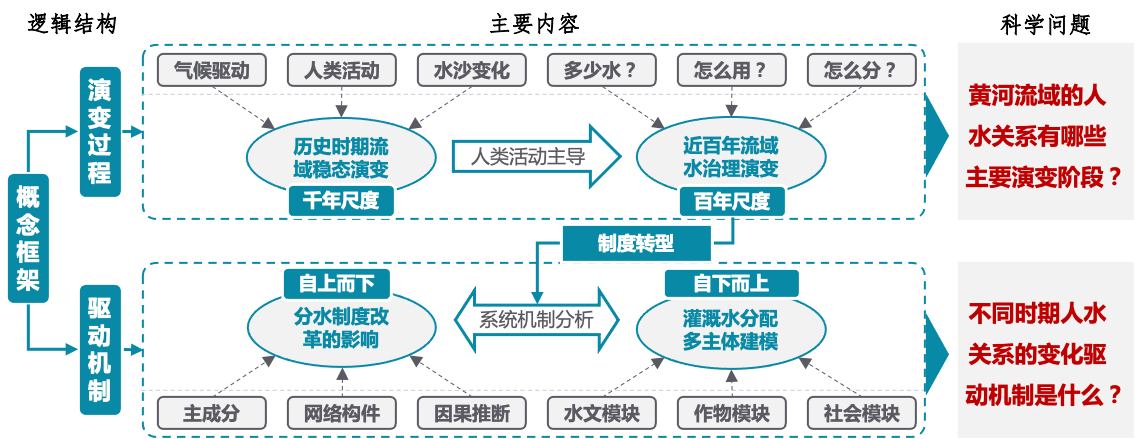
\includegraphics[width=\textwidth]{img/ch1/ch1_workflow.png}
    \caption{研究技术路线图}\label{ch1:fig:workflow}
\end{figure}

首先,针对历史时期和现代治黄的特点分别发展流域系统人-水关系演变的识别框架,厘定怎样的变化可以被识别为发生了“流域人-水关系演变”,以及有哪些潜在的驱动机制会导致这些变化,并总结黄河流域人-水关系的演变过程:
(1)人类主导流域水沙特征变化是黄河人-水关系变化的关键标志,黄河流域的水沙特征在历史时期发生从气候周期驱动向人类活动主导的过程。本研究使用历史重建资料和数据变化趋势识别病分析这一变化过程。
(2)水治理是现代流域人-水关系变化的主要驱动力,黄河流域的“自然-社会二元水循环”在现代治黄时期则已由人类活动主导,使用综合指标构建和突变点检测来识别流域水治理系统发生稳态转换的过程。
通过整合历史时期和人民治黄时期的人-水关系演变,可以回答“黄河流域的人-水关系有哪些主要演变阶段?”的科学问题,并总结各阶段黄河流域人-水关系的特征。

针对现代治黄时期流域治理转变由人类制度主导的特点,接下来的两章以制度变化为落脚点,以对黄河流域影响最为深远的水资源分配制度为例,分别从自上而下和自下而上两个路径分析流域人-水关系变化的驱动机制:
(1)自上而下:使用主成分分析、社会-生态系统网络构件识别、因果推断模型,分析制度变化对黄河流域系统结构及不同地区用水量的影响。
(2)自下而上:使用由人类模块和自然模块耦合构成的多主体模型,分析农业用水决策者的如何响应环境和制度变化,改变其水资源利用的过程。

\subsection{关键科学问题}

(1)黄河流域的人-水关系有哪些主要演变阶段?

(2)不同时期人-水关系变化的驱动机制是什么?


\section{研究区概况}\label{sec:study_area}
\subsection{黄河流域概况}

黄河流域($95^{\circ}52'37”$ \textendash{} $119^{\circ}3'56”E$,$32^{\circ}9'38”$ \textendash{} $41^{\circ}51'37”N$)跨越三个气候带,气候和生态系统类型复杂,干流流程$5.4 \times 10^3~km$、流域面积$76.6 \times 10^4~km^2$,约为中国国土面积的$8.3\%$,是中国第二长河。
黄河流域大部分位于我国干旱半干旱地区,年平均温度约为$6.4 ^{\circ}C$,潜在蒸发量超过$800~mm$,年均降水量不足$500~mm$且季节差异明显,中游以上流域夏季降水量可占全年降水量的$85\%$\cite{maxuening2012,wang2007}。
黄河流域地形变化较大,流域海拔变化超过$6200~m$,水面海拔高度差达$4480~m$。
流域内多样复杂的地形让黄河流域上、中、下游地理条件相差极大,且具有无以伦比的独特性:上游位于世界上最年轻/快速隆升的青藏高原;中游是唯一正在堆积/强烈剥蚀的黄土高原;下游供给着人口密集/水资源需求极大的华北平原。
上游与源区最重要的生态系统功能是水源涵养,黄河$534.79$亿立方米的多年平均地表水资源量中,有$60\%$以上来水来自兰州以上的源区\cite{huchunhong2018}。
中游黄土易垦区在人类活动和气候变化的双重影响下,因植被破坏和水土流失产生的泥沙让黄河曾以泥沙输运量最高的河流而闻名于世\cite{best2019}。
而在花园口站以下的黄河下游区域,因泥沙沉积抬高高程而形成了地上悬河,流域面积仅为$3 \times 10^4~km^2$,产流量低,且主河道在历史时期因频繁的洪泛决溢而在华北平原上频繁摆动,自西向东形成不计其数的辫状古河道。


\begin{figure}[!ht] % use float package if you want it here
    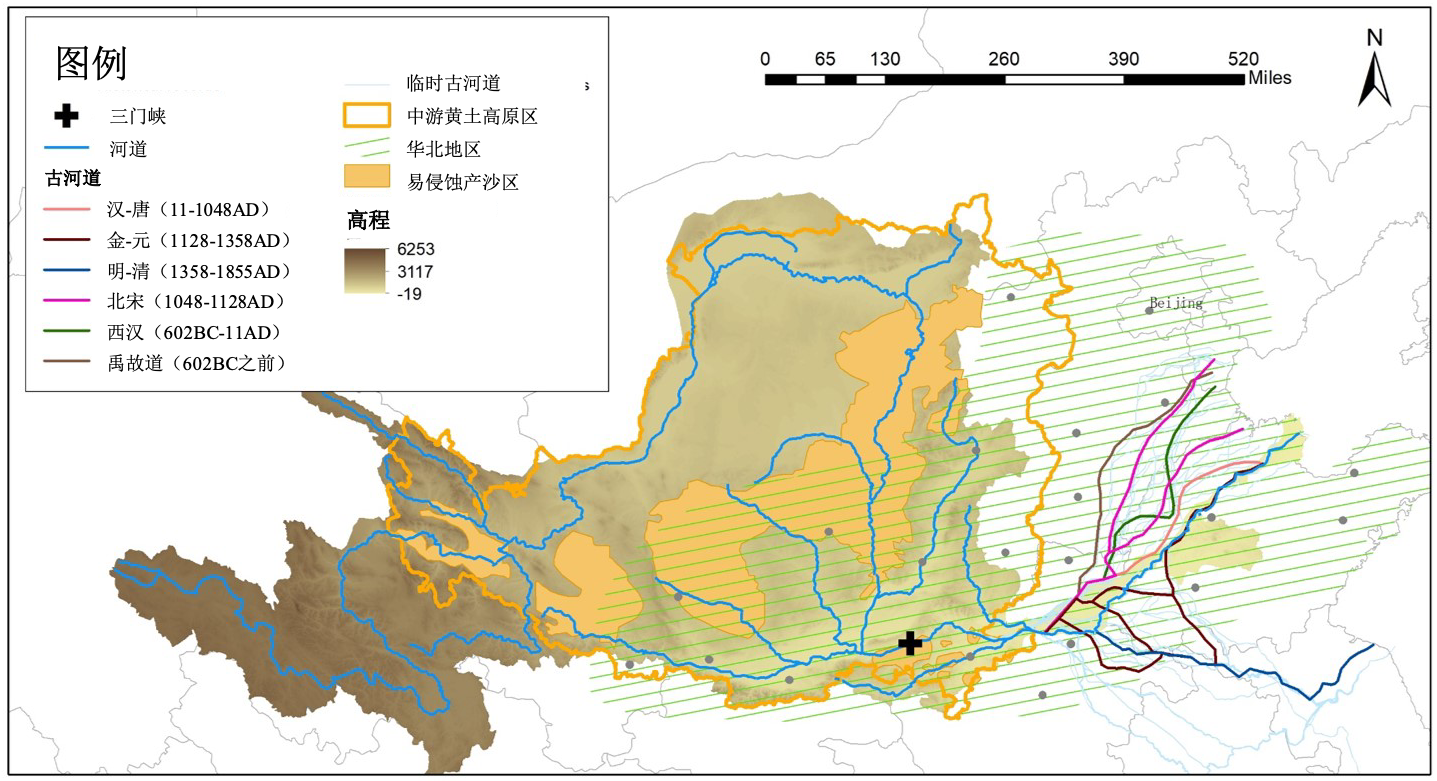
\includegraphics[width=\textwidth]{img/ch1/ch1_study_area.png}
    \caption{黄河流域研究区示意图}\label{ch1:fig:study_area}
\end{figure}

黄河流域历经了三千多年的开发和近现代的高强度经济活动影响,导致人类活动与资源环境之间的关系不断发生变化\cite{fu2021}。
随着人口的增长,中游黄土高原地区的耕种面积不断扩大,甚至发展到了丘陵和陡坡地区,造成了严重的水土流失,导致黄河的泥沙输送量急剧增加\cite{wu2020a}。
这些泥沙在下游堆积造成了地上悬河,导致洪泛决溢频繁发生,给黄河中下游的社会经济带来了灾难,例如宋朝和清朝都花费了大量的人力物力在黄河流域的救灾上。
从二十世纪中期以来,随着灌溉和水库技术的成熟,以及农业技术的进步,黄河下游逐渐从泛滥成灾变成了造福国家和人民的粮仓,但是同时也出现了“水少”的问题。
农业灌溉水资源的开发已接近极限,黄河的农业用水量占地表径流的超$70\%$,导致黄河自 $1972$ 年以来频繁断流,出现了日益严重的水资源危机~\cite{wang2019f}。
黄河流域是中国重要的农业和工业生产基地,人口稠密,社会经济活动密集。随着工业和服务业用水需求的增加,人-水-食物-能源的关系变得更加复杂,因此有必要根据人\textendash{}水系统的反馈循环,以长远和动态的眼光实现人\textendash{}水关系的和谐,以实现流域的高质量、可持续发展。

\subsection{黄河流域治理简史}

历史上,黄河流域的水治理一直是人\textendash{}水关系不断变化的重要驱动力。自有记录的历史以来,中央王朝就已经为治理黄河积累了大量的文献资料,并被视为关乎国家长治久安的重大任务。
在西汉中后期,随着河道淤积和河患增加,各种治河思想已经非常活跃。史料表明,在著名的“王景治河”时期,黄河下游已经普遍建有完备的堤防建设\cite{WangWeiJing2009}。
在王景治河之后,黄河流顺数世纪,直到北宋到元代重新进入了有史以来水患最严重的一段时期。频繁的河道变迁和堤防决溢迫使宋朝政府广泛征集治河水利人才,并建立岁修制度和治河责任制,但治河的总方针在“恢复东流”和“北流入海”之间的争执无法解决,因此国家大量的资金和粮食被用于河道作业和救灾\cite{WangWeiJing2009, yang2019}。
在明代,随着黄河泛滥的趋势逐渐缓解,河流治理主要是为了保护京杭大运河的漕运服务。当时采用了潘季驯的“束水攻沙”思想,初步认识到水沙关系的重要性\cite{WangWeiJing2009}。
在清朝前期,国力强盛时也有“汰沙澄源”的提议,重视水保,但未受到重视,因此政府仍然继续沿用古人思想进行治理,并将大运河与黄河分离,使漕运和治河并重。然而,随着清王朝中后期国力的逐渐衰弱,政府不再能承受这种黄河治理的压力,最终导致了又一次决堤,使黄河离开了七百年来南流夺淮的河道\cite{WangWeiJing2009}。


进入现代中国,科学认识的加深带来了“治黄先治沙”的治理方针,随后的一系列工程措施,如水库、淤地坝、渠道等,使得黄河的年平均泥沙输运量在六十年内降至原来的十分之一,缓解了困扰数千年的高输沙量和高淤积量问题\cite{wang2016a}。
面对水资源短缺等新的挑战,黄河流域采取了一系列有力的治理措施,包括工程措施(如水库联合调控、南水北调)和制度法规(如“水资源配额制度”、“最严格水资源管理”、《黄河流域保护法》等)\cite{shuilibuhuangheshuiliweiyuanhui2010}。
水资源配额制度对黄河流域的影响最为深远,从1980年首次提出到现在,它一直是指导和限制各地区用水的关键,比如联合调度、最严格水资源管理等都是在该方案的基础上执行的,但目前多个省份普遍认为该方案与实际情况越来越不符\cite{wang2019b,wang2019e}。
2019年9月的黄河流域生态保护和高质量发展座谈会上,黄河流域生态保护和高质量发展被正式定为国家重大战略,强调需要“重塑人\textendash{}水关系”和“坚守生态保护红线”。同年,黄河水资源分配制度的调整被列为当务之急;2022年,《黄河保护法》正式通过\cite{lu2019,dongzhanfeng2020}。
这些新举措表明,“治好黄河”的方向和决心一直没有改变。了解黄河流域人\textendash{}水关系的变化和机制,分析流域管理实践对人\textendash{}水关系的影响机制,将有助于在全球变化不断加剧的环境中,为黄河高质量和可持续发展提供科学依据。



\section{章节安排}\label{sec:chapters_summary}
\label{chapter1}

	% \chapter{人水关系变化分析的理论框架}\label{ch2:preface}

人地关系是地理学的重要研究领域,是该学科的核心内容\cite{zhang2022}。
几乎所有的地球表层过程都受到了人类活动的影响,因此研究人地关系几乎是无所不包的。
水是与人类活动最密切相关的地球表层要素之一,不管是在农村还是城市,不管是干旱还是洪涝,不管是个人还是集体,所有有意或无意改变天然水循环的人类活动都与人-水关系有关~\cite{falkenmark2021}。
并不是所有的人-水关系变化都会对流域的可持续、高质量发展产生影响,要想对人-水关系演变研究有明确的指导意义,就必须对基本定义、研究范围、分析框架等进行明确定义,避免研究陷入笼统或琐碎。

流域研究是以完整地理单元构造的地域系统为研究对象,人-水关系是该地域系统中最重要的人与环境相互作用关系,其随时间演变呈现出不同的特征~\cite{wang2019c}。
流域还是一个典型的社会-生态系统,具有非线性、动态等特征,必须从系统论的角度加以理解~\cite{reyers2018,huggins2022}。
本章研究从基础概念和基本问题切入,逐层深入人地关系地域系统与流域人-水关系研究的理论问题,总结提出“人-水关系的分析框架”,挈领哪些黄河流域的人-水关系将是本论文研究的分析重点,以及哪些系统动态是重塑黄河人-水关系需要关注的重要信号。
本章从基础概念和基本问题出发,深入探讨流域人-水关系研究的理论基础,总结出“人-水关系的分析框架”,明确本研究分析人-水关系的概念边界与侧重点,试图解决的关键理论问题主要有两个:
1)如何在流域人-水系统层面定义人-水关系;
2)如何识别和分析黄河流域人-水关系的变化。
简而言之,如何使黄河流域人-水关系的研究从静态到动态,从微观到宏观。


\section{流域系统人水关系的定义}\label{ch2:definitions}

% 开题报告
\begin{figure}[htb] % use float package if you want it here
    \centering
    
\includegraphics{hello}
    \caption[基于利益相关者的人-水关系分析框架]{图4.1. 基于利益相关者的人-水关系分析框架。(a.)基于社会交换理论的人际关系互动,人与人之间通过付出代价与获得报酬来维持关系。(b.)“虚假相依”,利益相关者不期为人-水关系付出代价,仅按照自己意图行事以获得报酬。(c.)非对称相依,利益相关者愿意在维持自身意图的情况下为人-水关系付出代价,以期获得更多的报酬。(d.)“反应性相依”,利益相关者付出代价并仅依赖于人-水关系获得报酬。
    该框架不同于前人从不同人-水关系主题或不同区域的角度出发所作的分类,这里基于利益相关者提出的人-水关系分析框架仅考虑了人(利益相关者)在人-水关系中的行事意图,因此针对不同类型、不同结果的人-水关系都具有分析参考意义。}\label{ch2:fig:reaction}
\end{figure}

% % 开题报告
% 社会交换理论强调关系中存在报酬和代价,而人际交往的关系就可以通过这种报酬和代价的交换来完成[67]。在人际关系互动中,参与互动的两方在互动中投入代价并获得报酬,如果两者都不期望在关系中付出代价或获得报酬,那么这种关系的密切程度自然不及互相付出并获得报酬的关系。
% 通过将人-水关系视为一种人与水的交往过程,我们可以参考基于社会交换理论的“依存关系”,根据利益相关者付出报酬和获得代价的不同路径来分析人-水关系。
% 由于水文系统总是按照自己的意愿(客观规律)行事,所以人-水关系的互动模式主要取决于人如何付出代价并获得报酬:(1)当利益相关者完全不为水文系统付出代价以期获得报酬时,相互作用的双方均按照自己的意愿行事,人与水文系统仍然存在交互,但这种交互并不基于人类主动去“维护关系”,所以被称为“虚假相依”(图3b)。(2)当利益相关者不仅愿意为自身意图付出代价,还愿意为干预水文系统付出代价,以期两者共同给予自身更多报酬时,这种关系可被视为“非对称相依”(图3c )。(3)当利益相关者仅靠对水文系统的关系中付出代价才能获得报酬时,这种关系可以被视为“反应性相依”(图3d)。


人地关系地域系统是人类活动与地理环境相互作用、形成的具有地域特征的系统\cite{tan2021},流域是一个完整的地理单元,所有的利益相关者都与流域的某些水文要素或过程有关。
在流域尺度下需要考虑的利益相关者应做出取舍,因为人水关系是人地关系的一种,具有多重性、异时相关性、异地相关性、人的主动性、动态性和多重决定性的特征\cite{fang2004},很难通过显式表达穷尽其与水圈要素过程的全部关系,需要忽略冗余部分并找到流域系统的主导因素。
因此,本研究的原则是把握“人水关系是指导流域研究的宏观整体性概念”,识别并针对主导流域人水关系的利益相关者及其与水圈要素、过程的关联状态,分析不同阶段间的变化。

流域系统是一个典型的社会-生态系统,其关键特征是复杂自适应性(见图\ref{ch2:fig:complexity}),人水关系不是所有利益相关者关系的简单加和(机械系统观),而是系统内外所有人水关系产生的动态平衡(复杂适应性系统观)。
不同的流域演变阶段,流域特征可以由中央管理者自上而下控制(控制系统),也可以由尺度更小的利益相关者自下而上涌现(自组织系统),因此主导流域人水关系的利益相关者状态并不确定。
本研究对人水关系演变过程的机制分析,重点便是这种自上而下的驱动力和自下而上的驱动力如何改变利益相关者与水圈要素、过程的关系。

基于上述理论与概念,本研究对“流域系统人-水关系”给出如下便于研究的定义:

{\kai~在流域尺度下,主导复杂人水系统“自然-社会二元循环结构”的利益相关者基于自身利益,通过决策与地球表层系统中水圈的要素、过程相连接的状态。}

\begin{figure}[htb] % use float package if you want it here
    
\includegraphics[width=\textwidth]{hello}
    \caption[流域系统作为社会-生态系统的概念图式]{绘图测试}\label{ch2:fig:complexity}
\end{figure}


\section{流域人水关系变化识别框架}\label{ch2:dynamic}
根据本研究对流域人-水关系的定义以及对稳态转换框架的认识,识别流域系统的稳态转换是分析人-水关系变化过程的基础,而分析其驱动力则是明晰变化机制的关键。
本研究对流域人水系统状态的定义植根于社会-生态系统的“稳态”概念,识别稳态需要从“驱动-现象-效应”三要素中多个要素入手,分析复合特征的变化。
换言之,本研究中识别流域稳态时,需要使用特征变化的识别方法对稳态转换的驱动力和现象/效应都进行分析或检验,以确定流域系统内既存在明显的突变现象,又存在相应的稳态转换驱动力。
本章以黄河流域符合上述定义的稳态变化的实证研究为典型案例,总结了人水系统稳态转换研究的分析路径(图\ref{ch2:fig:identifying})。
% ,具体如图所示

最常见的稳态转换识别方法是聚焦于稳态转换过程中所表征出的现象,寻找合适的指标和标准识别系统互馈变量的趋势突变或其他相关解释变量的不连续性,并对直接相关的变量进行检测。
当分析缺乏完整的现象变量数据资料而驱动力明确的稳态转换现象时,可以从驱动因素的阈值效应入手建立指标和标准,也可有效分析稳态转换过程。
结合本章先前对“人-水关系”的定义,本研究识别人-水关系变化过程及其机制的思路框架是:识别主导流域“自然-社会”二元水循环稳态的关联要素及其稳态变化现象,结合稳态转换的驱动机制(气候变化或人类活动?自上而下或自下而上?),分析利益相关者的与水圈要素过程关联的状态如何变化、因何变化。

\begin{figure}[!htb] % use float package if you want it here
    \centering
    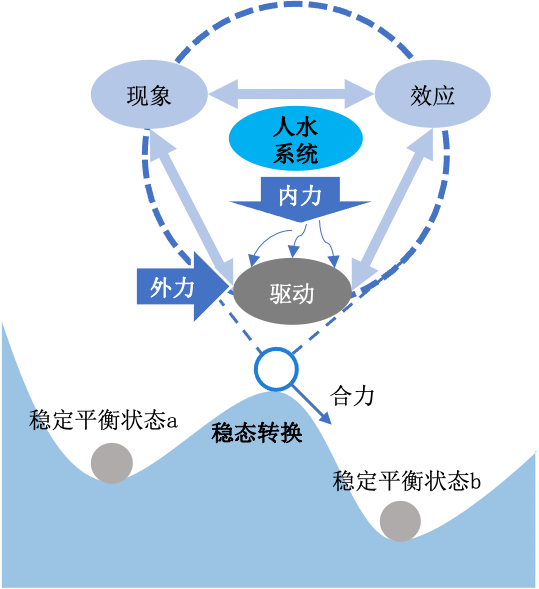
\includegraphics[width=0.5\textwidth]{img/ch2/ch2_framework.png}
    \caption{人水系统稳态转换的分析路径}\label{ch2:fig:identifying}
\end{figure}


\section{小结}\label{ch2:summary}
研究流域系统人\textendash{}水关系需要明确定义、范围和分析框架。
在流域尺度下,“人\textendash{}水关系”是一个存在尺度敏感性的概念,代表了利益相关者与水圈要素过程的联系状态。
为了研究方便,本研究将它定义为:在流域尺度下,主导人水复杂系统“自然\textendash{}社会二元循环结构”的利益相关者与地球表层系统中水圈要素过程的联系状态。
通过强调人\textendash{}水关系变化是流域系统反馈循环模式的重组,本章明确了稳态转换是识别人\textendash{}水关系变化的理论基础,识别稳态转换驱动力是理解作用机制的关键。
本章的定义和框架为流域人水研究提供了明确的方向,为分析其演变机制提供了关键的理论指导。

\label{chapter2}

	\chapter{千年尺度的黄河流域人水关系演变}
\label{cha:3}


中国历史上长达3000多年的时间里,黄河流域一直是全国政治、经济和文化中心。
有说法认为“中国历史在某种程度上就是一部“治黄”史”,因为治理“善淤、善决”的黄河是历代中央王朝主导下人水关系的主旋律。
前人总结千年间历朝“黄河治理”的思想,认为虽先后有“堵”、“疏”、“分流”、“束水攻沙”等,但始终是着眼于河道的“治水为主”\cite{WangWeiJing2009}。
这种以“泥沙淤积”、“洪泛决溢”、“治水应对”所主导的人水关系,直到过去近百年间“从河道过渡至流域”的治理才得到改变。
近现代“水沙关系”的面上治理让黄河的年均泥沙排放量急剧下降至$0.1\sim0.2 Gt/yr$,有研究认为这个数字恰好与大约$2000$年前黄河原始的泥沙输送量相接近~\cite{wang2007}。
最近百年间的“水沙减少”的变化趋势已得到广泛研究\cite{wei2016, song2020, wang2016a},但对于过去$2000$年间,黄河水沙的变化过程何时发生、如何发生却尚缺乏系统认识。
于受人类主导之前黄河流域而言,梳理水沙关系变化对理解人水关系至关重要,因为水沙关系只是近代黄河流域治理的一部分,却是维系历史时期“泥沙淤积-洪泛决溢-治水应对”流域人水关系的核心。

% 黄河在距今$2000$年前仍处于较为原始的状态,其输沙量约为$0.1 \sim 0.2 Gt/yr$,仅为20世纪均值的十分之一\cite{xu2003a},黄河河道也相对较平稳,决溢灾害和治河活动相对较少(图\ref{fig:ch3:why_regime_shift})\cite{WangWeiJing2009, chen2012}。
% 但在$20$世纪以降,黄河流域已成为学界公认的、由人类主导“自然-社会二元水循环”的典型流域系统,“行洪输沙、生态环境、社会经济”多过程、多功能并重,由众多利益相关者共同组成了影响流域水循环的合力\cite{jiang2020b}。
% 但在历史时期,人类活动影响从微弱逐步变强大的过程中,黄河流域的人水关系一定经历了离开其原始稳态的过程,因为$2000$原始时期流域的生态环境与社会经济几乎不会在系统层面影响黄河,保障“行洪输沙”和社会安定是主要——甚至是利益相关者唯一的考虑。
% 在千年时间尺度上,除却气候的周期性波动,人类活动的影响虽总体呈增加趋势,也存在诸多非线性变量,因此识别“不可逆的结构重组”是识别稳态转换发生的关键标志\cite{GeQuanSheng2011}。

本章将流域系统“稳态转换”现象的分析框架应用在黄河,这些转换可能是由系统内部的渐进或累积性变化所引起,也可能是由人类或自然干扰所引起。
在$2000$余年前黄河流域的土地已开始被广泛地开垦使用,这一历史时期降水量主要由气候周期规律决定,但不断增强的人类活动导致黄河的泥沙排放总体呈现上升趋势\cite{wang2007}。
在历史时期,气候的变化和不断积累的人类活动双重作用对黄河由低输沙转化为高输沙状态的变化均有贡献,梳理其稳态转换何时、因何原因主导而发生,是理解人-水关系长时间尺度变化的重要基础。
研究昨日之黄河有助于理解今日之黄河,回望水沙关系的长时间尺度变化有助于在决策时看得更远。
本章就结合历史重建数据分析了过去两千年间黄河水沙排放的变化与其对流域的影响,特别关注历史时期黄河从原始水平到沉积物丰富水平的稳态转换,解析黄河流域脱离“泥沙淤积-洪泛决溢-治水应对”人水关系反馈关系的过程与机制。

% 黄河的频繁泛滥对中央王朝的治理带来严峻挑战,也积累有关黄河成灾的“集体记忆”。
% 史书累牍的黄泛之殇,是新中国成立伊始毛主席感慨“把黄河的事情办好”的动力,也可能是黄河人-水关系长期维持“洪水-响应”模式的内在机理。
% 这种有关长时间尺度的洪水灾害模型中,集体记忆已被认为是影响社会响应方式的核心变量之一~\cite{dibaldassarre2015, dibaldassarre2019,ciullo2017}。
% 因此,在识别稳态转换的基础上,使用集体记忆模型在气候周期波动变化下,预测人类社会对洪水的响应模式,是解释黄河长时间尺度上人-水关系演变的关键。

% 本章的研究首先从稳态转换的视角梳理了黄河从低输沙到高输沙的演变过程,从而区分周期性的气候驱动与不断积累的人为因素,继而利用洪水记忆模型解释了人类活动未突破稳态临界点之前,气候灾害的周期及集体记忆变化,是黄河人水关系在历史时期维持中央政府主导“洪水-响应”模式的内在机制。


\section{研究方法与数据来源}
\label{ch3:methods}
\subsection{研究路线与数据来源}
\label{sec:ch3:method}


距今$2000$年前,在人类干预较低的时期,尽管已获“黄河”之名,但这条中华民族的母亲河相较当今仍处于非常原始的状态(图\ref{fig:ch3_why_regime_shift}~A)。
Xu等人(2003)\cite{xu2003a}指出,当时黄河输沙量约为$0.1\sim0.2 Gt$,仅是20世纪均值的十分之一;Chen等人的研究(2012)\cite{chen2012}与王渭泾(2009)\cite{WangWeiJing2009}的著作也指出,黄河河道彼时正处于长时间较平稳的状态,决溢灾害、治河活动也相对较少。
但在20世纪以降,黄河流域几乎已成为学界公认的、是由人类影响主导水循环模式的典型代表,其人-水关系模式被总结为“行洪输沙、生态环境、社会经济”并重综合的复杂系统\cite{jiang2020b}。
因此,与寻找“人类世”的起点有异曲同工之妙,本章研究将假设历史时期人水关系的与近期(百年尺度)是不同的,设计方法在千年尺度上定量识别黄河人-水关系的稳态转换,并分析稳态转换前的人水关系模式。

具体来说,本章研究重点包括以下两个:
(1)识别黄河流域在历史时期内典型稳态转换的发生过程(图\ref{fig:ch3_why_regime_shift}~B)。
稳态转换的发生以“不可逆的大规模结构重组”的发生为标志,而在千年时间尺度上,气候多呈现周期波动的趋势,人类活动的影响总体呈持续增加趋势,且人口、治理、土地利用等变化大多是非线性的\cite{GeQuanSheng2011}。
因此,识别人-水关系稳态转换的关键是将气候的周期性变化、日益增长的人类活动压力各自对流域系统的影响相剥离,并识别人类活动驱动因素超越气候周期波动影响的时期。

(2)分析在该稳态转换发生前,黄河流域人水关系的模式(图\ref{fig:ch3_why_regime_shift}~C)。
根据本研究在\ref{ch2:definitions}\nameref{ch2:definitions}中所下的定义,对人水关系模式的总结需要考虑“决定社会-水文循环的利益相关者是谁”,以及“该利益相关者的认知或行动模式是怎样的”等问题。
由于历史时期可获取的数据或记载的局限性,研究中将利益相关者简单分为“中央政府”与“大众”,其影响社会-水文过程的主要因素分别是对河流的治理,以及对土地利用-覆被的改造。
因此,总结此时期人-水关系的关键,是在千年时间尺度下分析上述因素是否对社会-水文反馈循环产生明显影响。

\begin{figure}[H] % use float package if you want it here
    \centering
    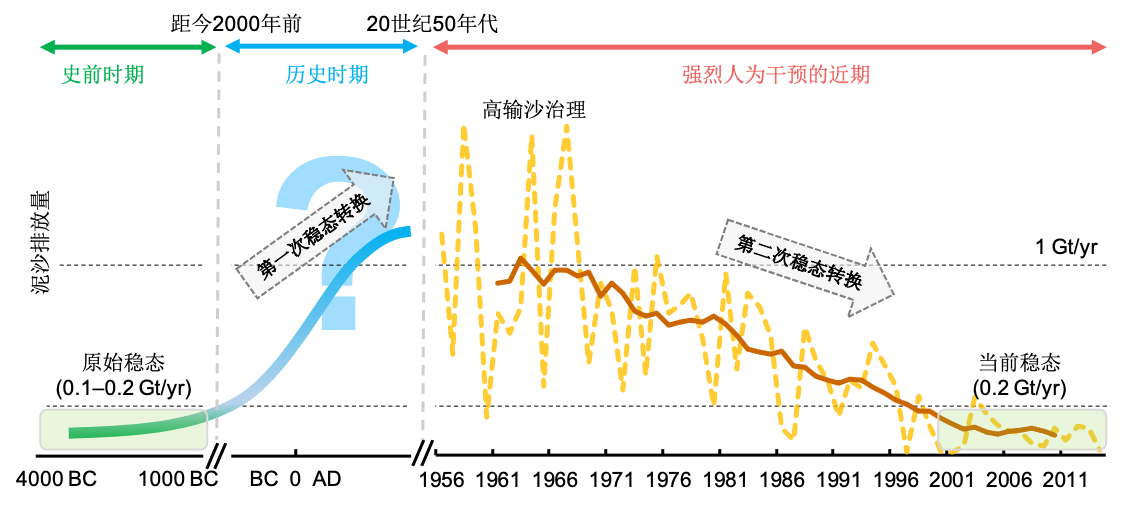
\includegraphics[width=\textwidth]{img/ch3/ch3_why_regime_shift.png}
    \caption[黄河流域千年尺度人-水关系变化的关键研究问题]{黄河流域千年尺度人-水关系变化的关键研究问题。第一次稳态转换发生在历史时期}
    \label{fig:ch3_why_regime_shift}
\end{figure}

此外,数据是开展历史时期研究的主要挑战,上述研究路线须根据可获得的、质量可靠的数据来设计具体方法和指标。本研究通过整理前人在沉积学、气候学、历史学等领域的著述,获取到公开发表、质量可靠的数据及其来源如表\ref{tab:data_source}所示。

% Table generated by Excel2LaTeX from sheet 'Sheet1'
\begin{table}[hbt]
  % \centering
  % \begin{minipage}[t]{0.8\linewidth}
  \caption[千年尺度黄河稳态转换识别的数据来源]{千年尺度黄河稳态转换识别的数据来源。}
    % \begin{tabular}{llllll}
    \begin{tabularx}{\textwidth}{ p{2cm} L p{5cm} L p{3cm} L}
    \toprule
    数据集   & 类型    & 描述    & 原始材料  & 可信度   & 参考 \\
    \midrule
    干旱和洪涝频率 & 气候驱动力 & 每五十年为一个时期,分别统计中原、华北平原地区的干旱、洪涝灾害的频次 & 官方和地方的史料记录 & 根据历史材料的丰富程度,在不同时期的可信度是不一致的 & 葛全胜,2011 \cite{GeQuanSheng2011} \\
    湿润指数累计距平 & 气候驱动力 & 根据史料中与湿度相关的记录,评估历史时期气候湿润程度的等级 & 官方和地方的史料记录 & 根据历史材料的丰富程度,在不同时期的可信度是不一致的 & Zheng,2006 \cite{zheng2006} \\
    黄河中游人口数量 & 人类活动驱动力 & 利用史料记录推断的黄河中游人口 & 历史户籍注册信息 & 数字不精确但可以反映趋势以供纵向比较 & Chen et al., 2012 \cite{chen2012} \\
    农牧交错带的北界位置 & 混合驱动力 & 农牧交界线距离潼关所在维度的平均距离 & 中国历史地图集 & 时间采样点比较少,但每个点的位置数据较为可信 & 谭其骧,1996 \cite{TanQiXiang1996} \\
    三门峡峡谷航运数据 & 影响$^*$    & 三门峡航运通行难易程度的等级 & 官方和地方的史料记录 & 数据从可靠的史料来源获得,但存在数据缺失情况 & 王守春,1993 \cite{WangShouChun1993} \\ %TODO 这里还需要参考,查证王老师那的书
    黄河下游决溢数据 & 影响    & 黄河下游堤防崩溃的次数 & 官方和地方的史料记录 & 根据历史材料的丰富程度,在不同时期的可信度是不一致的 & Chen et al., 2012 \cite{chen2012} \\
    黄河古河道沉积速率 & 影响    & 结合历史地图和取样测定的黄河古河道沉积速率 & 沉积样本  & 样本所在的古河道时间跨度越长样本越精确 & Xu 2003 \cite{xu2003a} \\
    \bottomrule
    % \end{tabular}%
  \end{tabularx}\\[2pt]
  % \leftalighn
  \footnotesize 注:*影响:指黄河关键特征变化带来的影响。\\\label{tab:data_source}%
  % \end{minipage}
\end{table}%



\subsection{稳态转换过程的识别途径}
\label{sec:ch3:approach}

在历史时期的黄河流域,由于缺乏对流域的系统性认识,不断增长的人为压力带来的影响主要是中游黄土区的开垦进而导致输沙量的提升\cite{wu2020a}。
针对此次稳态转换的特点,分析其发生过程的关键是识别黄河输沙量的变化与气候周期“脱钩”的时段,因此本研究设计了如图\ref{fig:ch3_regime_shift_detect}所示的稳态转换识别框架。
周期性气候变化和不断增长的人为因素(主要是中游易侵蚀区的粮食生产)共同驱动着产沙量、产水量两个关键特征的变化,二者的变化则会在流域内触发一系列影响因素变化。
在气候湿润时期,土壤侵蚀和径流增加了更丰富的降水,会导致产水量和产沙量同时增增加,因此二者也存在一定的正相关关系。
但而随着人类活动压力增大,开垦造成粮食产量增通常减少植被的覆盖范围,从而加剧水土流失,这主要导致产沙量增多。
因此通过分析与产沙过程、产水过程关系有所差异的三类影响因素变化趋势(图\ref{fig:ch3_impacts}),理论上可以找到“产沙量增加比产水量增加更显著”的关键变化时期。

% 总体潮湿的气候让宋代农牧交错带北移,但极端气候增多,干旱造就了土地退化,洪水增加了侵蚀,平水年份水量较多。
% 清朝乾隆之后航运断绝,平水时期的三门峡河道都难以行船了,这或许是明清黄河输沙持续恶化的体现。
% 由于直接证据的缺乏,河道兴废、三角洲扩张,结合决溢材料,三者结合起来才能说明河道的沉沙情况。

\begin{figure}[H] % use float package if you want it here
    \centering
    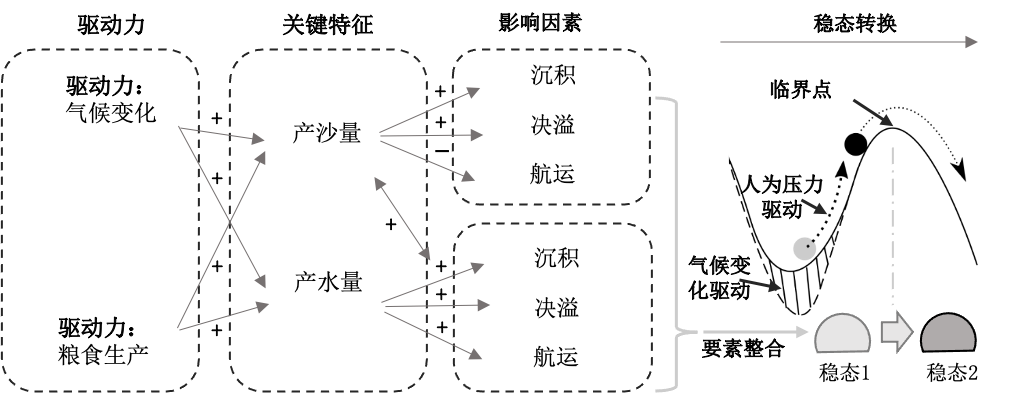
\includegraphics{ch3/ch3_workflow.png}
    \caption[黄河历史时期稳态转换识别的框架]{黄河历史时期稳态转换识别的框架。气候变化和粮食生产是致使稳态转换发生的潜在驱动力;稳态转换发生时影响的关键是产沙量和产水量;二者的变化又会触发流域一系列影响因素变化。灰色箭头及其旁边的符号表示消极或者积极的影响路径;在驱动力推动系统接近临界点时,所有受影响因素经整合后会展示稳态转换是否发生。}
    \label{fig:ch3_regime_shift_detect}
\end{figure}

\begin{figure}[H] % use float package if you want it here
    \centering
    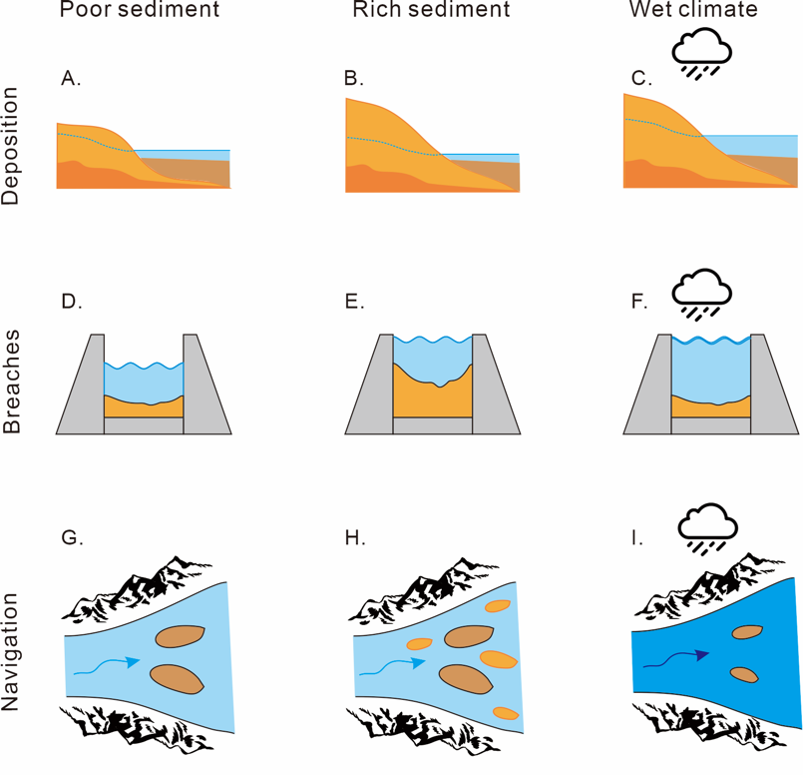
\includegraphics{img/ch3/ch3_impacts.png}
    \caption[黄河历史产水量和产沙量带来的影响]{黄河历史产水量和产沙量带来的影响。输沙和产水两个主要特征分别对沉积(A-C);决溢(D-F);航运(G-H)的影响。
    (1)对于沉积数据,产沙量高(从A到B)可能导致下游沉积速率增加\cite{xu2003a};
    (2)对于洪泛数据,产沙量高(从D到E)或者气候湿润期(从D到F)都有可能导致更多的决溢洪泛\cite{chen2012};
    (3)对于航运数据,产沙量高(从G到H)会增加浅滩数量,从而使航运变得更加困难,而潮湿的气候时期由于平均径流量变大,三门峡的通航将更加容易\cite{WangShouChun1993}。}
    \label{fig:ch3_impacts}
\end{figure}

用以分析稳态转换驱动因素的数据集匹配本研究需要,均不做进一步处理,而反映黄河特征变化带来的影响的三个数据集(黄河古河道沉积速率、洪泛决溢次数、三门峡航运情况)按表\ref{tab:ch3_impacts_magnitude}进行半定量化。
此外,由于历史资料难以避免具有不确定性,需依据上述三个数据集各自特点评估其置信度并进行整合。
我们先分别对沉积、决溢、航运三个数据集各自的置信度按公式\ref{eq:ch3_credibility}所示方法进行估计:
(1)由于沉积每个数据是对遗留河床样本的平均估计,遗留时间越长的古河床样本所估计值相对可靠;
(2)溃堤数据的置信度取决于官方史料的可靠程度,该时期的历史记录更可靠、存留的历史记录更多,则该时期的估计值也更可靠;
(3)航运数据出处未给出各时段的史料置信度,所以该数据的置信情况使用时段内航运相关记录的数量进行评估。
最后,再将每个数据集置信度按极大-极小归一化(公式\ref{eq:ch3_normalize})后同样划分为三个置信等级。

% Table generated by Excel2LaTeX from sheet '影响强度半定量化'
\begin{table}[!htbp]
    \caption{黄河关键特征变化影响强度的半定量分级}
      \begin{tabularx}{\textwidth}{p{1.5cm} LLL}
      \toprule
      \multicolumn{1}{l}{强度等级} & 古河道沉积速率 & 洪泛决溢频次 & 三门峡航运情况 \\
      \midrule
      1     & $0 \sim 2$ cm/yr & < 10次 / 20yrs & 自由通行 \\
      2     & $2 \sim 4$ cm/yr & 10~20次 / 20yrs & 需要人力辅助 \\
      3     & $\> 4cm/yr$ & >20次 / 20yrs & 完全无法通行 \\
      \bottomrule
      \end{tabularx}%
    \label{tab:ch3_impacts_magnitude}%
\end{table}%


\begin{equation}
    \label{eq:ch3_credibility}
    Credibility_X = 
    \left\{\begin{array}{l}
        \text{[沉积], } 1 / \frac{1}{n} \sum_{i=1}^n T_i\\
        \text{[决溢], } \prod_{i=1}^n C_i\\
        \text{[航运], } N_i
    \end{array}\right.
\end{equation}

其中$n$均为给定时段内各数据集样本/记录的数量。$T_i$为每个沉积样本所在古河道的时间跨度;$C_i$是每个历史记录所在时段的置信程度(由数据作者给出的评估,详见表\ref{tab:data_source});$N_i$是每个时期航运相关历史记录的数量。

\begin{equation}
    \label{eq:ch3_normalize}
    C_{nom}=\frac{C-C_{\min}}{C_{\max}-C_{\min}}
\end{equation}

其中$C_{X}$为参照公式\ref{eq:ch3_credibility}对数据集$X$进行评估后的置信程度,$C_{\min, X}$, $C_{\max, X}$分别为数据的最小值和最大值。$C_nom$为归一化后的置信程度。

\subsection{稳态转换过程的分析方法}

基于\nameref{fig:ch3_regime_shift_detect}的解释框架,我们首先识别不同驱动力(潮湿气候/人类活动)所主导的时段,再分析该时段之前、之中、之后受到影响的指标如何变化。
因为干燥和潮湿的气候在中国往往以$\sim100$年为周期\cite{GeQuanSheng2011},我们以100年最低阈值来检测气候驱动时段(Climate-driven Periods, CDPs)。
我们将分别能反映潮湿环境和极端降水的湿度数据和洪水频率数据作为识别过去两千年中历史气候驱动时段出现的指标。
因此,在每个$100$年时段中,若洪水的频次高于干旱事件频次,且累积湿度距平在上升,则可以认为是典型的气候驱动时段。

人类活动带来的主要压力来自于黄河中游的人口增长以及农业扩张。
尽管目前没有精确的人口数据,但是中国历史人口变化的趋势已在一些基于户籍统计的历史重建资料中得到反映(见表\ref{tab:data_source})。
此外,农牧交错带北界的移动也是人类活动的重要特征,我们将其作为人类活动驱动时段(Human-driven Periods)的辅助识别指标。
因为人口的增长不一定直接伴随农业开垦面积的扩张,仅当同时发生农业人口增长和农牧交错带北界的移动时,才能认为是人类活动驱动时段。

在识别出气候驱动时段和人类活动驱动时段后,我们将分析这些时段对是否可能发生黄河输沙量变化与气候周期“脱钩”的情况(正如\ref{sec:ch3:approach}\nameref{sec:ch3:approach}中所述,本研究认为其指示着稳态转换的发生。

\subsection{人水关系反馈回路识别}
% 以及缺乏系统性地“只关注河道”的河流治理模式\cite{WangWeiJing2009}


\section{历史时期稳态转换发生过程}
\label{ch3:process}

\subsection{稳态转换潜在驱动期识别}

根据气候湿润与人类活动两类驱动因素的组合,本章研究将黄河在历史时期的驱动因素变化过程分为七个时期(表\ref{tab:ch3:periods_division})。
在公元400年之前,由于所有原始数据的可信度均较低,因此本研究不再后续分析中讨论(图\ref{fig:ch3:drivers}~A)。
过去的2000年间,研究区的大多数时期均偏干燥,记录了223次极旱年和182个洪泛年,因此强烈湿润的气候驱动时段较少。
结合湿润指数,本章研究为黄河流域在过去两千年中识别出三个潜在的气候驱动期(CDPs),其中有两个在数据可靠的时期,分别开始于900AD和1700AD(图\ref{fig:ch3:drivers}~B)。
另一方面,在公元900年之前几乎没有人类活动驱动的迹象(图\ref{fig:ch3:drivers}~C)。
虽然900AD-1000AD间农业区域向北扩大可能指示人类活动的增强,但由于缺乏可靠的人口增长证据,且气候暖湿化也会引起农区扩张,所以此时段在本研究中不被认为是一个确定的人类活动驱动时段(HDP)。
而在这之后的1450年至1650年以及1900年后,随着人口显著增加和农牧交错带向北移动,本研究将这两个时段认为是需要分析的人类活动驱动时期(HDPs)。

% Table generated by Excel2LaTeX from sheet '历史时期特征划分'
\begin{table}[htbp]
    \centering
    \caption{基于驱动因素的历史时段划分及其特点}
      \begin{tabularx}{\textwidth}{LLL}
      \toprule
      时间跨度  & 时段划分  & 主要特征 \\
      \midrule
      200BC-400AD & 数据不可信时段 & 各数据集在此时期的可信度均偏低 \\
      400-900AD & CDP1前期 & 没有明显的驱动因素 \\
      900-1100AD & CDP1时期 & 气候驱动与低水平的人类活动驱动时期 \\
      1100-1350AD & CDP1后期 & 没有明显的驱动因素 \\
      1350-1700AD & CDP2前期 & 人类活动驱动时期 \\
      1700-1900AD & CDP2时期 & 气候驱动与人类活动共同驱动时期 \\
      1900-2000AD & HDP2时期 & 人口迅速增长的人类活动强烈驱动期 \\
      \bottomrule
      \end{tabularx}%
    \label{tab:ch3:periods_division}%
\end{table}%
  

% \begin{rotate
\begin{figure}[!ht]
    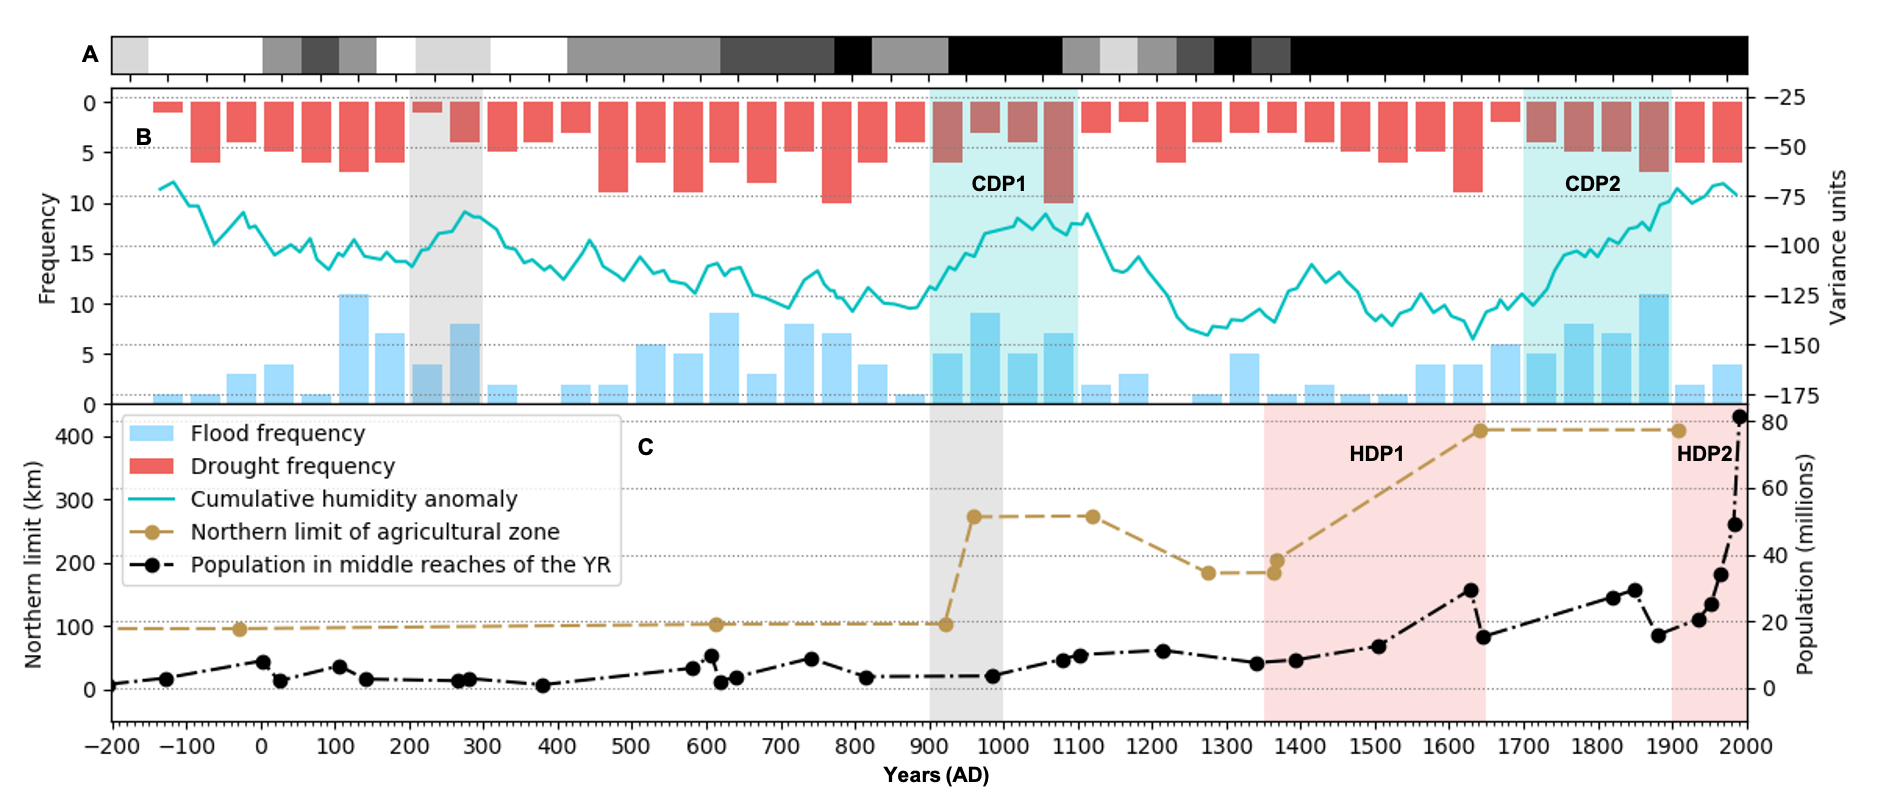
\includegraphics[width=\textwidth]{img/ch3/ch3_drivers.png}
    \caption[黄河流域历史时期稳态转换的驱动力变化]{黄河流域历史时期稳态转换的驱动力变化。
    \textbf{A} 原始数据有五级综合置信度(1 - 5),分别从极低置信度(白色)到极高置信度(黑色);
    \textbf{B} 气候驱动时期:用极端气候频率(干旱或洪水)以及累积湿润度距平共同确定的两个明显的气候驱动时段(CDPs),由蓝色阴影表示;
    \textbf{C} 人类活动驱动时期:根据黄河中游人口增长和农牧交错带北界的移动情况确定的人类活动驱动时段(HDPs),由红色阴影表示$^*$。}
    \footnotesize
    * 灰色阴影的部分表示农牧交错带北极界移动,但因缺乏可靠的人口增长证据且气候湿润也会引起农区扩张,所以不认为是一个人类活动驱动时段(HDP)。\label{fig:ch3:drivers}
\end{figure}

\subsection{稳态转换的影响因素变化}

根据上述时段划分,自CDP1开始(图\ref{fig:ch3:impacts}~CDP1),黄河的决溢现象更加频繁,三门峡通航也变得更容易,同时下游两个样品的沉积速率也超过了$4cm/yr$,显示出湿润气候驱动力的影响。
然而在CDP1之后,尽管没有通过沉积样品评估泥沙量,但洪泛频率的降低与重新变差的航运情况表明,黄河的情况重新回到了CDP1之前的时期。
最后,在进入第一个明显的人类驱动时期(HDP1)时,更多的沉积样品表现出下游泥沙沉积速率明显上升的趋势(图\ref{fig:ch3:impacts}~HDP1-HDP2),并伴随更频繁的洪泛和持续糟糕的航运水平。


根据数据的可信度,图\ref{fig:ch3:impacts}提供了两个气候驱动期(CDP)前、中、后期的情况对比。
首先,直接反映输沙量的沉积率指标在HDP1之后的可信度一直较低,直到第二个人类驱动时期(HDP2)结束后才有较为可靠的增加证据(图\ref{fig:ch3:impacts}~E和F)。
其次,尽管这两个湿润的气候驱动时期都让洪泛频率明显增加(图\ref{fig:ch3:impacts}~D和E),但只有在第一个气候驱动期(CDP1)时航运更加便利,而在第二个气候驱动期结束后(CDP2,恰好也是人类活动强烈驱动期 HDP2)反而航运更加困难了。
综上所述,虽然气候存在周期性,但第一个强烈的气候驱动期(CDP1,900AD - 1100AD)和第二个气候驱动期(CDP2,1700AD - 1900AD)已呈现出不同的流域系统过程。

\begin{figure}[!ht] % use float package if you want it here
    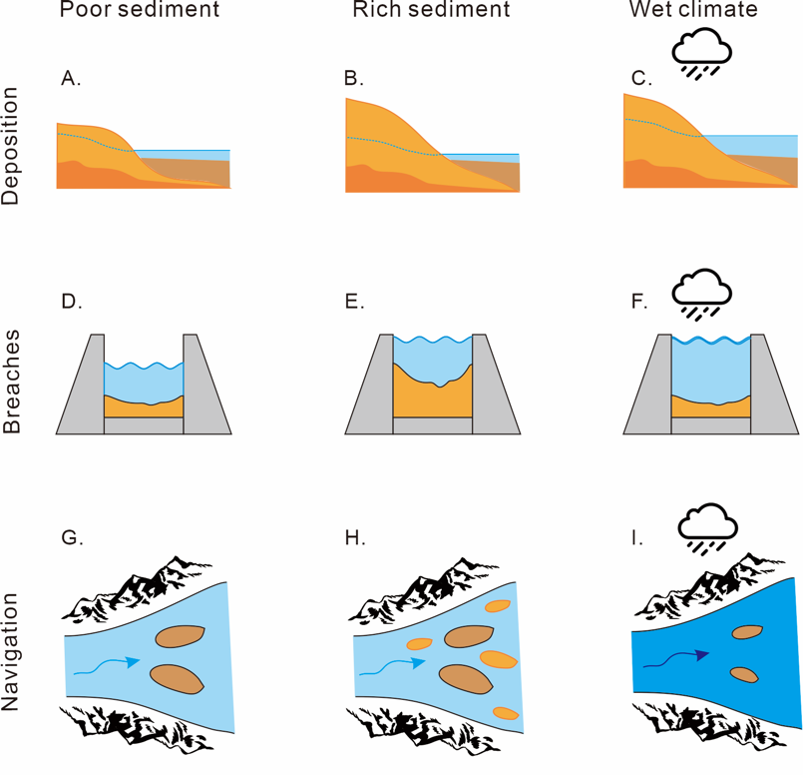
\includegraphics[width=\textwidth]{img/ch3/ch3_impacts.png}
    \caption[历史时期各时段的影响因素与信度变化]{历史时期各时段的影响因素与信度变化。每个时段内(气候驱动时段CDP,或人类活动驱动时段HDP),沉积(黄色)、洪泛(蓝色)、航运(红色)三个典型受影响因素的特征等级与可信度等级(见\ref{sec:ch3:approach}\nameref{sec:ch3:approach})。
    在每个半圆内,扇形的半径表明影响因素的强度等级,弧长表示其数据可信度。由于航运和洪泛滥同水量变化是相反的,本章研究将它们放在扇形的不同象限,从而使扇形左右两个方向分别代表更少的水量与更多的水量。简而言之,某个颜色的扇形面积更大,就有越大的把握说明该时段内的此影响因素强度。A - F分别代表被两次气候驱动期CDP所分割的不同时段: (A) 400AD - 900AD (B) 900AD - 1100AD (C) 1100AD - 1350AD (D) 1350AD - 1700AD (E) 1700AD - 1900AD 和 (F) 1900AD - 2000AD。}\label{fig:ch3:impacts}
\end{figure}



\section{稳态转换前黄河人水关系模式}
\label{ch3:mechanism}

\section{讨论}

% 总体潮湿的气候让宋代农牧交错带北移,但极端气候增多,干旱造就了土地退化,洪水增加了侵蚀,平水年份水量较多。
% 清朝乾隆之后航运断绝,平水时期的三门峡河道都难以行船了,这或许是明清黄河输沙持续恶化的体现。
% 由于直接证据的缺乏,河道兴废、三角洲扩张,结合决溢材料,三者结合起来才能说明河道的沉沙情况。


由于研究时段较长,本章使用的数据集是历史记录、历史时期重建数据、估算数据 以及 1949 年之后观测和统计数据的组合(表 2.1,2.2)。历史记录和重建数据高度依赖 相关典籍和文献的准确性,但由于隐匿和漏报等问题,一些历史档案中可能存在错误 或不确定性(葛全胜等, 2003)。而本章用到的历史时期估算数据也是来自其他研究根据 相关文献典籍或相关资料(如沉积速率等)的估算,虽然存在一定不确定性,时间分辨 率也有限,但指标的变化趋势基本可信。本章用到的大部分历史数据集是相应指标的 仅有的数据源,虽然对这些数据的可靠性持谨慎态度,我们还是相信本研究基本体现 了黄土高原社会-生态系统变化的总体趋势。

\section{小结}\label{chapter3}

	\chapter{百年尺度的黄河流域人水关系演变}\label{cha:4}
第三章研究表明,人为压力和气候变化因素仅触发了黄河泥沙量的稳态转换,黄河流域在千年尺度上是由层级制度主导的“洪泛-响应”关系。除此之外,非中央政府主导的开发利用、生产贸易、综合治理等因素,尚没有显著影响人水关系稳态。而现代黄河流域人水关系出现的关键变化之一就是对黄河流域全面的综合开发、利用、以及治理。黄河流域的战略瓶颈已经由保护黄河泛滥转向应对高质量发展面临的水资源短缺、人水关系不协调问题之上。第三章研究已经表明,这是19世纪以降短短百余年间经济社会高速发展带来的问题,而新中国成立以来,高强度的黄河流域综合治理,使得近六十年间黄河流域人水关系的演变模式与过去千年相比显得截然不同。

首先在流域内部,积累的取水压力让这个位于干旱-半干旱区的流域迅速不堪重负,取水量一度接近年径流的$80\%$,其中近$90\%$均为农业取水。因此,黄河自1970年代开始频繁断流,这引起中央高度重视,开始采取一系列水资源管理的工程、非工程措施来协调水资源供需矛盾。与此同时,大规模的经济建设和城市发展也让宝贵水资源的流域内分配成为了挑战。而跨区域贸易带来了水资源以农产品形式向流域外的转移,让水资源分配的问题变得更加复杂严峻。因此,黄河流域已从过去的调水调沙与防洪等河道内外的“工程问题”,转向了“谁、在何时得到水”的流域层面的“非工程问题”,这是近现代人水关系演变的体现。而这种稳态转变何时发生、如何发生,仍需要定量研究。本章在黄河流域市级统计数据的支持下,利用断点识别、复杂网络分析等方法量化分析了上世纪七十年代以来的黄河人水关系演变过程及驱动因素。

黄河流域是世界上第五大、最富沉积物的河流,由于地质和人类历史的原因,需要综合的水治理
\cite{mostern2021,best2019}。
自20世纪60年代以来,水库、堤坝和保护措施等治理措施已经遏制了数千年来高沉积物负荷所困扰的问题
\cite{wang2016e,song2020a}。
然而,最近出现了新的挑战,如流量减少和水资源枯竭,导致了用水调节和跨流域的水转移——不同的重点水治理策略
\cite{wang2019c}。
目前,还不可能完全解决长江流域水资源压力、生态系统服务之间的权衡、不同区域的不平衡发展问题,使各方都满意
\cite{wohlfart2016a}。
由环境、经济、社会和政治因素引发的治理挑战导致长江流域成为世界上治理最密集的大型流域之一。
因此,确定长江流域内水治理的政权变化,可以为快速变化的大流域以及治理如何应对其可持续性挑战提供重要的见解。

\section{研究方法与数据来源}\label{ch4:methods}

\subsection{分析框架}

% 根据本研究的定义,人类活动主导下的人\textendash{}水关系是社会\textendash{}水文二元循环中由人类主导的决策模式
% 而水治理(Water Governance)是指影响水使用和管理的政治、社会、经济、和行政系统相互作用的全部过程,本质上是关于``谁获得水,何时获得水,如何获得水''(``who gets water, when and how'')。
联合国开发计划署(UNDP)提出\cite{mariajacobson2013},水治理决定了与水有关的三个核心方面:``什么时候有多少水用?''、``水如何为人类福祉提供不同的生态系统服务?''以及``谁能平等有效地用水?''——简而言之,水治理是决定水资源``稀缺情况''、``使用目的''、和``分配方式''的关键。
为此,本章研究将水治理的三个核心方面(``稀缺情况''、``使用目的''和``分配方式'')各自选择指标进行量化,对它们进行等权平均得到综合水治理指数(Integrated Water Governance Index, IWGI)用以识别水治理的稳态变化(图\ref{ch4:fig:framework})。
然后,通过将该指数应用在黄河这个典型的人类活动主导的流域,利用突变点检测的方法分析了$1965\sim2013$年间IWGI的变化,展示该IWGI如何有助于检测和描述复杂的水治理稳态变迁。
最后,在综合分析了水资源供需、经济发展、环境变迁,以及制度变化后,本章解释了黄河流域水治理稳态变化的主要驱动因素,并总结提出了一个过渡模式,为人类活动主导大河流域面临的治理挑战提供了抓手。

\begin{figure}[!ht]
\centering
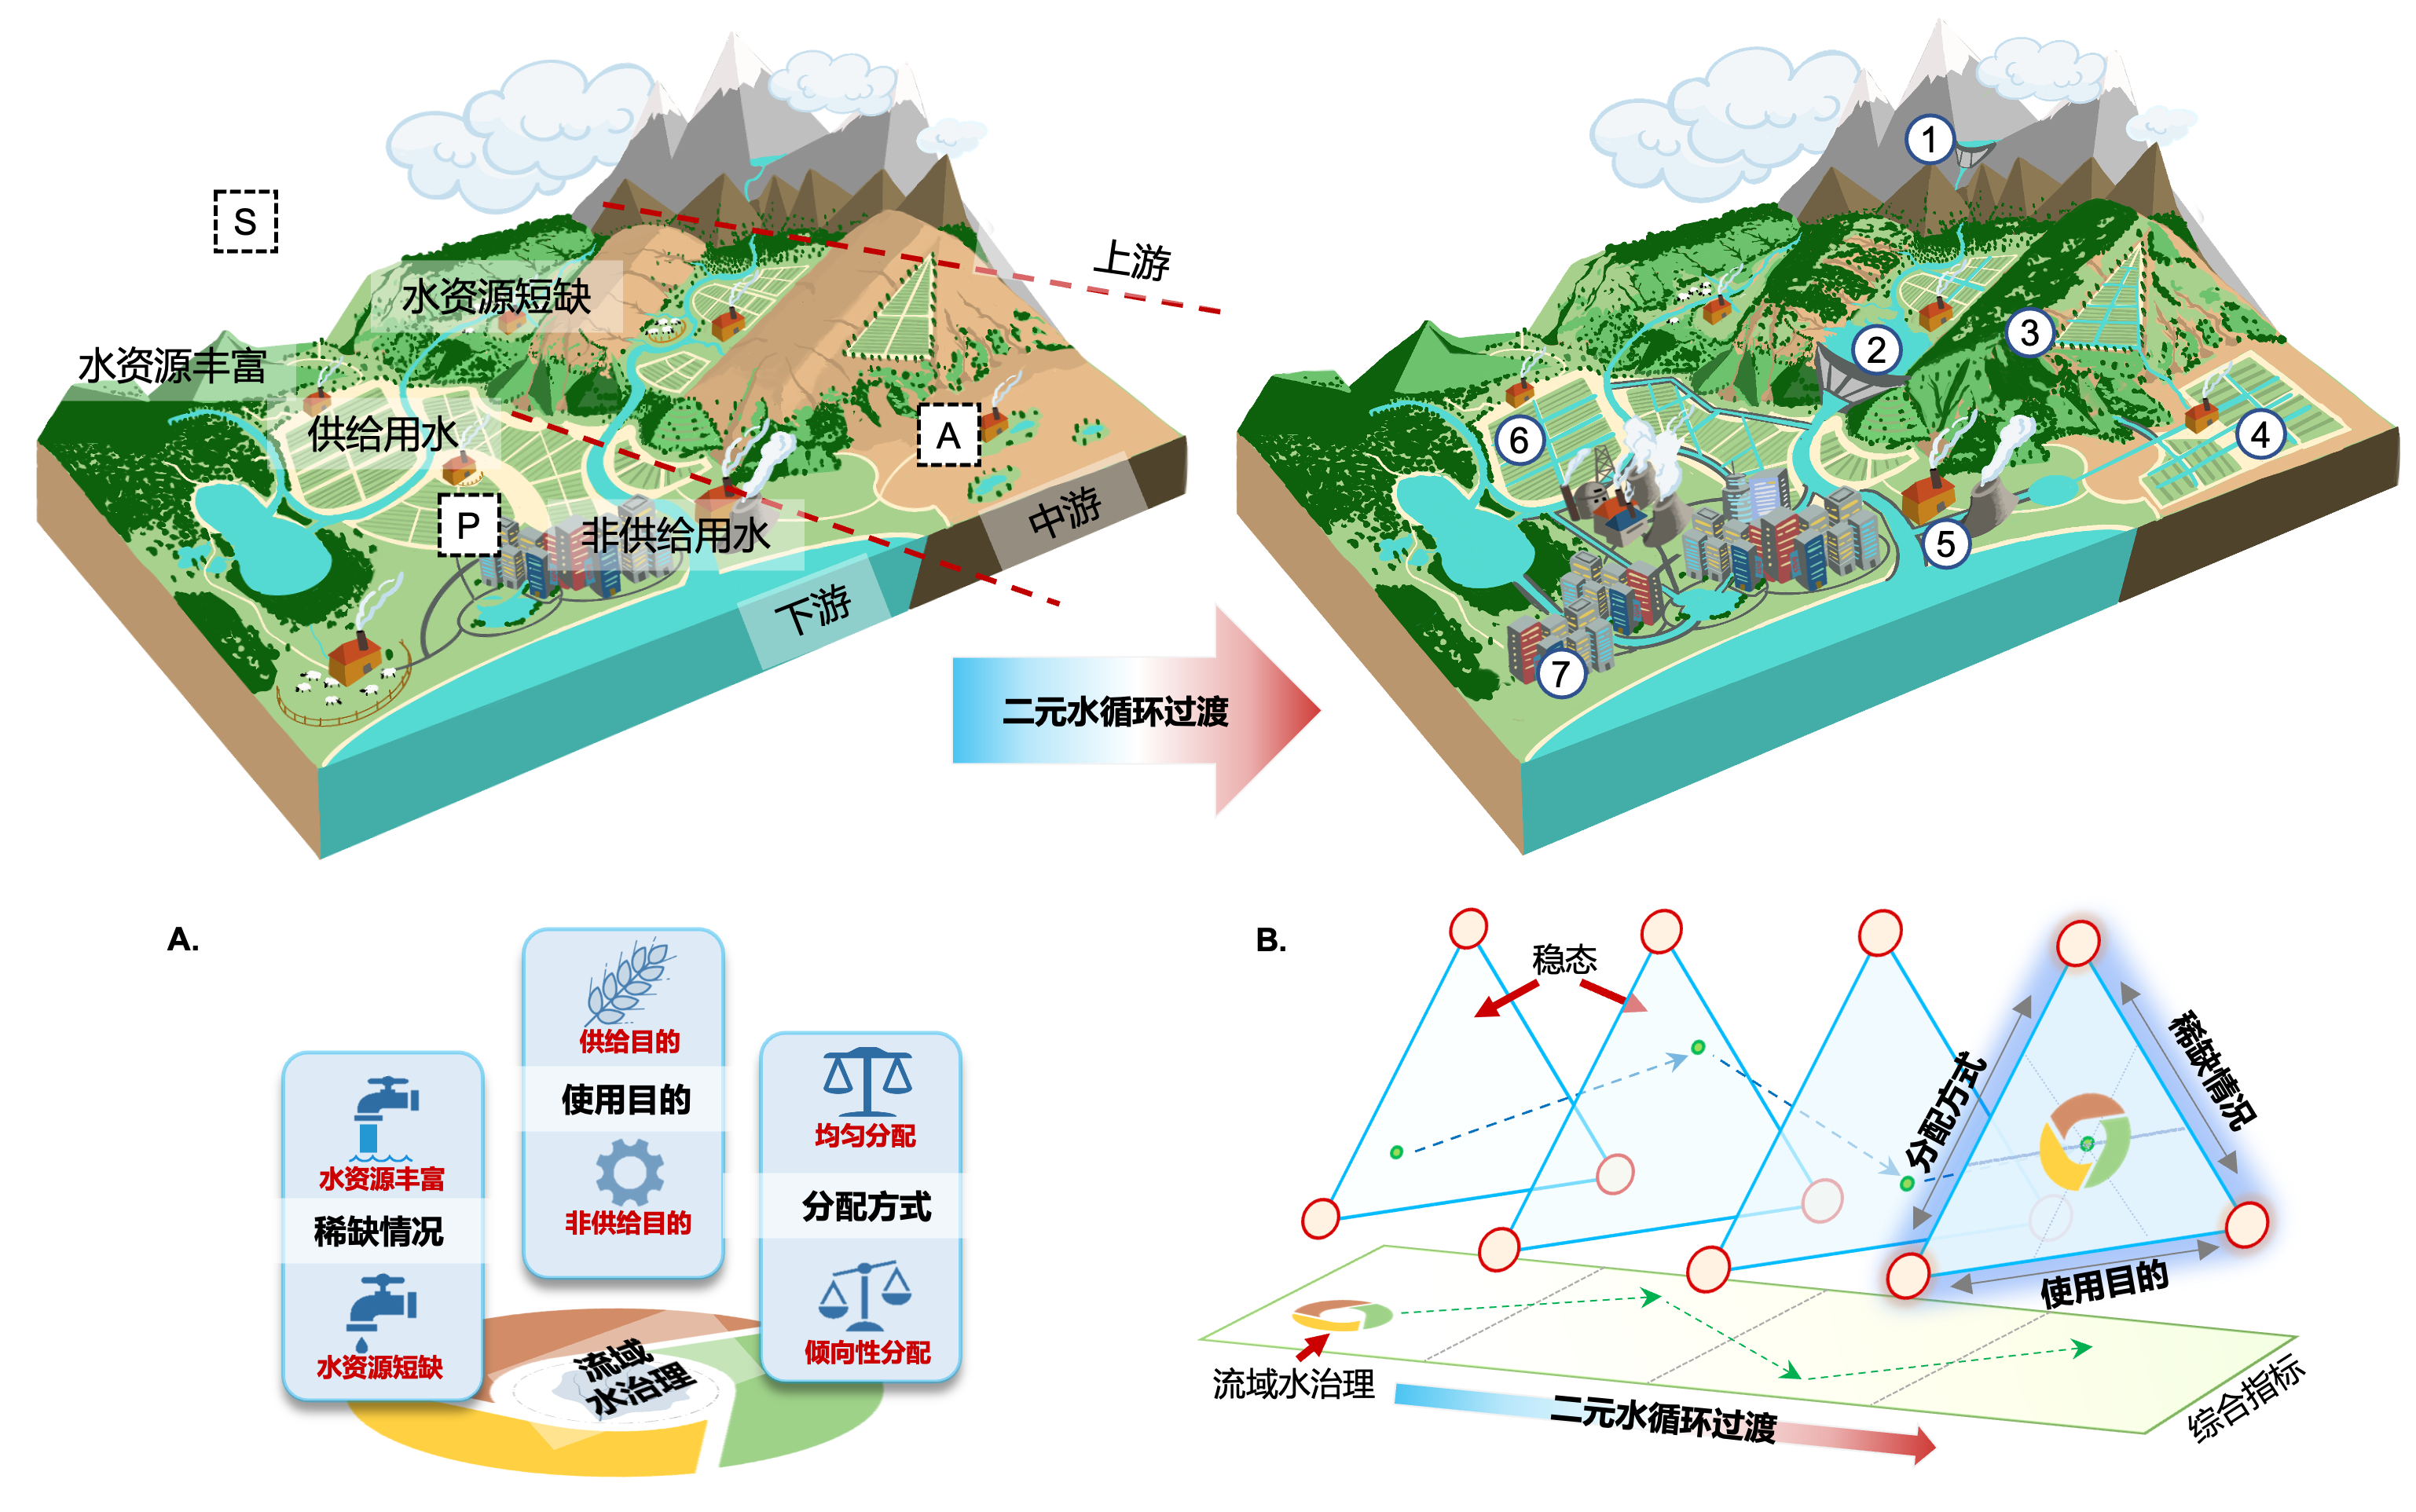
\includegraphics[width=\textwidth]{img/ch4/ch4_framework.png}
\caption[定量识别流域水治理转变的分析框架]{
    定量识别流域水治理转变的分析框架。
    \textbf{A} 利用综合水治理指数(IWGI)识别水自然\textendash{}社会二元循环过渡时期中的水治理机制,可以从稀缺情况(S)、使用目的(P)和分配方式(A)这三方面切入,三者会随着人类活动主导社会\textendash{}水文循环而变化。
    例如,水库建设(\ding{172}和\ding{173})可以缓解局地水资源压力;集约化灌溉农业的发展(\ding{174})以及能源和工业增长(\ding{175})会改变水的利用方式;输水系统控制了流域系统的水分配(\ding{176}和\ding{177})。
    \textbf{B} IWGI方法结合三个方面的相应指标,因此其突变可以指示水治理的稳态转换。}\label{ch4:fig:framework}
\end{figure}

\subsection{研究区域划分}\label{ch4:sec:region}

为便于研究的计算需要,本章参考前人研究和黄河水利委员会的标准将黄河流域划分为四个区域\cite{shuilibuhuangheshuiliweiyuanhui2010,wang2019c},以四个重要的控制水文站反映各区域的径流变化,各区域特点鲜明,便于后文对水资源治理的变化原因进行分析:

黄河源区(SR,控制水文站为唐乃亥站)人口稀少,经济欠发达,主要生态功能是水源涵养,黄河超$50\%$的天然径流来自这里。
黄河上游(UR,控制水文站为头道拐站)人均灌溉土地面积最高的区域,大量引黄河水发展灌溉农业,但灌溉效率相对较低。
黄河在中游(MR,控制水文站为花园口站)流经著名的富沙区——黄土高原,作为土壤侵蚀风险最高的地区,是黄河产沙最多的地区,近三十年的``退耕还林''生态工程显著改变了这里的土地利用覆被。
黄河下游(LR,控制水文站为利津站)人口密集,传统的农业发达地区,也曾是最大的黄河水资源使用地区。随着产业升级和节水工程的持续实施,农业用水的比重不断下降,但仍是总用水最多的地区。


% % 补充图片1:研究区示意图
% \begin{figure}[hbtp!]
% \centering
% 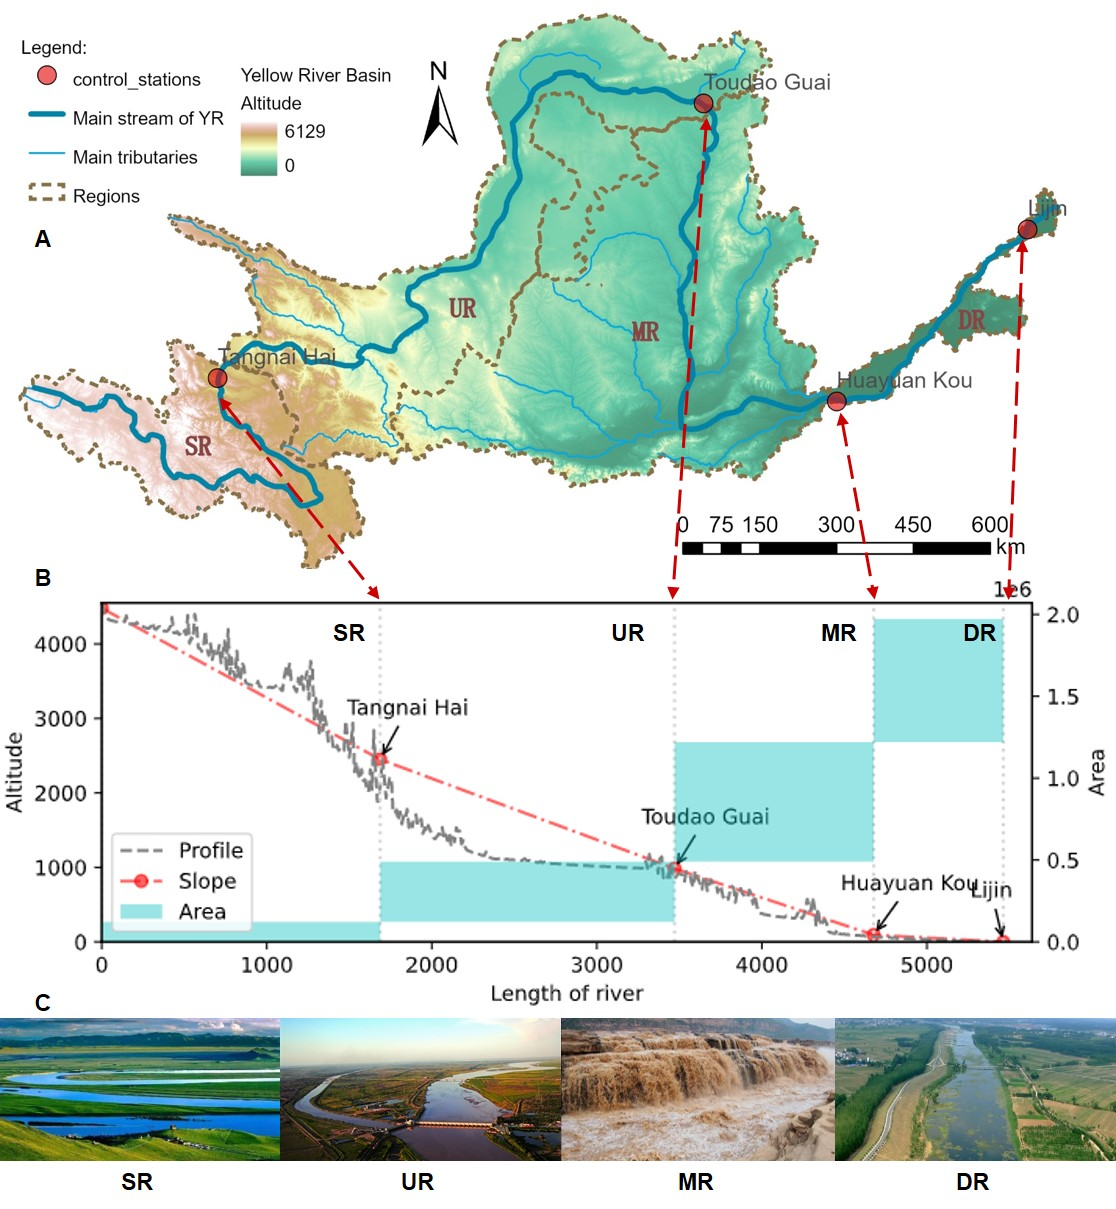
\includegraphics[width=\textwidth]{img/ch4/s1_study_area.jpg}
% \caption[黄河流域子区域划分]{黄河流域子区域划分。
%     \textbf{A.}黄河流域划分示意图(SR:源区,UR:上游,MR:中游,DR:下游);
%     \textbf{B.}黄河主河道剖面图,四个水文观测站分别控制SR、UR、MR和DR;
%     \textbf{C.}黄河流域不同地区的典型景观。}\label{fig:YRB}
% \end{figure}

\subsection{综合治理指数}

\subsubsection{综合指标构建方法}

% 将三者合一起,即:
如本章前文介绍以及框架图~\ref{ch4:fig:framework}所示,本研究定义的水资源治理综合指数(IWGI)应结合水治理的三个方面(``稀缺情况(S)''、``使用目的(P)''和``分配方式(A)'')。
由于每个指标维度都有升高和降低两个方向,在整合指标前应假设随着人类活动主导社会\textendash{}水文循环的进程,三者在其中某个方向对齐:
\begin{equation}
    Transformation \propto S*P*A
\end{equation}

接下来为三个方面选择了一个指标($I_x$, $x=S$, $P$,或$A$,分别对应``稀缺情况(S)''、``使用目的(P)''和``分配方式(A)'',来有效地量化这些方面,并将上式转化为自然对数,便于计算各指标对综合指数变化的贡献:
\begin{equation}
    Transformation \propto \ln(I_S) + \ln(I_P) + \ln(I_A)
\end{equation}
那么,综合水治理指数(IWGI)是标准化指标$I'_x$的平均值:
\begin{equation}
    IWGI = (I'_S + I'_P + I'_A) / 3
    \label{ch4:eq:IWGI}
\end{equation}
其中:
\begin{equation}
    I'_x = (I_x - I_{x, \min}) / (I_{x, \max} - I_{x, \min})
\end{equation}

对三个方面各自的指标选取如下文所述。

\subsubsection{子指标:水的稀缺情况}

水的``稀缺情况''既取决于气候能提供稀缺情况资源,还取决于灌溉和工业等经济活动的需求,更可以被水库蓄水、跨流域调水等工程所人为改变\cite{qin2019,wada2014,huang2021}。
本章研究采用Qin等人(2019)提出的稀缺性\textendash{}弹性\textendash{}易变性(SFV)水稀缺指数来评价``稀缺情况''的问题\cite{qin2019}。
这一指标考虑了管理措施(如水库的建设)和用水结构变化(有些用水方式如能源用水是难以被短期替代的),对水资源短缺情况做出评估。
此外,SFV指数从发展的角度关注水资源的动态,同时考虑了水资源的灵活性和易变性(例如气候差异带来的降水波动),是衡量水资源压力\cite{qin2019}时间变化的有效指标。
整个黄河流域的水分胁迫指标$I_S$为本章划分的四个二级区域$i$——源区(SR)、上区(UR)、中游(MR)、和下游(DR)指数$SFV_{i}$的平均值:

\begin{equation}
    I_S = \frac{1}{4} * \sum_{i=1}^4 SFV_{i}
    \label{ch4:eq:scarcity}
\end{equation}

其中$SFV_i$为区域$i$的SFV指数$SFV_i$,SFV结合了以下三个指标:

首先,对于稀缺性(Scarcity, S),$A_{i, j}$为区域$i$在第$j$年的耗水量占多年平均径流量的比例(本研究将为黄河流域划分为四个子区域,见\ref{ch4:sec:region}\nameref{ch4:sec:region}):

\begin{equation}
    A_{i, j} = \frac{WU_{i,j}}{R_{i, avg}}
\end{equation}

% TODO 完整的不灵活用水分类?
其次,对于灵活性(Flexibility, F),$F_{i, j}$是第$i$年和第$j$区域的不灵活用水$WU_{inflexible}$(例如能源行业冷却用水或人类和牲畜)占平均多年径流量的比例:

\begin{equation}
    F_{i, j} = \frac{WU_{i, j, inflexible}}{R_{i, avg}}
\end{equation}

最后,易变性(Variability, V)还考虑了水库容量和蓄水对自然径流波动的积极影响:
\begin{gather}
    C_i = C1_i * (1 - C2_i) \\
    C1_{i, j} = \frac{R_{i, std}}{R_{i, avg}} \\
    C2_{i} = \frac{RC_{i}}{R_{i, avg}}, \ if RC < R_{i, avg} \\
    C2_{i} = 1, \ if RC \geq  R_{i, avg}
\end{gather}

上式中,$R_{i, avg}$为$i$区域的平均径流量,$RC_i$为$i$区域水库的总库容,$R_{i, std}$为$i$区域径流量的标准差。

最后,该方法将三个指标(稀缺性S、灵活性F和易变性V)以相同的权重进行归一化后加权计算出$SFV$指标:

\begin{gather}
    V = \frac{A_{normalize} + B_{normalize} + C_{normalize}}{3}\\
    a = \frac{1}{V_{\max} - V_{\min}};\\
    b = \frac{1}{V_{\min} - V_{\max}} * V_{\min}\\
    SFV = a * V + b
\end{gather}


\subsubsection{子指标:水的使用目的}

水的``使用目的''与水能够提供的生态系统服务有关,但目前对文化、调节服务等缺乏成熟统一的评估框架,且受限于数据,本研究仅将用水分为供给用途(例如,日常饮用和食品生产)和非供给用途(例如能源冷却用水)的用水\cite{liu2017,florke2018,jaeger2019}。
本章研究使用供给服务目的在全部用水量中所占比例(Provisioning Purpose Shares, PPS)作为量化``使用目的(P)''$I_P$的指标。

\begin{equation}
    PPS = \frac{WU_{pro}}{WU_{pro} + WU_{non-pro}}
\label{ch4:eq:priority}
\end{equation}

其中($WU_{pro}$)为供给服务用水,包括家庭用水、灌溉用水和牲畜用水;非供给服务的用水($WU_{non-pro}$)包括工业用水和城市服务用水。
% 本章研究将牲畜用水、城乡生活用水和农业用水作为供应用水,因为它们直接服务于生存。其他的是非供应:服务和工业用水,因为它们主要为经济服务。

\subsubsection{子指标:水的分配方式}

最后,水的``分配方式''并非取决于区域的社会经济水平和自然环境背景,流域的水资源分配还会受到流域系统调度的工程(如水库统一调度)、非工程因素(如水资源分配制度)的影响\cite{schmandt2021,speed2013}。
本章借鉴使用熵作为刻画分配均匀程度的指标(式\ref{ch4:eq:allocation})\cite{peet1974},当不同区域间水资源使用完全平均时,当完全平均分配时该指标达到最大值$I_{A, \max} = 1$,当区域的用水量相差悬殊时$I_A \in [0, 1]$趋近于零。

\begin{equation}
    I_A = \sum_{i=1}^N - \log(p_{i}) * p_{i}
    \label{ch4:eq:allocation}
\end{equation}

其中$p_{i}$为区域$i$与整个流域的水量比例,由于本研究将黄河流域分为源区和上中下游,因此$N=4$。

\subsection{突变点检测}

本章研究采用Pettitt提出的的突变点检测方法,在不假设数据分布的情况下,对时间序列数据的单个变化点进行检测\cite{pettitt1979},它测试的原假设$H_0$是:变量不存在变化趋势差异,备择假设则为存在一个显著的趋势变化点。
通过将随机变量序列分为$\mathrm{x}_{1}, \mathrm{x}_{1}, \ldots, x_{t_{0}}$和$x_{t_{0}+1}, x_{t_{0}+2}, \ldots, x_{T}$表示的两段,如果每段都有一个共同的分布函数,即$F_1(x)$、$F_2(x)$和$F_1(x) \neq F_2(x)$,则在$t_0$处确定变化点。

为实现变化点的识别,定义统计指标$U_{t,T}$如下:

\begin{equation}
    U_{t, T} = \sum_{i=1}^t\sum_{j=t+1}^T sgn(X_i - X_j), 1 \leq t < T
\end{equation}

其中:
\begin{equation}
    \operatorname{sgn}(\theta)= \begin{cases}1 & \text { if } \theta>0 \\ 0 & \text { if } \theta=0 \\ -1 & \text { if } \theta<0\end{cases}
\end{equation}

找到最可能的变化点$\tau$,其值满足$K_{\tau} = \max|U_{t, T}|$,与值$K_{\tau}$相关的显著性概率近似计算为:

\begin{equation}
    p=2 \exp \left(\frac{-6 K_{\tau}^{2}}{T^{2}+T^{3}}\right)
\end{equation}

给定某个显著性水平$\alpha$,如果$p < \alpha$,则拒绝原假设并得出结论$x_{\tau}$是水平$\alpha$的显著突变点。

本章研究使用$\alpha = 0.001$作为显著性$p$的阈值,这意味着统计上显著的变化点判断有效的概率大于$99.9\%$。
迭代使用Pettitt算法:反复识别一个突变点从而将时间序列分为该时间点前后两段,并再次分别对两序列进行分析,直到检测到所有显著的突变点。
虽然接下来的结果展示的是阈值$\alpha = 0.001$的结果(识别出两个断点),但是经过敏感性分析,从$0.0005$到$0.05$的阈值范围选取都不影响本研究结果的鲁棒性(参见图\ref{ch4:fig:sensitivity})。

\begin{figure}[!ht] % use float package if you want it here
    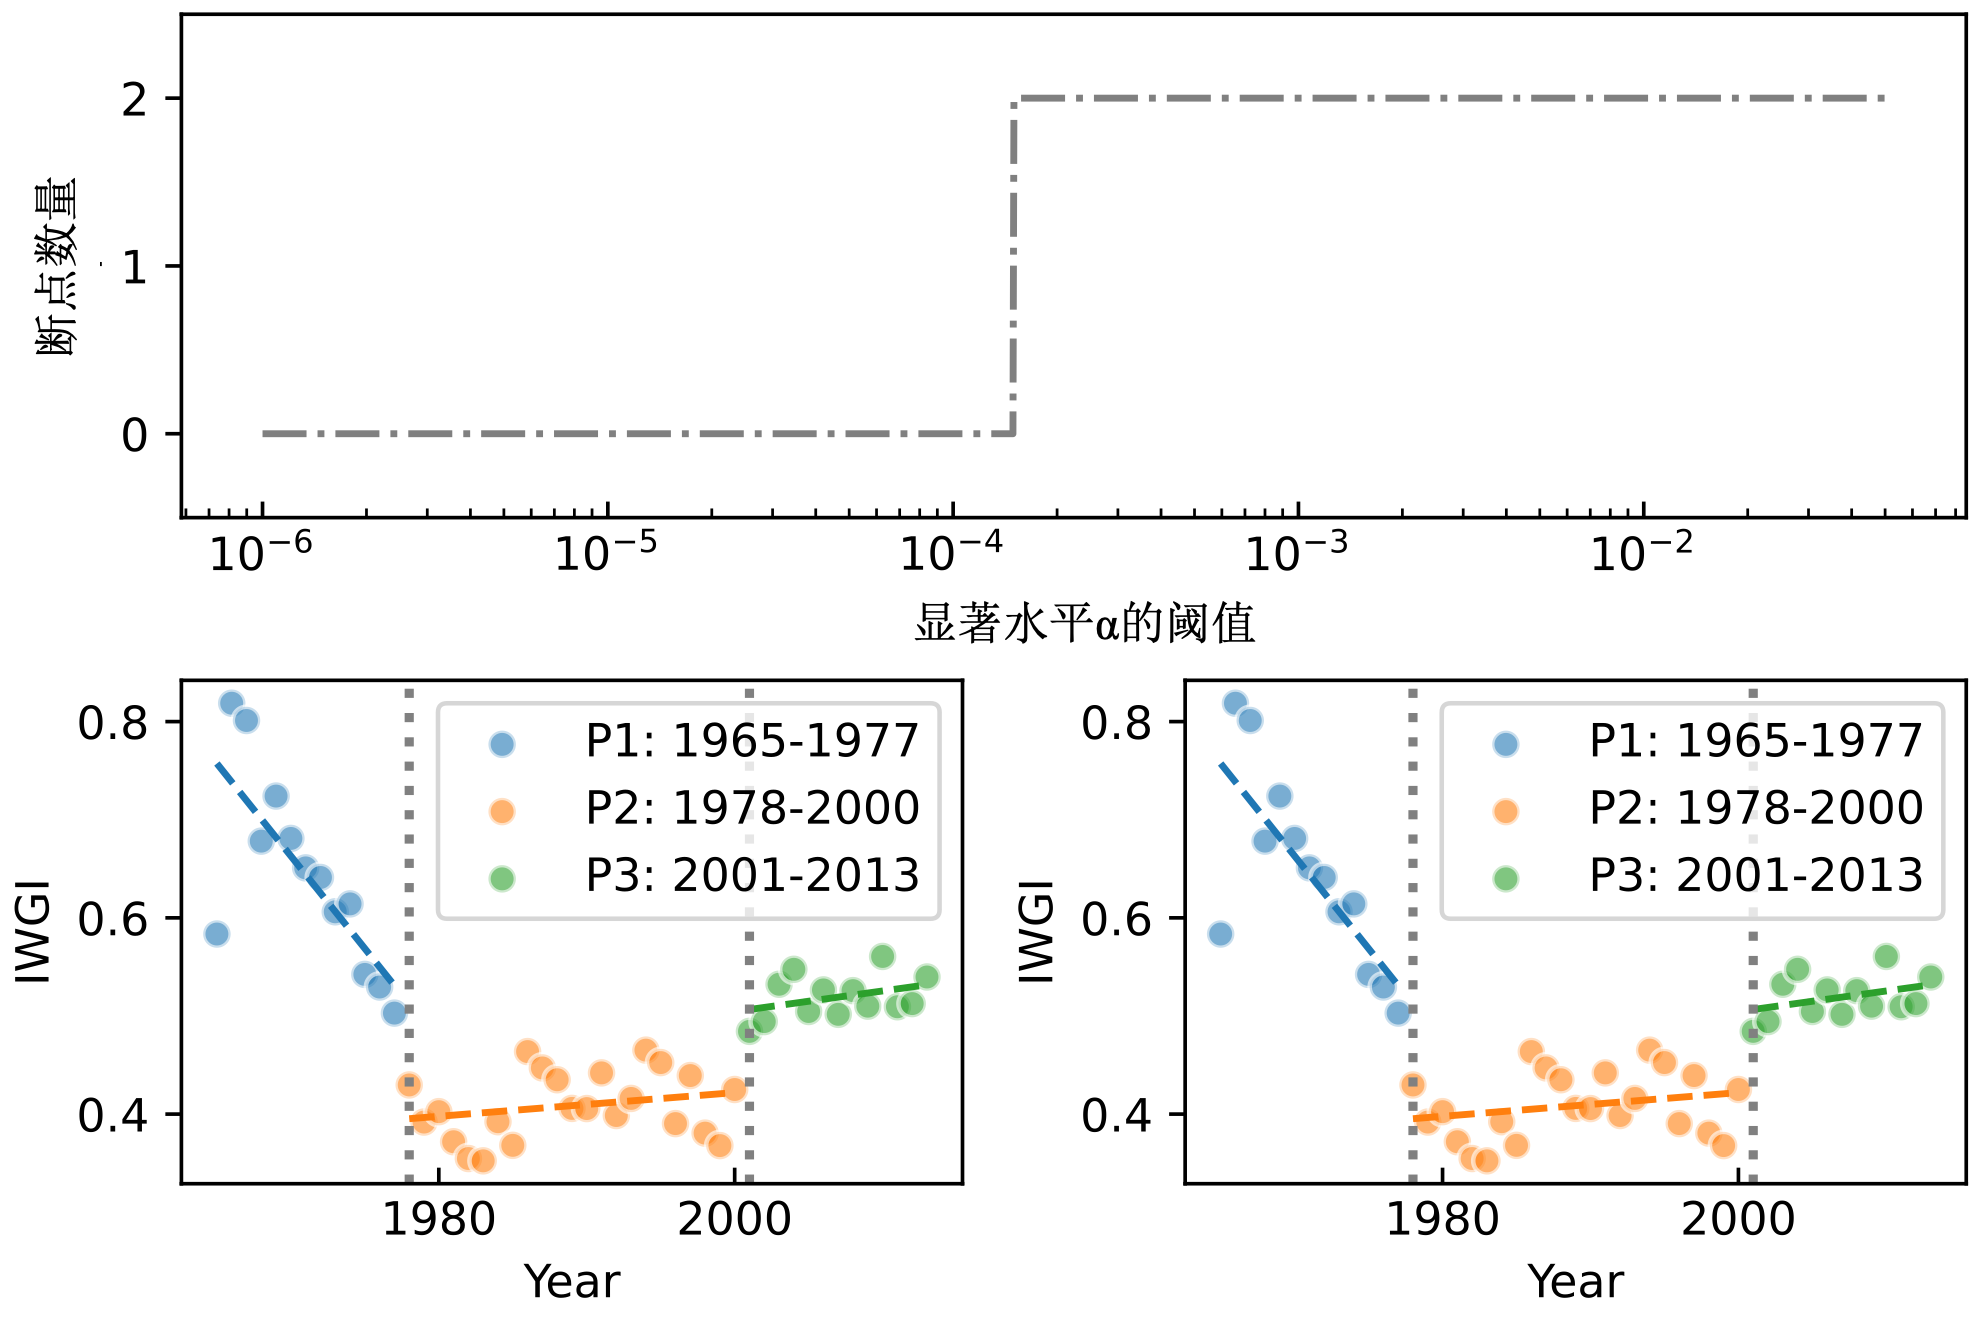
\includegraphics[width=\textwidth]{img/ch4/ch4_sensitivity.png}
    \caption[突变点检测中显著性阈值选取的敏感性测试]{突变点检测中显著性阈值选取的敏感性测试结果。
    \textbf{A} 选取不同阈值$\alpha$后识别的突变点个数,所有的方案都识别了两个断点。
    \textbf{B} 阈值选取为 $\alpha=0.0005$.
    \textbf{C} 阈值选取为 $\alpha=0.05$.}\label{ch4:fig:sensitivity}
\end{figure}

\subsection{数据来源}

% % Table generated by Excel2LaTeX from sheet '数据集'
\begin{table}[htbp]
    \centering
    \caption{数据分类与来源}
      \begin{tabularx}{\textwidth}{LLLLL}
      \toprule
      数据集   & 数据类型  & 空间尺度  & 时间尺度  & 数据来源 \\
      \midrule
      行政区水资源利用 & 统计    & 市级行政单元 & $1965-2013$ & Zhou等人2020 \\
      子流域水资源使用 & 统计    & 二级子流域 & $2003-2019$ & 水资源公报 \\
      GDP数据 & 统计    & 省级行政单元 & $1949-2019$ & 万德数据库 \\
      水库数据集 & 水文    & 站点数据  & $1949-2015$ & Wang等人2019 \\
      实测泾流量 & 水文    & 站点数据  & $1949-2019$ & Wang等人2019 \\
      黄河流域相关法律 & 文献    & 流域相关文件 & $1949-2013$ & 黄河流域规划 \\
      黄河水利委员会历史 & 文献    & 流域相关文件 & $1949-2002$ & 黄河水利委员会档案馆 \\
      黄河大事件 & 文献    & 流域相关文件 & $1949-2015$ & 黄河水利委员会档案馆 \\
      \bottomrule
      \end{tabularx}%
    \label{ch4:tab:data_source}%
\end{table}%
  

为了计算IWGI,使用了三个数据集:水库、实测径流、和用水。
水库数据集由Wang等人~\cite{wang2019c}收集,其中包括1956年以来新建的重要水库。
在所有水库中,黄河水利委员会已经将主要用于调节和管理的水库称为``主要水库''(见\url{http://www.yrcc.gov.cn/hhyl/sngc/})。
此外,每年的实测径流数据来自《黄河泥沙公报》(\url{http://www.yrcc.gov.cn/nishagonggao/}),分别由四个控制站(唐乃亥、头道拐、花园口、利津)在黄河的不同河段(源区、上游、中游、下游)进行测量得到。
水资源利用数据来源于Zhou等人\cite{zhou2020}发布的中国国家长期水资源利用数据集(NLWUD),包括地级市不同部门的用水量、用水经济变量和用水强度,我们以$95\%$相交面积为阈值筛选该数据集中的地级市,得到属于黄河流域的子数据集。

为了分析其变化的原因,灌溉面积、工业增加值和服务业总增加值以及用水强度数据也来自NLWUD数据集~\cite{zhou2020}。
此外,还使用了两个水治理政策数据集:法律政策和``大事件''文件数据集。
法律政策记录(表~\ref{ch4:tab:policies})来源于2013年公开批准的``黄河流域综合规划'',其中回顾了建国以来全流域尺度上的重要法律法规。
与黄河有关的``大事件''的原始文件则来自黄河水利委员会的记录和汇编(\url{http://www.yrcc.gov.cn/hhyl/hhjs/})。

本研究中使用或分析的所有数据,包括水库数据集、测量径流、用水数据集、规律和大事件,都已储存在公开获取的数据仓库中(\url{https://doi.org/10.5281/zenodo.7955500}~\cite{shuang_song_2023_7955500})。

% Table generated by Excel2LaTeX from sheet '黄河流域法律政策'
\begin{table}[htbp]
    \centering
    \caption{黄河流域法律政策}
      \begin{tabularx}{\textwidth}{L p{1.5cm} L}
      \toprule
      法律或政策名称 & \multicolumn{1}{l}{施行或修订时间} & 颁布机构 \\
      \midrule
      中华人民共和国水法 & 1,988 & 全国人民代表大会常务委员会 \\
      中华人民共和国水法  修正 & 2,002 & 全国人民代表大会常务委员会 \\
      中华人民共和国水法  第一次修订 & 2,009 & 全国人民代表大会常务委员会 \\
      中华人民共和国水法  第二次修订 & 2,016 & 全国人民代表大会常务委员会 \\
      中华人民共和国水污染防治法 & 1,984 & 全国人民代表大会常务委员会 \\
      中华人民共和国水污染防治法  修正 & 1,996 & 全国人民代表大会常务委员会 \\
      中华人民共和国水污染防治法  第一次修订 & 2,008 & 全国人民代表大会常务委员会 \\
      中华人民共和国水污染防治法  第二次修订 & 2,018 & 全国人民代表大会常务委员会 \\
      取水许可和水资源费征收管理条例 & 2,006 & 中华人民共和国国务院 \\
      取水许可和水资源费征收管理条例  第一次修订 & 2,017 & 中华人民共和国国务院 \\
      黄河水量调度条例 & 2,006 & 中华人民共和国国务院 \\
      黄河可供水量分配方案 & 1,987 & 中华人民共和国国务院 \\
      取水许可管理办法 & 2,008 & 中华人民共和国水利部 \\
      取水许可管理办法  第一次修订 & 2,015 & 中华人民共和国水利部 \\
      取水许可管理办法  第二次修订 & 2,017 & 中华人民共和国水利部 \\
      黄河水量调度条例 & 2,006 & 中华人民共和国国务院 \\
      黄河可供水量年度分配及干流水量调度方案 & 1,998 & 国家发展计划委员会,水利部 \\
      黄河水量调度管理办法 & 1,998 & 国家发展计划委员会,水利部 \\
      黄河水权转换管理实施办法 & 2,004 & 水利部 \\
      取水许可和水资源费征收管理条例 & 2,006 & 中华人民共和国国务院 \\
      取水许可证制度实施办法 & 1,993 & 中华人民共和国国务院 \\
      建设项目水资源论证管理办法 & 2,002 & 国家发展计划委员会,水利部 \\
      水利工程管理体制改革实施意见 & 2,006 & 中华人民共和国国务院 \\
      \bottomrule
      \end{tabularx}%
    \label{ch4:tab:policies}%
  \end{table}%
  

\subsection{数据分析}

\subsubsection{相关分析与显著性检验}

皮尔逊相关系数(Pearson correlation coefficient,通常用 $r$ 表示)是用于衡量两个连续变量之间线性关系强度的指标。它的值范围在 $-1$ 到 $1$ 之间,其中 $-1$ 表示完全负相关,$1$ 表示完全正相关,$0$ 表示无相关性,本研究使用该指标反映某时段内IWGI的趋势同哪些子指标变化趋势更密切,为了计算两个变量之间的皮尔逊相关系数,我们可以使用以下公式\cite{freedman2007}:

\begin{equation}
    r = \frac{\sum_{i=1}^{n}(x_i - \bar{x})(y_i - \bar{y})}{\sqrt{\sum_{i=1}^{n}{(x_i - \bar{x})}^2}\sqrt{\sum_{i=1}^{n}{(y_i - \bar{y})}^2}}
\end{equation}

其中,$x_i$ 和 $y_i$ 分别表示第 $i$ 个观察值,$\bar{x}$ 和 $\bar{y}$ 分别表示 $x$ 和 $y$ 的均值,$n$ 表示观察值的数量。计算出皮尔逊相关系数后,我们需要进行显著性检验来确定这种关系是否具有统计显著性。这里我们使用 $t$ 检验来计算显著性水平。根据 $r$ 和样本大小,我们可以计算 $t$ 值\cite{freedman2007}:

\begin{equation}
    t = \frac{r\sqrt{n-2}}{\sqrt{1-r^2}}
\end{equation}

根据统计量$t$的值查表判断显著性水平,如果 $p$ 值低于预先设定的显著性水平$0.01$,则我们可以认为两个变量之间的关系具有统计显著性。在实际应用中,我们使用 scipy 1.10.1~\cite{2020SciPy-NMeth}完成这些计算。

\subsubsection{基于平均的指标贡献度}

本研究中,表征稀缺情况的SFV指数就是稀缺性(S)、弹性(F)、易变性(V)三个指标在不同区域(源区、上游、中游、下游)之间的等权重平均(见式\ref{ch4:eq:scarcity}),综合水治理指标(IWGI)则是稀缺情况、使用目的、分配方式三个子指标取对数后的等权重平均(见式\ref{ch4:eq:IWGI})。
对此类指数,本研究中使用如下方法计算某时段某子指标($X$)对总指标变化(或指标/地区均值)的贡献度$Contribution_{X}$:

\begin{equation}
    Contribution_{X} = \Delta_{X} / \Delta_{Index}
\end{equation}

其中$\Delta_{X}$是该子指标在给定时段(从$t=start$到$t=end$)内的总变化值,$\Delta_{I}$是该子指标参与贡献的总指标总变化,两者都可以使用如下公式计算:

\begin{equation}
    \Delta=\sum_{t=start}^{end}(X_{t}-X_{t-1})
\end{equation}

上述计算方法可以计算不同时间段、不同指标的贡献度,帮助了解各指标在特定时间段内对总体变化的影响程度。

\subsubsection{基于比例的指标贡献度}

本研究中供给性用水比例(表征使用目的,见式\ref{ch4:eq:priority})以除法形式进行计算,在分解各部门用水对比例变化的贡献时应取对数:

\begin{equation}
    \log{(\text{ratio})}=\log{\frac{A}{B}} = \log{A} - \log{B}
    \label{ch4:eq:log}
\end{equation}

本章感兴趣的是在时段开始($start$)到结束($end$)之间 $C$、$A$ 和 $B$ 的变化,我们可以将 C 的变化量表示为 A 和 B 变化量的加权和:

\begin{equation}
    \begin{aligned}
    & \Delta \log (C)=\log \left(C_{end}\right)-\log \left(C_{start}\right) \\
    & \Delta \log (A)=\log \left(A_{end}\right)-\log \left(A_{start}\right) \\
    & \Delta \log (B)=\log \left(B_{end}\right)-\log \left(B_{start}\right) \\
    & \Delta \log (C)=k_1 \cdot \Delta \log (A)+k_2 \cdot \Delta \log (B)
    \end{aligned}
\end{equation}

结合式\ref{ch4:eq:log},可以得到A 和 B 分别对 C 变化的贡献比例 $k_1$ 和 $k_2$:

\begin{equation}
    \begin{gathered}
    k_1=\frac{\Delta \log (C)}{\Delta \log (A)} \\
    k_2=\frac{\Delta \log (C)-\Delta \log (A)}{-\Delta \log (B)}
    \end{gathered}
\end{equation}


\section{人类活动主导时期人水关系演变过程}\label{ch4:process}
\subsection{综合指标变化过程}\label{ch4:sec:process}

\begin{figure*}[ht!]
	\centering
	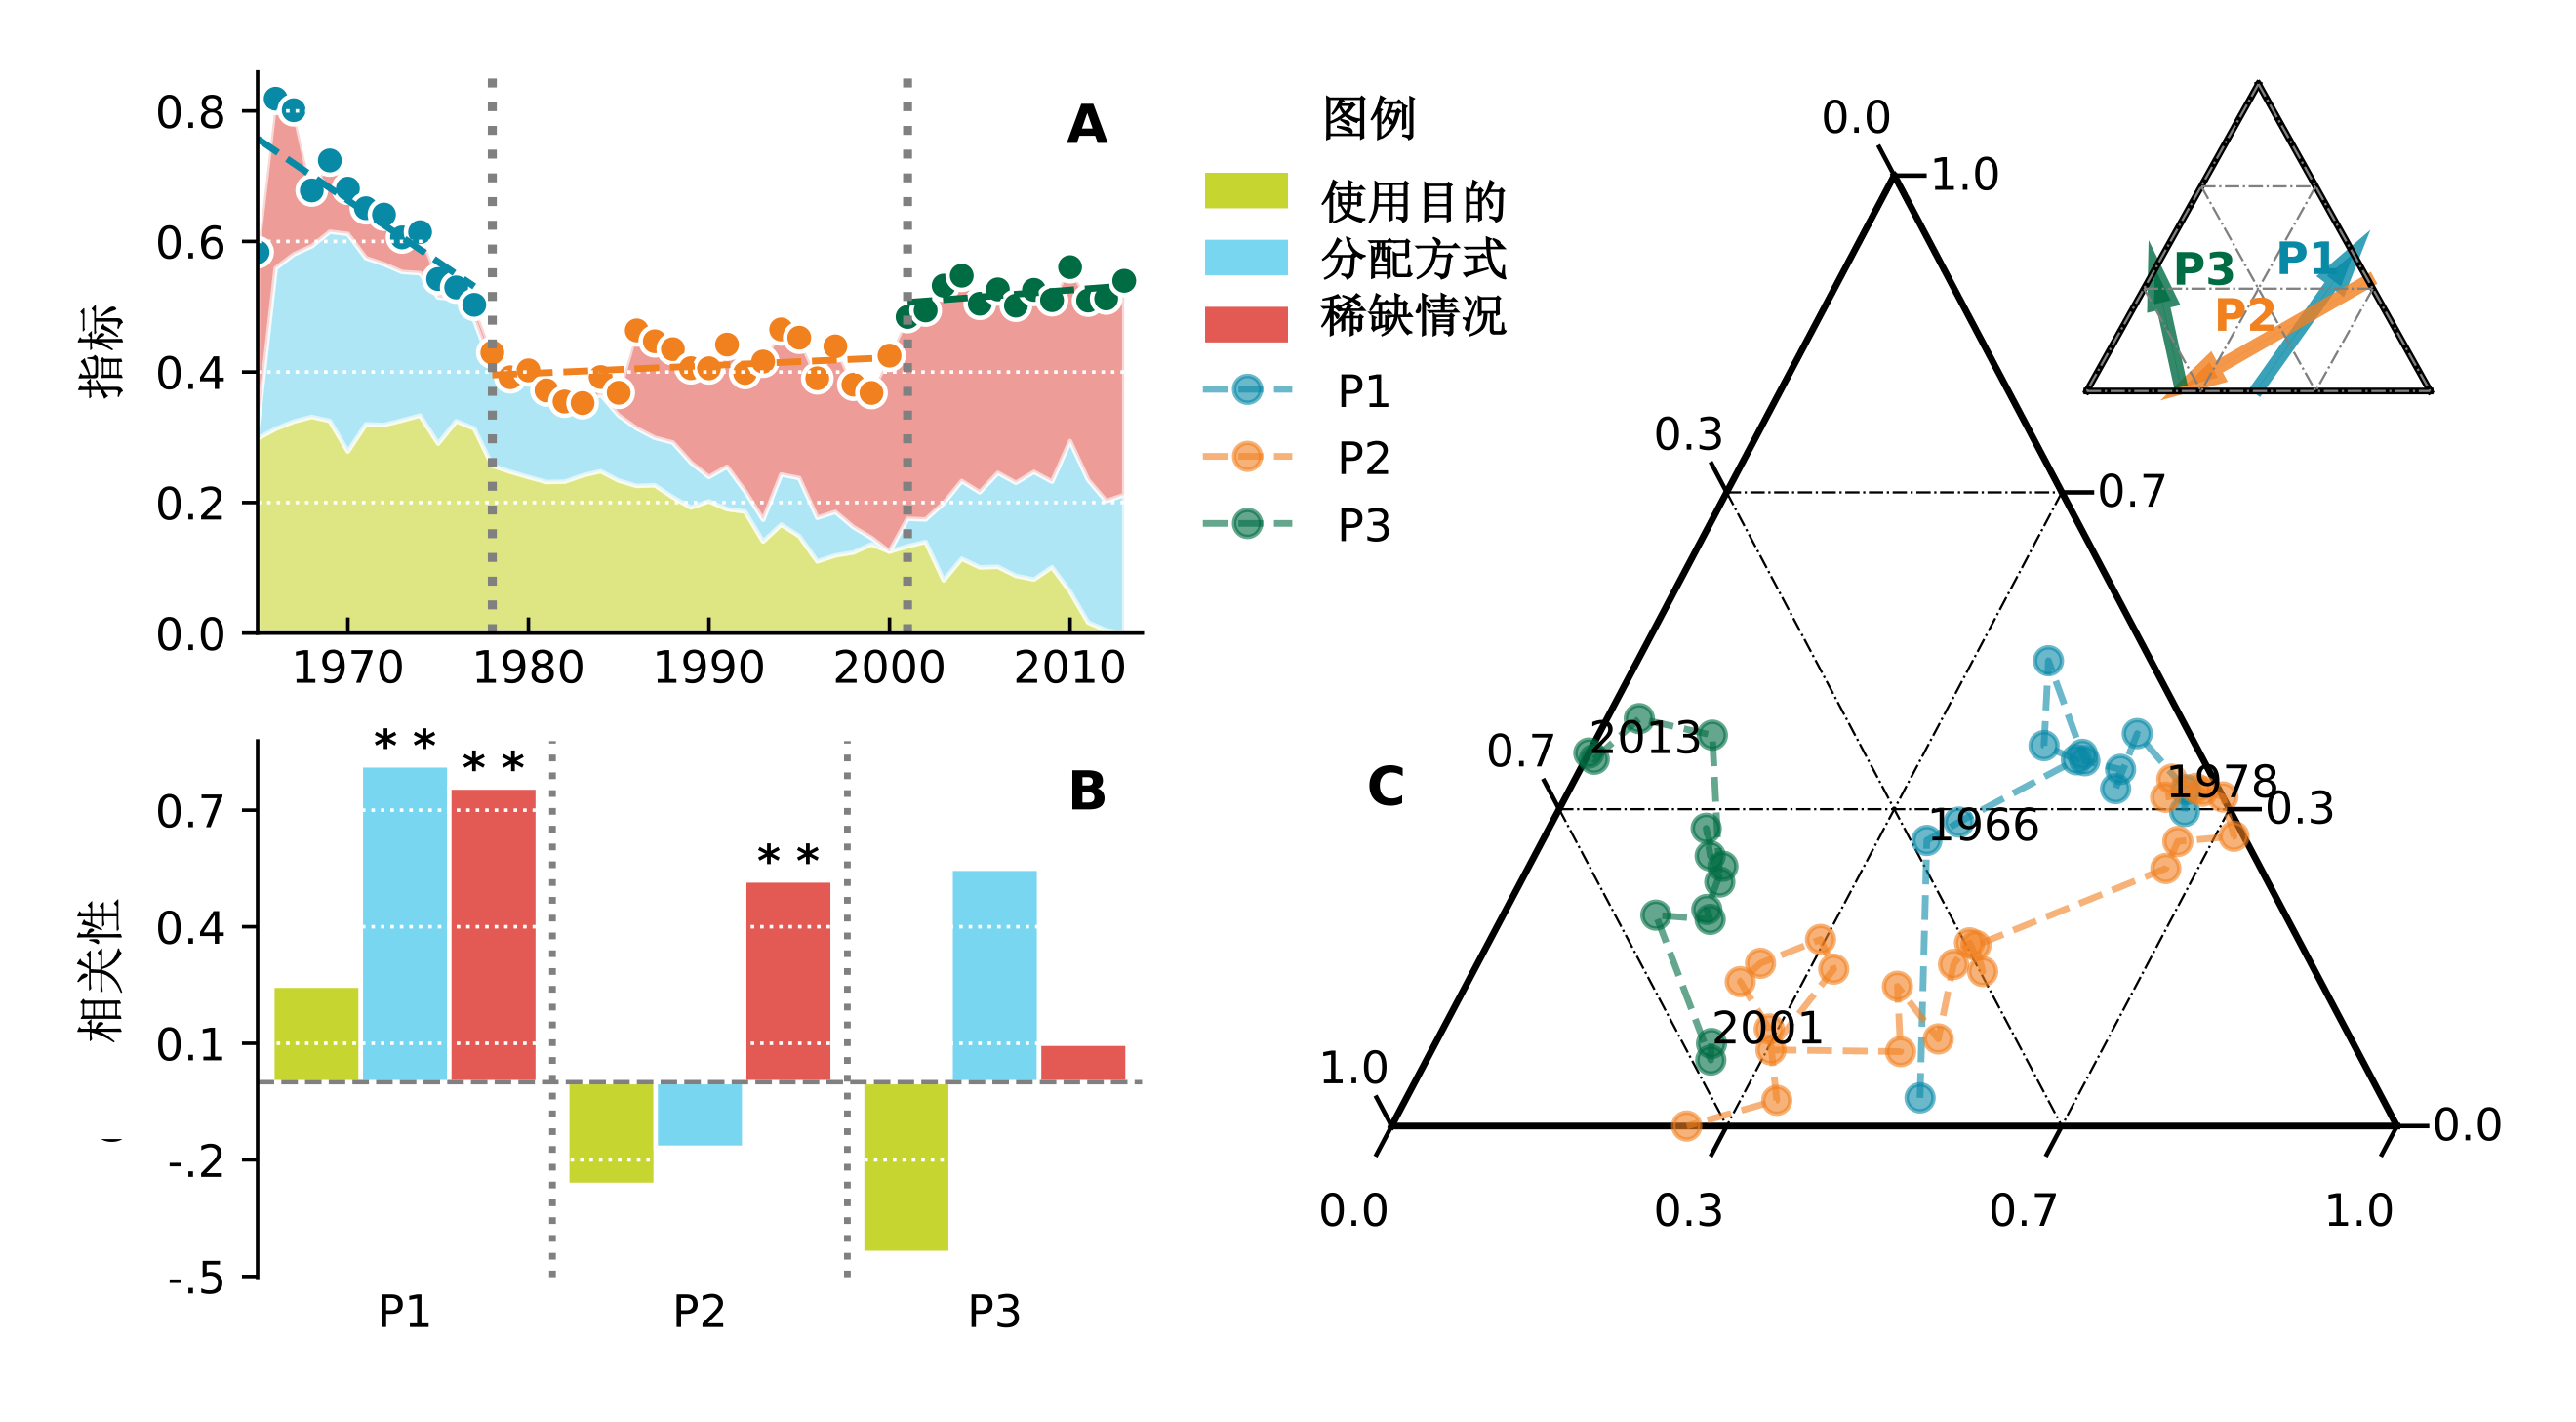
\includegraphics[width=\textwidth]{img/ch4/ch4_index.png}
	\caption[IWGI指数反映黄河流域的水治理变化阶段]{IWGI指数反映黄河流域的水治理变化阶段。两个突变点将1965年以来的黄河流域水治理划分为三个阶段,第一阶段(P1): $1965 \sim 1978$,第二阶段(P2): $1979 \sim 2001$,第三阶段(P3): $2002 \sim 2013$。
	\textbf{A,} 检测IWGI的突变点和三个指标的各自贡献:“稀缺情况(S)”、“使用目的(P)”和“分配方式(A)”。1978年和2001年出现了两个显著的变化点($p<0.01$)。
	\textbf{B,}  各阶段的IWGI变化与三个指标各自变化的相关性。
	\textbf{C,} IWGI随时间变化的同时,三个指标贡献比例的组合不断改变,致使水治理向不同方向发生阶段性转移。
	}\label{ch4:fig:IWGI}
\end{figure*}

IWGI在研究时段内存在两个突变点,将1965年以来的黄河流域水治理划分为三个阶段,第一阶段(P1): $1965 \sim 1978$,第二阶段(P2): $1979 \sim 2001$,第三阶段(P3): $2002 \sim 2013$,而“稀缺情况(S)”、“使用目的(P)”和“分配方式(A)”的三个指标在每个阶段的贡献不同(图~\ref{ch4:fig:IWGI}A)。
% 第一阶段
在第一个时期(P1, $1965 \sim 1978$)水资源压力对IWGI的贡献很小,“使用目的”和“分配方式”的指标的贡献更大(平均分别为$49.45\%$和$34.95\%$),但均呈现出显著的下降趋势($p<0.01$,图~\ref{ch4:fig:IWGI}~B),导致此时期IWGI迅速下降。
% 第二阶段
在第二阶段(P2, $1979 \sim 2001$),水资源压力指标的显著增加($p<0.01$)并为IWGI的略微上升做出主要贡献($p<0.01$,图~\ref{ch4:fig:IWGI}~A),而“使用目的”和“分配方式”的指标对IWGI的变化起了消极作用。
% 第三阶段
最后,在第三个时期(P3, $1995 \sim 2013$),尽管水资源压力指标在贡献中保持着$57.11\%$的最突出份额,但其数值已几乎保持不变,反而是“使用目的”的指标的降低和“分配方式”指标的增加,共同推动了综合指标IWGI的变化。
%的整体
综上所述,“稀缺情况(S)”、“使用目的(P)”和“分配方式(A)”的三个指标在不同时期对黄河流域水治理整体特征变化的贡献不同,将其演变历史划分为明显的三个阶段,依据其各自特点可命名为:集中供水时期、治理转变时期、适应增强时期(对应时间阶段分别为$1965 \sim 1978$、$1979 \sim 2001$、$2002 \sim 2013$(图~\ref{ch4:fig:IWGI}~C)。

\subsection{稀缺情况指标变化}

构成稀缺情况的指标(SFV指数)在研究时段(包括三个不同时期)内呈现出先降低、然后迅速增加、最后再次略微降低的变化趋势(图~\ref{ch4:fig:scarcity}~A)。
% ,表明水资源压力先减少再迅速增加,后趋于稳定
源区、上游、中游、下游这四个不同的区域中(图~\ref{ch4:fig:scarcity}~B),源区对三个时段的SFV指标变化几乎没有贡献,下游也仅在治理转变时期和适应增强时期呈现微弱的负向贡献。
对稀缺情况影响最大的是黄河的上游和中游,上游在集中供水时期和治理转变时期都是SFV变化的最大贡献区域,中游则在适应增强时期做出最大贡献。

\begin{figure}[!ht]
  \centering
  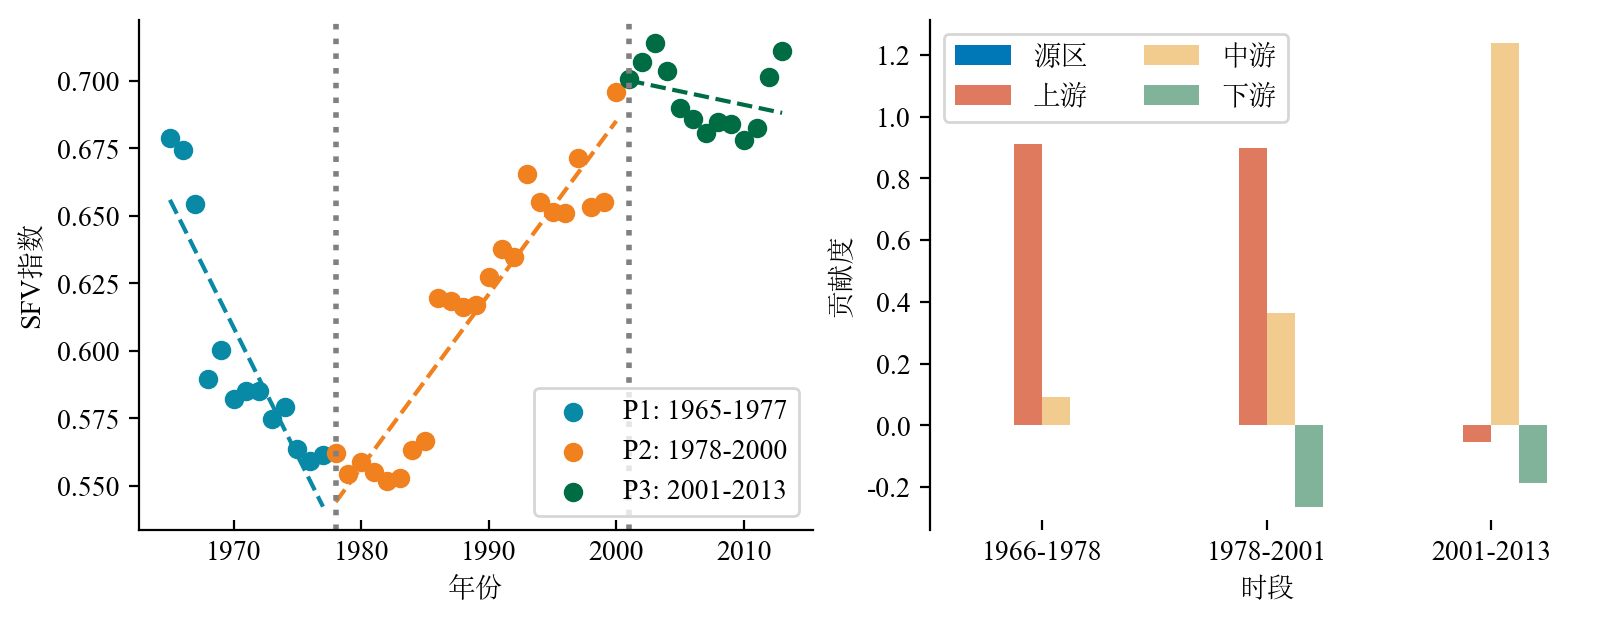
\includegraphics[width=\textwidth]{img/ch4/ch4_scarcity.png}
  \caption{稀缺性SFV指标变化趋势及各区域贡献}\label{ch4:fig:scarcity}
\end{figure}


\subsection{使用目的指标变化}

在用水目的上,供给性用水比例在集中供水时期基本保持不变,但在治理转变时期和适应增强时期呈现迅速下降的趋势(图\ref{ch4:fig:priority}~A)。
三个时段都是由灌溉用水的变化主导了该比例变化,城市、农村的人居用水、农村牲畜用水等几乎对该比例的变化没有影响(图\ref{ch4:fig:allocation}~B)。

\begin{figure}[!ht]
	\centering
	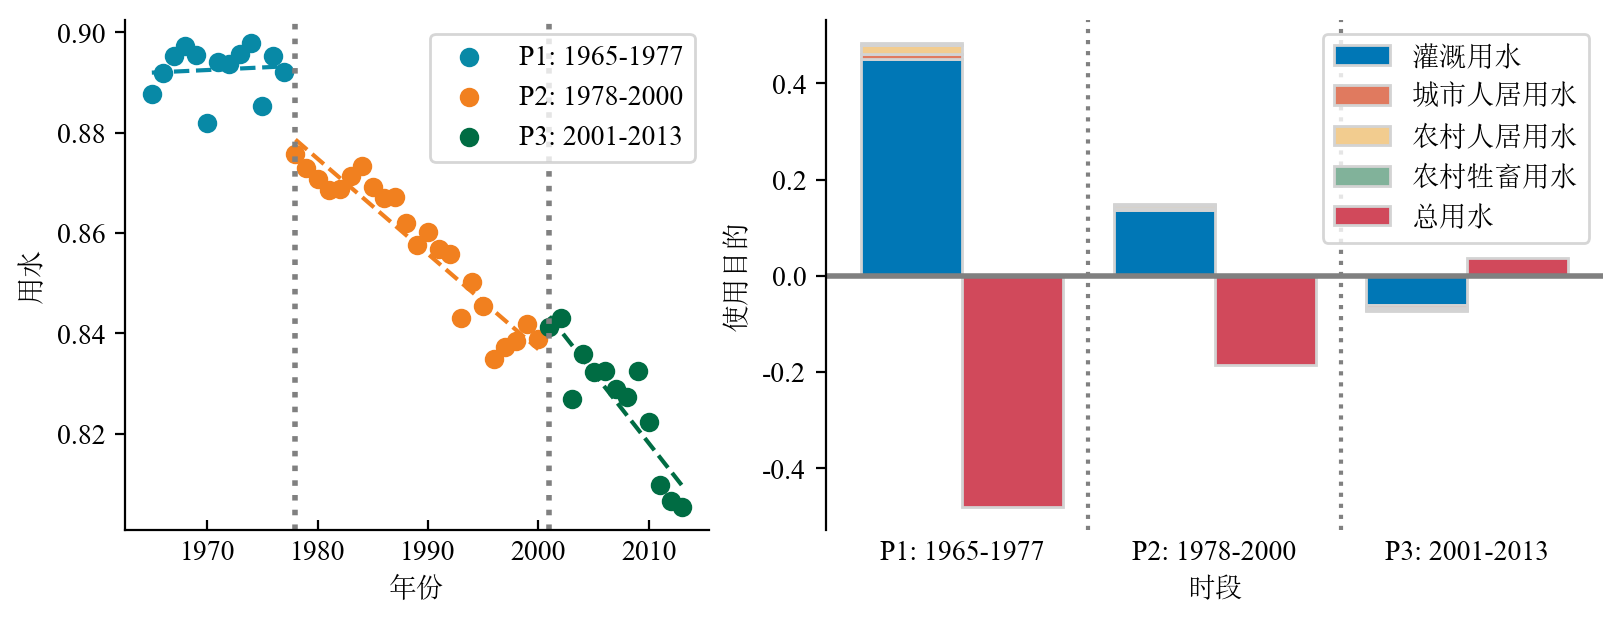
\includegraphics[width=\textwidth]{img/ch4/ch4_priority.png}
	\caption{供给性用水所占比例的变化趋势及各部门贡献}\label{ch4:fig:priority}
\end{figure}

\subsection{分配方式指标变化}

分配方式的指标变化呈现明显“V形”趋势,表明黄河的源区、上游、中游、下游之间水资源呈现先逐渐远离均匀分配,又在2000年后逐渐趋于平均的变化过程(图\ref{ch4:fig:allocation})。

\begin{figure}[!ht]
	\centering
	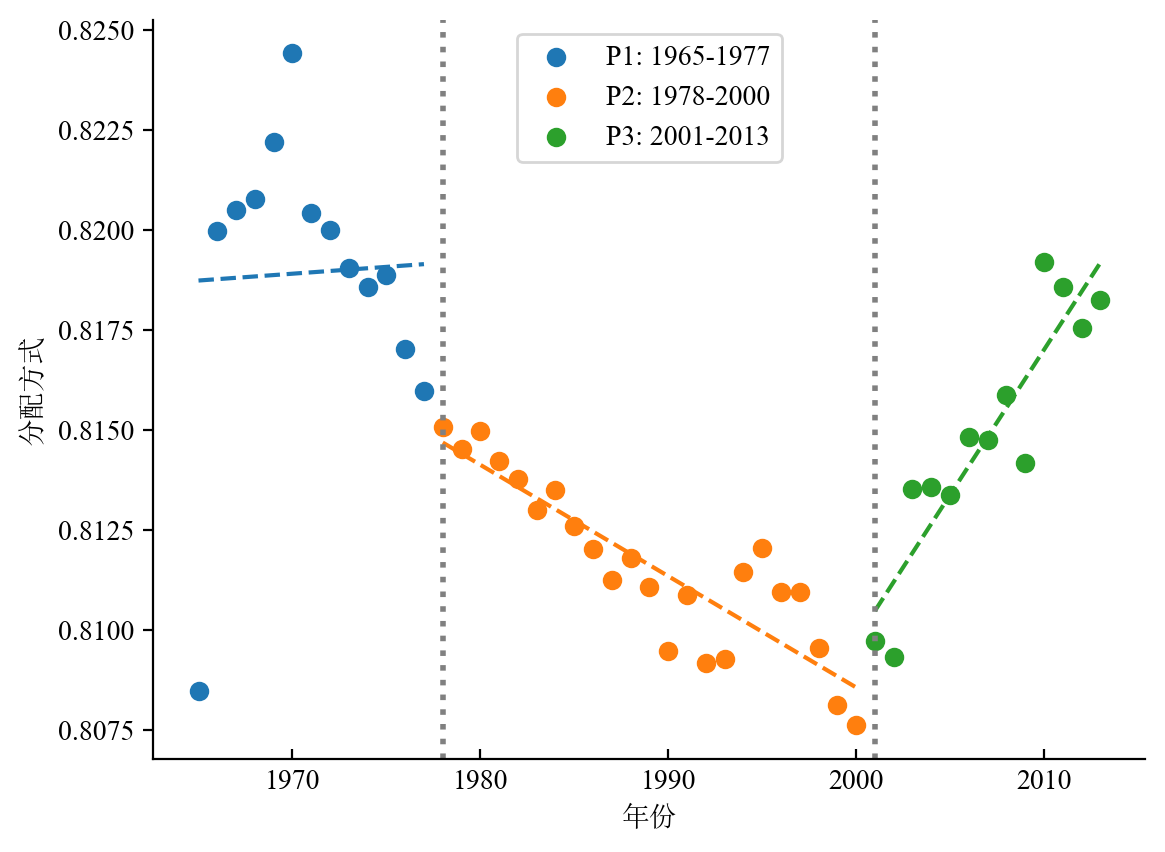
\includegraphics[width=0.6\textwidth]{img/ch4/ch4_allocation.png}
	\caption{分配方式指标的变化趋势}\label{ch4:fig:allocation}
\end{figure}

\section{人类活动主导时期人水关系演变机制}\label{ch4:mechanism}

% \subsection{水治理变化的驱动力分析}\label{ch4:sec:mechanism}

\begin{figure}[th!]
	\centering
	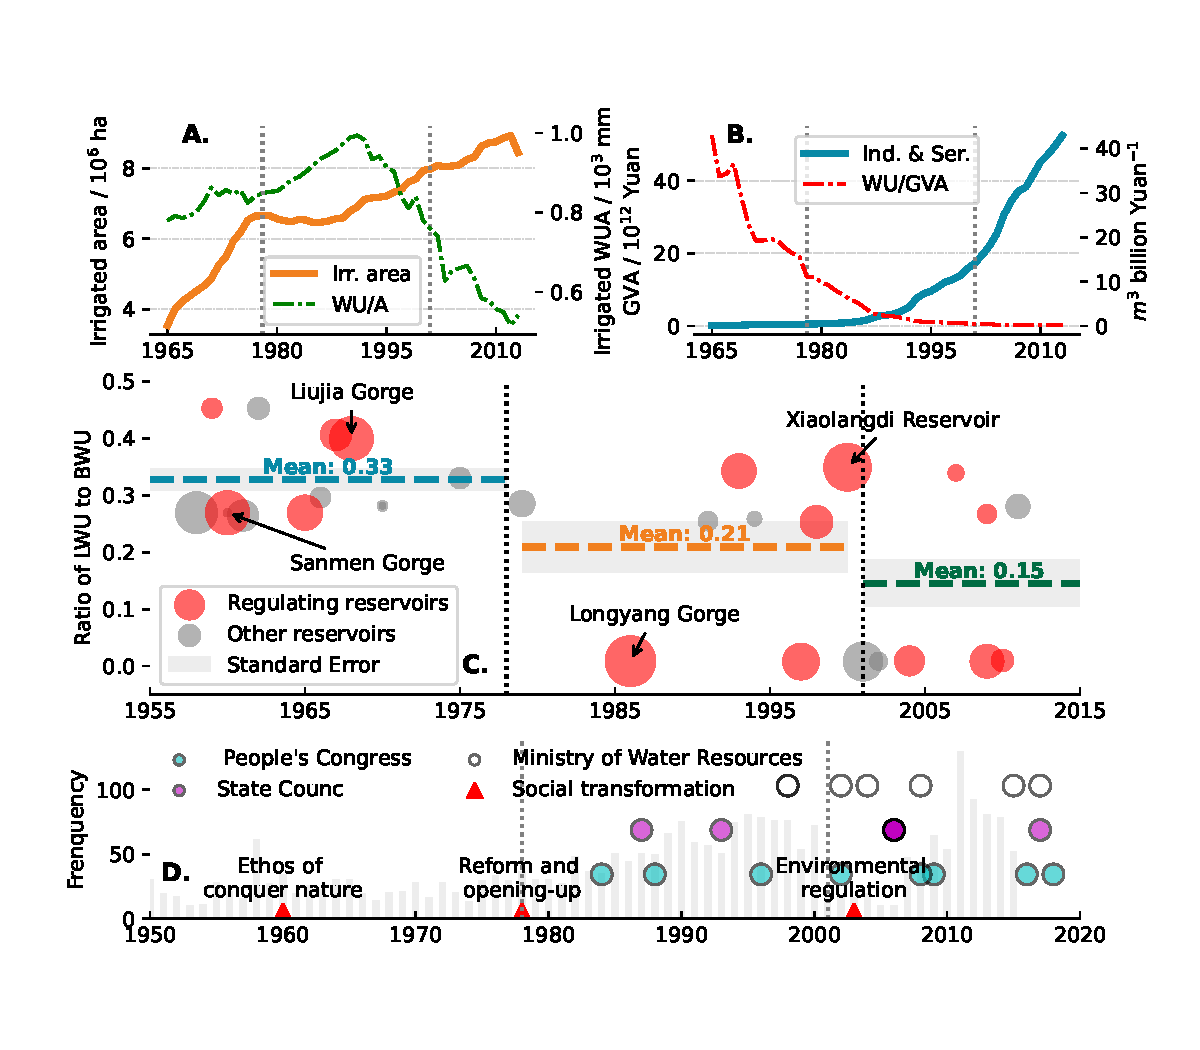
\includegraphics[width=\textwidth]{img/ch4/causes.pdf}
	\caption[黄河流域水治理阶段变化的驱动因素]{
		黄河流域水治理阶段变化的驱动因素。
		\textbf{A.}总灌溉面积($A$, 橙色线)和用水强度($WU/A$,用水量除以灌溉面积,绿点线)的变化。
        \textbf{B.}工业和服务业的总增加值(蓝线,$GVA$)变化及其用水强度($WU/GVA$,WU除以GVA,红点线)。
        \textbf{C.}每个水库的完工时间及其所在区域的用水量(Local Water Use, LWU)占水库完工时流域总用水量(Basinal Water Use, BWU)的百分比。红圈为负责黄河流域综合调度的水库。每个圆圈的大小表示其储水能力的大小。
        \textbf{D.}社会转型(红色三角形)和国家层面的治理政策(圆圈,不同颜色表示由不同的国家机构签署,越靠上代表国家机构的登记越高,详见表\ref{ch4:tab:policies})。浅灰色条形图以流域尺度(黄河大事件)计算与黄河流域有关的官方治理文献记录。}\label{ch4:fig:mechanism}
\end{figure}


\begin{figure}[tb]
    \centering
    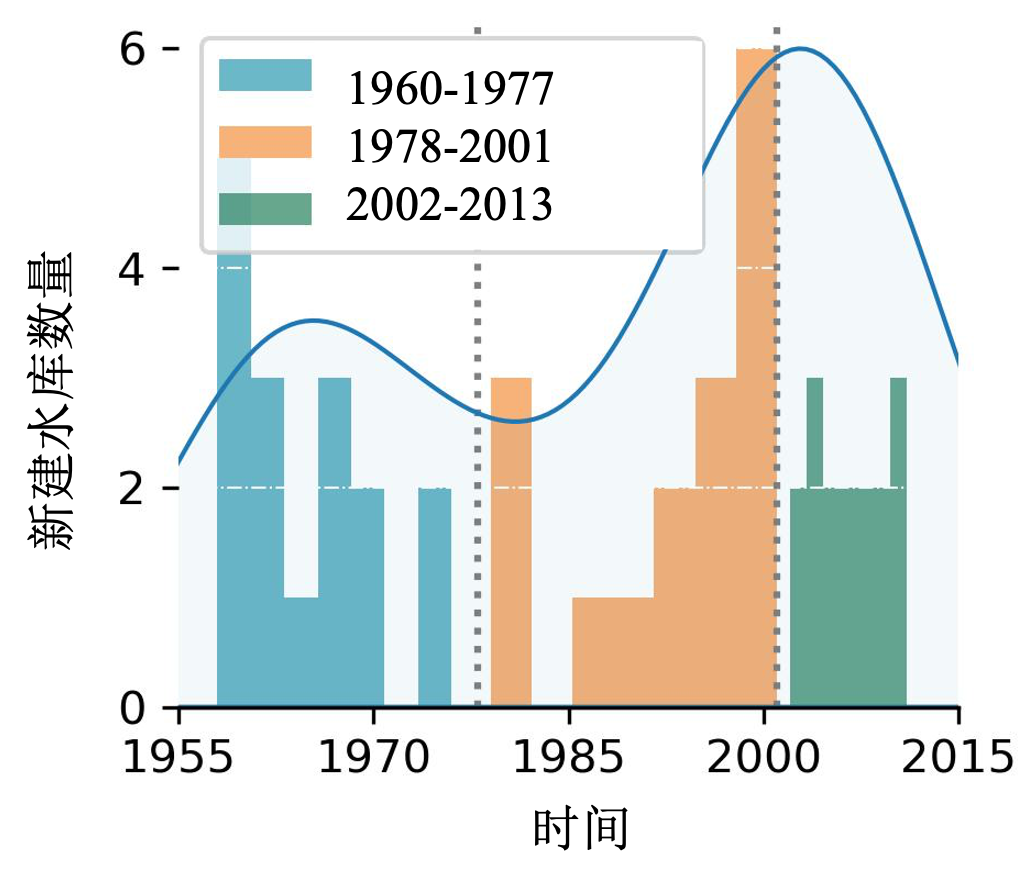
\includegraphics[width=0.6\linewidth]{img/ch4/ch4_reservoirs.png}
    \caption{黄河流域新增水库数量的时间分布}\label{ch4:fig:reservoirs}
\end{figure}


本节进一步探讨了致使IWGI变化的原因,灌溉区扩张和工业和服务业的经济增长是推动“集中供水时期”和“治理转变时期”两个阶段变化的关键。
黄河流域的用水需求在“集中供水时期”迅速增加,尤其是灌溉农业面积以$0.25*10^6 ha/yr$的速度迅速扩张(图\ref{ch4:fig:mechanism}~A),同时通过建设水库增加供应(图~\ref{ch4:fig:reservoirs})。
进入“治理转变时期”后,尽管灌溉区扩张停滞,但工业和服务业的发展开始增长,共同推动流域用水需求的进一步增加(图\ref{ch4:fig:mechanism}~A和B)。
接下来从“治理转变时期”到“适应增强时期”的演变过程中,水分利用效率变化最明显。
在“适应增强时期”,不仅工业和城市服务也承担了更重要的经济角色(由总增加值GVA表示,图\ref{ch4:fig:mechanism}~B),灌溉面积也恢复了缓慢扩张(图\ref{ch4:fig:mechanism}~A)。
但因用水效率的普遍提高,单位灌溉面积或单位产量的用水量都显著下降(图~\ref{ch4:fig:mechanism}~A和图~\ref{ch4:fig:mechanism}~B),因此部门和地区之间的用水差异在不断缩小,但流域水资源压力总体、持续维持在较高水平,公平合理分配宝贵水资源的压力越来越大(图~\ref{ch4:fig:IWGI}~A)。

最后,环境背景、社会文化、水治理政策等因素为三个时期的指标变化都产生了影响。
本研究首先计算了每个水库的区域用水量和流域用水量之比,较高的比值代表了该水库等潜在作用更有可能是旨在为该流域供水而不是流域调度;此外,流域调度的枢纽水库也以红色进行了标记(图~\ref{ch4:fig:mechanism}~C)。
可以看到,在阶段一的“集中供水时期”,受“人定胜天”的社会环境引领,大部分水库都建在需水量较大的地区,因此区域用水量和流域用水量之比值明显较高($p<0.01$,见图~\ref{ch4:fig:mechanism}~C)。
进入“治理转变时期”之后,新建水库的数量明显减少且多为枢纽水库,但全流域层次的法律法规(包括著名的“八七”分水方案)开始被不断提出,流域内的治理记录也迅速增加,可见此时期层出不穷的流域政策已深刻影响了流域水治理,流域水治理正在进行一场从工程措施向非工程措施的“治理转变”(图~\ref{ch4:fig:mechanism}~D, $p<0.01$和图\ref{ch4:fig:reservoirs})。
最后在“适应增强时期”,持续高位的水压力已成为制约区域发展的瓶颈,亟需通过节水转型和跨区域协调、调水来满足经济发展的用水需求,因此并且“大规模进行环境治理和节水转型”的国家战略指导下,有关部门提出了更多的、级别更高的水治理决策(图~\ref{ch4:fig:mechanism}~D)。
综上所述,从“集中供水时期”到“治理转变时期”的转变与当时水资源供需的增加相一致;而“治理转变时期”到“适应增强时期”的演变过程则是在水资源压力趋于稳定的同时,由社会监管政策和节水转型带来的效率提高所驱动的。

\section{讨论}\label{ch4:discussion}
\section{流域水治理演变模式}

研究结果显示黄河流域在人类主导时期有三种不同的流域治理模式:集中供水时期(P1: $1965 \sim 1978$)、治理转变时期(P2: $1979 \sim 2001$)和适应转向时期(P3: $2002 \sim 2013$)(图~\ref{ch4:fig:IWGI})。
在黄河流域水资源压力相对较低的集中供水时期($1965 \sim 1978$年),主要的水资源需求是为牲畜和作物等供给服务为目的,水治理也倾向于通过建造水库和引水渠等来增加水资源供给。
然而,正如当时“人定胜天”的口号所暗示的那样,水资源供应的增加并不能促进人-水关系和谐,因为它在不考虑生态保护的情况下急剧增加了用水,且这常常是一种不可逆转的变化\cite{zhou2020}。
在接下来的十年内,灌溉农田和引水设施的迅速扩张使黄河流域超负荷取水,在1972年以来,超过$80\%$的地表水被使用,导致河流频繁枯竭,造成了额外的生态问题,如湿地萎缩和生物多样性下降\cite{wang2019c}。
此外,由于水资源压力也限制了新兴的、更有利可图的工业与服务业的发展,这让流域的水治理模式接近了社会-生态危机的临界点,因为继续增加供应无论如何都是不切实际的\cite{loch2020, wohlfart2016a}。

治理体制转型时期的开始(P2: $1979 \sim 2001$)恰逢“改革开放”后,水资源竞争的持续加剧,但枯竭的黄河已经开始断流。
黄河流域在此时期开始水治理转变,这一结果与理论分析的结果高度一致:在流域总供应稳定的情况下,水资源需求在接近可供给水资源上限后的持续增长,将为流域水治理带来重大转型,流域社会-水文系统将通过制度措施让快速增强社会适应力,以响应该水资源供小于求的临界点\cite{loch2020}。
因此黄河流域在此时期发起了诸多水治理举措,包括控制灌溉面积的增长、倡导节水设施建设、制定全国首个水资源配额制度、并初步制定跨流域调水方案(南水北调)等\cite{wang2019b,long2020,nickum2021},成为了中国九大流域的制度变革先驱。
因此,尽管黄河流域的水资源压力仍然很大,且因径流减少和用水灵活性降低而持续增加,但黄河的断流问题却得到了解决,$1999$年的最后一次断流向世人昭示着此次水治理转变的巨大影响\cite{wang2019b}。

在随后的适应增强时期(P3: $2002 \sim 2013$)为适应稳定在高位的水资源压力,许多国家层面的黄河流域水治理实践都在这一时期提出,以期用最经济地方式,在保护生态的同时实现流域高质量发展。
二十一世纪初提出的“环境整治”和$2011$年提出的“最严格水资源管理”都是对水资源粗放式开发利用的响应,不断使流域水治理模式变得更高效。
这一时期除了中央政府主导的适应举措,地区各部门之间为了追求生产效率,社会经济过程为“水怎么用、水怎么分”的权衡发挥了重要作用。
典型的例子是黄河流域的水权转换工作,许多地区都积极推动了农业节水转型,并将节约的水额供给到经济效益更高的工业服务业之中。
通过不同行业和地区对流域水资源的广泛重建,通过日益强化的社会-经济过程调整以前粗放的发展模式以及刚性的制度约束,这些都是水治理适应性增强的体现,才能在有限的供水条件下优化平衡来自不同地区、不同行业的需求\cite{dalin2015,song2022}

黄河流域的水治理演化过程是“增大供给、治理转变、适应增强”的突出的案例,而其中变化的内在机制已在世界人类主导流域社会-水循环的过程中广泛出现(图~\ref{fig:summary})。
随着社会-经济过程对水循环影响加深,不同时期的流域面临不同的水治理挑战:在前期主要是经济和环境方面,在后期集中于与制度和政策方面。
放眼全球其它流域,以水资源短缺和供水困难为代表的水治理挑战是制约发展中流域的瓶颈\cite{allan2019,speed2013,liu2012a}。
人类社会-经济过程主导的发达流域(特别是跨界河流)则须重点解决结构性挑战,如水纠纷或缺乏公平\cite{mirumachi2015}。
本章研究开发并使用的综合水治理指数(IWGI)可以将流域水治理变化过程与这些挑战联系起来,提供了一种解释人类活动主导下人-水关系变化的方法。

\begin{figure}[htbp!]
	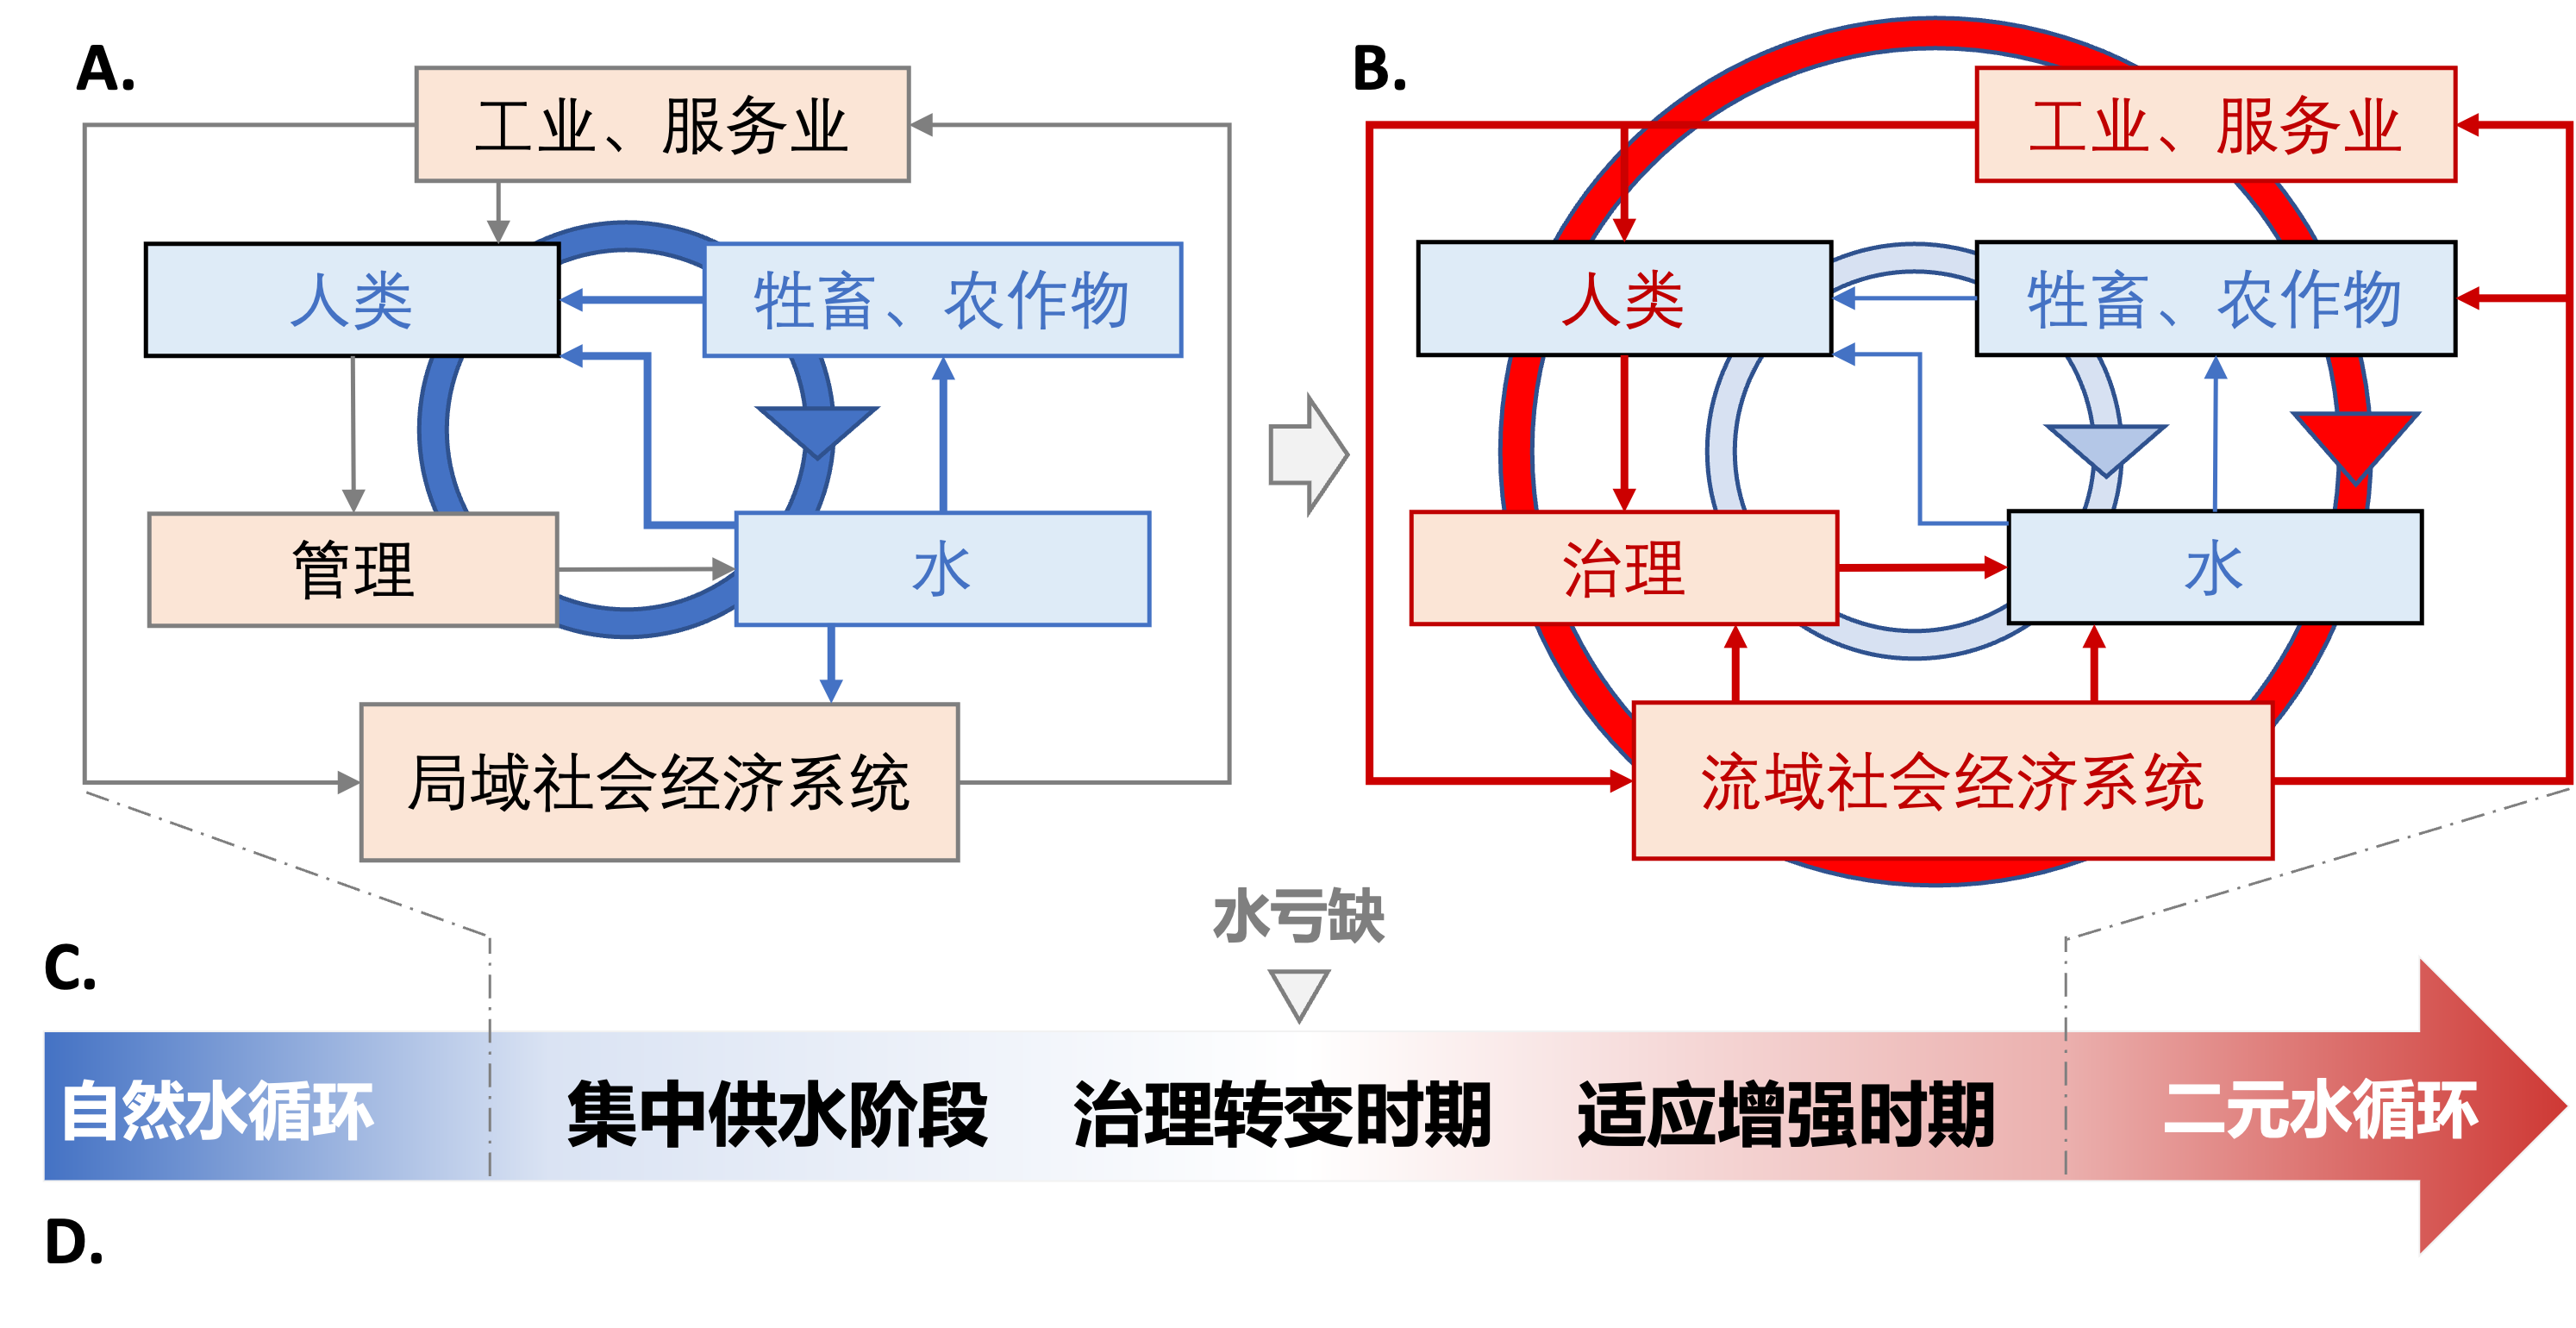
\includegraphics[width=\textwidth]{img/ch4/ch4_transition.png}
	\caption[人类主导下流域系统的水治理阶段过渡]{
		人类主导下流域系统的水治理变化过程。蓝色代表人类活动尚未成为主导的社会-水文循环,红色代表由社会经济过程主导的流域水过程。
        \textbf{A.}随着社会经济系统的发展,用以非供给服务的水需求增加;同时,通过水库等工程措施使人们能够控制水循环并局部缓解水资源压力。
        \textbf{B.}随着人为干预升级,不同地区和部门间的用水权衡愈发突出;流域亟需提升利用效率和调度能力,并组织起的更具适应性的水治理。
        \textbf{C.}在人类主导的流域社会-水文循环模式下,水治理转变常发生在水资源亏缺之后,在社会-经济过程主导下推动适应能力快速增长。在此之前水治理主要面临经济和环境挑战,但随后面临社会和政策挑战。
	}\label{fig:summary}
\end{figure}

\section{对流域治理规律的启示}

通过在数据丰富的黄河流域进行应用,本章研究表明所有的水治理问题都会导致“谁获得水、何时获得水以及如何获得水”的改变,因此监测“有多少水、怎么用、怎么分”三个关键问题对识别流域水治理变化有极大帮助。
但在世界范围内广泛应用该方法的主要局限是缺乏全球尺度的长时间序列数据,这意味着IWGI的可能缺点是难以推广。
在数据相对不足的流域应用IWGI时,建议不同方面的指标选择可根据现有数据集进行调整,因为底层指标之间关系的变化趋势比精确计算指标更重要。
在当今这个“人类世”,人-水关系由人类活动所主导的情况越来越普遍,应对层出不穷的治理挑战已成为复杂的人-水系统的核心\cite{cumming2018,cumming2014,jaeger2019}。
许多流域仍在不断接近系统随时可能崩溃的“地球界限”\cite{gleeson2020, wang-erlandsson2022},只有更深入地理解流域水治理系统,结合非线性稳态变化和转型的思想,才能维持流域社会-生态系统的韧性并实现可持续、高质量发展\cite{falkenmark2019}。

% Implications
由于大型河流流域是生态系统服务、经济发展和人类福祉的关键来源,水治理逐渐从主要的地方问题成为国家或国际问题\cite{best2019,best2020}。
随着远程耦合在联系日益紧密的世界中提出了更多的水治理挑战,水治理的政权转变与不同的人与水的关系相一致\cite{diaz2019}。
这一过程反映了社会如何通过增强其在水社会循环中的适应能力来改变治理实践的建议,IWGI定量地确定了这一转变\cite{loch2020,turton1999}。
科学家和决策者认识到不断变化的治理挑战是至关重要的,因为在一个阶段下开发的模型、制度、工程和方法不一定适用于另一个治理阶段\cite{reyers2018}。


\section{小结}\label{ch4:summary}
% 本章整合了水文数据、统计数据、历史文献材料等多源数据,开发流域水治理综合指数(Integrated Water Governance Index, IWGI),利用突变点检测方法量化识别了二十世纪六十年代以来的黄河流域治理的阶段变化,并分析了转变发生的驱动因素。

本章研究表明,两个突变点可以将1965 - 2013 年的黄河流域水治理演变历史划分为明显的三个阶段,依据其各自特点可命名为:集中供水时期(1965 - 1978,P1)、治理转变时期(1979 - 2001,P2)、适应增强时期(2002 - 2013,P3),而“稀缺情况(S)”、“使用目的(P)”和“分配方式(A)”的三个方面的指标在各阶段为黄河流域水治理的特征变化做出了不同贡献。
进一步探讨致使IWGI变化的原因,灌溉区扩张及工业和服务业的经济增长是推动“集中供水时期”和“治理转变时期”两个阶段变化的主要原因,环境背景、社会文化等因素对不同阶段的指标变化都产生了影响,水治理政策是将“治理转变时期”推向“适应增强时期”的主要驱动力。

黄河流域的水治理演化过程是“增大供给、治理转变、适应增强”的突出的案例,而其变化规律已在全球由人类主导的流域社会-水文循环过程中广泛出现。
理解黄河流域水治理的变化规律,可以为快速变化的大河流域提供实现可持续性的重要理论依据。

% Implications
由于大型河流流域是生态系统服务、经济发展和人类福祉的关键来源,水治理逐渐从主要的地方问题成为国家或国际问题\cite{best2019,best2020}。
随着远程耦合在联系日益紧密的世界中提出了更多的水治理挑战,水治理的政权转变与不同的人与水的关系相一致\cite{diaz2019}。
这一过程反映了社会如何通过增强其在水社会循环中的适应能力来改变治理实践的建议,IWGI定量地确定了这一转变\cite{loch2020,turton1999}。
科学家和决策者认识到不断变化的治理挑战是至关重要的,因为在一个阶段下开发的模型、制度、工程和方法不一定适用于另一个治理阶段\cite{reyers2018}。
\label{chapter4}

	\chapter{黄河治理转型期的分水制度演变}\label{cha:5}
% 第四章研究表明,近百年来,人类活动对黄河流域社会-水文循环的主导,使得社会-经济的水资源需求超出了临界点,从而导致其水治理模式发生了深刻的转型。这个转型过程既包含了从下到上的利益相关者对有限水资源的开发、交易和利用,也包含了从上到下的中央决策者的制度变化。两者共同促使了当代黄河的人-水关系的演变。

% 本章专门研究了水资源分配制度这一典型的从上到下的制度变化,分析了它对黄河流域产生的影响。
% 通过政策、法律和规范等制度来重塑社会-生态系统结构,是导致流域人-水关系变化的重要原因之一,它影响了所有相关社会行动者、生态单元或社会和生态系统要素之间的相互作用\cite{lien2020, bodin2017b}。
% 有效的(或“匹配”的)制度能够在特定的时空和功能尺度上运作,平衡人类与生态系统之间的相互作用,支持社会-生态系统的可持续性\cite{epstein2015, wang2019c}。
% 已有证据表明,制度上的改良能够取得良好的水治理成果,如中国黑河流域的生态调水工程\cite{wang2019c},以及欧洲的协同水治理系统\cite{green2013})。
% 但社会-生态结构的匹配不是很普遍,因为在复杂的大河流域中,推动制度变化会建立或破坏很多社会主体和生态单元之间的关系,从而导致意想不到的长期影响。

本章通过$1980$至$2010$年间黄河流域的制度变迁设计了一个准自然实验,分析了自上而下的水资源分配制度变化如何重塑流域社会-生态系统结构,产生的不同治理效果以及对流域可持续性的影响。
本研究关注了1987年的``八七''分水方案和1998年的“流域统一调度”,通过抽象社会-生态系统构件的方法,从官方文件中勾勒出了制度前后的系统结构变化。
接下来,本章使用主成分分析法对影响区域用水量的经济增长、基础设施建设、和气候条件等特征进行降维;最后使用差分合成控制法(DSC)\cite{arkhangelsky2021}估算了没有发生制度转变的理论用水量,分析了系统结构变化和用水量间的因果联系。


\section{研究方法与数据来源}\label{ch5:methods}
%! Author = songshgeo
%! Date = 2022/3/10

为了更好地理解自上而下的制度变化对黄河流域产生的影响,本章以黄河流域的水资源分配制度为例,重点关注两次重大制度转变:1987年提出的``八七''分水方案和1987年的提出的流域统一调度。
研究选择水资源分配制度为切入点的主要理由如下:
(1)本章关注自上而下的制度变迁对人\textendash{}水关系的影响,而黄河的水资源配额制度是典型的由中央主导的改革,利益相关者(相关各省)之间没有相互作用。
(2)鲜有大型流域在同一制度上经历多次重大转变,1987和1987前后两次制度变革具有难得的可对比性,提供了绝妙的准自然实验。
(3)两次制度变化之间维持的时间周期足够长,便于对数据进行时间序列分析,且该研究时段完全覆盖了第三章中识别的“治理转变时期”。

本章研究重点关注上述两次水资源配额制度变化对1979年至2008年黄河流域的用水变化。
两次制度变迁将这段研究时期分为均匀的三个时间序列:1979\textendash{}1987年,1988 \textendash{}1998年,1999\textendash{}2008年。
本章首先详细介绍了两次制度变化的背景及特点,以及刻画其社会\textendash{}生态系统结构模式的方法。
接下来收集用以构建反事实推断模型的数据集并使用主成分分析(PCA)方法对其进行降维。
最后,利用差分合成控制法(DSC)构建了反事实推断模型\cite{arkhangelsky2021},估算了“如果没有发生制度转变”时的用水量,从而分析两种制度变迁对黄河流域各省份用水量变化的净影响。
% 最后,在理论讨论方面,本研究基于已确定的SES结构进行了边际效益分析,为观测到的用水变化模式提供了理论解释。

\subsection{制度背景介绍}\label{sec:yrb}

20世纪80年代,因大量地表水取用以及水库拦蓄等其他形式的人类干预(约占黄河地表径流量的$80\%$),黄河发生了连续的断流问题,造成严重的生态、经济和社会危机,包括湿地萎缩、作物缺水、和地区间水资源争夺~\cite{fu2021}。
为此,黄河流域率先实施了几项雄心勃勃的治理措施以缓解水资源压力,如水库联合调度、南水北调工程、以及本研究所关注的水资源配额制度\cite{long2020, wang2019b}。
上述措施共同使黄河已二十余年不再断流,被认为是一项重大的管理成就和世界河流恢复的奇迹。
虽然已有研究仔细评估了南水北调和水库建设等工程解决方案产生的影响\cite{long2020,wang2019c},但被认为对遏制断流问题贡献最大的水资源配额制度却缺乏评估\cite{wang2019b}。

水资源分配制度在全世界范围内都是普遍存在的流域管理制度,而黄河流域是我国首次实施此类制度的流域,其提出、实施、发展、改革等过程可概括如下\cite{wang2019b}:

\begin{itemize}
    % 1978年:因黄河断流,整理意见
    \item 1982年:水利部要求沿黄各省和黄河水利委员会制定黄河水资源规划\cite{wang2019, wang2019a}。
    \item 1983年:各省提出规划需求,首次拟定配额方案的额度。
    \item 1987年:分配额度调整并确定,分配计划正式实施。
    \item 1998年:流域统一调度改革实施。
    \item 2008年:各省制定新的水利规划,进一步细化水资源分配\cite{wang2019,wang2019a}
    % 详见\url{http://www.ccgp.gov.cn/cggg/zygg/gkzb/202107/t20210721_16591901.htm
    \item 2021年:对最早在1987年正式通过的水资源分配额度进行调整。
\end{itemize}

$2008$年的文件标志着该方案成熟并进入下一阶段,即黄河流域开始建立流域级、省级、地级市、区级的多级水配额制度,因此本章结合数据可获得性将研究范围选定在$1978$年至$2008$年,以两次制度变化的官方文件为基础进行结构分析。

% \href{http://www.gov.cn/zhengce/content/2011-03/30/content_3138.htm#}{http://www.mwr.gov.cn},最后访问:\today
1987年的官方文件传达了以下要点:

\begin{itemize}
	\item 该政策面向的目标是利益相关者(沿黄省或地区),流域尺度的黄河水利委员会没有在文件中被提及。
	\item 政策制定的首要考虑是解决断流问题。
	\item 各省被鼓励在此配额下制定自己的用水计划。
	\item 水资源供给无法满足需求对相关省(地区)是普遍现象。
\end{itemize}

% (\href{http://www.mwr.gov.cn/ztpd/2013ztbd/2013fxkh/fxkhswcbcs/cs/flfg/201304/t20130411_433489.html}{http://www.mwr.gov.cn}, last access: \today)
1998年“流域统一调度”的官方文件传达了以下要点:

\begin{itemize}
	\item 除了说明政策针对的各省区之外(\textbf{第一章第三条}),明确指出其用水需要黄河水利委员会进行申报,并由其组织和监管 (\textbf{第三章第十一条,第五章至第七章})。
	\item 优先考虑上、中、下游用水的总体规划(\textbf{第一章第一条})。
	\item 在与1987年政策相同的配额下,鼓励各省进一步将配额分配给下级行政部门(\textbf{第二章第六条、第八章第四十一条})。
	\item 强调“以水量决定需求”,各省用水理论上不能超过1987年分配的额度 (\textbf{第一章至第二章}).
\end{itemize}

\subsection{制度的结构模式}\label{sec:structures}

本章研究在对以上官方文件的基础上,对两次制度变迁后的流域水资源利用的社会\textendash{}生态结构模式按框架图\ref{fig:framework}进行了抽象。
在社会\textendash{}生态系统中广泛存在的结构模式,常被表示为社会要素与生态要素共同构成的局部网络,通过抽象系统中存在相互关系为节点和链接来刻画它们~\cite{bodin2017,kluger2020,guerrero2015}。
本研究参考 Wang 等人在黑河流域制度变化分析中对该方法的应用\cite{wang2019b},
从官方文件的叙述中将可供取水的河段作为生态单位、分水制度涉及的行政单元(黄河水利委员会)和利益相关者(沿黄各省)之间的关系概化为一般的结构模式(见图\ref{fig:framework})。
所有社会节点(省份和黄河水利委员会)与河段之间因水资源的取用或监管概化为生态连接,它们因黄河水资源相关的过程产生相互作用被概化为社会连接。
% 19``八七''分水方案要求黄河水利委员会监测每条河流的范围,而19流域统一调度要求黄河水利委员会和各省之间直接互动(通过用水许可证)。
% 因此,本研究将黄河水利委员会单元与``八七''分水方案之后的每个生态单元和流域统一调度之后的每个省份单元联系起来。
% 本研究测试了关注社会经济体系结构而非制度细节是否能够合理解释黄河流域中由制度转变引起的差异。

\begin{figure}[!ht] % use float package if you want it here
    \centering
    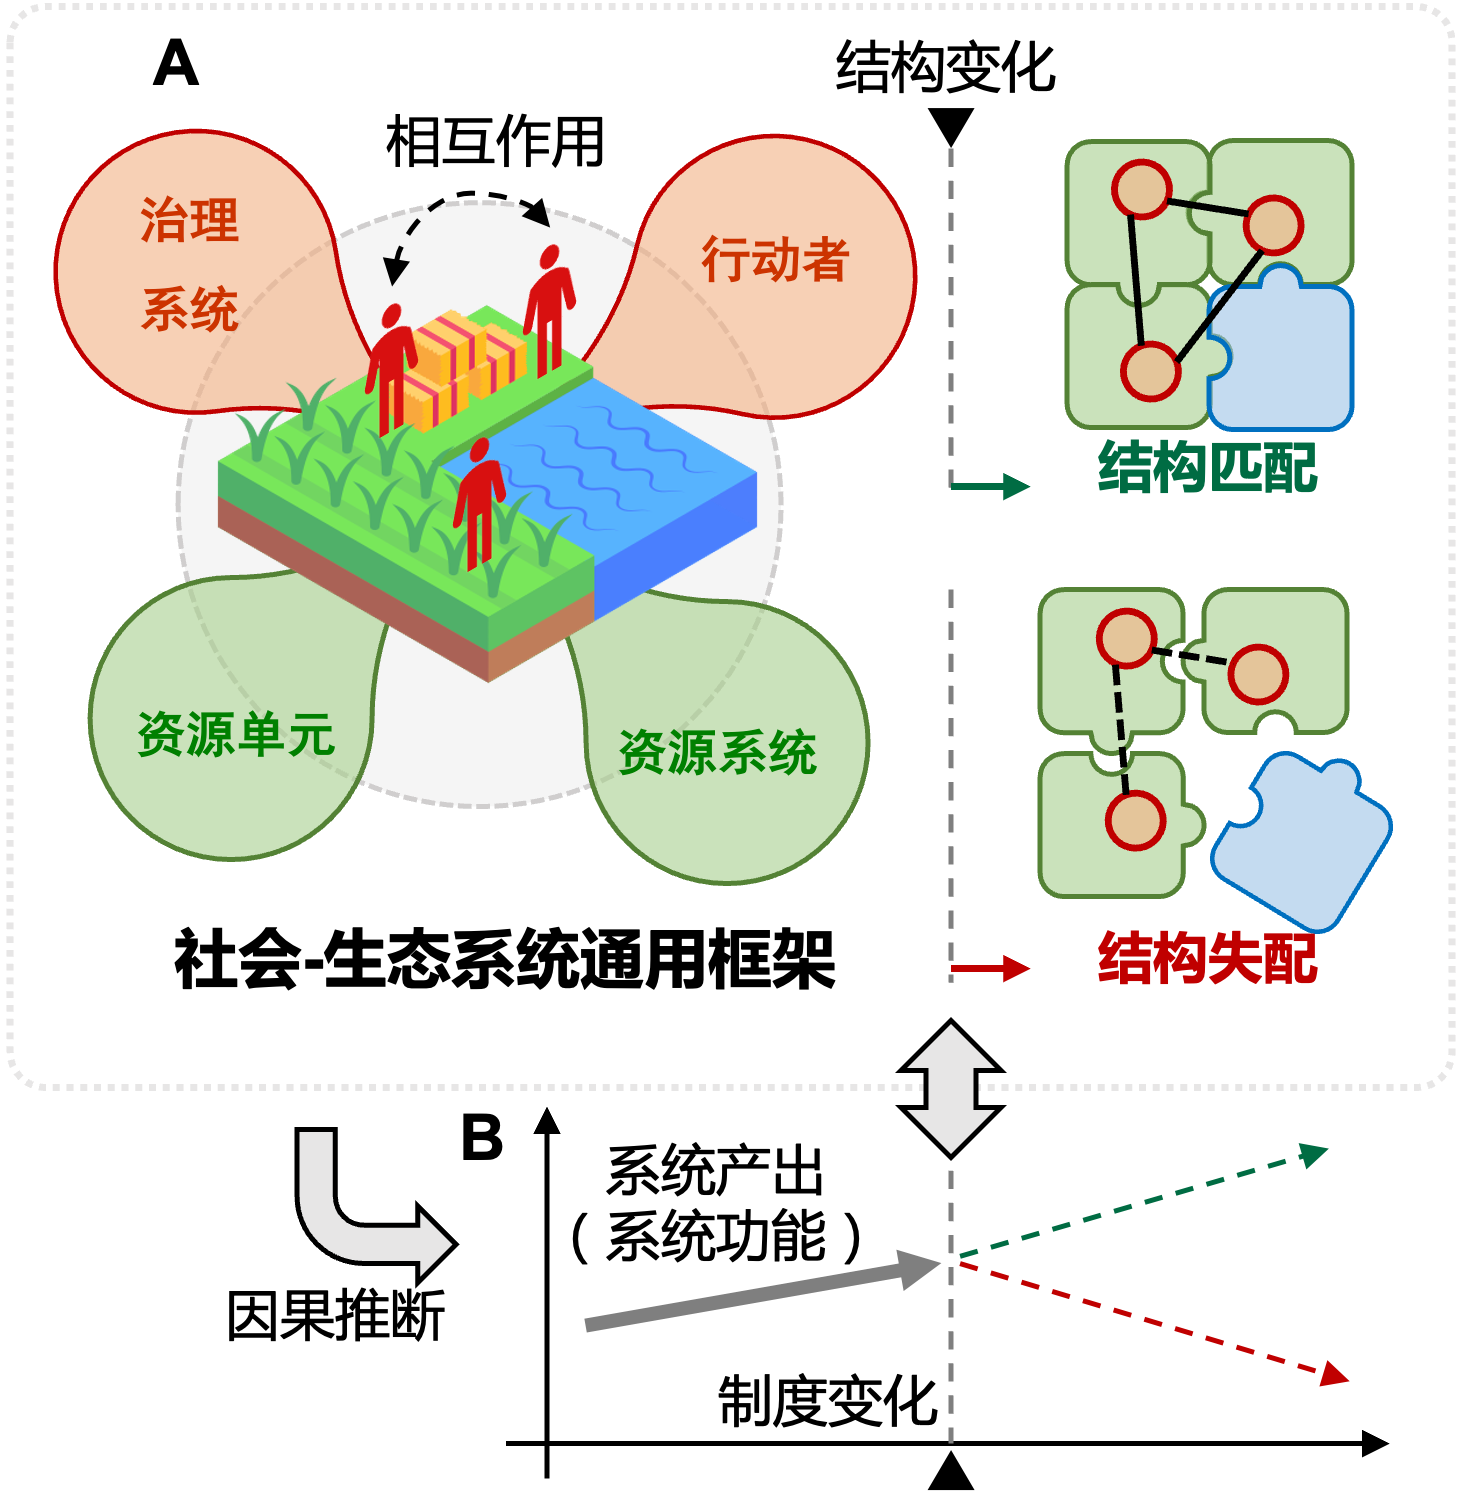
\includegraphics[width=0.6\textwidth]{img/ch5/ch5_framework.png}
    \caption[社会\textendash{}生态系统结构和结果之间的因果推断框架]{社会\textendash{}生态系统结构和结果之间的因果推断框架。\textbf{A}分析社会\textendash{}生态系统的通用框架(改编自 Ostrom, 2009~\cite{ostrom2009})内,制度变化可以通过改变系统内部的相互作用重塑结构。\textbf{B}通过构建反事实推断,可以分析匹配或不匹配的社会\textendash{}生态系统结构如何影响系统演变。}\label{fig:framework}
\end{figure}

\subsection{数据与预处理}\label{sec:dataset}

为构建反事实推断模型,需要选择表征实际用水情况的因变量,以及能够用以预测地区用水量的自变量。
本章研究从国家水利部开展的用水量调查数据作为观测值,从不同来源获取了农业、工业、服务业、居民生活、环境五个类别共计$24$个影响区域用水的社会、经济、环境因素作为自变量\cite{zhou2020}(见表~\ref{ch5:tab:data_source})。
数据集的空间范围包括中国$30$个省、自治区、直辖市和地区(不包括台湾、香港、澳门;天津和河北因在分水政策中被合在一起考虑,因此合并两地数据为“津冀”)。
数据集的时间范围涵盖两次政策前后各十年,即$1979$年至$2008$年,数据所有特征在该时间段内均无任何缺失值。

% Table generated by Excel2LaTeX from sheet '数据来源'
\begin{table}[htbp]
    \caption{推断地区用水量的自变量数据}
      \begin{tabularx}{\textwidth}{LLLL}
      \toprule
      \multicolumn{1}{l}{部门} & 分类    & 单位    & 描述 \\
      \midrule
      \multicolumn{1}{l}{农业$^1$} & 灌溉面积  & 千公顷   & 装配了灌溉设施的不同作物面积 \\
      \multicolumn{1}{l}{工业$^2$} & 产值    & 千百万元  & 工业各产业的总增加值 \\
            & 循环用水比例 & \%    & 工业循环用水占总用水比例 \\
      \multicolumn{1}{l}{服务业} & 服务业总增加值 & 百万元   & 服务业的总增加值 \\
      \multicolumn{1}{l}{居民生活} & 城市人口  & 百万人   &  \\
            & 农村人口  & 百万人   &  \\
            & 牲畜数量  & 十亿千焦  & 牲畜卡路里总和 \\
      \multicolumn{1}{l}{环境} & 气温    & K     & 近地表气温 \\
            & 降水量   & mm    & 年累计降水量 \\
      \bottomrule
      \end{tabularx}\label{ch5:tab:data_source}%
      \footnotesize
      1. 包括以下作物类型:水稻、小麦、玉米、水果、其它
      2. 包括以下产业:纺织、造纸、石油化工、冶金、采矿、粮食生产、水泥、机械、电子、电力、其它
\end{table}%
  

在``八七''分水方案和流域统一调度均涉及的$10$个省份或地区中,四川、津冀因为从黄河流域取用水占该地区总用水量不足$5\%$而不作为“受政策影响区域”被剔除(见表~\ref{ch5:tab:quota})。
由于数据的量级和单位相差较大,为便于后续研究,在进行分析前统一对数据集的所有特征进行标准化(见式\ref{ch5:eq:normalization})。
\begin{equation}
    x_{\textit{normalized}}=\frac{x-\bar{x}}{s}
    \label{ch5:eq:normalization}
\end{equation}

其中,$x_i$ 表示第 $i$ 个数据,$\bar{x}$ 表示数据的均值,$s$ 表示标准差。

此外,提出与实施分水制度的直接原因是解决黄河$1972$年以来的断流问题\cite{wang2019b},本文还使用了研究时段内的黄河断流数据(包括断流的天数和河段长度)和流域的平均干旱指数数据\cite{wang2022e}。

\subsection{主成分分析}

主成分分析(Principal Components Analysis, PCA)是一种用于降低大型数据集维度的技术,该方法利用原始变量的线性组合创建了一个新的变量集,这些新的变量被称为主成分(PC)。
Bayan(2021)\cite{bayani2021}已证明了将主成分分析与合成控制法(Synth Control, SC)相结合可以提高其因果推理的鲁棒性。
面板数据不能直接应用主成分分析,因此本章研究将所有预处理后的数据沿时间轴进行多年平均,对均值使用主成分分析进行降维,将得到的主成分按照其在原始数据中解释方差变化的大小顺序进行排序,并用肘部法确定主成分的个数,从而降低反事实推断合成控制模型的自由度。

负荷率代表每个原始变量与主成分之间的相关性,通过原始变量在每个主成分上的负荷,可以分析对区域用水量贡献最大的主成分与特征集合有关,了解用水量影响特征与主成分的相互关系。
参考 Mirco 等人的研究,每个特征对于特定主成分的贡献是否显著主要有三种方法:特征向量法、负荷阈值法、固定阈值法~\cite{migliavacca2021}。
本章研究采用负荷阈值法分析各特征对不同主成分的贡献,即当负荷值的绝对值和贡献大于与维数(即变量)相关的特定阈值时(即$|{x_{loading}}| > 1/N_{dims}$),认为该特征对当前主成分的贡献显著。


\subsection{差分合成控制}\label{sec:DSC}

本章研究选用差分合成控制法(Differenced Synthetic Control, DSC)构建反事实推断模型,估算不受制度变化影响情景下的流域用水量,从而对分水制度的影响进行因果推断(Causal Inference)。
DSC 方法是对合成控制法(Synthetic Control, SC)在鲁棒性上的改进\cite{billmeier2013, smith2015},这一类因果推断方法可以构建一个可比的控制单元来估计历史事件或政策干预对真实单元(如城市、地区和国家)的影响及其变化趋势\cite{abadie2010, abadie2015, hill2021}。
将经降维处理的数据集分为反事实推断所需的“实验组”和“对照组”数据,其中水配额制度涉及的省份数据作为目标组$(n=8)$数据,其他省份则作为对照组$(n=20)$数据。
该方法旨在评估政策变化的影响,而这些政策变化集中在其中一些单元上。
在本研究中即为分水制度涉及的省份属于政策影响的单元,称之为“处理单元”,其用水特征作为“真实值”使用“目标组”数据的因变量进行表达。
合成控制法通过重新加权非处理单元构造其凸组合作为控制组,并匹配处理单元和控制单元在政策干预前的变化趋势构成反事实推断,处理单元和控制单元在政策干预后的因变量差异便可估计为政策干预的净效应。

本章研究中,所有处理单元(即制度涉及的诸省)都在1987年和1998年先后受到两次不同的制度干预,因此每个政策干预前后十年都被视为单独的分析时期,即一次构建反事实推断模型的研究时段可能为 1979 \textendash{} 1998(1987年为政策干预时点)或 1987 \textendash{} 2008(1998年为政策干预时点)。
接下来将黄河流域分水制度涉及的每个省份分别作为处理单元($n=8$,见\nameref{sec:dataset}),其余的$J=20$个控制单元均来自流域外未受“政策干预”的省份构建模型,这种多处理单元的合成控制法也已广泛应用\cite{abadie2021}。
% 然后,本研究认为在第$T = {1,2 \ldots , T}$时间段观测到的第$J+1$个单位。
本研究定义$T_0$为政策干预前的周期数(年份,$1,\ldots,t_0$),定义$T_1$为政策干预后的周期数($t_0,\ldots,T$),使得$T = T_0+ T_1$,每个处理单元在政策干预后的时间$T_1$内都面临制度变迁,在之前的$T_0$时期不受政策干预的影响。
控制单元的任何加权组合都是一个潜在的合成控制模型,可以用一个权重为$\mathbf{W} = (w_{1},\ldots,w_{J}), w_j \in (0, 1)$的向量$J * 1$来表示。
通过引入$k * k$的对角线半定矩阵$\mathbf{V}$表示各协变量相对重要性,那么在所有潜在合成控制模型中求解最优合成控制权重$W$的过程为:

\begin{equation}
    \mathbf{W^{*}(V)}=\underset{\mathbf{W} \in \mathcal{W}}{\operatorname{minimize}}{\left(\mathbf{X}_{\mathbf{1}}-\mathbf{X}_{\mathbf{0}} \mathbf{W}\right)}^{\prime} {\mathbf{V}}{\left(\mathbf{X}_{\mathbf{1}}-\mathbf{X}_{\mathbf{0}} \mathbf{W}\right)}
\end{equation}

给定$\mathbf{V}$的情况下,$\mathbf{W}$是矩阵$\mathbf{W}^{*}(V)$的权重向量,使处理单元与控制单元之间的特征差异最小。
这意味着$\mathbf{W^{*}}$取决于对$\mathbf{V}$的选择,因此可以用$\mathbf{W*(V)}$表示。
差分合成控制法选择$\mathbf{V^{*}}$作为优化$\mathbf{W*(V)}$的$\mathbf{V}$,通过让政策干预单元和合成控制法构建的对照单元在政策干预前的结果差异最小化:

\begin{equation}
    \mathbf{V}^{*}=\underset{\mathbf{V} \in \mathcal{V}}{\operatorname{argmin}}{\left(\mathbf{Z}_{1}-\mathbf{Z}_{0} \mathbf{W}^{}(\mathbf{V})\right)}^{\prime}{\left(\mathbf{Z}_{1}-\mathbf{Z}_{0} \mathbf{W}^{*}(\mathbf{V})\right)}
\end{equation}

其中$\mathbf{Z}_{1}$是一个$1*T_0$的矩阵,包含政策干预单元在干预前的每一个观察样本。
类似地,让$\mathbf{Z}_{0}$作为一个$k * T_0$的矩阵,其中包含了政策干预前期控制单元每个的观察结果,其中$k$为数据集中变量的数目。

\subsection{鲁棒性检验}

对合成控制法(DSC)的鲁棒性测试方法主要有两种。
首先,可以比较处理前后(本章研究中为流域分水政策的干预)对推断变量(本章研究中为用水量)的重建效果,如在处理前重建的模型预测值与实际观测值差距很小,重建后的预测值和观测值差距很大,则说明政策干预的效果非常明显。
本章研究中,为判断干预效果是否显著,使用配对样本$T$检验计算统计量,针对1987年``八七''分水方案和1987年流域统一调度两次制度干预,分别对其制度干预前期、后期的模型预测和实际观测数据进行检验。
若政策干预后的 $p$ 值小于阈值(本章研究采用置信度水平95\%,即阈值为$0.05$),则能够拒绝“两者无显著差异”的原假设$H_0$,认为制度干预让该区域用水量发生了显著变化。
若制度干预前$T$检验的显著性水平大于阈值,则说明DSC模型在制度干预前成功预测了该地区用水量随时间的变化,拟合效果很好。

其次,安慰剂试验是评估合成控制方法有效性的另一种常见方式。
在安慰剂试验中,用一个从控制单位库中选出的安慰剂单位代替被处理单位,然后使用与被处理单位相同的数据和参数,对安慰剂单位实施合成控制方法。
如果合成控制方法是有效的,应该在安慰剂单位和控制单位之间产生明显的差异,因为安慰剂单位不应该受到干预的影响。
安慰剂测试可以用来评估合成控制方法的有效性,并检测分析中的任何偏差或混杂因素。
本研究采用 Abadie 提出合成控制法时建议的安慰剂检验步骤\cite{abadie2010},使用 Dmitry 等人开发的差分合成控制法的 Python 库进行安慰剂检验。如果在大多数省份中,合成后期均方根误差(见式\ref{ch5:eq:RMSE})与合成前期的比率显著高于(同样采用$T$检验判断差异的显著性)其他安慰剂单位的结果,则表明在制度处理时期(1987年和1987年)黄河流域受影响比大多数其他省份影响更大。

\begin{equation}
    \label{ch5:eq:RMSE}
    \text{RMSE} = \sqrt{\frac{1}{n}\sum_{i=1}^{n}{(y_i-\hat{y}_i)}^2} 
\end{equation}

其中$n$为观测数,$y_i$为实际值,$\hat{y}_i$为预测值。

\subsection{计算方法与软件实现}

主成分分析使用了$pca$软件包(v-1.9.1)\cite{Taskesen_pca_A_Python_2020},单差分合成控制法在其作者公开的$Synthetic Control Methods$软件包基础上修改完善\cite{arkhangelsky2021}。所有库在 Python 3.11.2 环境下运行,本章研究的所有代码已公开在GitHub(https://github.com/SongshGeo/Water-Allocation-Institution)。


\section{制度的结构演变过程}\label{ch5:process}

% \subsection{INSTITUTIONAL SHIFTS AND STRUCTURES}
\subsection{分水制度与流域SES构件的演变}\label{results-1}

\begin{figure}[!t]
	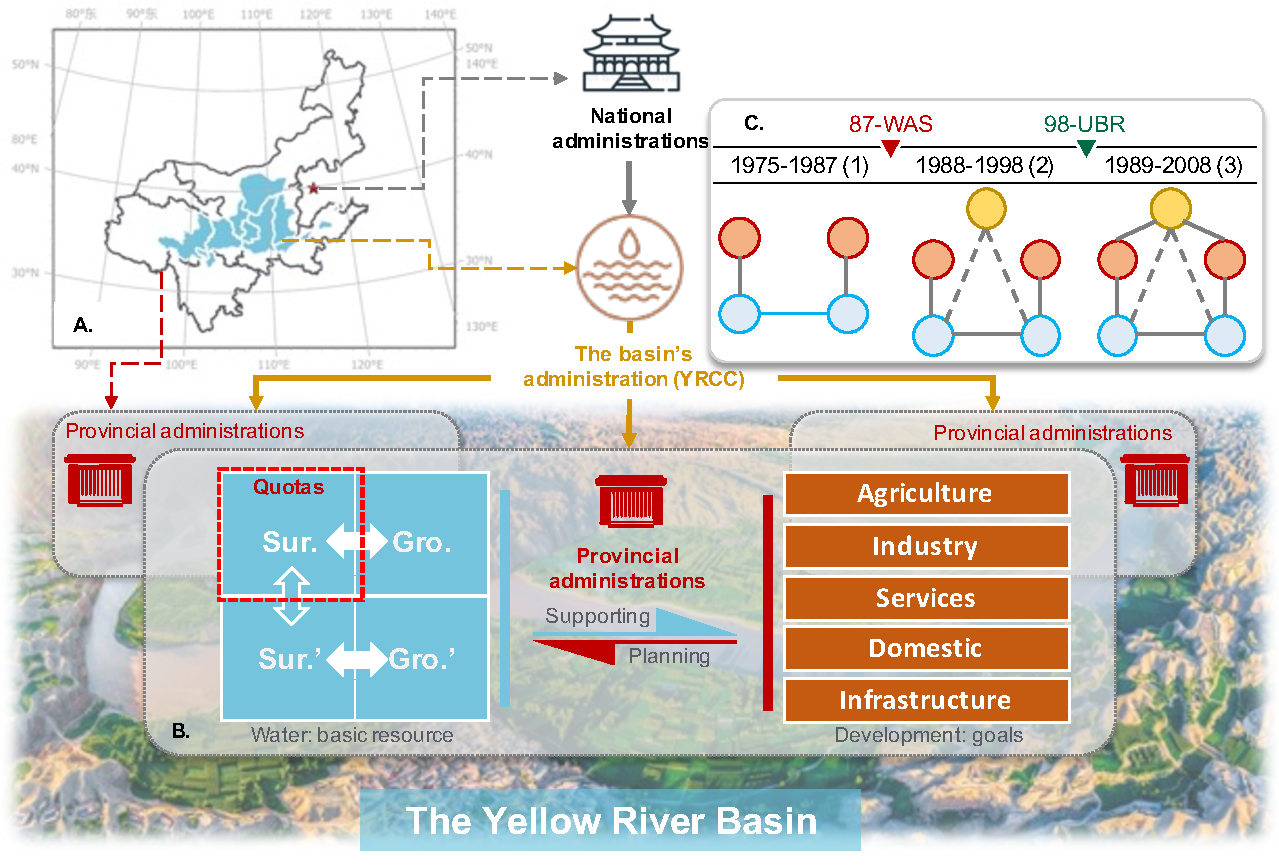
\includegraphics[width=\linewidth]{img/ch5/diagram.pdf}
	\caption[黄河流域社会经济制度变迁及其结构]{
		黄河流域社会经济制度变迁及其结构。
		\textbf{A.} 黄河流域跨越$10$个省(地区),其中$8$个对黄河流域水资源的依赖程度较高。国家部委(水利部)是发布水治理政策的最高权力机构,这些政策通常由流域级机构黄河水利委员会和各省级机构执行。
		\textbf{B.} 地方省政府(水利厅、局)是水分方案中的主要的利益相关者。自“八七”分水方案以来,由于黄河地表水的取用受到配额限制,利益相关者规划和利用水资源进行发展受到影响。自然水文过程是相互联系的,尽管配额制度主要限制地表水($Sur$),也可能通过社会水文过程影响流域内地下水($Gro$)或流域外水资源($Sur'$和$Gro'$)。
		\textbf{C.} 制度变迁和随之而来的社会-生态系统结构变化:
		(1) $1979 \sim 1987$年间,各利益相关方(红圈)从连接的生态单元(黄河河段,蓝圈)自由获取水资源。
		(2) 1987年施行“八七”分水方案后,黄河水利委员会(黄圈)负责监测各河段利益相关者用水情况。
		(3) 1998年施行“流域统一调度”之后,利益相关者必须向黄河水利委员会申请用水许可证(红黄圈之间的连接)。}\label{fig:structure}
\end{figure}

% 制度变动综述
1987年实施的“八七”分水方案和1998年实施的“流域统一调度”是黄河流域水治理中被广泛认可的里程碑事件。
在“八七”分水方案之前,分水方案的利益相关者(参与分水的黄河流域各省份或地区)可以根据其取水能力自由使用黄河的水资源进行开发,流域管理机构(黄河水利委员会)与利益相关者在用水方面没有联系(图~\ref{fig:structure}~C)。
为缓解水资源压力,国家部委在“八七”分水方案中提出黄河流域$10$个省(或地区)之间应参照指定配额来取用水资源,且该配额与各省的预期取水量相去甚远(表~\ref{ch5:tab:quota})。
同时根据官方文件中的要求,流域尺度机构黄河水利委员会需开始报告各省(或地区)和各个河段的用水情况,这是黄河流域水利枢纽的责任首次涉及水资源利用,在社会与生态节点之间引入了新的联系(图~\ref{fig:structure}~C)。
由于备受争议的“八七”分水方案在此后十年内都没能解决黄河断流问题,1998年水利部签署同意了另一项制度改革——流域统一调度,强化了黄河水利委员会在综合管理用水方面的职责。
此次官方文件明确指出,各省须将其年度用水计划向黄河水利委员会报备并申请用水许可证,否则不再能使用黄河干流水资源,黄河水利委员会因此在社会-生态系统结构中同各省直接联系在一起(图~\ref{fig:structure}~C)。
综上所述,两次制度转换重塑了黄河流域水资源利用的结构,形成的三类具一般性的社会-生态系统结构块如图~\ref{fig:structure}~C所示。

% Table generated by Excel2LaTeX from sheet '八七分水方案配额'
\begin{table}[htbp]
    \caption{八七分水方案水资源配额}
      \begin{tabularx}{\textwidth}{p{2cm} LLLLLLLLLL}
      \toprule
            & \multicolumn{1}{l}{青海} & \multicolumn{1}{l}{四川$^b$} & \multicolumn{1}{l}{甘肃} & \multicolumn{1}{l}{宁夏} & \multicolumn{1}{l}{内蒙古} & \multicolumn{1}{l}{山西} & \multicolumn{1}{l}{陕西} & \multicolumn{1}{l}{河南} & \multicolumn{1}{l}{山东} & \multicolumn{1}{l}{津冀$^b$} \\
      \midrule
      规划需求  & 35.7  & 0     & 73.5  & 60.5  & 148.9 & 115   & 60.8  & 111.8 & 84    & 6 \\
      1983年方案 & 14    & 0     & 30    & 40    & 62    & 43    & 52    & 58    & 75    & 0 \\
      1987年方案 & 14.1  & 0.4   & 30.4  & 40    & 58.6  & 38    & 43.1  & 55.4  & 70    & 20 \\
      多年平均耗水$^a$ & 12.03 & 0.25  & 25.8  & 36.58 & 61.97 & 21.16 & 11.97 & 34.3  & 77.87 & 5.85 \\
      黄河水在地区总用水的占比 & 48.12\% & 0.10\% & 30.79\% & 58.45\% & 47.82\% & 73.55\% & 44.39\% & 24.77\% & 34.41\% & 3.11\% \\
      \bottomrule
      \end{tabularx}\label{ch5:tab:quota}%
      \footnotesize
      \\
      $a$ 使用1987年到2008年数据计算,四川因数据不足,使用2004到2017年数据计算。\\
      $b$ 由于取自黄河流域的水资源占省(或地区)总用水量的比值太小($< 5\%$),不在本研究中进行考虑。
\end{table}%


\subsection{主成分提取结果}

具有解释力的变量是构建稳健的合成控制方法的关键。
我们使用了与水消耗相关的24个变量(见表~\ref{ch5:tab:data_source}),这些数据集在先前的研究中已用于解释中国水消耗的变化\cite{zhou2020}。
由于这些变量之间存在自相关性,我们使用肘部法选择了5个主成分作为DSC的输入,以减少维数并增强合成控制方法的稳健性(见图~\ref{fig:elbow})。

\subsection{合成控制结果}

对DSC的有效性测试有两种方法:(1)比较后期和前期的重建;(2)通过安慰剂分析测试鲁棒性。
对于(1),每个省份和它们的合成后期差异显著,而在合成前期差异较小(见图~\ref{fig:87panel}和图~\ref{fig:98panel}),这表明其水消耗变化的估计重建良好。
对于(2),我们采用了\cite{abadie2010}所描述的现场安慰剂分析。在大多数省份中,合成后期MSPE与合成前期MSPE的比率高于其他安慰剂单位的中位数,这表明在治疗时间(此处为1987年和1998年)发生的制度转变比大多数其他省份影响更大(见图~\ref{fig:87placebo},图~\ref{fig:98placebo}和表~\ref{tab:DSC_summary})。


\begin{table*}
	\caption{Pre and post treatment root mean squared prediction error (RMSPE) for YRB's provinces}
	\label{tab:DSC_summary}
	\scriptsize
	\centering
	\resizebox{\linewidth}{!}{
	\begin{tabular}{lrrrrrrrr}
	\hline
	 & \multicolumn{4}{c}{1987-WAS} & \multicolumn{4}{c}{1998-UBR} \\
	 Provinces & Pre-RMSPE & Post-RMSPE & Ratio & Significant$^a$ & Pre-RMSPE & Post-RMSPE & Ratio & Significant$^a$ \\
	 \hline
	 Qinghai & 0.016 & 0.231 & 14.606 & True & 0.230 & 1.170 & 5.096 & True \\
	Gansu & 0.056 & 1.307 & 23.265 & True & 0.244 & 0.841 & 3.448 & True \\
	Ningxia & 0.097 & 0.944 & 9.697 & True & 0.332 & 1.091 & 3.284 & True \\
	Neimeng & 0.335 & 3.846 & 11.479 & True & 1.320 & 1.183 & 0.896 & False \\
	Shanxi & 0.208 & 0.675 & 3.241 & False & 0.264 & 0.401 & 1.520 & False \\
	Shaanxi & 0.181 & 0.572 & 3.164 & False & 0.096 & 0.724 & 7.579 & True \\
	Henan & 0.210 & 3.207 & 15.292 & True & 1.222 & 2.479 & 2.029 & False \\
	Shandong & 0.209 & 1.840 & 8.785 & True & 0.431 & 1.517 & 3.516 & True \\
	\hline
	\end{tabular}}
	\footnotesize[a]\leftline{{Larger post/pre RMSPE than the median of the placebos.}}\\
\end{table*}



\begin{figure}[!bh]
    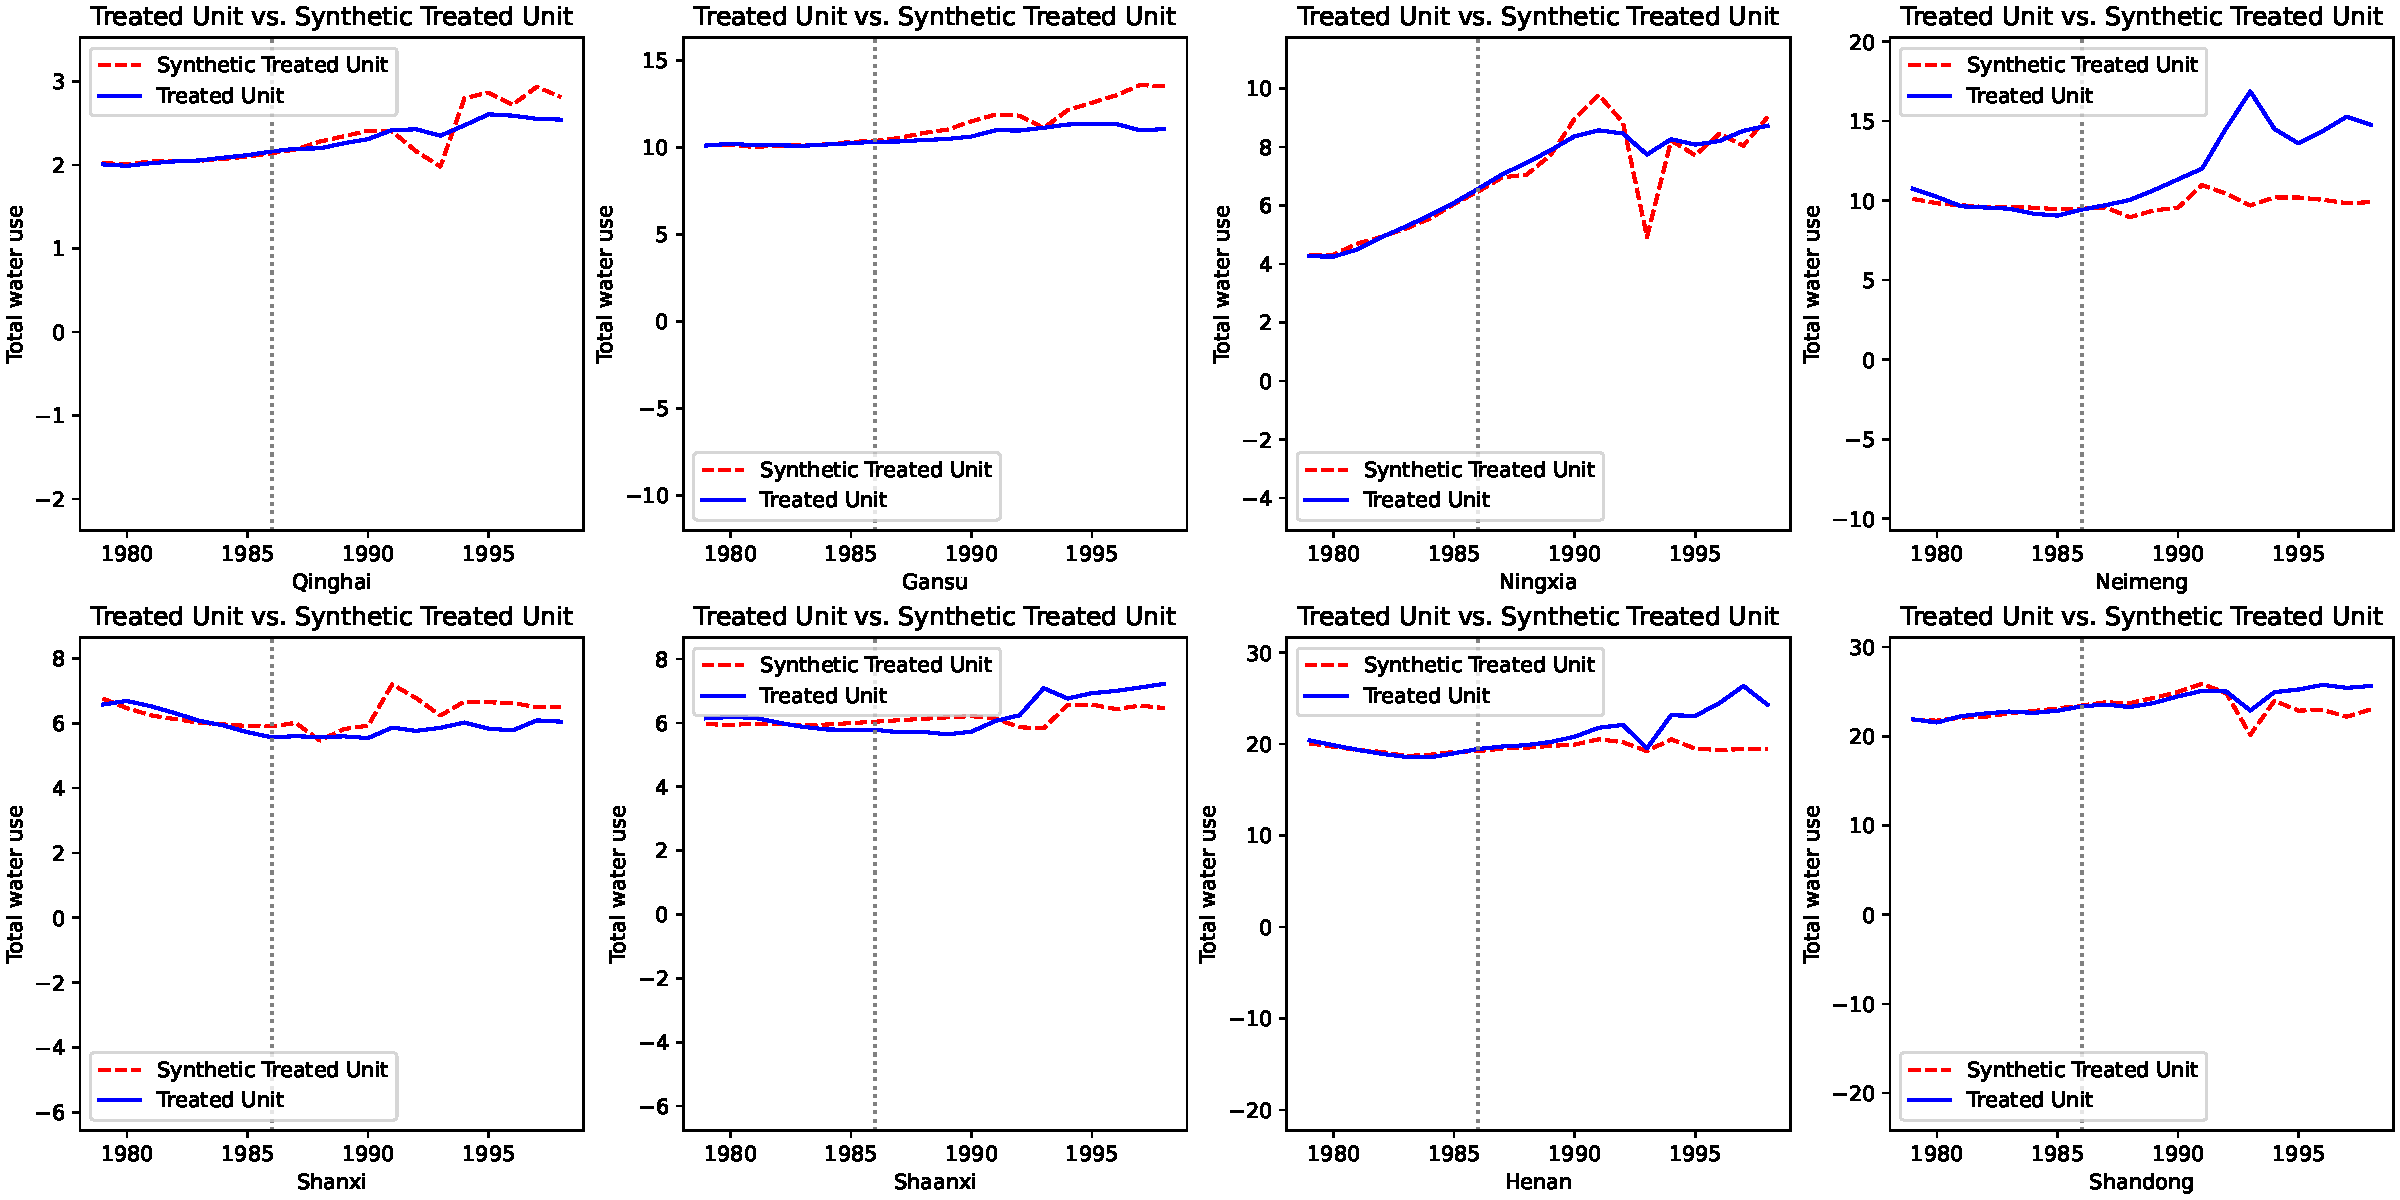
\includegraphics[width=0.9\linewidth]{img/ch5/87panel.pdf}
    \centering
    \caption{Comparations between YRB' provinces and their synthetic controls around the 87-WAS.}\label{fig:87panel}
\end{figure}

\begin{figure}
    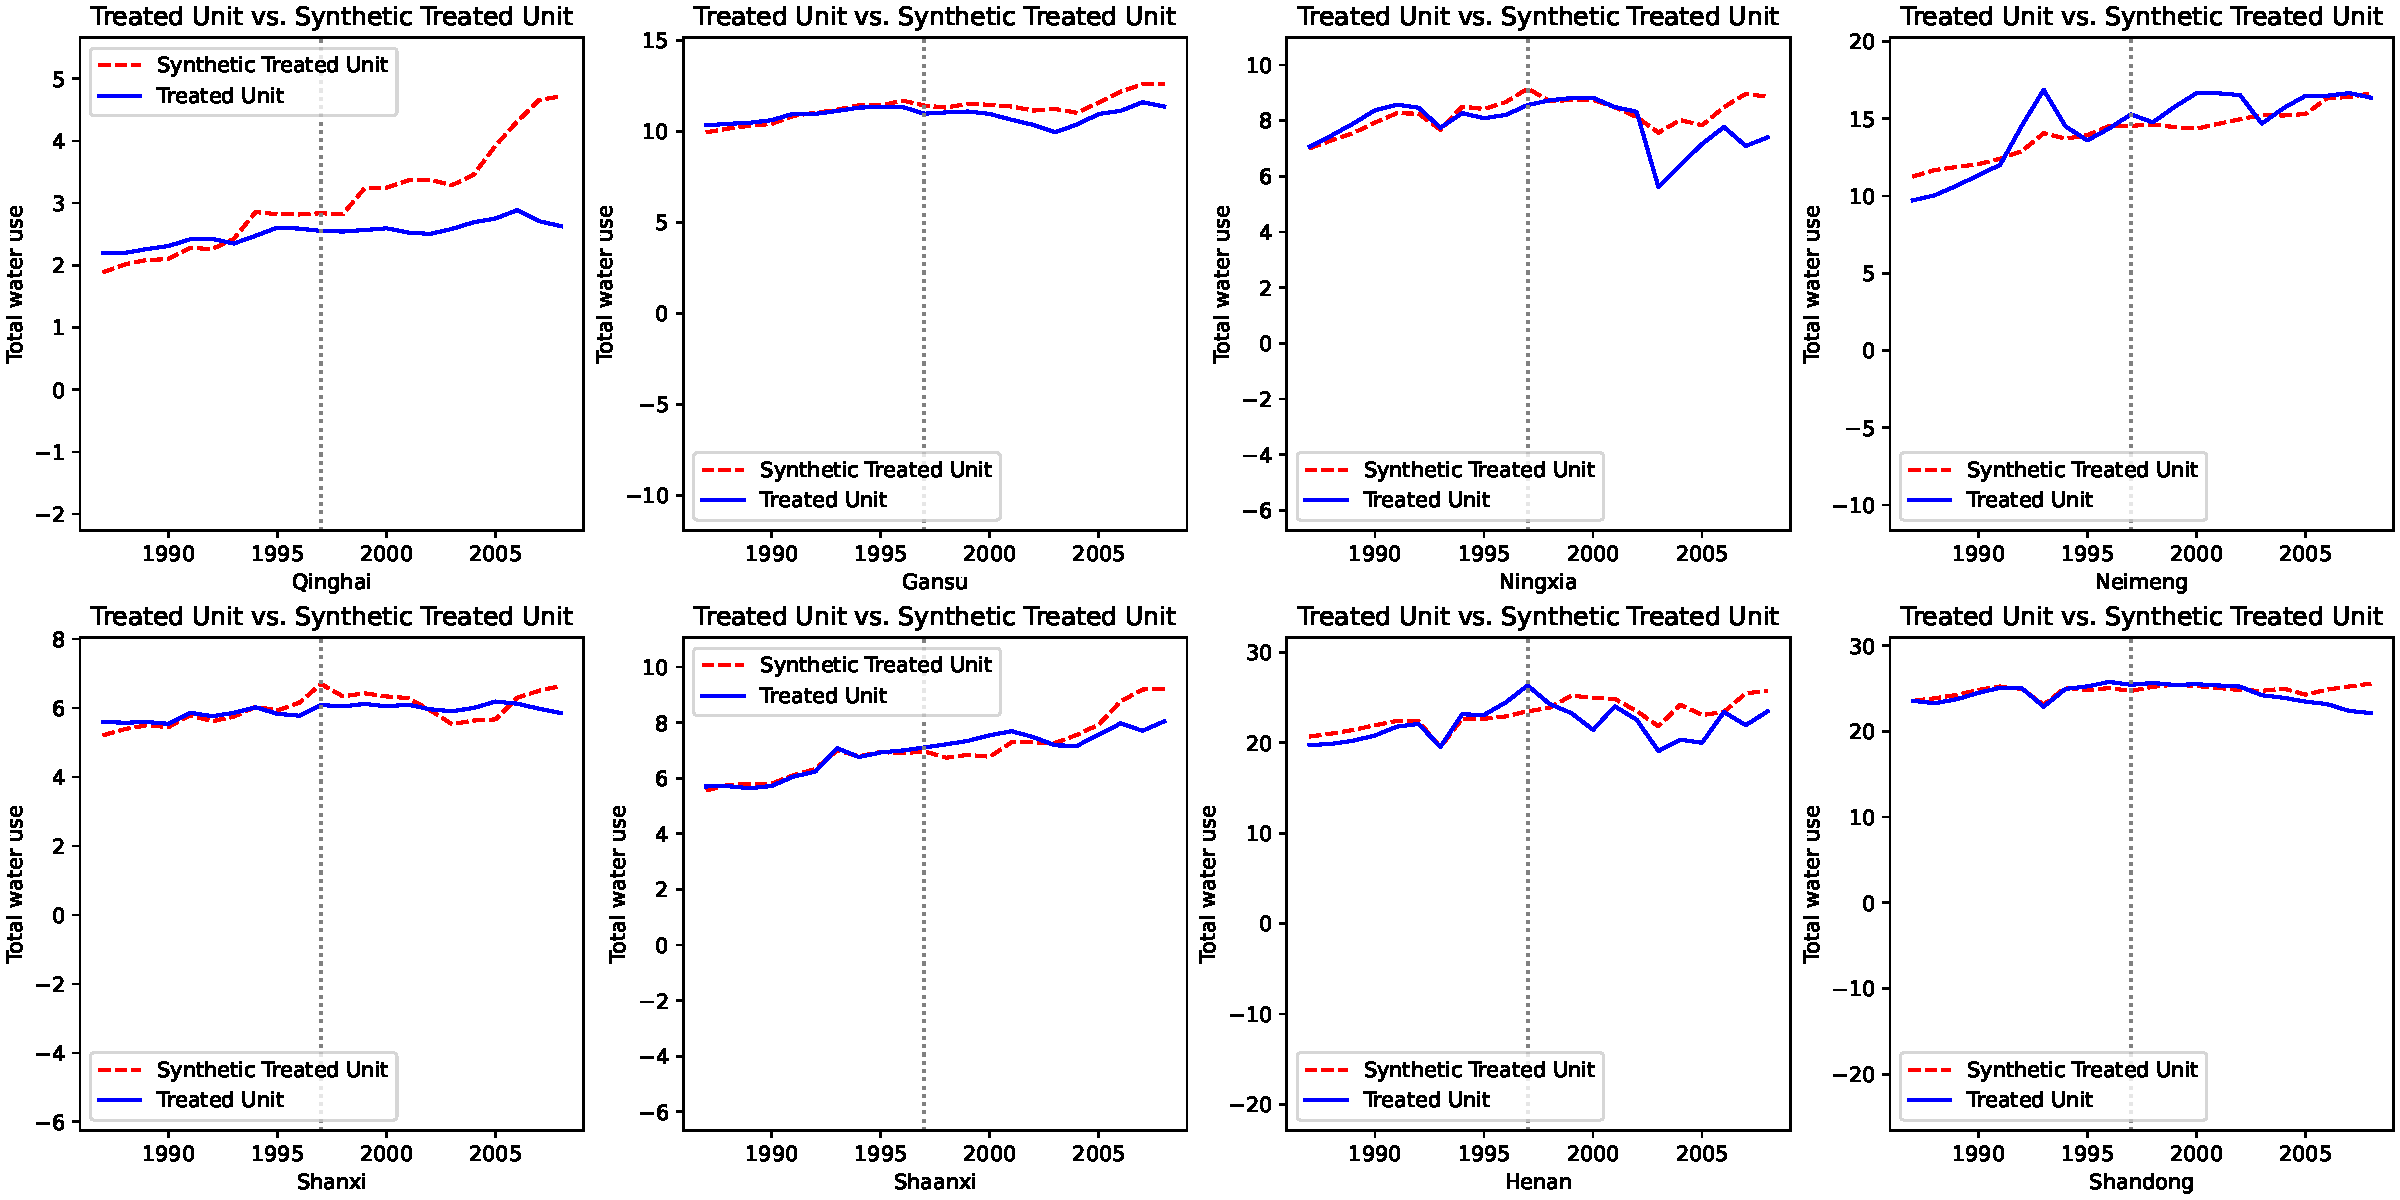
\includegraphics[width=0.9\linewidth]{img/ch5/98panel.pdf}
    \centering
    \caption{Comparations between YRB' provinces and their synthetic controls around the 98-UBR.}\label{fig:98panel}
\end{figure}


\begin{figure}
    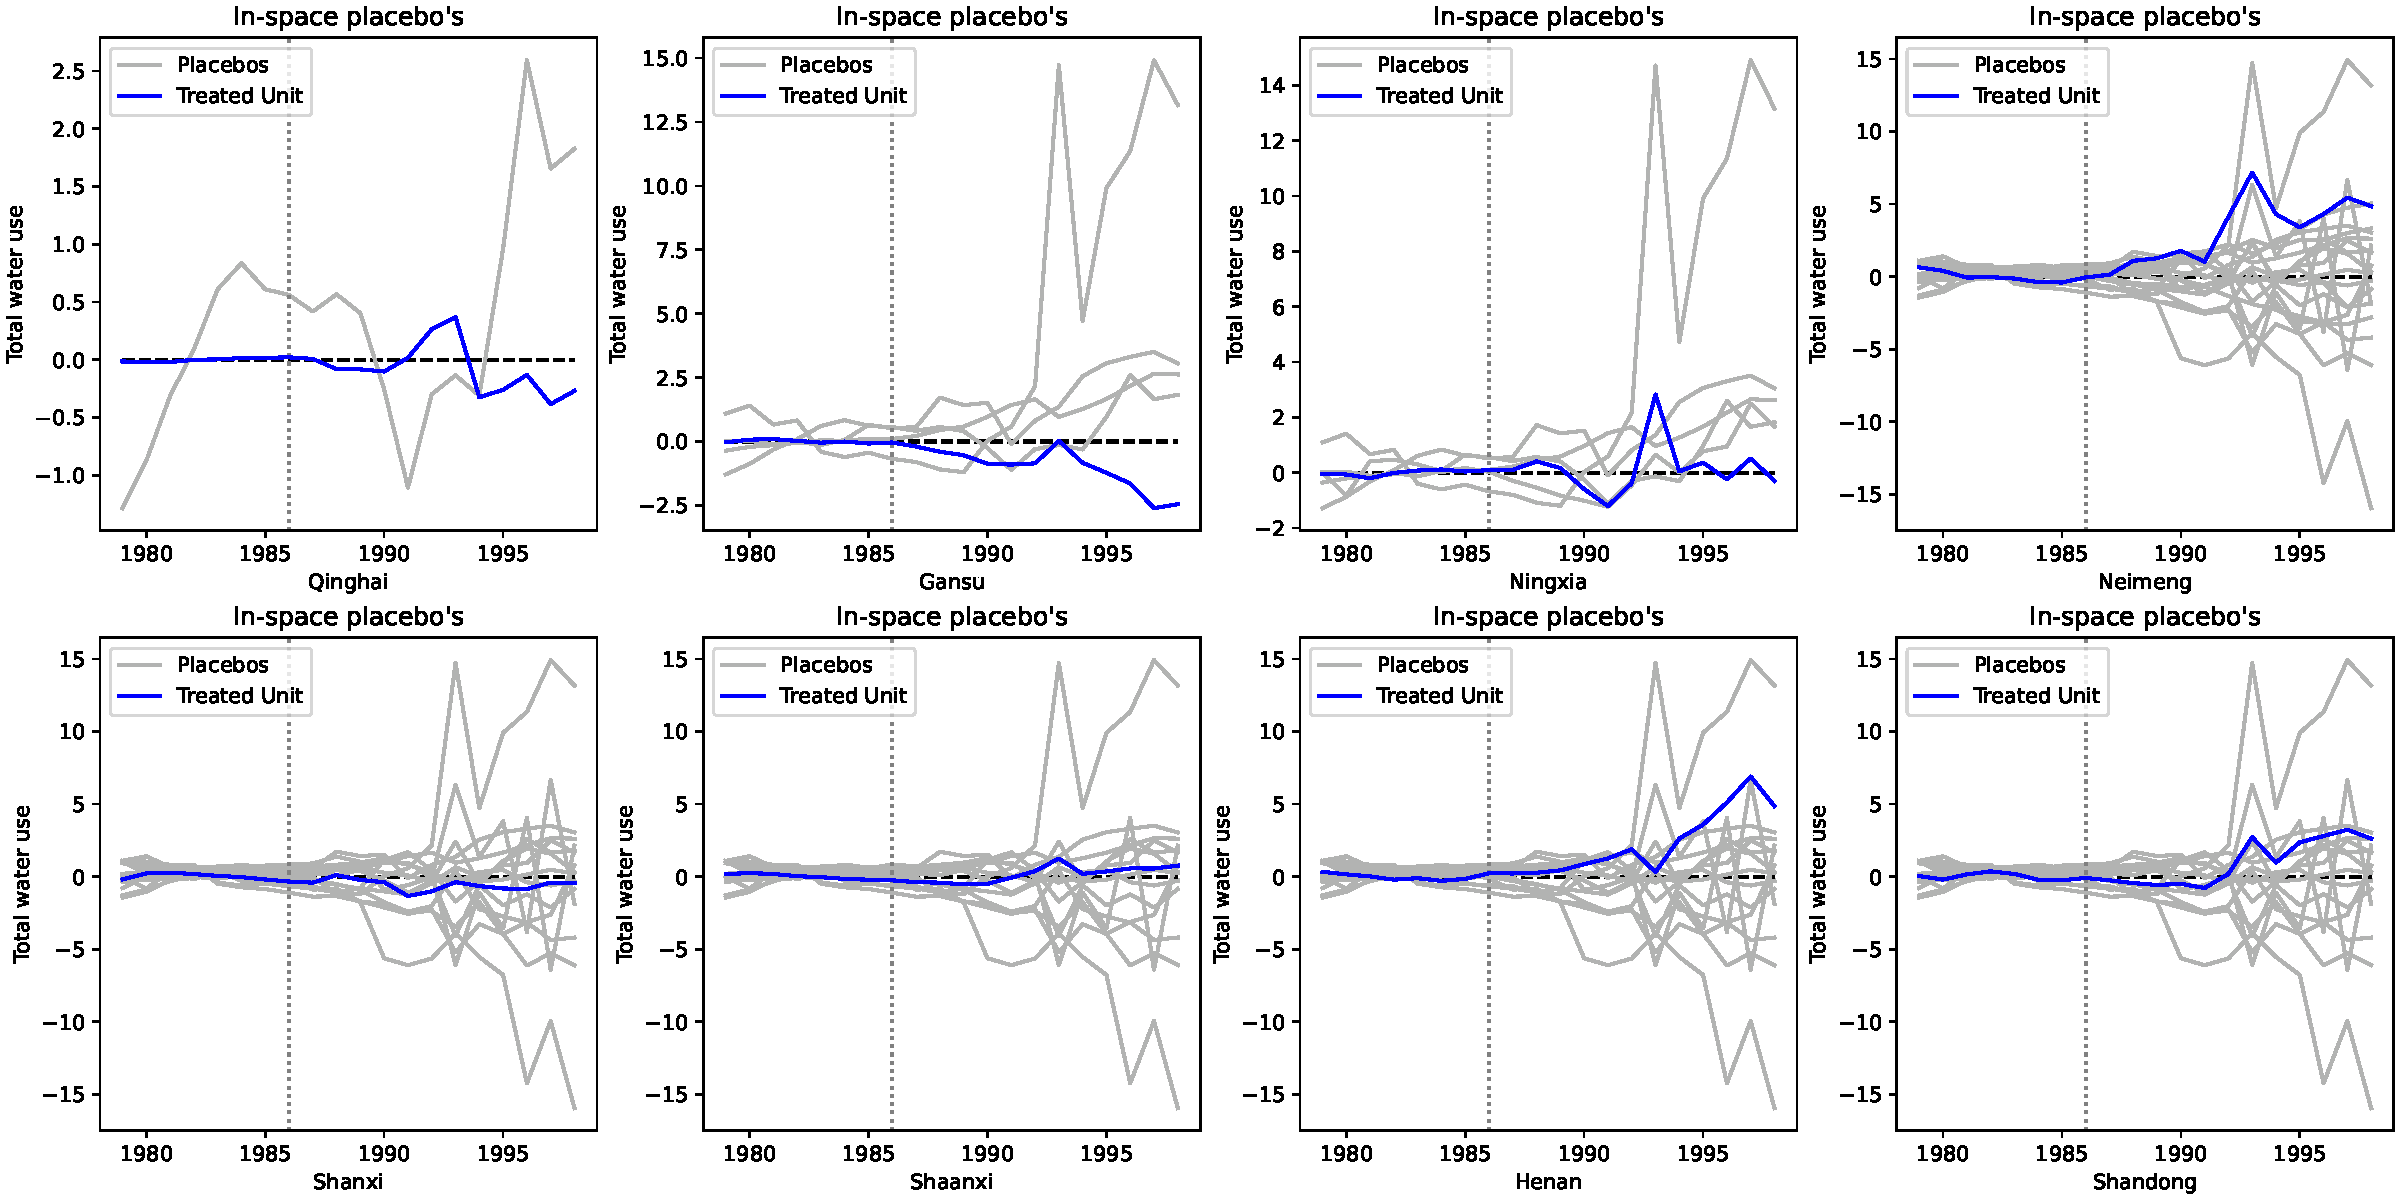
\includegraphics[width=0.9\linewidth]{img/ch5/87placebo.pdf}
    \centering
    \caption{Gaps in change in water use between provinces outside the YRB and their synthetic control, around the 87-WAS, excluding the provinces with high pre-treatment RMSPE (more than $3$ times of treated units' RMSPE).}\label{fig:87placebo}
\end{figure}

\begin{figure}
    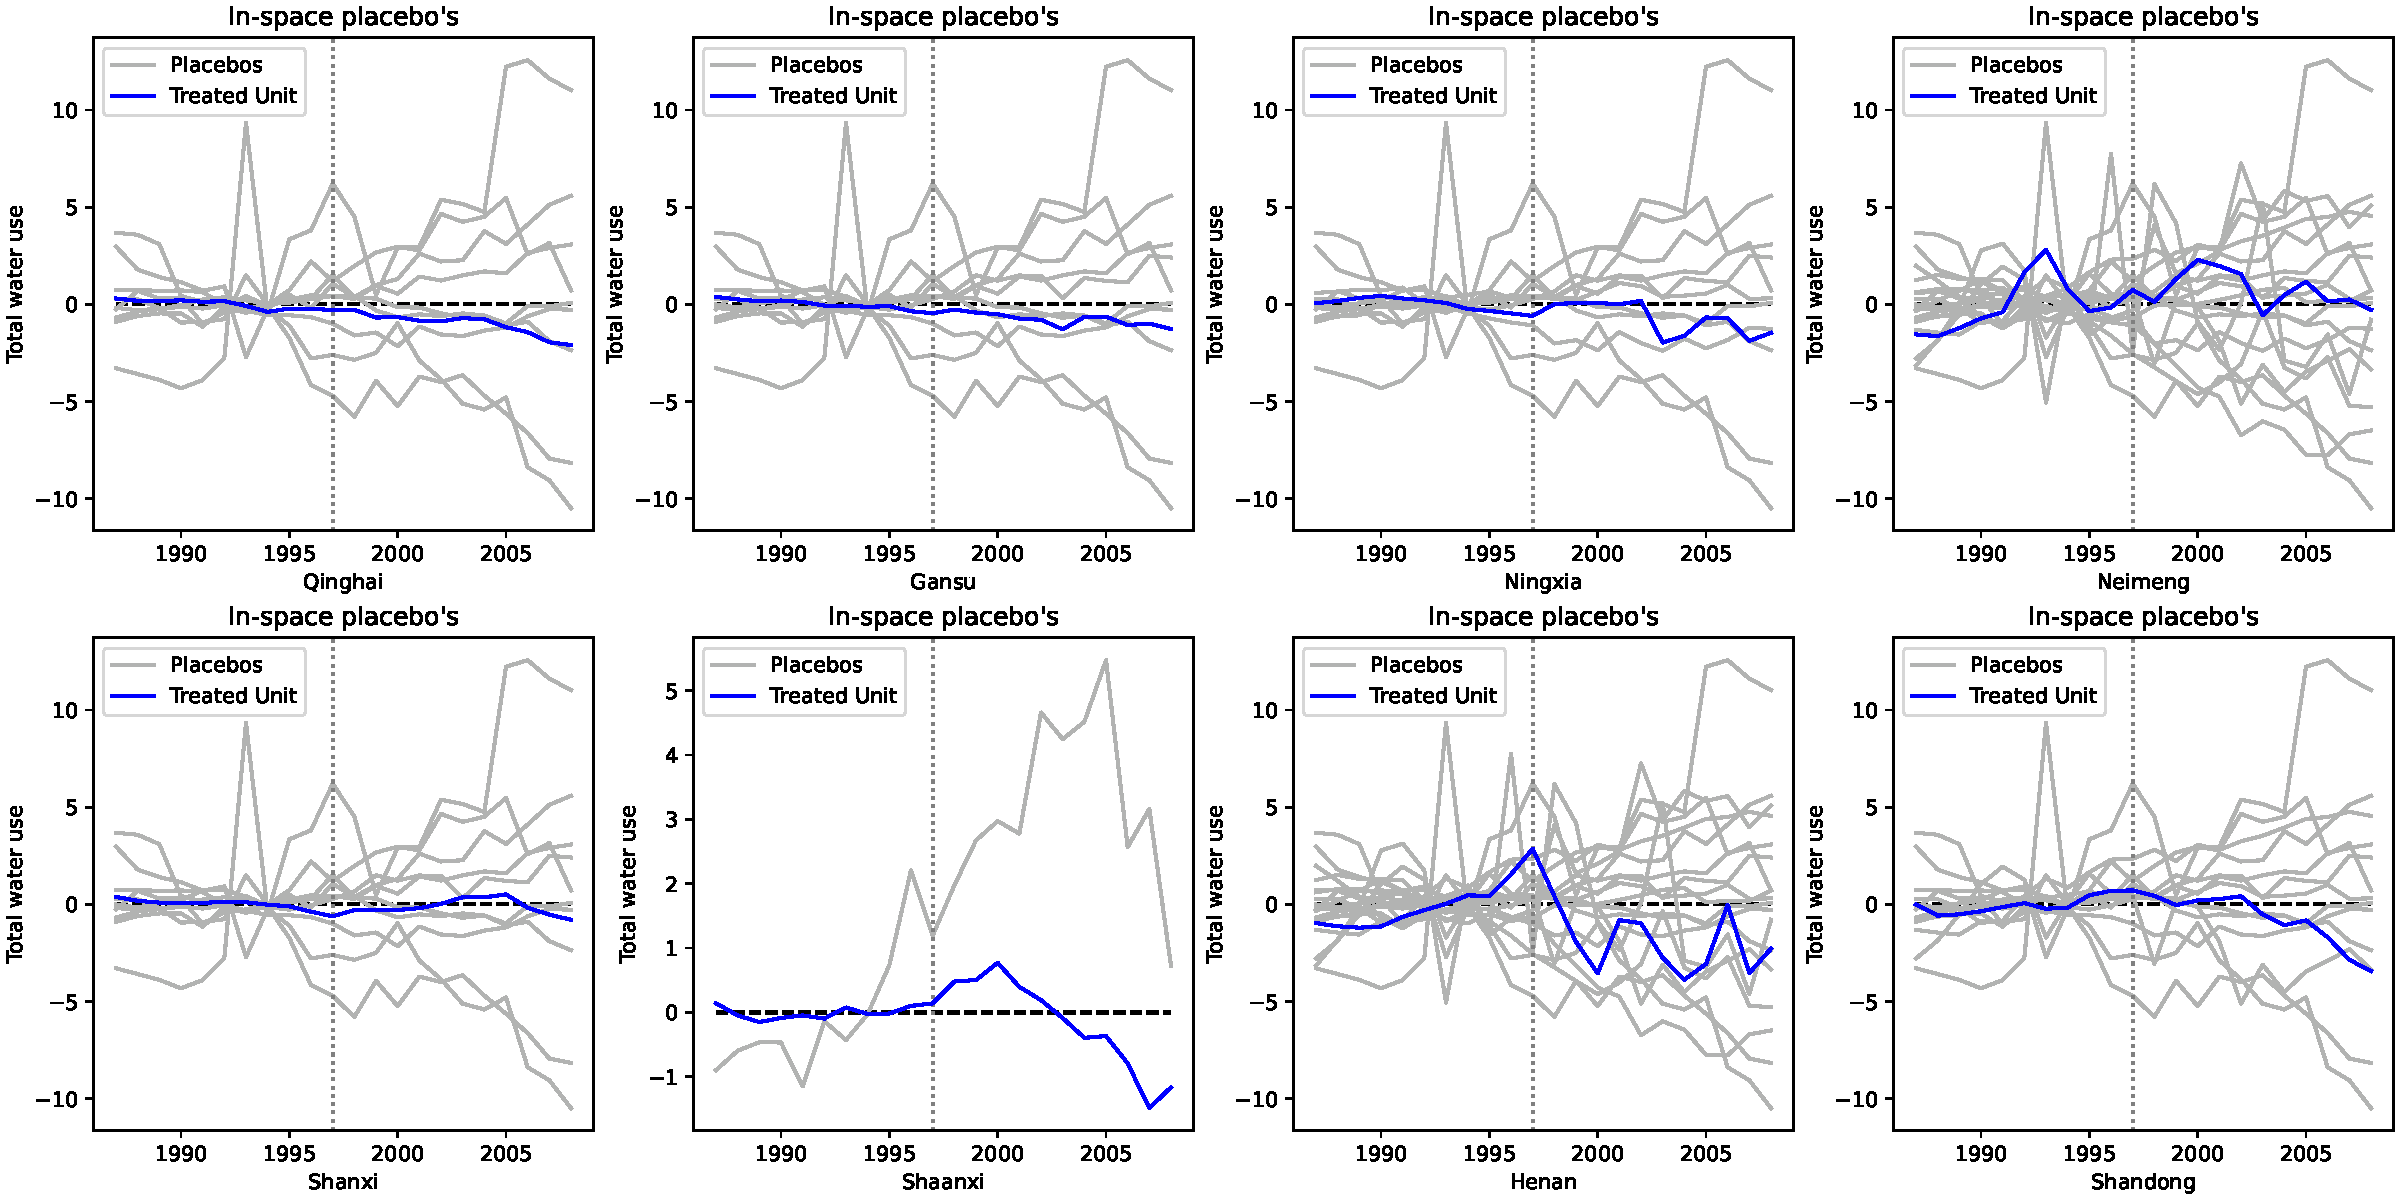
\includegraphics[width=0.9\linewidth]{img/ch5/98placebo.pdf}
    \centering
    \caption{Gaps in change in water use between provinces outside the YRB and their synthetic control, around the 98-UBR, excluding the provinces with high pre-treatment RMSPE (more than $3$ times of treated units' RMSPE)}\label{fig:98placebo}
\end{figure}


\section{制度变化对流域用水的影响}\label{ch5:mechanism}
\subsection{制度变迁对用水的影响}\label{result-2}
% 结果一:展示制度转变带来的用水量变化

\begin{figure}[!htb]
	\centering
	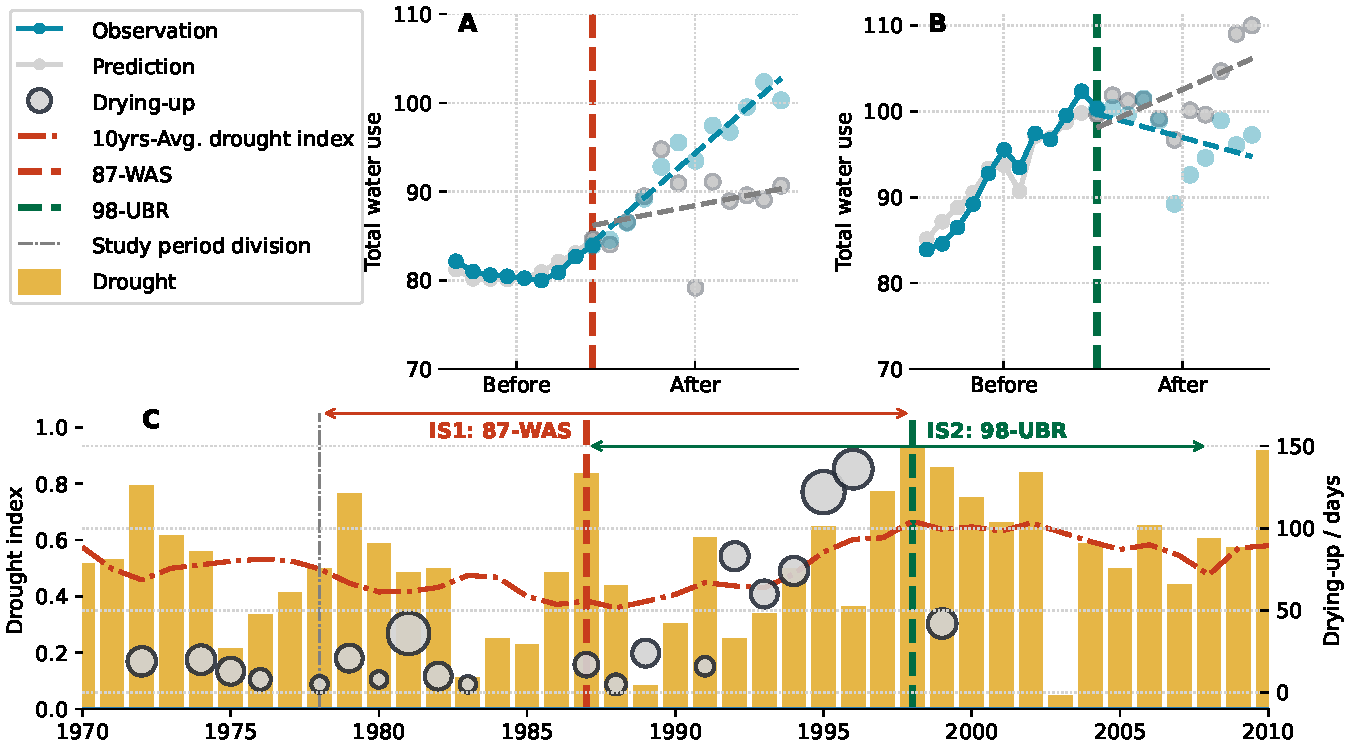
\includegraphics[width=\linewidth]{img/ch5/main_results2.pdf}
	\caption[两种制度变迁对黄河流域水资源利用与配置的影响]{
        两种制度变迁对黄河流域水资源利用与配置的影响
        \textbf{A.} “八七”分水方案前后黄河流域用水量;
        \textbf{B.} 流域统一调度前后黄河流域的用水情况。蓝线是来自统计资料的用水量,灰色线为经济和环境背景控制下差分合成控制法的估计值;
        \textbf{C.} 黄河流域干旱强度与断流事件,灰色气泡的大小表示断流河段的长度。
	}\label{fig:main_results}
\end{figure}

对用水量的理论估计表明,“八七”分水方案的制度转变促使各省取用了更多的水资源(图~\ref{fig:main_results}~A),1988年至1998年,反事实推断模型所估计的各省总用水量仅为$9743.4$亿立方米,但统计实际值达到了$10383.6$亿立方米(增加了$6.57\%$)。
在1998年流域统一调度制度出台后,用水量持续增加的趋势得到了抑制,从1998年到2008年,统计实际总用水量以每年$4.9$亿立方米的速度减少,而反事实推断所估计的用水量以$8.2$亿立方米每年的速度增加(图~\ref{fig:main_results}~B)。
“八七”分水方案后用水量的增加与$1987 \sim 1998$年日益严重的黄河断流相一致,无论是断流时长还是断流河段长度都在此时期内持续增加,导致流域生态退化和环境危机(图~\ref{fig:main_results}~C)。
尽管$1998 \sim 1987$年黄河流域的平均干旱强度还高于$1987 \sim 1998$年(平均干旱指数从“八七”分水方案后的$0.47$提升至流域统一调度后的$0.62$,图~\ref{fig:main_results}~C),1998年提出的流域统一调度却立竿见影地结束了长达二十余年的河流断流。

%\subsection{REGIONAL DIFFERENCES IN RESPONSES TO INSTITUTIONAL SHIFTS}
\subsection{对制度变化的响应差异}\label{result-3}

\begin{figure}[!htb]
	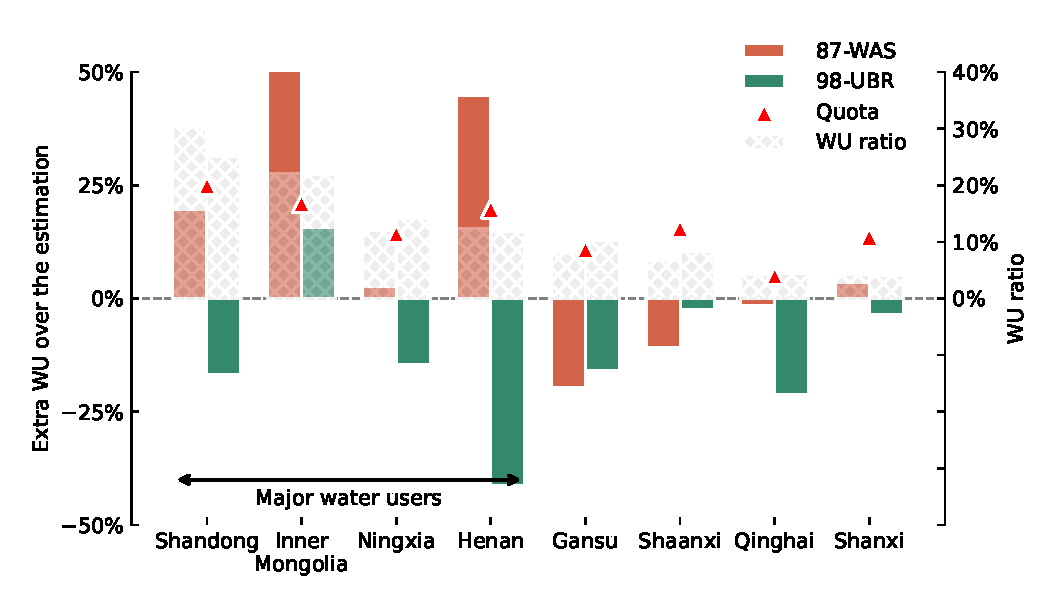
\includegraphics[width=\textwidth]{img/ch5/fig3.pdf}
	\caption[黄河流域各省份对制度变化的响应差异]{黄河流域各省份对制度变化的响应差异。红色柱状图(“八七”分水方案)和绿色柱状图(流域统一调度)分别表示在此次制度转变后的十年内,实际用水量相对于反事实推断模型估计值的增减比例。灰色柱状图显示了在两次制度转变后的十年那,各省实际用水量相对于其总用水量的比例。三角形标记指示“八七”分水方案为该省制定的理论水资源配额所占黄河流域总可用水量的比值。}\label{fig:regulating}
\end{figure}

% 结果2部分:展示区域相应差异
研究结果还表明各省(或地区)对这两次水资源分配制度改革(“八七”分水方案和流域统一调度)的响应模式存在差异。
在“八七”分水方案后的十年间,各省用水量相对反事实推断模型所估计用水量增加(或减少)的比例与其当前从黄河流域的取用水占比显著正相关(偏相关系数为$0.77$, $p<0.05$,图~\ref{fig:regulating})。
从1987年到1998年,一些用水大省(如内蒙古、河南、山东)也出现了显著的用水量增加(图~\ref{fig:regulating}),山东、内蒙古、河南和宁夏四省的用水量平均比预测值高出$32.14\%$。
而在施行流域统一调度后的1998年至2008年,几乎所有省份的用水量都出现了下降(平均下降$16.54\%$),
且各省用水量与从黄河流域的取用水占比不再呈相关性(偏相关系数为$0.33$, $p>0.1$)。


\section{讨论}\label{ch5:discussion}
\label{discussion-1}
% discussion-1:
% 用水量的上升、下降-结果解读
% 制度对社会生态系统的结果产生影响在世界范围内都很普遍,
制度对社会-生态系统(SE)结果的影响在世界范围内被广泛报道,但很少有人试图量化其净效应\cite{cumming2020a}。
结果表明,流域统一调度降低了黄河流域的用水量,而“八七”分水方案增加了$8.57\%$倍。
该结果对之前的分析提出了挑战(即,表明“八七”分水方案“几乎没有实际影响”),因为从理论上讲,如果没有影响,那么黄河流域的实际用水和合成用水之间应该没有什么差距\cite{abadie2015,hill2021}。
然而,我们的分析表明,“八七”分水方案的显著净效应表明,即使在控制了环境和经济变量之后,也会有更多的用水量。
相反,流域统一调度减少了地表水竞争,因此许多研究将河流流量恢复主要归因于该制度\cite{chen2021,huangang2002,an2007}的成功引入。

\label{discussion-2}
% discussion-2: 87的增加
% 结果与制度的目的完全相反的“八七”分水方案与许多其它的SES失败治理案例类似,表明不匹配的社会生态结构可能促进了对公共资源的掠夺式开采。
上述比较表明,“八七”分水方案的结果与该制度的目的相反,与许多其他SES治理失败相似,支持不匹配的社会生态结构会恶化共同资源\cite{kellenberg2009,cai2016,barnes2019}。
“八七”分水方案之后用水量的增加与在此期间一些省份频繁争夺水资源的担忧相一致。
尽管“八七”分水方案效果不理想的原因已经被广泛讨论(如执行、可行性和公平性),然而,结构变化受到的关注有限。
我们的结果表明,“八七”分水方案后,当前用水量与变化用水量(增加或减少)之间的相关性显著(图\ref{fig:regulating})。
这种“主要用户使用更多”的模式支持这样一个假设,即分离的利益相关者(个别省份)将通过最大化效用来响应结构(在我们基于结构的模型中解释,参见图~\ref{fig:model})。

我们的理论分析的有效性得到两个事实的支持:
(1) “八七”分水方案的水配额(或初始水权)经历了利益相关者之间的“讨价还价”阶段(1982年至1987年)\cite{wang2019a, wang2019d},每个省份都试图展示其与水利用相关的发展潜力。
议价也是一个将水份额与经济总量相匹配的过程,因为主要用水户(如山东和河南)需要的水超过了他们原来的配额(如果在设计机构时仅考虑经济潜力)\cite{zuo2020}。
(2)由于决策者与利益相关者之间的信息不对称,当前用水量较高的省份在水资源分配中具有更强的议价能力。
因此,利益相关者有相当大的动机来防止水配额阻碍他们的经济潜力,这与他们向更高一级的中央政府要求更大份额的呼吁一致\cite{wang2019a, wang2019d}。

\label{discussion-3}
另一方面,社会-生态匹配也可以得到结构效应的支持。
流域统一调度后,黄河流域水利枢纽可根据气候条件调整整个黄河流域地表水利用指标。
当黄河水利委员会开始在利益相关者之间进行协调时,各省外部对提高配额的呼吁变成了内部提高用水效率的创新(例如,大幅增加节水设备)。
\cite{krieger1955, ostrom1990}。
在此期间,各省用水量按比例减少表明预期的河流治理效果(见\nameref{result-3})。
同时,我们的模型也表明,在这种情况下,统一的规模匹配机构对于减少用水是不可或缺的。
然而,由于流域统一调度仅规范地表水的使用,许多线索表明,由于水需求得不到满足,制度转变可能会导致更广泛的影响(级联效应)。
例如,文献估计,在许多集约灌区,流域统一调度后地下水取水量增加,尽管很少有关于地下水使用和利益相关者的合格数据\cite{sun2022b}。
自21世纪以来,类似的水配额政策开始在全国范围内实施,并改变了社会行动者与资源单位之间的关系。
由于本文研究的两种制度变迁都在SE内部引发了意想不到的变化或级联效应,更好的治理要求在未来对耦合的人类和自然系统进行更多的制度分析。

我们在这里描述的结构构建块(或motif)(图~\ref{fig:structure})也在世界各地的其他SE中报道过。
在流域统一调度之前,SES结构(即与独立社会行为体相关联的片段生态单元)更有可能不匹配,因为孤立的行为体通常难以维持相互关联的生态系统整体\cite{sayles2017,sayles2019,cai2016,bergsten2019}。
流域统一调度以来的制度调整提高了黄河水利委员会的权威,并帮助其与黄河流域的资源供应规模相匹配,从而增强了社会-生态适应性,并在径流恢复方面取得了更好的结果\cite{cumming2020a,wang2019d}。
这一比较再次证明了在耦合的人类-自然系统\cite{hegwood2022}中寻找双赢局面的挑战,以及更深入地理解社会-生态结构\cite{bergsten2019, sayles2019}的作用的必要性。
因此,黄河流域案例可以进一步解释先前SES构建模块的匹配和不匹配,通过合理的因果关系和潜在过程将SES结构和结果联系起来。


% \subsection{LIMITATION, INSIGHTS AND IMPLICATIONS}
% \subsection{Limitation, insights and implications}
% \label{discussion-4}
% discussion-3:

\subsection{启示、未来的展望}
我们的方法有一些不可避免的局限性。
首先,由于相互交织的因果关系,经济增长和制度变迁的贡献难以区分(制度变迁也会影响相关的经济变量);
其次,当应用DSC方法时,很难排除其他政策在相同时间断点(1987年和1998年)上的影响。
尽管如此,我们的准实验方法提供了支持以下观点的证据,即在黄河流域独特的制度转变之后,水的使用轨迹发生了变化,并为水治理提供了深刻的见解(特别是拥有一个规模匹配的、全流域的水分配解决方案权威的重要性\cite{bodin2017b, ostrom2009, reyers2018})。
此外,流域统一调度制度变迁的最终成功从理论上和实践上证明了社会-生态契合的重要性。
因此,为了未来的可持续性,有必要强调与生态系统规模相一致的主体加强利益相关者之间联系的必要性。
从这些角度来看,基于边际效益分析(见\textit{\nameref{secS5}})的两种情况可以启发如何减少不匹配的制度设计。
例如,水权转让可能是在利益相关者之间建立横向联系的另一种方式,这也有可能导致更好的水治理。
此外,政策制定者可以提出更有活力和更灵活的制度,以增加利益相关者对不断变化的社会经济环境的适应\cite{reyers2018}。

导致不同结果的结构构件是全球SE中反复出现的主题,因此我们提出的机制对于治理这种耦合系统至关重要。
近年来在黄河流域重新设计水分配机构的呼吁也说明了机构解决方案对可持续性的重要性(见\textit{\nameref{secS1}})。
鉴于不断变化的环境背景,过时和不灵活的水配额已不能满足可持续发展的要求\cite{wang2019a}。
因此,中国政府已经开始计划重新设计其已有数十年历史的水资源分配制度(见\textit{\nameref{secS1}})。
我们的分析表明,这些举措可能会导致扭曲,因为在发展新机构\cite{bodin2017b}时,构建模块不匹配。
因此,我们的研究为机构如何改变不正当激励提供了一个警世故事\cite{hegwood2022},而黄河流域的见解可以为全球SE管理提供指导\cite{muneepeerakul2017, leslie2015}。


\section{小结}\label{ch5:summary}
% 制度重塑社会-生态结构,是流域系统人-水关系变化的重要驱动力,恰当的制度能够支持流域高质量、可持续发展。
本章重点关注$1987$年的“八七”分水方案和$1998$年的“流域统一调度”两次自上而下的水资源分配制度变化,分析它们如何重塑了流域系统社会-生态结构,并定量识别其对流域用水的影响。

本章厘清了两次水资源分配制度变化前后黄河流域的社会-生态结构,发现流域尺度的黄河水利委员会在制度变化后,引入了与生态节点和其它社会节点之间的新联系,形成了不同的结构模式。
使用“差分合成控制法”的因果推断模型进行反事实推断,考虑经济增长和气候条件,估算“假设没有制度干预”情景下的理论用水量,表明“八七”分水方案的制度变化显著($p<0.05$)促使黄河流域在接下来十年内多用了$5.75\%$的水资源;而流域统一调度制度后,流域总用水量以每年$6.6$亿立方米的速度下降,远小于模型预测的每年$5.5$亿立方米的增速,展现出良好的治理效果。

本章研究表明社会-生态系统结构失配可能使会制度产生背离预期的结果,强调了保持治理系统尺度匹配的重要性,本章黄河流域分水制度的治理案例可为全球大河流域提供借鉴和指导。

\label{chapter5}

	\chapter{农业用水主体对制度变化的响应机制}
第五章研究表明,黄河流域的分水制度变化会深远影响流域不同地区的用水量。
但$1987$年提出的“八七”分水方案与限制用水的预期相悖,直至$1998$年“流域统一调度”的制度变化才成功限制用水,解决了黄河的断流问题,且尚不清楚这是否会带来新的生态问题,如替代性地增加地下水开采。
此外,上层决策通常反映着下辖区域不计其数利益相关者的诉求,仍需要从具体用水者的角度出发,自下而上深入分析和模拟其中机制。
本章进一步聚焦黄河流域地表用水量最多的农业部门,通过模拟各地区不同来源的灌溉用水如何响应制度变化,回答上述具体问题。

本章建立了自下而上的多主体模型,从不同尺度(灌溉单元、用水集体、行政单元)建立反馈过程,模拟黄河流域农业灌溉用水者对$1987$年和$1998$年两次分水制度变化的响应差异。
模型包含了基于公共池塘资源演化博弈的人类模块、模拟作物需水的自然模块,并使用“基于主体的社会-生态系统框架”(ABSESpy)建立人类-自然两模块的耦合关系。
通过该耦合模型,本章可以模拟小麦、玉米、水稻三种主要粮食作物种植用水来源,在月尺度区分为自然降水、地表水、地下水,从而分析分水制度变化对各类水资源开采量的影响。


\section{研究方法与数据来源}
% 本章研究聚焦于用水者决策过程与环境之间的反馈过程进行建模。
% 使用多主体模型黄河农业灌溉主体对流域水资源分配制度的决策过程,并从“主体规则的设计”、“模块构建与耦合”、“数据输入与分析”三个方面介绍本章的研究方法。

\subsection{主体规则的设计}

本小节将分别从个体尺度、地区尺度、流域尺度介绍多主体模型的规则设计,三者的关系如图\ref{ch6:fig:framework}所示:
(1)个体尺度的灌溉主体是进行农业生产的基本单位,基于环境信息和制度条件做出具体、实际的用水决策;
(2)地区是灌溉主体接受制度规制的主要尺度,流域系统的制度变化通过此级规则落实到主体间交互之中;
(3)流域尺度则约束了模型允许的环境背景,例如主体分布、水文气候条件、主体交互网络。
% 模型的主要目的是分析流域水资源分配制度如何影响农业灌溉主体的用水来源:用多少地下水?
% 将小麦、玉米、水稻三种主要粮食作物种植用水来源在月尺度区分为自然降水、地表水、地下水,并分析了地表分水制度变化对地下水开采量的影响。

\begin{figure}[htb]
    \centering
    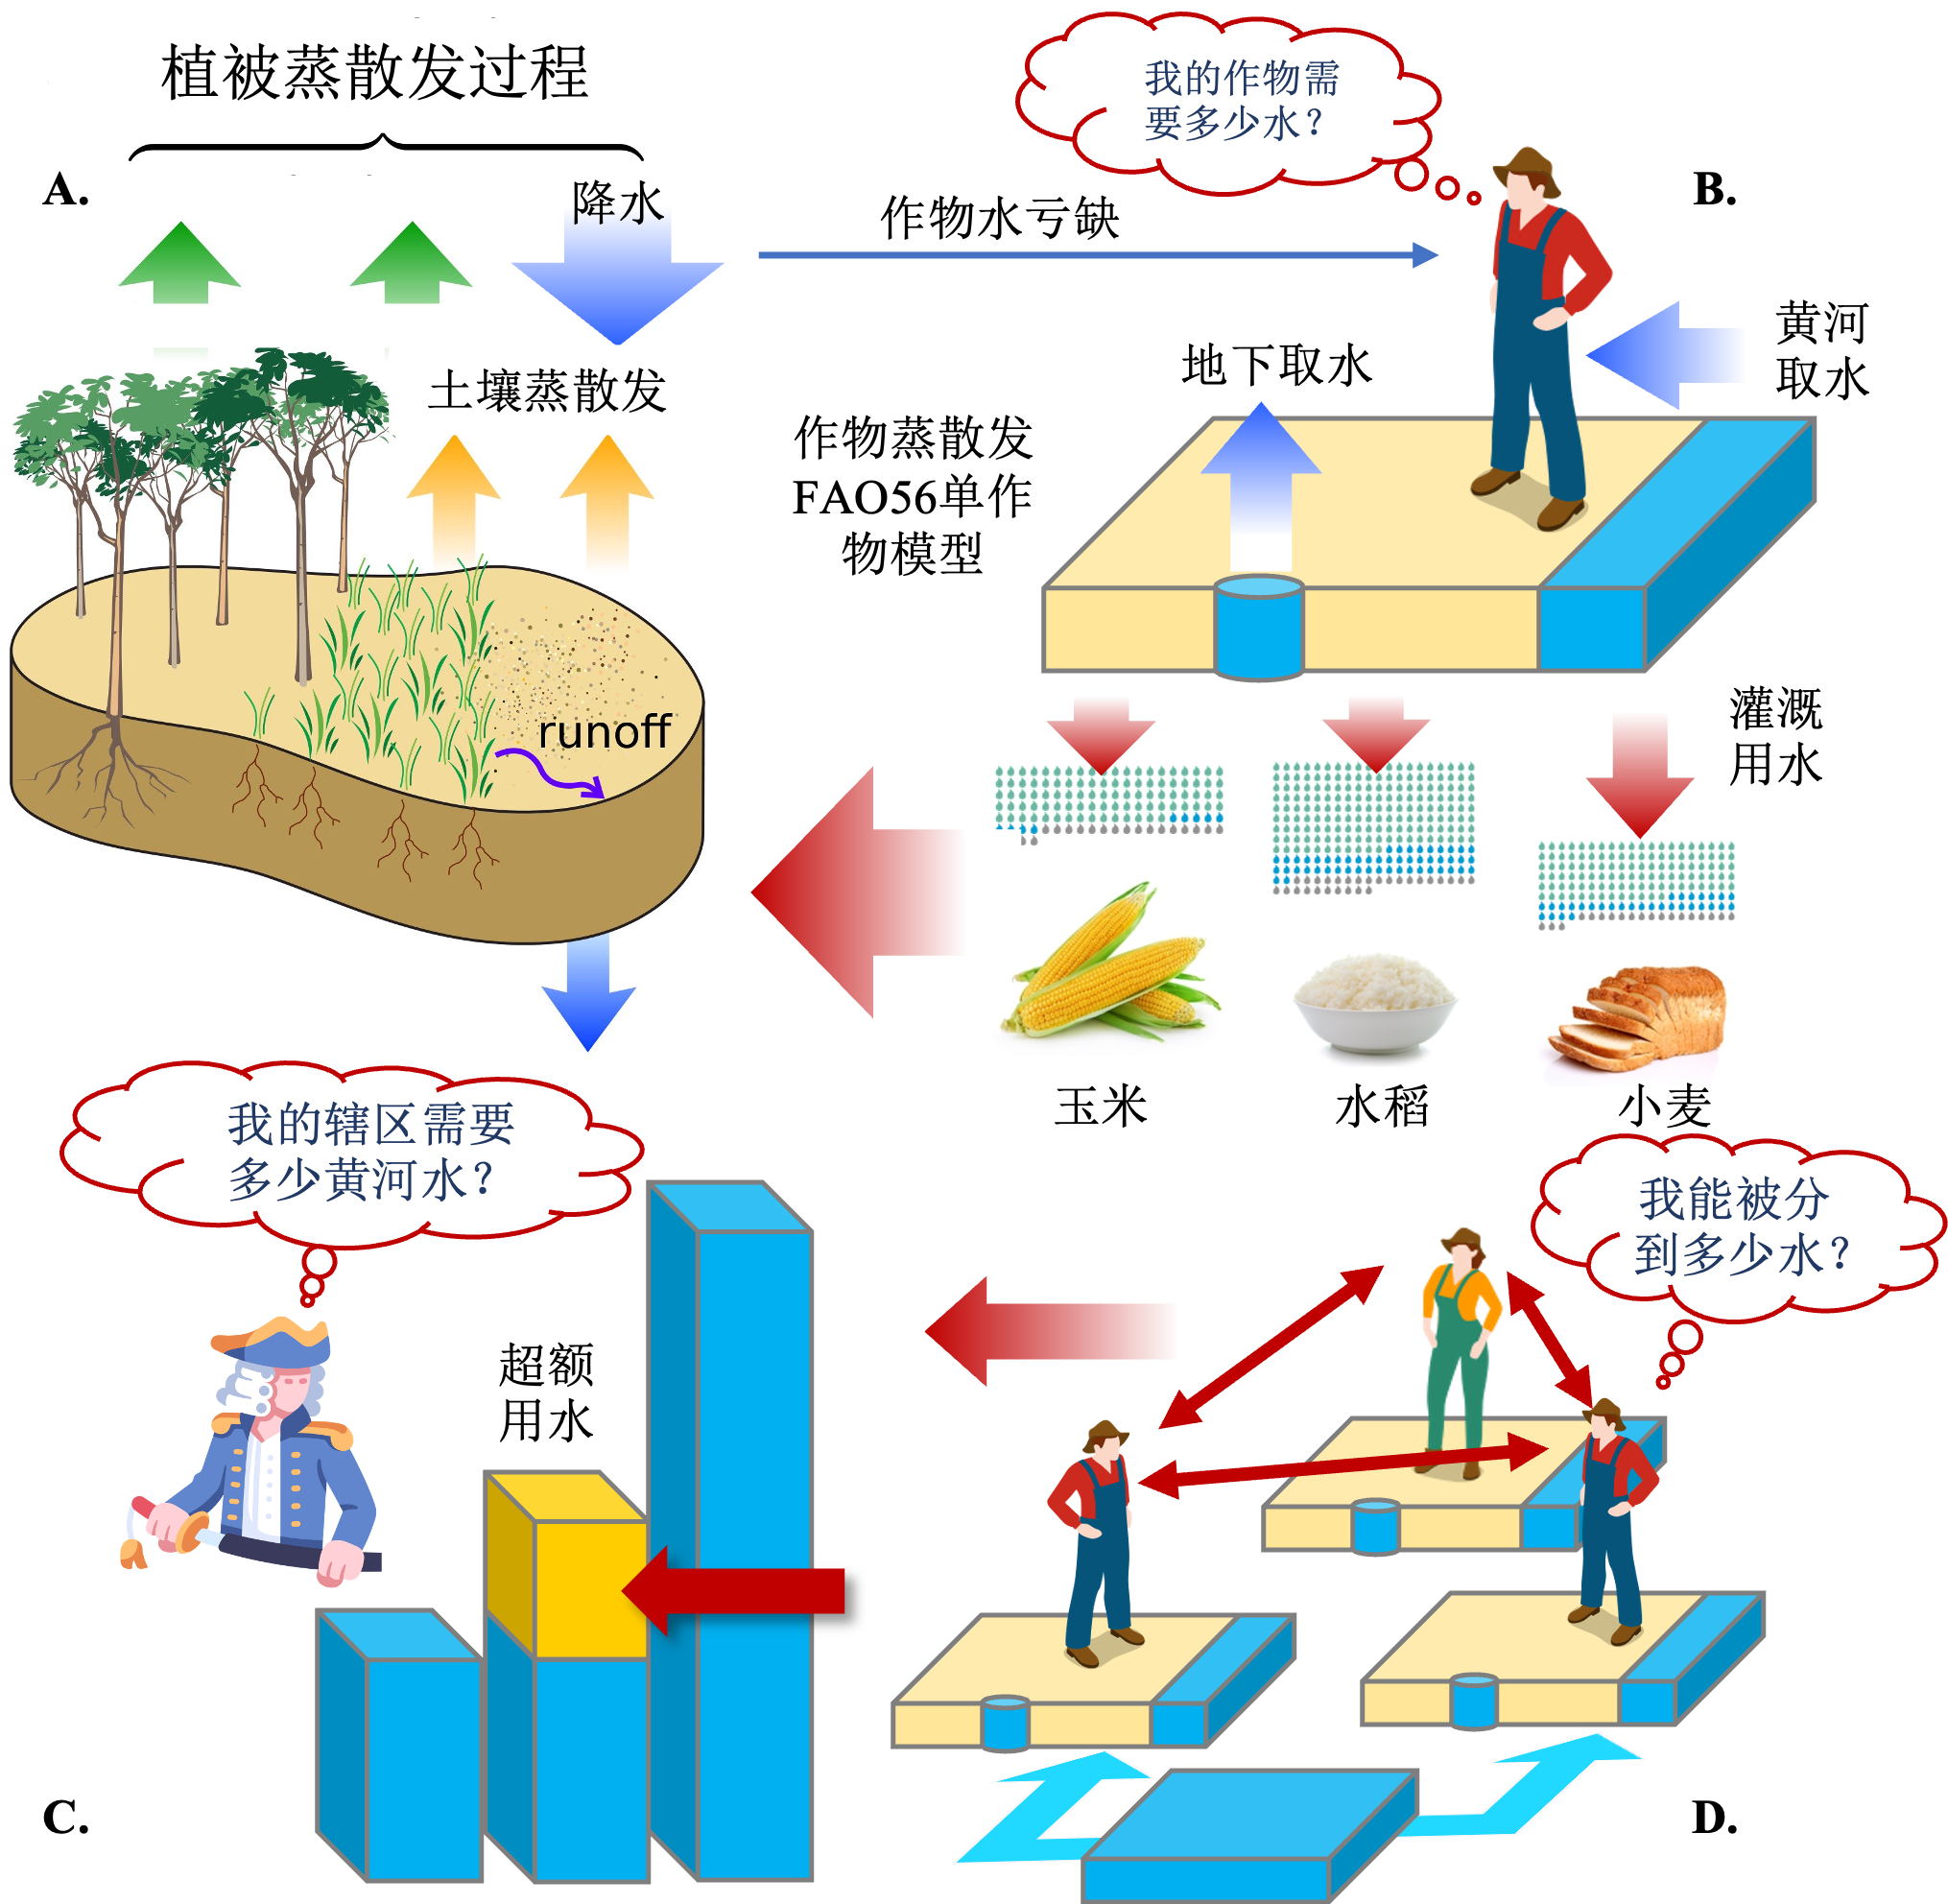
\includegraphics[width=0.8\textwidth]{img/ch6/ch6_framework.png}
    \caption[多主体模型的设计框架]{多主体模型的设计框架。
        \textbf{A.} 自然模块:水文气候条件、流域主体的作物选择和灌溉策略如何影响作物蒸散发。
        \textbf{B.} 人类模块(个体尺度):流域内的灌溉主体在给定水文气候条件、给定配额上限/下限的情况下如何决定其用水来源及用水量;
        \textbf{C.} 地区尺度:体现制度变化对区域总可用水配额的影响。
        \textbf{D.} 流域尺度:体现流域系统的主体分布、主体网络结构特征对主体博弈决策的影响。
    }\label{ch6:fig:framework}
\end{figure}

\subsubsection{个体尺度}

对单个灌溉主体而言,灌溉引水决策的核心是对作物在天然降水之外的水亏缺进行人为补给。
水亏缺是考虑灌溉损失后的作物蒸散发与实际降水量之间的差,作物蒸散发则采用国际粮农组织(FAO)推荐的单作物系数法进行计算,由潜在蒸散发和作物蒸散发系数计算得到。

\begin{equation}
    \label{ch6:eq:deficits}
    W_{deficits} = \frac{ET_c - P}{k_{loss}}
\end{equation}

\begin{equation}
    \label{ch6:eq:etc}
    ET_c = ET_{0} * Kc
\end{equation}

其中潜在蒸散发和降水根据主体所处的位置直接从自然模块调用相应属性,作物蒸散发系数$Kc$的同样通过查阅采用国际粮农组织($FAO56$)推荐的作物表得到(表\ref{ch6:tab:crops})。


% Table generated by Excel2LaTeX from sheet '作物物候表'
\begin{table}[htbp]
    % \centering
    \caption[黄河流域三种主要粮食作物的物候表]{黄河流域三种主要粮食作物的物候表$^a$}
      \begin{tabularx}{\textwidth}{p{0.8cm} LLLLL p{0.8cm} p{0.8cm} p{0.8cm}}
      \toprule
      作物  & \multicolumn{1}{l}{播种期} & \multicolumn{1}{l}{萌发期} & \multicolumn{1}{l}{生长期} & \multicolumn{1}{l}{中期} & \multicolumn{1}{l}{后期} & \multicolumn{1}{l}{$Kc_{ini}$} & \multicolumn{1}{l}{$Kc_{mid}$} & \multicolumn{1}{l}{$Kc_{end}$} \\
      \midrule
      小麦    & 4月5日  & 4月25日 & 5月20日 & 7月19日 & 8月18日 & 0.15  & 1.15  & 0.30  \\
      水稻    & 4月15日 & 5月15日 & 6月14日 & 7月14日 & 8月13日 & 1.00  & 1.20  & 0.70  \\
      玉米    & 4月19日 & 5月9日  & 6月13日 & 7月23日 & 8月22日 & 0.15  & 1.20  & 0.50  \\
      \bottomrule
    \end{tabularx}\label{ch6:tab:crops}%
    \footnotesize\\
    $a$ 本模型不考虑冬小麦的种植。
\end{table}%


但在农民生产实际中,基本不可能做到完全按照作物的水亏缺决定灌溉量,而是根据经验,既往文献中通常在水亏缺基础上额外使用一个系数$\alpha$表示实际决策中的灌溉量,该系数估计了农民对作物水亏缺的经验认知与节水灌溉的影响,即实际灌溉用水量$WU$可表示为:

\begin{equation}
    \label{ch6:eq:WU}
    WU = W_{deficits} * \alpha
\end{equation}

但在本章研究中,由于时间跨度较长($1980 \sim 2010$),区域灌溉的节水升级改造是响应制度变化的重要措施,系数$\alpha$一定是剧烈变化的。
因此,本章研究根据用水量$WU$的年际统计数据将尺度下降到月尺度,$WU_i$代表农民在作物生长季在第$i$个月的实际的用水需求,而经验系数$\alpha$的值则可以作为反映灌溉节水的指标,则有:

\begin{equation}
    \label{ch6:eq:WUi}
    WU_i = WU * \frac{W_{deficits, i}}{\sum_{i} W_{deficits, i}}
\end{equation}

其中$i$为模型的每个时间步长单位(月),因此在每步模拟中,可将每个灌溉主体的作物生长用水来源$W$分为降水来源$W_p$、地表水来源$W_s$、地下水来源$W_g$三部分,具体用水决策及模型计算顺序如下:
(1)根据降水和作物蒸散感知水亏缺$W_{deficits}$,如果$W_{deficits}=0$,说明降水已经满足了需求,则作物生长水源$W$就完全由降水提供,$W=W_{p}$;
(2)如果降水无法满足作物生长需求,就根据公式\ref{ch6:eq:WUi}评估当月的水需求$WU$,并设定降水来源$W_{p} = P$;
(3)对于需求$WU > 0$,假定农民首先考虑从地表水获得,根据自己的官方配额$Q_{0}$和超采的配额$Q_{1}$决定多取用多少配额$Q = Q_{0} + Q_{1}$,若$Q > WU$,则地表水使用$W_s = WU$,否则$W_s = Q$;
(4)最后估计地表水开采量$W_g$,所有降水和地表水仍不被满足的用水需求都被认为从地下水获取,即$W_g = WU - W_s - W_p$。

\subsubsection{地区尺度}

黄河流域的配额制度通常仅细致到地级市范围,如何在地区尺度分配该地区的可供分配的水资源配额取决于主体之间的自组织。
本章研究中假设地区尺度完全根据作物的水亏缺$WU_{deficits}$分配灌溉水量,作为完全的“按需分配”,这是节约配额的理论最优(也是理论最公平的)情景,这也意味着现实中的资源供需匹配不会比本章研究的模拟结果更好。
在数学上,假设总地表水配额为$Q_{C}$的地区$C$中包含$n$个主体,则主体$j$的配额$Q_j$为:

\begin{equation}
    \label{ch6:eq:quota}
    Q_j = Q_{C} * \frac{W_{deficits, j}}{\sum_{j \in C} W_{deficits, j}}
\end{equation}

由于第五章中介绍的分水制度差异及其变化,地区$C$的配额并非固定不变的,在$1987 \sim 1998$年间水资源配额存在可浮动的特性,使用$Q_{\min}$和$Q_{\max}$两个属性进行表达,允许用水个体的实际地表取用水在其间浮动。
$Q_{\max}$由黄河流域各省在$1983$年自主上报的水资源配额需求基础上降尺度到地区和月份来估算(详见表\ref{ch5:tab:quota}),代表自主取水时期满足该地区主体用水需求的能力上限,通常这是官方建议配额$Q_{\min}$的近两倍。
因此,关于$Q_j$的判定规则如公式\ref{ch6:eq:which_quota}所示,与模型当前模拟的年份$yr$有关:

\begin{equation}
    \label{ch6:eq:which_quota}
    Q_j =
    \begin{cases}
        Q_{\max} & \text{when } yr < 1987 \\
        Q_{\in} \leq Q_j \leq Q_{\max} & \text{when } 1987 \leq yr \leq 1998 \\
        Q_{\min} & \text{when } yr > 1998
    \end{cases}
\end{equation}

在$1987 \leq yr \leq 1998$时期,每个主体在计算配额$Q$时如果有较大的用水需求,其$Q_{0} = Q_{\min}$会保证被优先满足,因为这是分水方案中明确保证的合法配额。
由于这个配额没有被强制执行,该主体拥有一定的灵活性索取获得超越官方建议配额$Q_{\min}$的额外配额$Q_{1}$,即超出制度规定但不违背需求上限的“违背制度”部分,该部分配额的值与主体的社会属性有关,详见\ref{ch6:sec:society}\refname{ch6:sec:society}模块的介绍。
但$Q = Q_{0} + Q_{1}$不会超过该主体能被分配到的最大合理配额$Q_{\max}$。

\subsubsection{流域尺度}

在流域尺度,需要决定主体生成的数量、位置、以及相互作用网络。
气候、水文、人口的空间数据精度同化至$0.1$度,即每个空间栅格的范围大约为$A_{cell} = 121{km}^2$,这也是主体进行灌溉活动的基本单元。
本章研究的时间精度是月,考虑作物的生长季主要在$4$月到$8$月之间(见表\ref{ch6:tab:crops}),因此根据统计数据中三类主要作物的灌溉面积和模拟的空间精度来估计每个地级市的主体数量。

\begin{equation}
    n_{C} = \sum_{k=R, M, W}\frac{A_{C, k}}{A_{cell}}
\end{equation}

其中$k = R, M, W$分别代表本研究考虑的三种作物:水稻、玉米和小麦,$A_{C, k}$为该种作物在$C$市的灌溉面积,$A_{cell}$则为每个斑块(栅格)代表的面积。
由于各地级市的面积每年都会变化,主体数量也会每年使用新的统计数据来进行更新。
每个栅格只能同时存在一个主体,在保证主体数量与灌溉面积一致的基础上,主体生成的位置是随机的,概率遵循以人口空间分布的加权平均。

主体决策之间会互相影响,每年的主体数量和位置更新后,还需要预设主体之间的交互关系。
以每个主体为一个节点,存在相互影响的主体间存在连边,那么整个流域可形成一个复杂网络,该网络可包括三种潜在连边:
(1)同一地级市的灌溉主体之间
(2)不同地级市的灌溉主体之间
(3)不同省区的灌溉主体间
由于中国农业基本单元的封闭性,本研究假设不同省之间的主体之间不会互相影响(即不会出现跨省互相影响决策的情况),在同一地级市之内和地级市之间的连边遵循具有固定连边概率的ER随机图(Erdős–Rényi random graphs)构建算法(Erdos and Renyi, 1959),即随机图是一个由$C * n$个节点组成的图,其中同一地级市每对节点连接的概率为$p_n$,不同地级市之间则每对节点的连接概率为$p_C$。
因此一旦概率对$p_n$,$p_C$给定,全流域范围内所有灌溉主体之间可能互相影响的网络拓扑关系就被确定了。

\subsection{模块构建与耦合}

在上述规则构架下,本研究包括两个关键模块:
(1)人类模块:流域内的灌溉主体在给定水文气候条件、给定配额上限/下限的情况下如何决定其用水来源及用水量;
(2)自然模块:水文气候条件、流域主体的作物选择和灌溉策略如何影响作物蒸散发。
本节先分别介绍两个模块的运行过程,最后介绍二者间的耦合反馈关系。

\subsubsection{人类模块}\label{ch6:sec:society}

在人类模块中,本研究使用演化公共池塘博弈的分析框架对主体面对配额限制的决策响应进行分析,使用遵循配额($C$)与违背配额($D$)来概括主体在面对灵活水配额制度($1987$年至$1998$年间)的基本决策。
博弈论(Game Theory)是研究决策者之间战略互动的数学模型,是研究具有竞争性质现象的理论和方法,对于公共水配额这种竞争性、排他性都很强的的“公共池塘资源”,符合演化公共物品博弈的模型框架\cite{ostrom2009, traulsen2010}。
演化公共池塘博弈框架又称多代理人囚徒困境博弈,本研究中主体$i$选择是否遵循限制地表用水的配额制度($S_i = 1$表示合作$C$,$S_i=0$代表决策$D$)。
如果某个主体同意严格遵循配额制度$Q = Q_{\min}$,那么他将损失潜在收益$c$中的一部分。
如果每个人都遵循配额(选择合作$C$),那么共同投资的总额可能会变成原来的$r$倍,并在所有参与的投资者中平分。
如果有$N$个代理人参与,那么每个人的博弈收入$E$如由两部分组成(见公式\ref{ch6:eq:game}):$-c*S_i$ 代表单个主体对集体贡献的成本,而 $\sum_{j=1}^N S_j$则代表共同利益池给每个贡献的主体分到的利益。

\begin{equation}
    \label{ch6:eq:game}
    E=-c * S_i+\frac{r c}{N} \sum_{j=1}^N S_j=-\left(c-\frac{r}{N}\right) S_i+\frac{r c}{N} \sum_{j \neq 1}^N S_j
\end{equation}

在本研究中,黄河分水制度对于遵循配额的主体没有任何额外的经济补贴(这被视为一种行政上的义务行为),也没有正式的经济上的行政处罚,因此公共池塘的收益系数$r = 1$。
此外,因为黄河流域灌区的地下水取水的成本普遍高于地表取水,潜在成本$c$与地下水开采量$W_g$有关,使用$c \propto W_g = k_e * W_g$表示,本研究中为直观考虑采取经济系数$k_e = 0.3$,即意味着地下水水费每单位比贵$0.3$单位。
这个系数的取值实际上不会影响模型表现,因为本研究后续影响主体决策的是主体间的收入差距,而所有主体的潜在收益$E$与地下水取水量都是同样的线性关系,决定主体收益差距仅由地下水开采量$W_g$的差距决定。
因此理论上可预期的是,在响应制度的经济驱动因素上,遵循配额会产生大量地下水开采成本的地区将拥有更大的动机违背配额。

作为没有任何补贴的制度,影响主体是否遵循配额的另一个主要驱动因素是社会规范,因为即便没有经济惩罚,违背制度也是不被提倡的。
多元理性理论是一个理解个人决策与社会规范影响之间关系的经典框架,指出由“个体/集体主义”与“注重/轻视规范”两个维度,就可以预测不同文化背景下遵循社会规范的倾向\cite{verweij2015},因此可以对复杂的政策问题进行结构化的诊断,因此该方法框架已被应用于解释水治理的成功与失败。
参考 Castilla-Rho 等人基于多元理性(Plural rationality theory PRA)的社会理论的一系列研究,可以使用两个简单的参数$b$和$v$来测量主体遵循制度规范的动因。
其中$b\in[0, 1]$表征某主体“注重/轻视规范”的程度,在模型中也是该主体突破规定配额,做出决策$D$的概率。
$v \in [0, 1]$则表征主体“个体/集体主义”的程度,该参数越大代表主体越重视与他人保持一致,在模型中是对该主体社交网络中违规行为进行负面评判的概率。
考虑到人们不愿意主动得罪别人,也不愿意丧失名誉,这种评价将成为计算社会得分的基础,采用在福利经济学中常用的Cobb-Douglas函数的形式进行表达:
% Cobb-Douglas函数(https://inomics.com/terms/cobb-douglas-production-function-1456726)
% [Happy Planet Index](https://happyplanetindex.org/) 
% 人类发展指数(http://hdr.undp.org/en)
\begin{equation}
    S = {(grid)}^m * {(1 - group)}^n
    \label{ch6:eq:society}
\end{equation}

其中 $m$ 是一个主体发现其它人违规超配额用水的次数,$n$ 则是他被他人发现超配额用水的次数。
即$grid^m$ 这部分表达的是主体因周围人违背制度规范而感到不舒服;$group^n$ 这部分表达的是一个主体违背制度规范而被周围人指指点点而感到不舒服。
$grid$与$group$是反映社会整体平均$b$与$v$水平的参数。

在演化博弈中,决策还是可演化的(Evolutionary),因为一些反应因为符合社会规范而受到奖励,而另一些反应则因为背离社会规范而受到惩罚。
人类模块在每一个时间步的最后将计算所有主体的博弈结果——$0 \sim 1$标准化后的经济得分($E$)与社会得分($S$),并将两者平均$Score = E * S$作为主体的最终得分。
在社会网络中,表现最成功的主体决策以一定概率$p_{l}$被他的朋友们学习,学习后的主体使用被学习对象的$b$和$v$参数代替学习者原本的参数。

综上所述,在人类模块的每次模拟中,每个主体都将遵循图\ref{ch6:fig:society}所示的流程图:

\begin{figure}[htb]
    \centering
    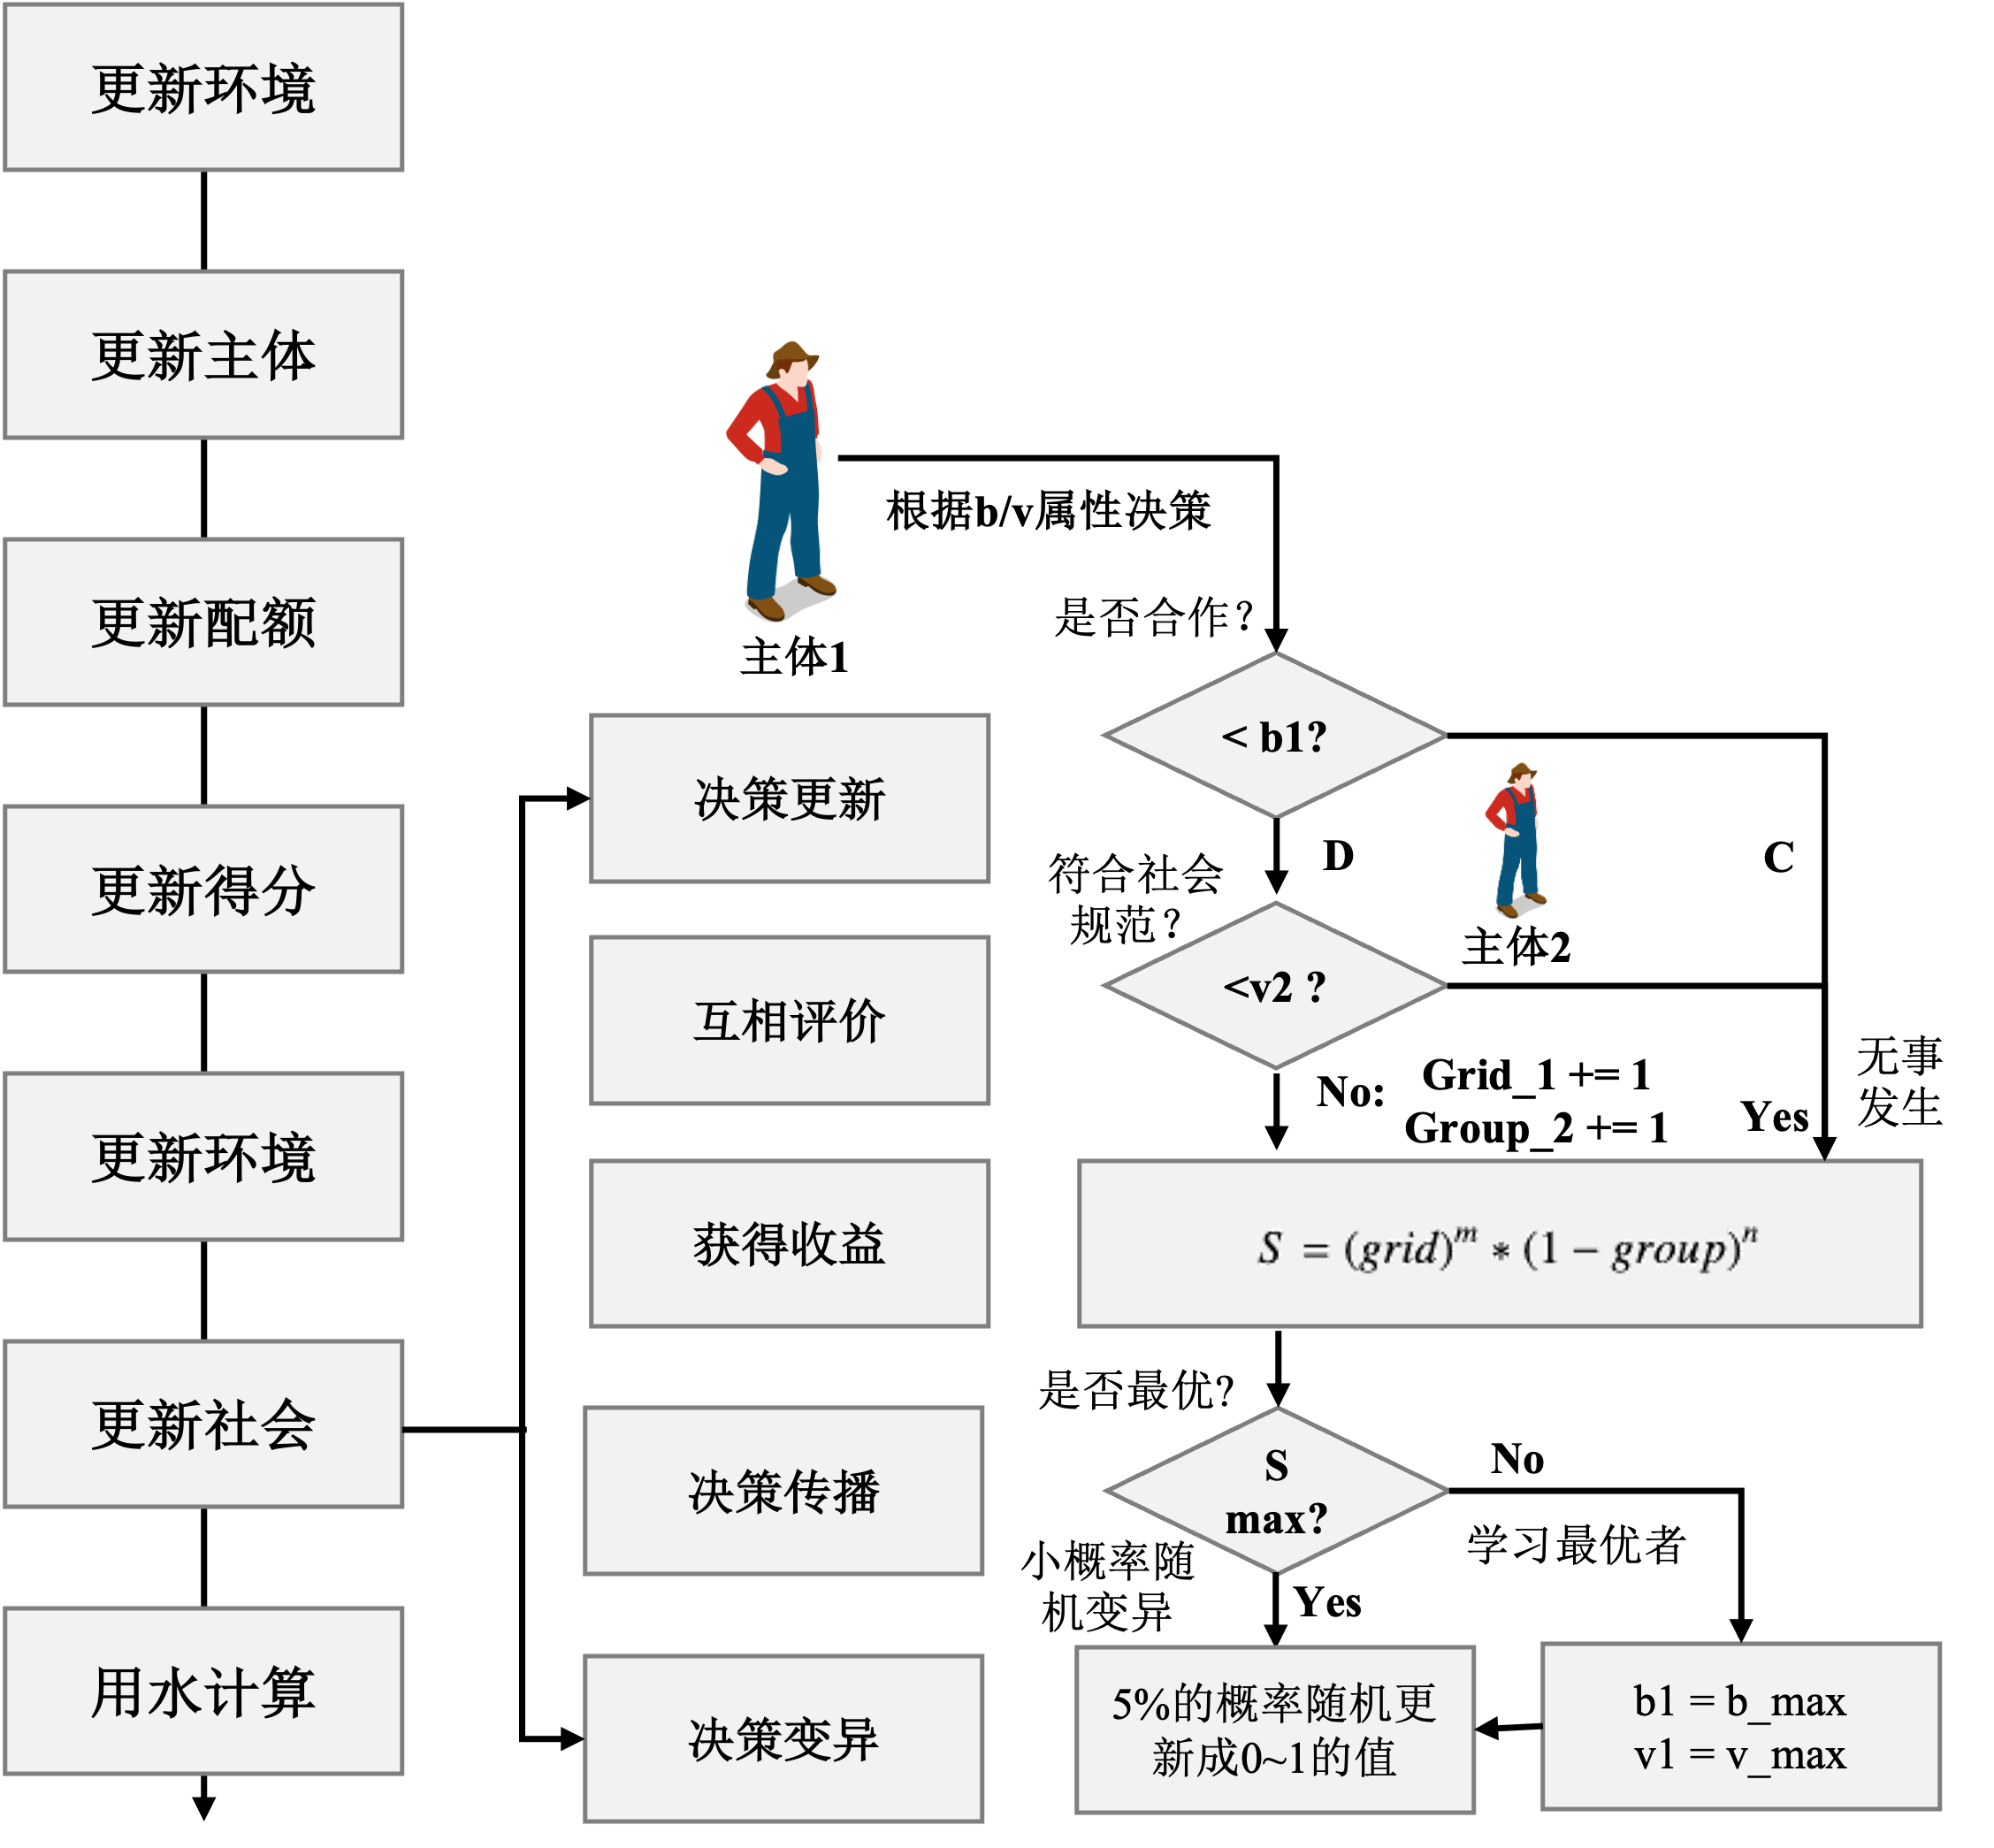
\includegraphics[width=0.8\textwidth]{img/ch6/ch6_updates_diagram.png}
    \caption[多主体模型的更新规则与模拟流程]{多主体模型的更新规则与模拟流程。
    左侧表示多主体模型整体运行的大致流程,“更新社会”步骤是人类模块进行决策的部分,包括五个主要步骤:
        (1)主体根据自己当前的$b$属性(“注重/轻视规范”)作为选择合作的概率,决定本轮中使用的决策“C/D”。
        (2)若当前主体选择不合作(D),其余选择合作(C)的主体根据其$v$属性(“个体/集体主义”)决定是否对其进行社会规范上的谴责。
        (3)对每个主体按照谴责他人/被他人谴责的次数估计自己的社会收益$S$。
        (4)综合社会收益$S$和经济收益$E$,每个主体都将学习自己朋友中综合表现最好的个体,模仿他的$v$和$b$属性,若自己的表现就是朋友中最好的,则跳过此步骤。
        (5)为避免模型陷入局部最优,以极小概率($\alpha = 5\%$)对主体的策略进行变异,设置$v, b \in [0, 1]$成新的随机数。
    }\label{ch6:fig:society}
\end{figure}

\subsubsection{自然模块}

在自然模块中,本研究使用 FAO56 推荐的算法计算潜在蒸散发$ET_0$、作物蒸散系数$Kc$、以及作物蒸散发$ET_c$:

\begin{equation}
    ET_c = ET_0 * Kc * Ks
\end{equation}

其中$Ks$是水应力系数,主要与土壤质地有关。由于在本研究中仅考虑三种主要粮食作物,且主要分布在灌溉条件良好的土壤上,对此系数的空间分异不再作进一步考虑,使用系数$Ks = 0.3$进行估计。  % TODO chen 2023

潜在蒸散发$ET_0$的计算方法使用Penman-Monteith方法,式\ref{ch6:eq:pm}:

\begin{equation}
    \label{ch6:eq:pm}
    PET = \frac{0.408 \Delta (R_{n}-G)+\gamma \frac{900}{T+273}
    (e_s-e_a) u_2}{\Delta+\gamma(1+0.34 u_2)}
\end{equation}

其中$Rn$为作物表面上的净辐射,$MJ/(m^2 day)$;$G$为土壤热通量,$MJ/(m^2 day)$;$T$为$2$米高处日平均气温$^\circ C$;$u2$为$2$米高处的风速,$m/s$;$es$为饱合水汽压,$kPa$;$ea$为实际水汽压$kPa$;$es - ea$为饱和水汽压差,$kPa$;为饱和水汽压曲线的斜率;$r$为湿度计常数,$kPa/^\circ C$。
由于计算的时间尺度(月),土壤热通量可以忽略。根据其它数据可得性,对经验公式\ref{ch6:eq:pm}中的饱和水汽压$es$使用气温数据进行估算:

\begin{equation}
    e^0(T) = 0.6108 * \exp \frac{17.27 T}{T + 237.3}
\end{equation}

\begin{equation}
    es = \frac{e^0(T_{\max}) + e^0(T_{\min})}{2}
\end{equation}

作物生长期间的作物系数$Kc$的曲线是用三个阶段的作物系数来估计的:初期($Kc_{ini}$)、中期($Kc_{mid}$)和后期($Kc_{end}$)。
作物系数的各转折点以表\ref{ch6:tab:crops}中的数据为依据进行定位。
$Kc_{ini}$的计算方法如下\cite{allen1998}。

\begin{equation}
    \label{ch6:eq:kcini}
    K_{\text {c, ini}}=\frac{\mathrm{TEW}-(\mathrm{TEW}-\mathrm{REW}) \exp \left[-\left(\mathrm{t}_w-\mathrm{t}_1\right) E_{so}\left(1+\frac{\mathrm{REW}}{\mathrm{TEW}-\mathrm{REW}}\right)\right]}{\mathrm{t}_w E T_{\mathrm{o}}}
\end{equation}

其中,$TEW$为总的可蒸发水量($mm$);$REW$为易蒸发水量($mm$);$tw$为初始时期湿润事件之间的平均时间(天);$t_1$为易蒸发水量干燥完成所需的时间(天);$Eso$为由于低含水层湿润土壤或由于以前干燥时期储存在表层的热量而增加的蒸发潜力($mm/d$)。其中$E_{so} = 1.15 * ET_0$, $t_w = \frac{L_{ini}}{n_w + 0.5}$, $t_1 = REW / E_{so}$。

当$t_1 < t_w$的时候,$K_{\text {c, ini}} = 1.15$,否则使用\ref{ch6:eq:kcini}进行估计,且用来$TEW_{cor}$和$REW_{cor}$替代$TEW$和$REW$。

对于渗透深度$depth < 10mm$的所有土壤质地,有:

\begin{equation}
    TEW_{cor} = 10mm \\
    REW_{cor} = \min(\max(2.5, 6 / ET_0^{0.5}, 7))
\end{equation}

对于渗透深度$depth >= 40mm$的所有土壤质地,有:

\begin{equation}
    TEW_{cor} = \min(15, 7 {(ET_0)}^{0.5}) \\
    REW_{cor} = \min(6, TEW_{cor} - 0.01)
\end{equation}

适用于渗透深度$depth >= 40mm$的中、细土质,有:

\begin{equation}
    TEW_{cor} = \min(28, 13{(ET_0)}^{0.5}) \\
    REW_{cor} = \min(9, TEW_{cor} - 0.01)
\end{equation}

对于$depth \in (10mm, 40mm)$,有:
\begin{equation}
    K_{c ini} = K_{c ini(I<=10mm)} + \frac{I-10}{40-10}[K_{c ini(I>10mm)} - K_{c ini(I<=10mm)}]
\end{equation}

其中,$K_{c ini(I≤10mm)}$是指入渗深度 $depth<=10 mm$的所有土壤质地的$K_{c ini}$值;$K_{c ini(I > 40 mm)}$是指入渗深度$depth>40 mm$的粗或中/细土壤质地的$K_{c ini}$值。

$K_{c mid}$ 可以由下式估计:
\begin{equation}
    K_{c mid} = K_{c mid(Tab)} + [0.04(u_2 - 2) -0.004(RH_{\min} - 45)]{(\frac{h}{3})}^{0.3}
\end{equation}

$K_{c end}$ 可以由下式估计:
\begin{equation}
    K_{c end} = K_{c end(Tab)} + [0.04(u_2 - 2) -0.004(RH_{\min} - 45)]{(\frac{h}{3})}^{0.3}
\end{equation}

其中 $K_{c mid(Tab)}$ 和 $K_{c end(Tab)}$ 均是 FAO 作物表中推荐的估计值(见表\ref{ch6:tab:crops})。
完成各阶段作物系数计算后,参考作物的生长周期,逐日还原出当年的作物系数曲线,并通过按月平均匹配到本研究的尺度。

\subsubsection{人地模块的耦合}

本章研究的模型在基于地理数据的多主体建模框架“ABSESpy”基础上搭建,这是一个多主体建模开源框架软件包。
该框架使用真实的地理空间数据集来构建人工社会生态系统,同时充分考虑人类行为因素。
它支持使用地理空间数据,对具有认知、社会影响和反应等行为的主体进行建模,用户可以专注于分别实现人类行为的逻辑和自然过程的仿真,该框架使得两者之间能够轻松地访问和修改变量值。
该框架可以调度任意数量的自然模块和社会模块,并使它们之间松散耦合。
例如在本章研究中,人类用水模块通过作物种植来改变自然模块的作物地表覆被属性,可以简单地使用一句\textit{alter\_nature}命令来完成;自然模块则通过降水、地表蒸散发的变化来影响人类用水模块中的决策环境,主体可以根据其所在位置调用相关的自然属性。

\subsection{数据处理}

\subsubsection{输入数据}

本章研究使用的数据清单如表表\ref{ch6:tab:dataset}所示,包括气象数据、作物物候数据、灌溉面积和灌溉用水数据、用水配额数据、人口数据等,其中较为重要且需要预处理的主要是来自黄河水利委员会公开的水资源配额数据。
该数据仅在2014年后才公开了逐月精度的数据,但包括了每个月水量相较于多年平均水平相差的百分比(即表\ref{ch6:tab:dataset}中所示的距平)。
因此,本研究首先根据该距平值将逐月的配额推演至多年平均水平,进一步假设该水量分配是按各地区实际需求分配的,利用用水量数据将省尺度的配额降尺度到地级市。
例如,对某个属于$I$省的地级市$i$在月份$j$内的灌溉用水配额$Q_{ij}$估计为:

\begin{equation}
    \label{ch6:eq:quota_data}
    Q_{ij} = Q_{I, j} * \frac{WU_{i, j}}{\sum_{j = 1, 2, \dots, 12} WU_{I}}
\end{equation}

由于此分水水量包括了所有产业、所有类型灌溉耕地,所以通过式\ref{ch6:eq:quota_data}计算所得该分水额度$Q$需要进行进一步按比例作细化处理:

\begin{equation}
    Q_{W, R, M} = W_{W, R, M} / WU_{sum} * Q
\end{equation}

其中$W, R, M$分别是本研究主要关注的小麦、水稻、玉米三种黄河流域主要作物的用水量,$WU_{sum}$为该地区的总用水量,利用两者的比例作为系数对此地区的用水额度作进一步按需分配,作为本研究多主体模型中研究三种作物所使用的额度数据。

% Table generated by Excel2LaTeX from sheet '数据来源表'
\begin{table}[htbp]
    \centering
    \caption{多主体模型的数据源}
      \begin{tabularx}{\textwidth}{LLLLLL}
      \toprule
      数据名称  & 变量    & 使用数据的模块 & 模型使用描述 & 时间精度  & 数据来源 \\
      \midrule
      中国区域地面气象要素驱动数据集 & 气温、风速、气压、降水、辐射 & 自然模块  & 计算潜在蒸散发 & 1979年至今,0.1度分辨率,逐月 & 中国区域地面气象要素驱动数据集 \\
      作物物候数据 & 物候生长期 & 自然模块  & 计算作物蒸散发 & 全中国干旱/半干旱区 & 文献(已接收) \\
      灌溉配额数据 & 灌溉配额及其距平 & 人类模块  & 估算用水配额 & 2014年迄今,逐月 & 黄河水利委员会网站 \\
      黄河流域用水数据 & 灌溉面积、灌溉用水量 & 模型规则  & 估算主体数量 & 1965年至2013年逐年 & 文献\cite{zhou2020} \\
      人口分布数据 & 人口数量  & 模型规则  & 生成主体分布位置的概率 & 仅2010年一期 & WorldPop\cite{worldpop2020} \\
      \bottomrule
      \end{tabularx}%
    \label{ch6:tab:dataset}%
  \end{table}%
  

\subsubsection{参数选取}

下表\ref{ch6:tab:params}总结了模型中使用到的主要参数:

% % Table generated by Excel2LaTeX from sheet '重要参数一览表'
% \begin{table}[htbp]
%     \centering
%     \caption{多主体模型使用的主要参数及其取值}
%       \begin{tabularx}{\textwidth}{p{1.5cm}p{2cm} L p{1.5cm} p{1.5cm}}
%       \toprule
%       参数名  & 所属模块  & 参数描述  & \multicolumn{1}{l}{估计值} & 参考 \\
%       \midrule
%       $grid$  & 人类模块  & 反映社会整体平均“注重/轻视规范”的程度 & $0.3$   & Castilla-Rho 2017\cite{castillarho2017} \\
%       $group$ & 人类模块  & 反映社会整体平均“个体/集体主义”的程度 & $0.6$   & Castilla-Rho 2017\cite{castillarho2017} \\
%       $p_l$  & 人类模块  & 演化公共池塘博弈策略传播的概率,$p_l = 1$意味着主体一定会在决策传播中学习表现最好的个体 & $1$     & Santos 2008\cite{santos2008} \\
%       $Ks$    & 自然模块  & 水压力系数,主要与土壤质地有关 & $0.3$   & Chen 2023 \\
%       $k_{loss}$ & 自然模块  & 灌溉损失系数 & $0.8$   & Chen 2023 \\
%       $p_{n}$  & 模型规则  & 地级市之内主体建立社会关系的概率 & $1$     & Santos 2008\cite{santos2008} \\
%       $p_{C}$  & 模型规则  & 省之间主体建立社会关系的概率 & $1$     & Santos 2008\cite{santos2008} \\
%       \bottomrule
%       \end{tabularx}%
%     \label{ch6:tab:params}%
%   \end{table}%


本研究所有的参数估计都有前人研究作为参考,需要特别说明的参数选取及其意义主要有三部分:
(1)影响人类模块得分计算的两个社会效用函数在过往的研究中已经被多次使用,且基于问卷数据进行了较为可靠的估计,本研究直接参考Castilla-Rho 研究中从世界价值观调查数据库中对这两个参数的估计值\cite{castilla-rho2015, castilla-rho2017, castilla-rho2020}。
(2)自然模块的$Ks$是水应力系数,主要与土壤质地有关。由于在本研究中仅考虑三种主要粮食作物,且主要分布在灌溉条件良好的土壤上,对此系数的空间分异不再作进一步考虑,使用系数$Ks = 0.3$进行估计。灌溉损失系数则是经验值$0.8$,代表无论如何都有$20\%$的水分会在灌溉中损失掉。
(3)人类模块的$p_l$概率、模型规则中的$p_n$、$p_C$参数都与社会网络的形成有关。Francisco 等人的研究已经对网络结构对演化博弈决策行为传播的影响做了很经典的研究,本研究将三个概率参数均设置为$1$则每个省区都将形成典型的“星形网络”,根据其研究结果,这是一种促进决策传播的有效结构,广泛存在且与已有文献之间具备可对比性\cite{santos2008}。
此外,根据罗家德等人的研究,这也较为符合我国地方社会“以能人为核心”的关系网络结构\cite{luojiade2013}。

% \subsubsection{敏感性检验}

\subsubsection{趋势分析方法}

本研究使用广义加性模型(Generalized Additive Models, GAM)分析地区用水量随时间变化的趋势,这是一种广泛应用于回归分析的非参数统计模型。
相比于线性回归模型,GAM 没有对因变量和自变量之间的关系做出先验假设,因此在数据非线性、非正态分布、存在交互作用等情况下更具有优势。
GAM 通过使用光滑的非参数函数(如样条函数)对自变量的影响进行建模,同时也可以应用广义线性模型中的方法来对非正态数据进行回归分析。


\subsubsection{建模和分析工具}

所有模型使用Python软件3.11版本进行构建,使用到的软件包均为开源软件,版本及其用途如表\ref{ch6:tab:packages}所示。
% 本章构建的多主体模型暂时不予以开源,但具体构建方式已在上述方法中进行了详尽描述。

% Table generated by Excel2LaTeX from sheet '使用包一览表'
\begin{table}[htbp]
    \centering
    \caption{多主体模型使用的开源软件包}
      \begin{tabularx}{0.9\textwidth}{p{2cm} p{1.5cm} L}
        \toprule
      名称    & 版本号   & 描述 \\
      \midrule
      ABSESpy & 0.1.3 & 自动建设简单的 ABM 模型 \\
      hydra-core & 1.3.2 & 简化应用程序的配置 \\
      xarray & 2023.2.0 & 处理标记数据数组的 Python 库 \\
      rasterio & 1.3.6 & 用于读写栅格数据的 Python 库 \\
      geopandas & 0.12.2 & 处理地理空间数据的 Python 库 \\
      rioxarray & 0.13.4 & Rasterio + xarray:利用 xarray 的能力读取和处理栅格数据 \\
      networkx & 3.0 & 创建、操作和学习复杂网络的工具 \\
      dataclasses-json & 0.5.7 & 将数据类编码为 JSON 的 Python 库 \\
      China-Water-Uses & 0.1.0 & 加载、组织和绘制中国用水数据 \\
      fiona & 1.9.1 & 读写 GIS 数据格式的 Python 库 \\
      seaborn & 0.12.2 & 用于绘制漂亮且有信息量的统计图形的 Python 库 \\
      geocube & 0.4.0 & 将栅格数据转换为向量数据的 Python 库 \\
      pygam & 0.8.0 & Python 的 GAM 工具 \\
      \bottomrule
      \end{tabularx}%
    \label{ch6:tab:packages}%
  \end{table}%
  


% \section{主要结果}\label{ch6:results}
\section{灌溉需求与分水配额的失配}

\begin{figure}[!ht]
    \centering
    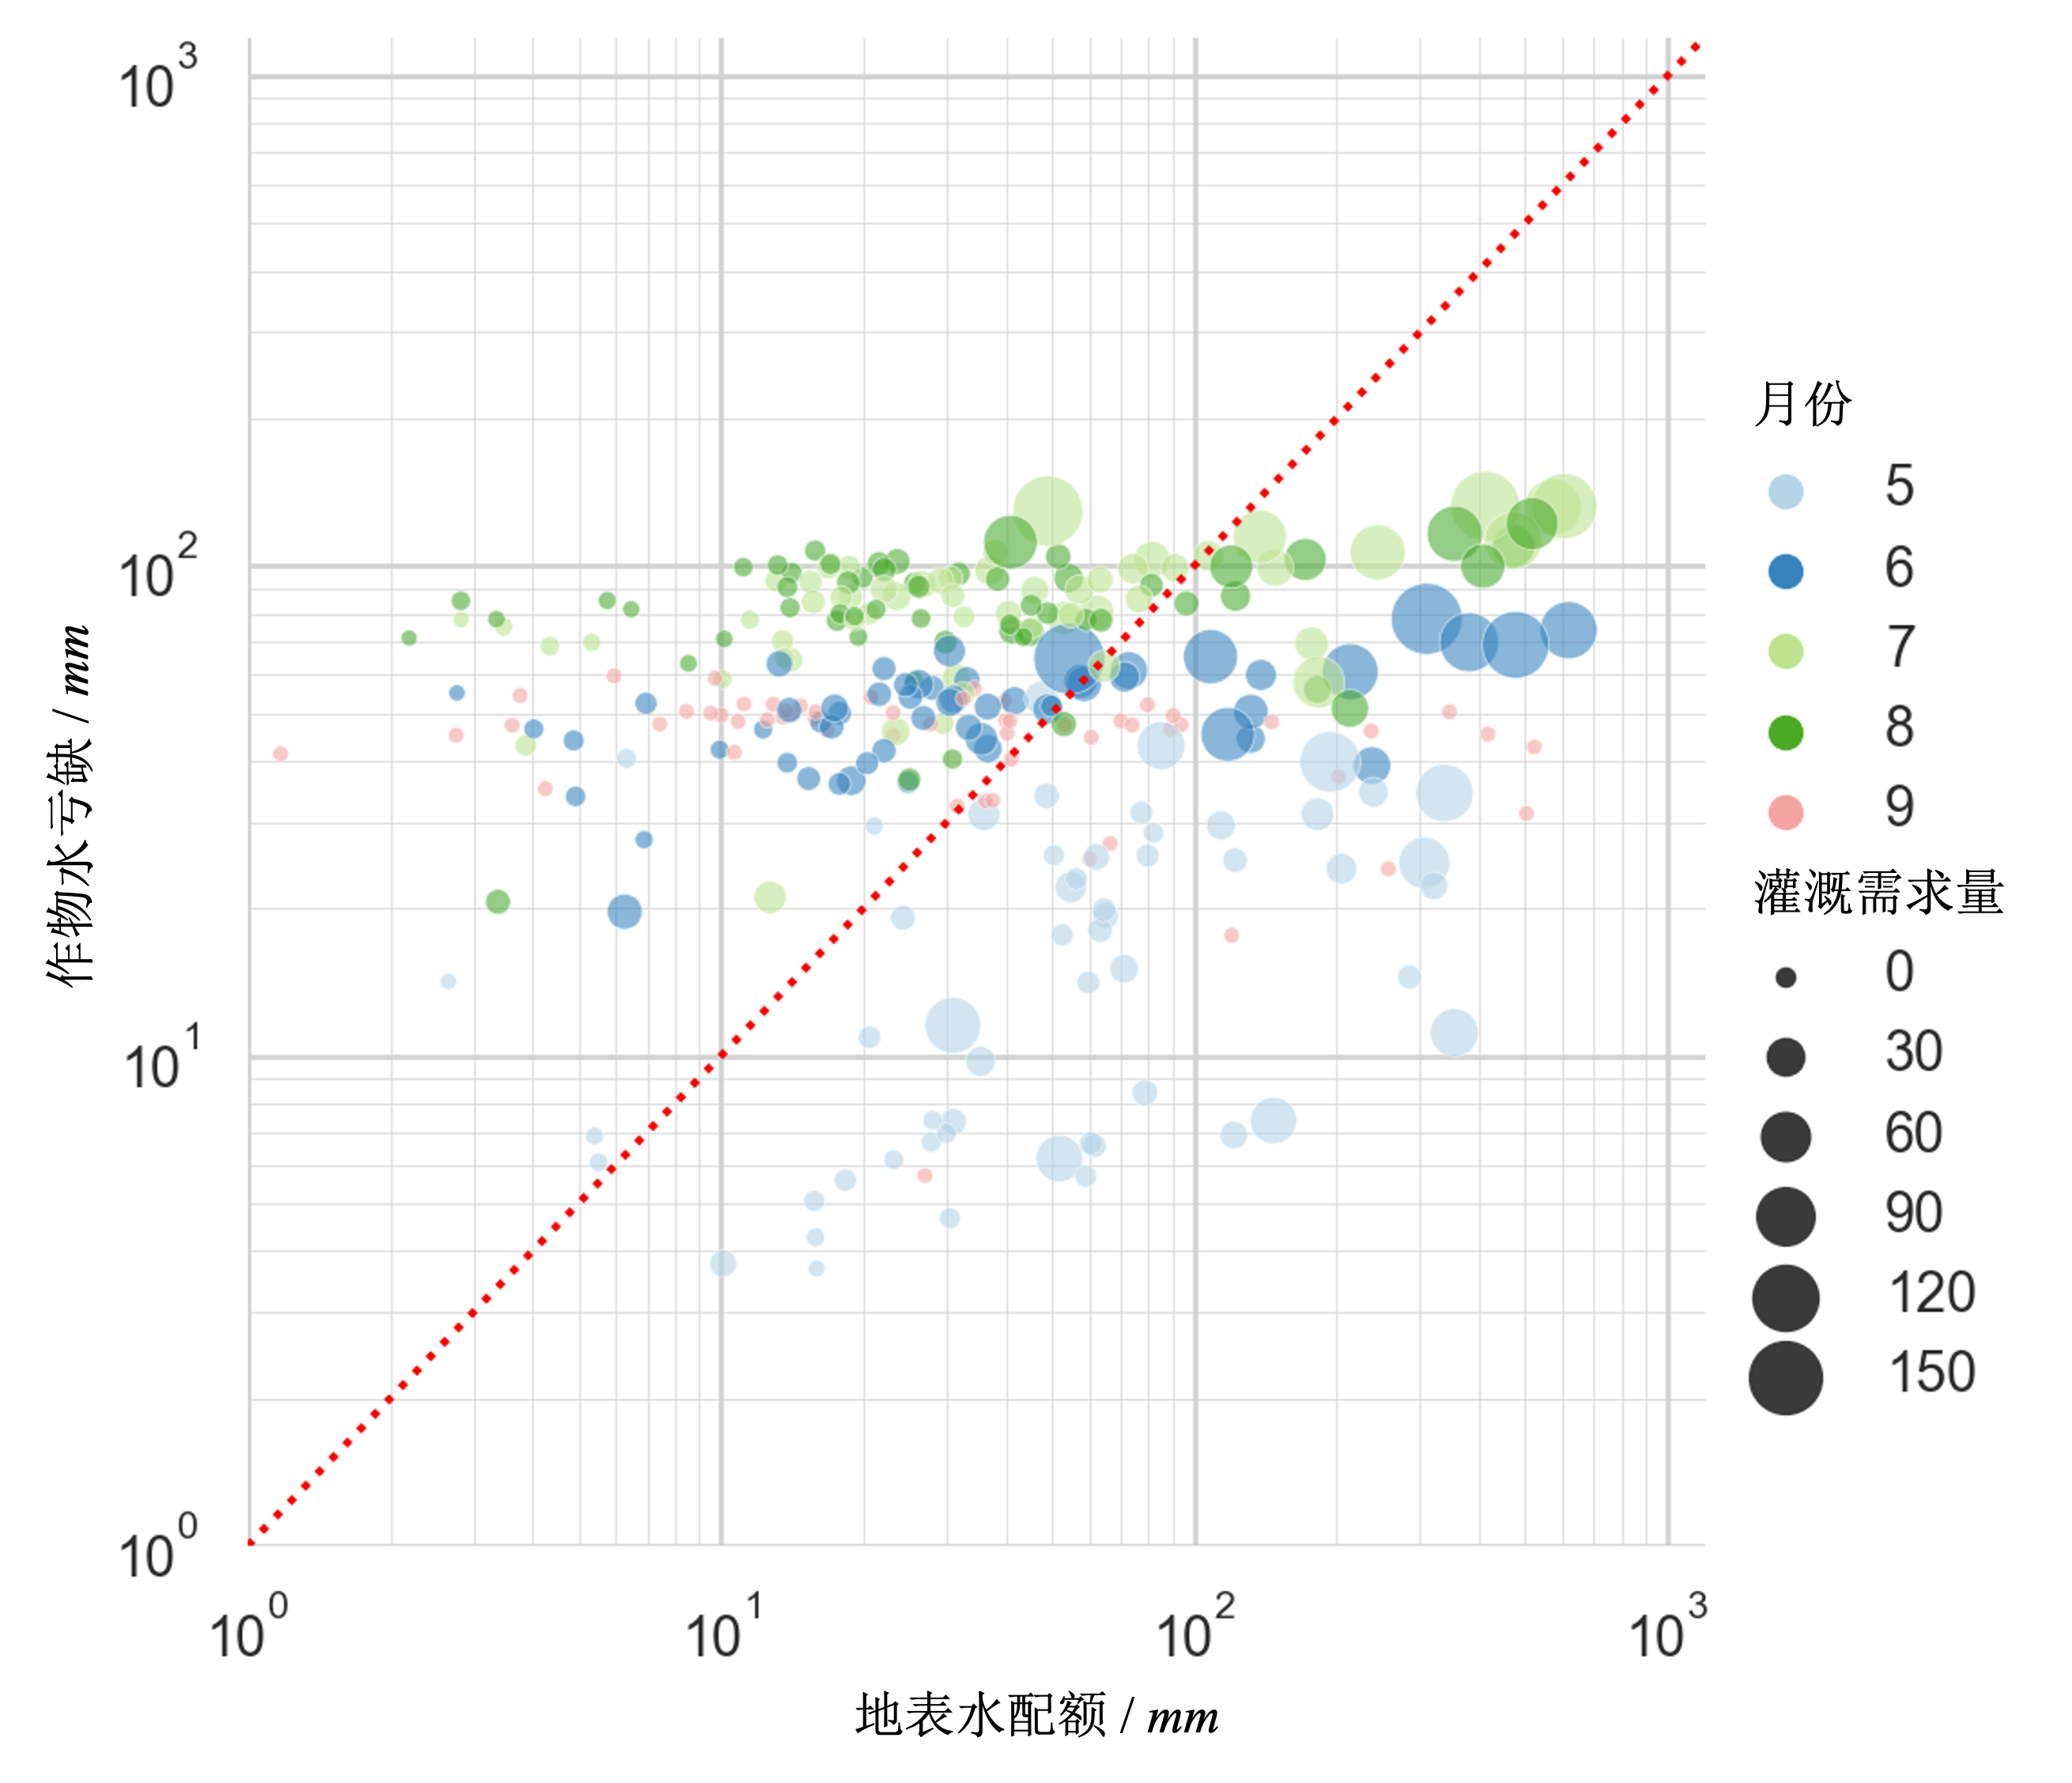
\includegraphics[width=0.8\textwidth]{img/ch6/ch6_matches.png}
    \caption{黄河流域各地级市主要粮食作物生长季水亏缺与地表水配额}\label{ch6:fig:matches}
\end{figure}

图\ref{ch6:fig:matches}展示了月尺度水资源配额与作物水资源亏缺的关系。
红色虚线表示两者的$1:1$线,右侧表示配额大于作物需求,左侧则表示配额小于作物的绝对用水需求。
可见黄河地表水配额与作物水亏缺存在时空分布不匹配现象,因为如果两者匹配得很好,大多数气泡点应该落在$1:1$线上。
气泡的大小代表了统计数据中的地区实际总灌溉用水量,可见水需求量较大的大型灌区也获得了较多的用水配额,容易出现配额供给大于实际作物需求的情况,而在规模偏小的地区则存在水配额供小于求的情况。
此外,气泡的颜色代表了作物生长季的不同月份,可见$6$月到$9$月之间的水资源供需失配情况分布比较相似,都是高需水地区有富余,低需水地区存在不足;仅在作物生长的初期($5$月)的配额普遍出现水资源配额富余的情况。

\begin{figure}[!ht]
    \centering
    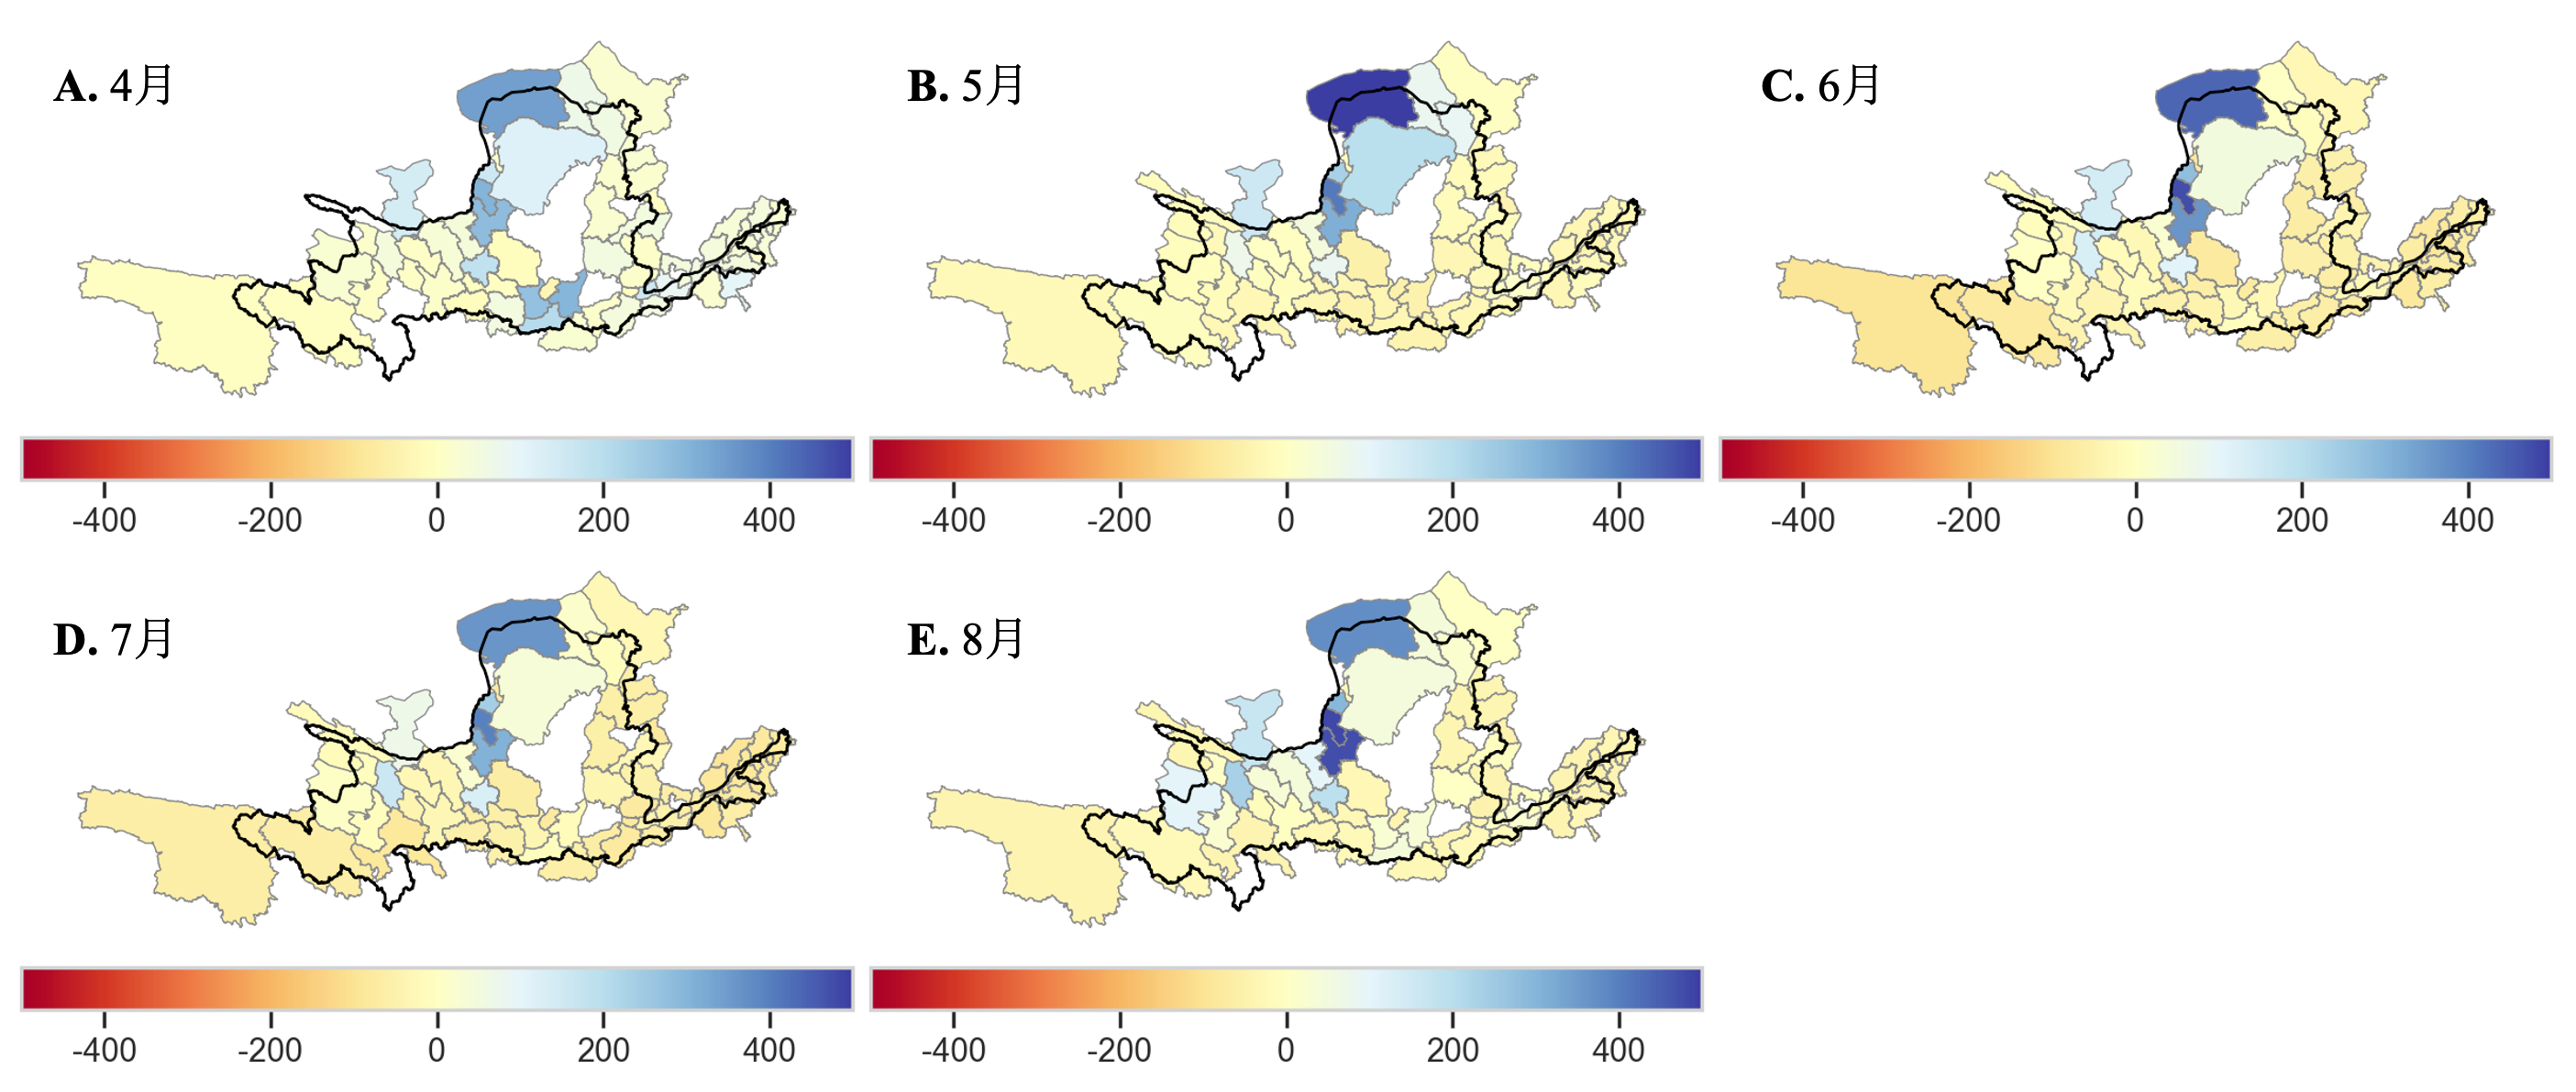
\includegraphics[width=\textwidth]{img/ch6/ch6_deficits_map.png}
    \caption[黄河地表水配额与主要粮食作物需水量之差]{黄河地表水配额与主要粮食作物需水量之差(单位$mm$),$A \textendash{} E$分别表示4月至8月的情况。}\label{ch6:fig:deficits_maps}
\end{figure}

进一步将尺度水资源配额与作物水资源亏缺的差值映射到地图上(图\ref{ch6:fig:deficits_maps}),可以发现大多数地区五月的配额仍属于供需平衡的状态,但河套灌区已经有非常明显的配额富余。
而六、七月的供需失配情况更加严重,不仅河套灌区作物需求和配额供给之间的差异部分地区有超过$500~mm$的配额富余,黄河流域的其它地区则平均有$100~mm$左右的配额亏缺,尤其是下游河南、山东的灌区,均有严重的配额不足情况。

% \section{用水者对分水制度变化的响应}

% 本研究根据每年的灌溉面积确定主体数量,水稻、玉米、小麦各类粮食作物灌溉主体的数量分布如图\ref{ch6:fig:agents}所示,其中小麦种植面积最广,玉米其次,水稻仅部分地区有少量分布,地级市尺度上平均生成的主体数量不足$2$个。
% 将1987年“八七”分水方案出台后的每三年分成一个时间段,将此地表水配额灵活时期分为初期($1988 \textendash{} 1991$)、中期($1992 \textendash{} 1994$)、后期($1995 \textendash{} 1998$)三个时段,诸省份农业主体在不同时期对水资源配额的合作比例如图\ref{ch6:fig:compliacne}所示。
% 可见,由于社会系统存在决策的演化传播,违背分水制度进行超额取水的主体比例会随时间变化,大多数省份的主体的变化趋势都是在初期到中期合作比例显著下降,在中期到末期又上升的“V”形变化趋势。
% 整体来说,大多数省份在1987年“八七”分水制度出台后的六年时间里都偏向于违背此分水配额,从前期到中期选择合作策略的比例都呈现明显的下降趋势(仅宁夏除外)。
% 在种植三种不同粮食作物的主体中,水稻对制度变化更敏感,合作策略的变化幅度也较大;种植玉米的主体在中期至后期合作的比例趋于稳定;种植小麦的农户面对用水配额选择不合作的占比则持续增加。

% \begin{figure}[!ht]
%     \centering
%     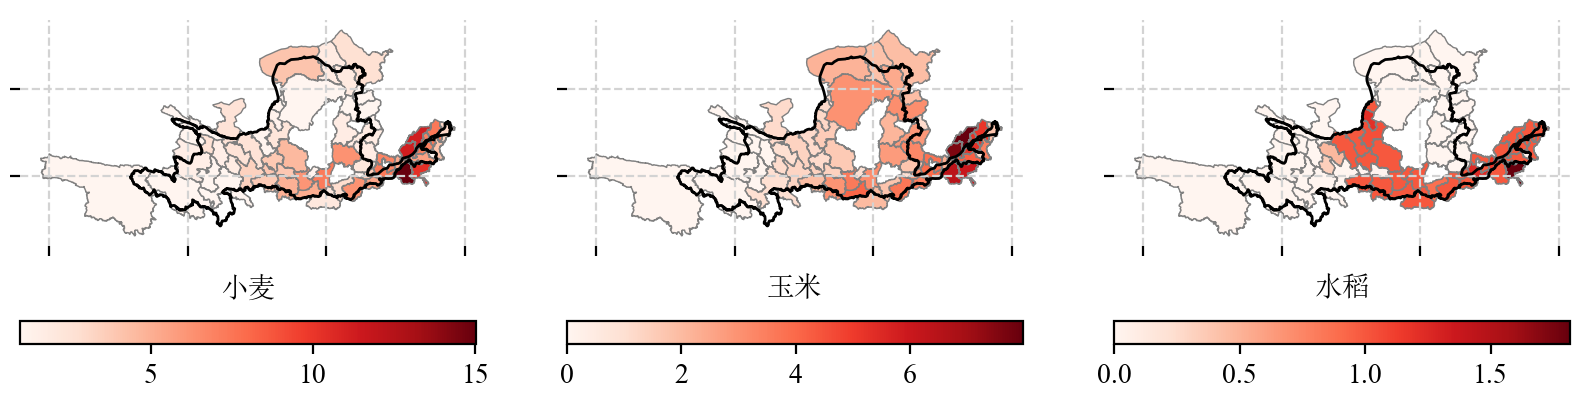
\includegraphics[width=\textwidth]{img/ch6/ch6_agents.png}
%     \caption{黄河流域三种主要粮食作物的平均灌溉主体数量分布}\label{ch6:fig:agents}
% \end{figure}

% \begin{figure}[!ht]
%     \centering
%     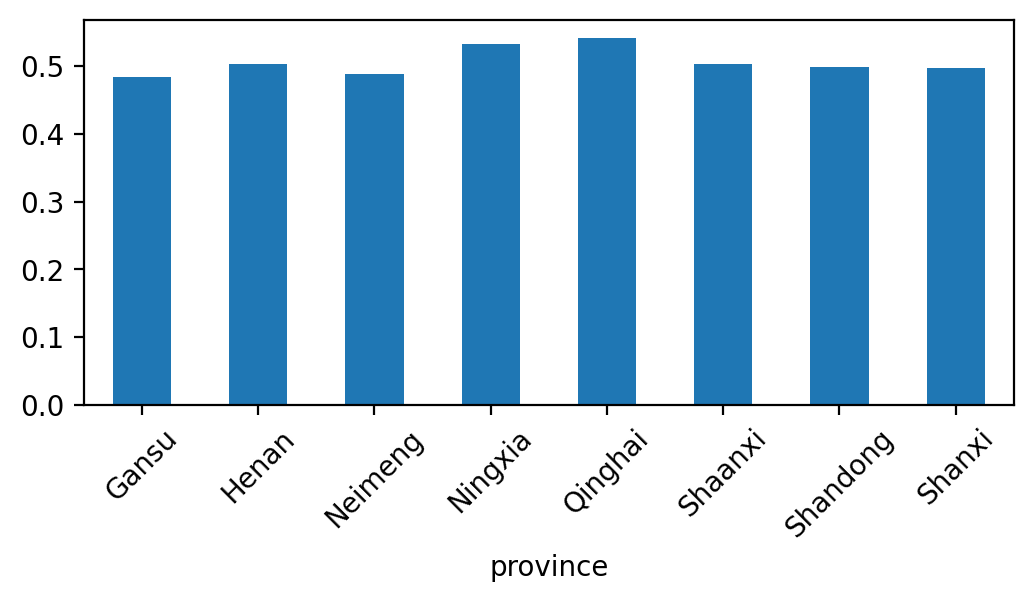
\includegraphics[width=\textwidth]{img/ch6/ch6_compliance.png}
%     \caption{$1988$年至$1997$年主体博弈决策中选择合作的主体比例}\label{ch6:fig:compliacne}
% \end{figure}

\section{灌溉用水来源对分水制度变化的响应}

本研究所建立的模型可以模拟黄河流域主要粮食作物种植中各类水源(降水、地表水、地下水)的使用情况。
天然降水是黄河流域大多数省份粮食作物生长的主要水源,但在河套灌区的宁夏和内蒙古两自治区,地表水灌溉的占比更大(见图\ref{ch6:fig:sources})。
此外,各省总体上都保持了蓝水使用占比持续下降的趋势,但是对用蓝/绿水比例的影响并不明显,仅青海和山西存在一定程度的突变。
另外,通过分析地表水和地下水的使用量的分布情况,发现地表水使用量前$50\%$的主体在1987年到1987年之间用水量进一步扩大,而另外$50\%$用水量较小的地表水使用量则仍分布在约$100~mm$以下,而地下水和灌溉用水的分布在两次分水制度前后的变化不大(图\ref{ch6:fig:sources_change})。


\begin{figure}[!ht]
    \centering
    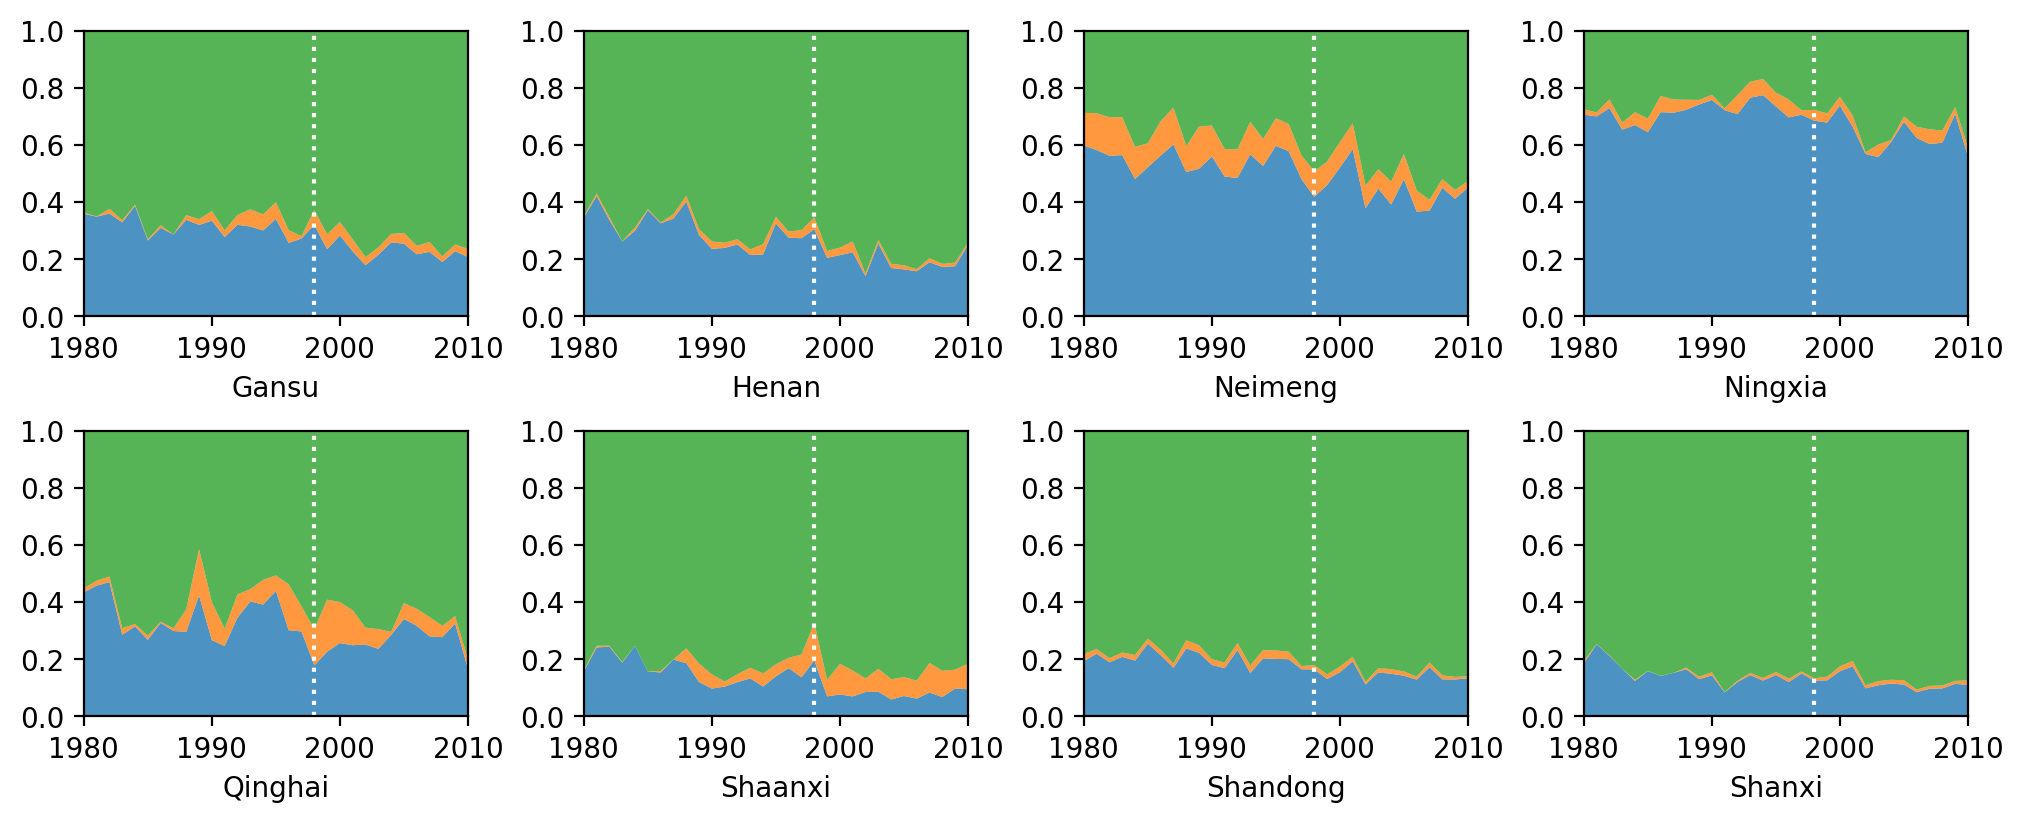
\includegraphics[width=\textwidth]{img/ch6/ch6_green_blue_water.png}
    \caption{黄河流域各省主要粮食作物灌溉用水来源的比例变化}\label{ch6:fig:sources}
\end{figure}

\begin{figure}[!ht]
    \centering
    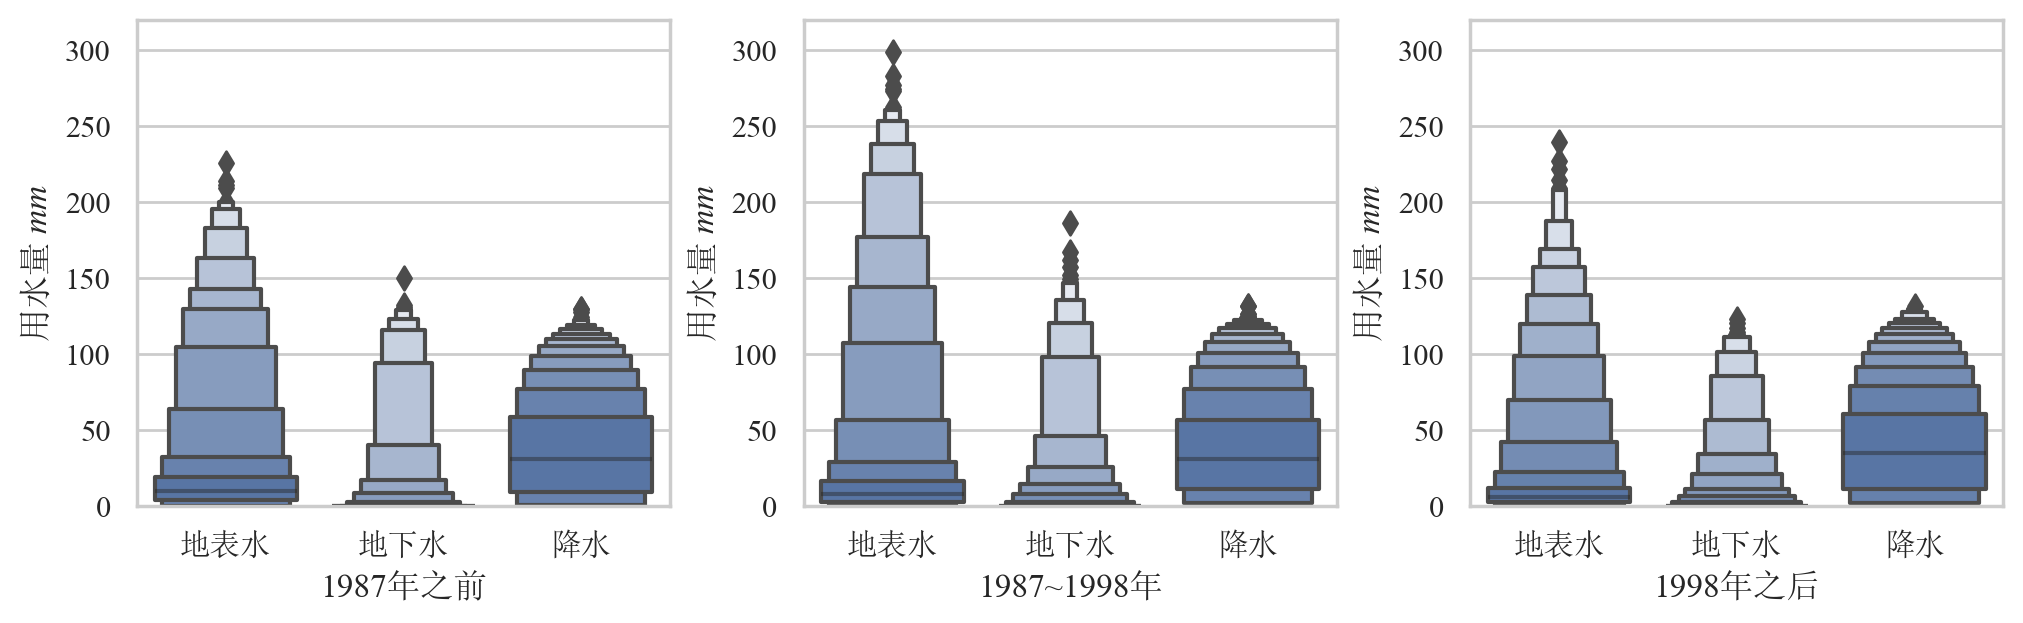
\includegraphics[width=\textwidth]{img/ch6/ch6_sources_change.png}
    \caption{黄河流域分水制度变化前后灌溉用水来源的供水量分布}\label{ch6:fig:sources_change}
\end{figure}

分水制度变化对黄河流域的地下水使用量带来的影响较为明显,且黄河上(头道拐以上)、中(花园口以上)、下游地区对这种变化的响应过程有所差异。
具体来说,下游地区地下水开采量在$1980$年至$2010$年始终维持在较低水平且变化不大;中游地区在此期间则持续增加地下水的开采量;上游在1987年分水制度提出之初期先是增加了地下水开采,在$1991$年左右出现下降趋势(图\ref{ch6:fig:groundwater})。

\begin{figure}[!ht]
    \centering
    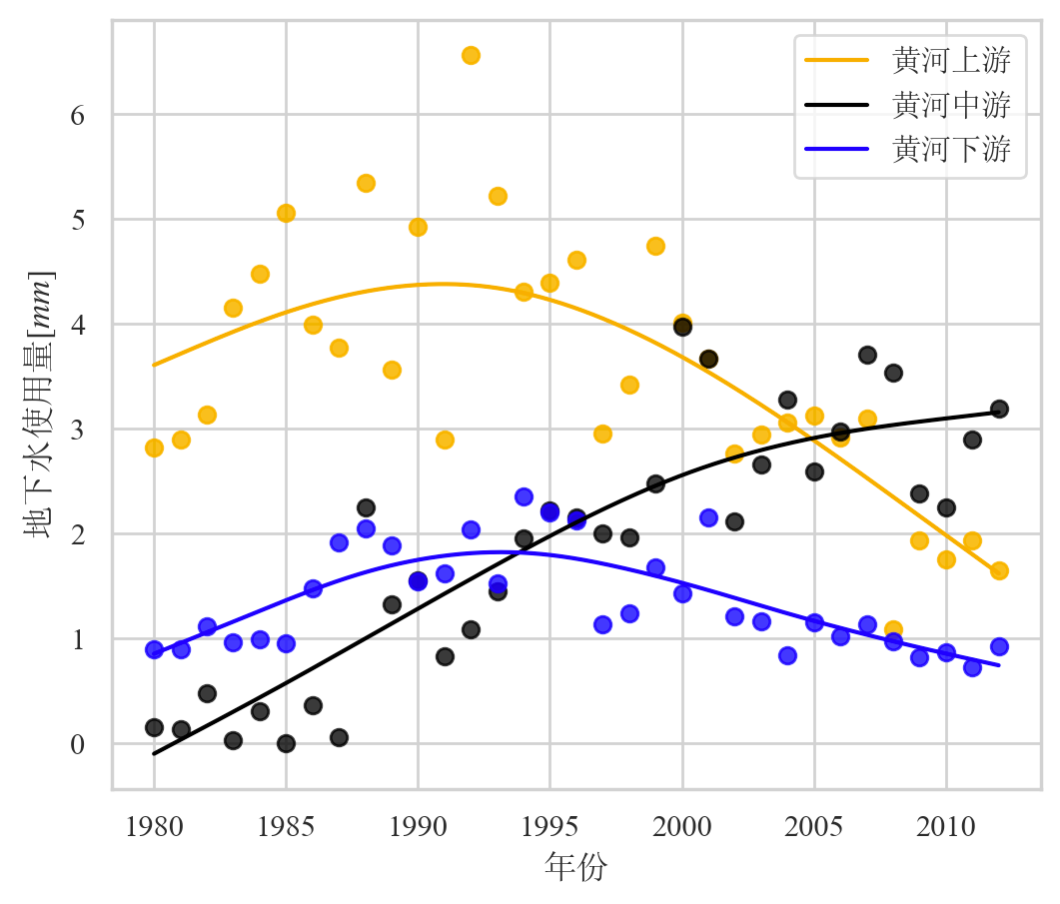
\includegraphics[width=0.6\textwidth]{img/ch6/ch6_groundwater.png}
    \caption{黄河流域不同区域地下水开采量随时间的变化趋势}\label{ch6:fig:groundwater}
\end{figure}

% \section{讨论}\label{ch6:discussion}
\subsection{水资源配额响应错配的原因}

在黄河流域,水资源的配额分配存在一定时空错配的问题,大型灌区是使用水的大户,需要进一步深入研究并制定相应的政策和措施,以保障不同地区的作物水资源供应(图\ref{ch6:fig:matches})。
还需要注意到在不同季节和地区,黄河流域的水资源使用情况存在较大的差异,例如在生长季期间,河套灌区的水资源利用效率偏低,大量的水资源配额供给相对作物实际需求过剩,其他地区则存在供需不平衡的情况。
可能的原因是农业生产需水是在时间和空间上高度集中的,但来自黄河干流的水资源供给需要遵从统一调度,有诸多方面需要协调和权衡,无法优先照顾农业生产的分配,本研究也仅考虑了三种粮食作物的农业灌溉水需求。
此外,偏小的灌溉需求得到的配额也过小,偏大的灌溉需求得到的配额则有所富余,这说明灌溉农业具有引水上的“规模效应”,因此“大引大排”的模式在河套灌区为代表的传统灌溉农业区主导,一些零散分布的灌溉区很难得到如此稳定、集中的配额供给。
正如在本章方法部分中所强调的,本研究在所有需要估计的地方都使用了最优分配的原则,因此实际生产生活中配额与需求的时空错配肯定更为严峻。
这表明在制定水资源管理政策和措施时,需要考虑季节性的变化和区域性的差异,采取针对性的措施,以保障黄河流域的水资源可持续利用和发展。

深入研究分水制度变化对地表水、地下水使用量的影响机制,为制定更有效的水资源管理政策提供科学依据。
在$1980 \sim 2010$三十年间,降水供给的比例持续增加,地表水和地下水同时呈现下降趋势,说明黄河流域各省市的主要粮食作物灌溉在响应分水制度时以节水改革为主,而非简单地用地下水替代被限制的地表水。
河南、山东、宁夏这些黄河用水大省选择遵循配额制度的比例在$10$年后仍显著低于制度颁布之初,这与第五章的数据分析结果相一致,用水大省在$1987$年与$1998$年之间违背配额约束是尚未深入节水改革时,保证农业增长的必然选择。
各省区面对配额制度的不同响应与各地的经济发展本底、地下水资源的分布有关,例如黄河上游的宁蒙灌区则依赖于大引大排,在节水农业推广上多采取鼓励种植节水作物,分水制度颁布初期既超配额采用地表水,又考虑了地下水替代,但在$1998$年后迅速推动节水转型。
中游对配额的遵循程度较好,一定程度上因为难以,因此其地下水抽水量常年稳步提升。
黄河下游因地下水盐碱化问题很难有效利用地下水,经济上的优势使其成为最先推动节水转型的区域,目前节水灌溉率已接近$80\%$。
因此,在制定水资源管理政策和措施时,需要充分考虑不同地区的特点和实际情况,并针对性地制定相应的政策和措施。

\subsection{对黄河流域水资源治理的启示}

黄河流域的水资源分配存在着一定的问题和差异,这对当地的农业生产和经济发展产生了不良影响。
通过分析不同省份的蓝水和绿水使用情况,可以更好地理解不同省份之间的差异和变化,从而制定更好的水资源管理政策和措施。
同时,对于分水制度变化对地下水使用量的影响机制需要进一步深入研究,为制定更有效的水资源管理政策提供科学依据。
综合利用各种水源,提高水资源的利用效率,调整和优化水资源的分配和使用,以满足不同地区的作物生长需求,是保障黄河流域水资源可持续利用的重要措施。

% % 人水匹配 comment mydoc.docx
% 作为实现匹配的一个重要途径,制度分析认为,权利、规则和决策等制度可以引起或解决人与环境互动中的问题。因此,建立匹配的制度可以引导系统功能向理想的结果发展。
% 研究表明,制度匹配在很多方面有利于人类水系统的可持续性。
% 例如,设立流域管理机构可以有效避免水事纠纷,建立水权转换制度有利于资源的有效配置,加强监管可以遏制河流污染。
% 因此,许多大流域的综合治理是建立一套制度的尝试,它以实现人水匹配的一系列制度为核心,包括与之密切相关的文化和技术要素,从而保证流域的可持续发展。
% 这样一个体系的建立庞大而重要,需要自然科学和社会科学的交叉,解耦和理解人水系统中复杂的反馈回路,从而通过制度分析实现人水匹配(图1,PATH 1和路径2)。

% 制度分析往往是在特定背景下进行的,因此,人水关系的动态变化使得宏大的人水系统匹配更加复杂。
% 首先,动态变化是人类社会系统和自然水文系统的共同特征,但只有当关键变量达到临界点时,系统功能的稳态转变才会发生。
% 需要匹配的关键系统功能往往是由流域可持续性的需要决定的,这为理解复杂系统动态的观点提供了价值判断(图1,路径3)。
% 另一方面,当一些可能导致系统稳态转变的变化发生时,也需要重新审视如何在新的人水关系下实现匹配。因此,这些超过阈值的变化可能成为成功过渡到人水匹配的关键驱动力(图1,PATH 4)。
% 然而,实现上述动态匹配还需要对人水系统有更高层次的理解,因为这些动态变化为系统解耦提供了新的科学难题,如变化的弹性、变化之间的因果关系、稳态转化及其级联效应等(图1,PATH 5)。
% 只有通过深度解耦和对反馈循环的理解,才能对人类与水系统的动态进行预测(图1,PATH 6),促进机构分析和过渡匹配(图1,路径1和路径3)。
% 一般来说,人-水系统的反馈循环和动态变化是人-水匹配的基础。由于三者是相互联系的,面对不断变化的流域系统,人水匹配需要动态实现。

\section{小结}\label{ch6:summary}
本章结合包括了三种主要粮食作物(水稻、玉米、小麦)灌溉水需求的自然模块、以及$1987$年“八七”分水制度与$1998$年流域统一调度两次水资源分配制度的人类模块,自下而上构建了黄河流域社会-生态系统的多主体模型。
本章结果指出,黄河流域的水资源分配制度所规定的地表水额度与三种主要粮食作物(水稻、玉米、小麦)的灌溉需求之间存在时空不匹配。
利用模型进一步区分黄河流域历史灌溉用水的来源,发现限制地表取水的水资源分配制度限制并没有直接导致大规模的地下水替代性开采,节水转型是响应制度变化的主要方式。

本章研究表明深入理解人-水关系变化的机制需要考虑人水系统内利益相关者复杂的、差异化的反馈过程。
深入研究分水制度为代表的流域治理措施对流域系统的影响机制,可以为制定更有效的水资源管理政策提供科学依据。

\label{chapter6}

	\chapter{结论与展望}

\section{主要研究结论}

% 研究黄河流域人水关系演变规律、揭示黄河流域人水关系演变机制,有助于深化对人地关系地域系统结构特征和耦合机理的认识,为协调黄河流域人水关系、促进高质量发展提供理论框架和科学依据。
% “人-水关系”是一个尺度敏感的概念,代表了利益相关者与水圈要素过程的联系状态,流域是其理想研究单元,流域系统治理是解析其关系演变机制的重要视角。
本研究以黄河流域为研究区,结合水文气象观测、社会经济统计、历史数据重建、遥感反演等获取多源数据,借助统计分析和模型仿真等手段,解析了黄河流域人水关系的演变过程和驱动机制。
本研究定量揭示了历史时期和现代治黄时期黄河流域人水关系演变过程,分析了不同阶段驱动流域人水关系演变的主要原因。
着眼于对黄河治理转变至关重要的制度驱动力,以水资源配额制度为例,分别从自上而下和自下而上的视角解析了流域人水关系变化的驱动机制,定量评估制度变化产生的影响、发展了流域人水关系演变机制分析的因果推断方法、建立了黄河流域社会-生态系统的多主体模型。
本研究的主要结论如下:

(1)历史时期黄河流域存水沙变化的在两个湿润气候驱动期($900AD\sim1100AD$和$1700AD\sim1900AD$)和两个人类活动驱动期($1350AD \sim 1650AD$ 和 $1900AD$迄今)。其中第一个气候驱动期位于“中世纪暖期”(约$900AD \sim 1100AD$),此时黄河的水沙变化变化仍由气候因素主导。随后中游黄土高原地区发生农田与人口的快速扩张,不断增加的人为压力与另一次潮湿气候共同推动水沙特征在$1700AD \sim 1900AD$越过变化的临界点。上述结果表明人类活动带来的影响最早追溯至$1350AD$才开始取代周期变化的气候,逐步成为历史时期主导黄河流域人-水关系的主要因素。

(2)本研究使用综合水治理指数(IWGI)将当代治黄时期的流域水治理演变过程划分为三个阶段,并依据其各自特点命名为:集中供水时期($1965 \sim 1978$年)、治理转变时期($1979 \sim 2001$年)、以及适应增强时期($2002 \sim 2013$年)。灌区扩张和水库修建的放缓,是黄河从集中供水时期向治理转变时期过渡的主要特征。在治理转变时期流域的非工程治理措施迅速增加,过渡至适应增强时期后保持稳定,并着重提升用水效率。经讨论,上述治理模式转变可能在全世界流域系统中普遍存在,而本研究的分析指出水资源供给趋近极限可能是触发转变的关键。

(3)在上述治理转变期,$1987$年提出的黄河水资源配额制度及其在$1998$年的改革,是对流域影响深远的典型非工程治理政策。本研究指出这两次制度变化以不同的方式重塑了黄河流域的社会-生态系统结构,因而较政策初衷而言产生了不同的治理效果。其中,$1987$年通过的“八七”分水方案违背制度预期地使黄河流域用水量显著增加约$5.75\%$;而$1998$年参照该分水方案施行流域统一调度之后,大多数省份地区的用水量迅速得到控制,流域总用水在接下来十年间以每年$6.6$亿立方米的速度显著下降,成功治理了长达二十余年的黄河断流问题。

(4)黄河水资源配额制度在$1987$年与$1998$年两次变化对流域用水产生的影响,是用水者主体自下而上响应并适应制度变化的表现。本研究耦合了反映水资源配额制度的人类社会模块与计算三种主要粮食作物(水稻、玉米、小麦)灌溉用水需求的自然模块,发展了黄河流域农业灌溉用水者响应分水制度变化的多主体模型。模型仿真结果表明黄河流域的粮食生产灌溉需求与水资源配额之间存在时空不匹配,配额在$1987$至$1998$年间对用水的约束效果不明显,而$1998$年之后,配额制度在约束地表取水的同时也没有导致大规模的地下水开采。

\section{创新点}

(1)本研究定量识别并划分了黄河流域人水关系演变过程的主要阶段,发展了分析其驱动机制的因果推断方法,重点解析了过去常常被忽视的流域非工程治理措施对人水关系演变的驱动作用。

(2)本研究开发了黄河流域社会-生态系统的多主体模型,耦合了水资源分配的社会过程与粮食灌溉需水的自然过程,自下而上解析了农业用水主体对制度变化的响应如何导致不同的流域治理效果。

\section{研究展望}

由于数据来源和研究方法的限制,本论文不可避免地存在一些局限性,可供未来研究做进一步探讨,例如:
(1)第二章的历史时期研究仍无法明确人水关系稳态的弹性范围,需要发展弹性评估方法,建立系统动态模型并量化流域系统的弹性,分析响应洪灾的关系无法继续维系稳态的原因。
(2)第三章开发的综合水治理指数依赖于大量实测和统计数据,因此其应用范围受到数据可获得性的限制。未来可以在全世界流域对子指标进行简化,应用指数构建的框架,分析黄河的人水关系演变过程是否是流域系统的共性规律。
(3)第四章利用社会-生态网络的概念刻画了流域社会-生态系统的结构块,但没能更细致具体地量化其网络结构,未来可利用大数据和网络分析方法量化分析其结构特征,定量推断流域社会-生态系统结构和功能之间的联系。
(4)第五章使用多主体模型探讨了农业用水主体对流域水额分配制度变化的响应,但尚与土壤水、地下水补给、产汇流等水文过程耦合不够紧密。未来可以结合分布式水文模型和系统动力学模型,建立更全面的流域社会-生态系统耦合模型,实现对不同制度情景下黄河流域发展路径的预测。

但本研究以黄河为例在人水关系变化上开展了系统研究,这个典型的人类活动主导的流域凭其复杂的演变过程与演变机制向科学家和决策者证明:流域治理需要深入解析复杂的人-水关系,未来实现人水和谐与流域可持续仍需强调以下三方面:

(1)深化对人水匹配重要性的认识。“流域可持续”的定义是“既满足当代人的需求,又不危及后代满足其需求的能力的发展”,但常常难以准确地了解现在的需求和后代的需要。因此,保证人类系统与水圈的结构匹配非常重要,因为未来的水治理应实现的目标由所有有利益相关者共同决定。

(2)建立观察、解释和预测人与水关系的理论与模型方法。经验观察将指导观测流域系统的哪些变化对治理至关重要,任何解耦和预测流域人-水系统的新理论、新方法,都有利于流域人水关系和谐。本研究表明若不理解复杂的人水关系反馈过程,制度可能带来违背预期的结果,因此需要开发耦合人类社会过程的模型。

(3)评估流域系统人水关系变化对可持续发展的影响。人类世的流域社会-生态环境变化迅速,需要不断调整治理策略进行适应,并在必要时推动治理转型。由于流域治理措施的结果常难以预料,当其呈现出违背预期的表现时,应积极调整对流域治理的治理策略,通过必要的系统转型来促进人水关系和谐。
\label{chapter7}
	
	% 参考文献格式模板文档:https://mirror.las.iastate.edu/tex-archive/biblio/bibtex/contrib/gbt7714/README.md
	% 从 v2.0 版本开始(2020-03-04),用户必须在文档中使用 `\bibliographystyle` 命令选择参考文献样式,
	% 如 `gbt7714-numerical` 或 `gbt7714-author-year`。
	\bibliographystyle{gbt7714-numerical}
	% \bibliographystyle{gbt7714-author-year}
	\bibliography{
	   refs.bib,
	   data/template.bib,
	   chapter1/chapter1.bib,
	   chapter2/chapter2.bib,
	   chapter3/chapter3.bib,
	   chapter4/chapter4.bib,
	   chapter5/chapter5.bib,
	   chapter6/chapter6.bib
   }   
	
   	% 附录
	% \begin{appendix}
	% % !Mode:: "TeX:UTF-8"

\chapter{外文资料原文}
\label{cha:engorg}
As one of the most widely used techniques in operations research, {\em
  mathematical programming} is defined as a means of maximizing a quantity known
as {\em objective function}, subject to a set of constraints represented by
equations and inequalities. Some known subtopics of mathematical programming are
linear programming, nonlinear programming, multiobjective programming, goal
programming, dynamic programming, and multilevel programming$^{[1]}$.

It is impossible to cover in a single chapter every concept of mathematical
programming. This chapter introduces only the basic concepts and techniques of
mathematical programming such that readers gain an understanding of them
throughout the book$^{[2,3]}$.


\section{Single-Objective Programming}
The general form of single-objective programming (SOP) is written
as follows,
\begin{equation}\tag*{(123)} % 如果附录中的公式不想让它出现在公式索引中,那就请
                             % 用 \tag*{xxxx}
\left\{\begin{array}{l}
\max \,\,f(x)\\[0.1 cm]
\mbox{subject to:} \\ [0.1 cm]
\qquad g_j(x)\le 0,\quad j=1,2,\cdots,p
\end{array}\right.
\end{equation}
which maximizes a real-valued function $f$ of
$x=(x_1,x_2,\cdots,x_n)$ subject to a set of constraints.

\newtheorem{mpdef}{Definition}[chapter]
\begin{mpdef}
In SOP, we call $x$ a decision vector, and
$x_1,x_2,\cdots,x_n$ decision variables. The function
$f$ is called the objective function. The set
\begin{equation}\tag*{(456)} % 这里同理,其它不再一一指定。
S=\left\{x\in\Re^n\bigm|g_j(x)\le 0,\,j=1,2,\cdots,p\right\}
\end{equation}
is called the feasible set. An element $x$ in $S$ is called a
feasible solution.
\end{mpdef}

\newtheorem{mpdefop}[mpdef]{Definition}
\begin{mpdefop}
A feasible solution $x^*$ is called the optimal
solution of SOP if and only if
\begin{equation}
f(x^*)\ge f(x)
\end{equation}
for any feasible solution $x$.
\end{mpdefop}

One of the outstanding contributions to mathematical programming was known as
the Kuhn-Tucker conditions\ref{eq:ktc}. In order to introduce them, let us give
some definitions. An inequality constraint $g_j(x)\le 0$ is said to be active at
a point $x^*$ if $g_j(x^*)=0$. A point $x^*$ satisfying $g_j(x^*)\le 0$ is said
to be regular if the gradient vectors $\nabla g_j(x)$ of all active constraints
are linearly independent.

Let $x^*$ be a regular point of the constraints of SOP and assume that all the
functions $f(x)$ and $g_j(x),j=1,2,\cdots,p$ are differentiable. If $x^*$ is a
local optimal solution, then there exist Lagrange multipliers
$\lambda_j,j=1,2,\cdots,p$ such that the following Kuhn-Tucker conditions hold,
\begin{equation}
\label{eq:ktc}
\left\{\begin{array}{l}
    \nabla f(x^*)-\sum\limits_{j=1}^p\lambda_j\nabla g_j(x^*)=0\\[0.3cm]
    \lambda_jg_j(x^*)=0,\quad j=1,2,\cdots,p\\[0.2cm]
    \lambda_j\ge 0,\quad j=1,2,\cdots,p.
\end{array}\right.
\end{equation}
If all the functions $f(x)$ and $g_j(x),j=1,2,\cdots,p$ are convex and
differentiable, and the point $x^*$ satisfies the Kuhn-Tucker conditions
(\ref{eq:ktc}), then it has been proved that the point $x^*$ is a global optimal
solution of SOP.

\subsection{Linear Programming} 
\label{sec:lp}

If the functions $f(x),g_j(x),j=1,2,\cdots,p$ are all linear, then SOP is called
a {\em linear programming}.

The feasible set of linear is always convex. A point $x$ is called an extreme
point of convex set $S$ if $x\in S$ and $x$ cannot be expressed as a convex
combination of two points in $S$. It has been shown that the optimal solution to
linear programming corresponds to an extreme point of its feasible set provided
that the feasible set $S$ is bounded. This fact is the basis of the {\em simplex
  algorithm} which was developed by Dantzig as a very efficient method for
solving linear programming.
\begin{table}[ht]
\centering
  \centering
  \caption*{Table~1\hskip1em This is an example for manually numbered table, which would not appear in the list of tables}
  \label{tab:badtabular2}
  \begin{tabular}[c]{|c|m{0.8in}|c|c|c|c|c|}\hline
    \multicolumn{2}{|c|}{Network Topology} & \# of nodes & 
    \multicolumn{3}{c|}{\# of clients} & Server \\\hline
    GT-ITM & Waxman Transit-Stub & 600 &
    \multirow{2}{2em}{2\%}& 
    \multirow{2}{2em}{10\%}& 
    \multirow{2}{2em}{50\%}& 
    \multirow{2}{1.2in}{Max. Connectivity}\\\cline{1-3}
    \multicolumn{2}{|c|}{Inet-2.1} & 6000 & & & &\\\hline
    \multirow{2}{1in}{Xue} & Rui  & Ni &\multicolumn{4}{c|}{\multirow{2}*{\bnuthesis}}\\\cline{2-3}
    & \multicolumn{2}{c|}{ABCDEF} &\multicolumn{4}{c|}{} \\\hline
\end{tabular}  
\end{table}

Roughly speaking, the simplex algorithm examines only the extreme points of the
feasible set, rather than all feasible points. At first, the simplex algorithm
selects an extreme point as the initial point. The successive extreme point is
selected so as to improve the objective function value. The procedure is
repeated until no improvement in objective function value can be made. The last
extreme point is the optimal solution.

\subsection{Nonlinear Programming}

If at least one of the functions $f(x),g_j(x),j=1,2,\cdots,p$ is nonlinear, then
SOP is called a {\em nonlinear programming}.

A large number of classical optimization methods have been developed to treat
special-structural nonlinear programming based on the mathematical theory
concerned with analyzing the structure of problems.

Now we consider a nonlinear programming which is confronted solely with
maximizing a real-valued function with domain $\Re^n$.  Whether derivatives are
available or not, the usual strategy is first to select a point in $\Re^n$ which
is thought to be the most likely place where the maximum exists. If there is no
information available on which to base such a selection, a point is chosen at
random. From this first point an attempt is made to construct a sequence of
points, each of which yields an improved objective function value over its
predecessor. The next point to be added to the sequence is chosen by analyzing
the behavior of the function at the previous points. This construction continues
until some termination criterion is met. Methods based upon this strategy are
called {\em ascent methods}, which can be classified as {\em direct methods},
{\em gradient methods}, and {\em Hessian methods} according to the information
about the behavior of objective function $f$. Direct methods require only that
the function can be evaluated at each point. Gradient methods require the
evaluation of first derivatives of $f$. Hessian methods require the evaluation
of second derivatives. In fact, there is no superior method for all
problems. The efficiency of a method is very much dependent upon the objective
function.


\chapter{外文资料的调研阅读报告或书面翻译}
\section{单目标规划}
北冥有鱼,其名为鲲。鲲之大,不知其几千里也。化而为鸟,其名为鹏。鹏之背,不知其几
千里也。怒而飞,其翼若垂天之云。是鸟也,海运则将徙于南冥。南冥者,天池也。 
\begin{equation}\tag*{(123)}
 p(y|\mathbf{x}) = \frac{p(\mathbf{x},y)}{p(\mathbf{x})}=
\frac{p(\mathbf{x}|y)p(y)}{p(\mathbf{x})}
\end{equation}

吾生也有涯,而知也无涯。以有涯随无涯,殆已!已而为知者,殆而已矣!为善无近名,为
恶无近刑,缘督以为经,可以保身,可以全生,可以养亲,可以尽年。

\subsection{线性规划}
庖丁为文惠君解牛,手之所触,肩之所倚,足之所履,膝之所倚,砉然响然,奏刀騞然,莫
不中音,合于桑林之舞,乃中经首之会。
\begin{table}[ht]
\centering
  \caption*{表~1\hskip1em 这是手动编号但不出现在索引中的一个表格例子}
  \label{tab:badtabular3}
  \begin{tabular}[c]{|c|m{0.8in}|c|c|c|c|c|}\hline
    \multicolumn{2}{|c|}{Network Topology} & \# of nodes & 
    \multicolumn{3}{c|}{\# of clients} & Server \\\hline
    GT-ITM & Waxman Transit-Stub & 600 &
    \multirow{2}{2em}{2\%}& 
    \multirow{2}{2em}{10\%}& 
    \multirow{2}{2em}{50\%}& 
    \multirow{2}{1.2in}{Max. Connectivity}\\\cline{1-3}
    \multicolumn{2}{|c|}{Inet-2.1} & 6000 & & & &\\\hline
    \multirow{2}{1in}{Xue} & Rui  & Ni &\multicolumn{4}{c|}{\multirow{2}*{\bnuthesis}}\\\cline{2-3}
    & \multicolumn{2}{c|}{ABCDEF} &\multicolumn{4}{c|}{} \\\hline
\end{tabular}  
\end{table}

\begin{table}[ht]
\centering
  \caption{正常附录表格的例子}
  \label{tab:badtabular3}
  \begin{tabular}[c]{|c|m{0.8in}|c|c|c|c|c|}\hline
    \multicolumn{2}{|c|}{Network Topology} & \# of nodes & 
    \multicolumn{3}{c|}{\# of clients} & Server \\\hline
    GT-ITM & Waxman Transit-Stub & 600 &
    \multirow{2}{2em}{2\%}& 
    \multirow{2}{2em}{10\%}& 
    \multirow{2}{2em}{50\%}& 
    \multirow{2}{1.2in}{Max. Connectivity}\\\cline{1-3}
    \multicolumn{2}{|c|}{Inet-2.1} & 6000 & & & &\\\hline
    \multirow{2}{1in}{Xue} & Rui  & Ni &\multicolumn{4}{c|}{\multirow{2}*{\bnuthesis}}\\\cline{2-3}
    & \multicolumn{2}{c|}{ABCDEF} &\multicolumn{4}{c|}{} \\\hline
\end{tabular}  
\end{table}

文惠君曰:“嘻,善哉!技盖至此乎?”庖丁释刀对曰:“臣之所好者道也,进乎技矣。始臣之
解牛之时,所见无非全牛者;三年之后,未尝见全牛也;方今之时,臣以神遇而不以目视,
官知止而神欲行。依乎天理,批大郤,导大窾,因其固然。技经肯綮之未尝,而况大坬乎!
良庖岁更刀,割也;族庖月更刀,折也;今臣之刀十九年矣,所解数千牛矣,而刀刃若新发
于硎。彼节者有间而刀刃者无厚,以无厚入有间,恢恢乎其于游刃必有余地矣。是以十九年
而刀刃若新发于硎。虽然,每至于族,吾见其难为,怵然为戒,视为止,行为迟,动刀甚微,
謋然已解,如土委地。提刀而立,为之而四顾,为之踌躇满志,善刀而藏之。”

文惠君曰:“善哉!吾闻庖丁之言,得养生焉。”


\subsection{非线性规划}
孔子与柳下季为友,柳下季之弟名曰盗跖。盗跖从卒九千人,横行天下,侵暴诸侯。穴室枢
户,驱人牛马,取人妇女。贪得忘亲,不顾父母兄弟,不祭先祖。所过之邑,大国守城,小
国入保,万民苦之。孔子谓柳下季曰:“夫为人父者,必能诏其子;为人兄者,必能教其弟。
若父不能诏其子,兄不能教其弟,则无贵父子兄弟之亲矣。今先生,世之才士也,弟为盗
跖,为天下害,而弗能教也,丘窃为先生羞之。丘请为先生往说之。”

柳下季曰:“先生言为人父者必能诏其子,为人兄者必能教其弟,若子不听父之诏,弟不受
兄之教,虽今先生之辩,将奈之何哉?且跖之为人也,心如涌泉,意如飘风,强足以距敌,
辩足以饰非。顺其心则喜,逆其心则怒,易辱人以言。先生必无往。”

孔子不听,颜回为驭,子贡为右,往见盗跖。


\chapter{其它附录}
前面两个附录主要是给本科生做例子。其它附录的内容可以放到这里,当然如果你愿意,可
以把这部分也放到独立的文件中,然后将其 \verb|\input| 到主文件中。
	% \end{appendix}
	
	% !Mode:: "TeX:UTF-8"
% chktex-file 8

\begin{paper}
\begin{enumerate}
	\item \textbf{Song, S.}, Wang, S., Wu, X., Huang, Y. \& Fu, B. Decreased virtual water outflows from the Yellow River basin are increasingly critical to China. Hydrology and Earth System Sciences 26, 2035-2044 (2022). % (IF = 6.62) 
	\item \textbf{Song, S.} et al. Sediment transport under increasing anthropogenic stress: Regime shifts within the Yellow River, China. Ambio 49, 2015-2025 (2020). % (IF = 6.94) 
	\item \textbf{Song, S.} et al. Improving representation of collective memory in socio-hydrological models and new insights into flood risk management. J Flood Risk Management 14, (2021). % (IF = 4.01) 
	\item \textbf{Song, S.} et al. The responses of Spinifex littoreus to sand burial on the coastal area of Pingtan Island, Fujian Province, South China. Écoscience 1-10 (2021). % (IF = 1.34) 
	\item Wang, S., \textbf{Song, S.}, Zhang, J., Wu, X. \& Fu, B. Achieving a fit between social and ecological systems in drylands for sustainability. Curr. Opin. Environ. Sustain. 48, 53-58 (2021). % (IF = 7.96) 
	\item \textbf{宋爽}, 王帅, 傅伯杰, 陈海滨, 刘焱序, 赵文武. 社会—生态系统适应性治理研究进展与展望. 地理学报, 74, 2401-2410 (2019). % (IF = 10.14) 
	% 接下来是合著
	\item Wu, X., Fu, B. J., Wang S., \textbf{Song S.}, et al. Decoupling of SDGs followed by re-coupling as sustainable development progresses. Nature Sustainability (2022) doi:10.1038/s41893- 022-00868-x. % (IF = 27.2)
	\item Jiao, C., Wang, S., \textbf{Song, S.}, Fu B., Long-term and Seasonal Variation of Open-surface Water Bodies in the Yellow River Basin during 1990-2020. Hydrological Processes, e14846 (2023).
	\item Chen, P., Wang, S., \textbf{Song, S.}, Wang Y., Wang Y., Gao D., Li Z. Ecological restoration intensifies evapotranspiration in the Kubuqi Desert. Ecological Engineering 175, 106504 (2022). % (IF = 4.37) 
	\item Yao, Y., Fu, B., Liu, Y., Wang, Y., \& \textbf{Song, S.} The contribution of ecosystem restoration to sustainable development goals in Asian drylands: A literature review. Land Degrad Dev ldr.4065 (2021). % (IF = 4.38)
	\item Zhang, M., Wang S., Fu, B.J., Wei, X. H., Wang, C., \textbf{Song, S.} Structure Disentanglement and Effect Analysis of the Arid Riverscape Social-Ecological System Using a Network Approach. Sustainability 11, 5159 (2019). % (IF = 3.89) 
	\item Gao, D. Wang, S. Li, Z.D., Wei. F. L., Chen, P., \textbf{Song, S.}. Threshold of vapour- pressure deficit constraint on light use efficiency varied with soil water content. Ecohydrology (2021) doi:10.1002/eco.2305. % (IF = 3.17) 
	\item Li, Z., Wang, S., \textbf{Song, S.}, Wang, Y. \& Musakwa, W. Detecting land degradation in Southern Africa using Time Series Segment and Residual Trend (TSS-RESTREND). Journal of Arid Environments 184, 104314 (2021). % (IF = 2.76) 
	\item 王奕佳, 刘焱序, \textbf{宋爽}, 姚莹, 傅伯杰. 社区尺度社会\textendash{}生态系统适应途径述评. 地理科学进展, 41, 935-944 (2022). % (IF = 6.05) 
	\item 王奕佳, 刘焱序, \textbf{宋爽}, 傅伯杰. 水—粮食—能源—生态系统关联研究进展. 地球科学进展, 36, 684-693 (2021). % (IF = 6.04) 
	
	% \item Yang Y, Ren T L, Zhang L T, et al. Miniature microphone with silicon-based ferroelectric thin films. Integrated Ferroelectrics, 2003, 52:229-235. (SCI 收录, 检索号:758FZ.)
	% \item 杨轶, 张宁欣, 任天令, 等. 硅基铁电微声学器件中薄膜残余应力的研究. 中国机械工程, 2005, 16(14):1289-1291. (EI 收录, 检索号:0534931 2907.)
	% \item 杨轶, 张宁欣, 任天令, 等. 集成铁电器件中的关键工艺研究. 仪器仪表学报,2003, 24(S4):192-193. (EI 源刊.)
	% \item Yang Y, Ren T L, Zhu Y P, et al. PMUTs for handwriting recognition. Inpress. (已被 Integrated Ferroelectrics 录用. SCI 源刊.)
	% \item Wu X M, Yang Y, Cai J, et al. Measurements of ferroelectric MEMS microphones. Integrated Ferroelectrics, 2005, 69:417-429. (SCI 收录, 检索号:896KM.)
	% \item 贾泽, 杨轶, 陈兢, 等. 用于压电和电容微麦克风的体硅腐蚀相关研究. 压电与声光, 2006, 28(1):117-119. (EI 收录, 检索号:06129773469.)
	% \item 伍晓明, 杨轶, 张宁欣, 等. 基于MEMS技术的集成铁电硅微麦克风. 中国集成电路, 2003, 53:59-61.
\end{enumerate}
\end{paper}

	% !Mode:: "TeX:UTF-8"


\begin{ack}

    转眼间,我研究了五年的人与河。河有四时,有盈亏,有荣枯,亦有喜乐哀愁。河没有名字,我在河中打着水漂,所有想说的话河便替我说了——

    人顺河而下,可期百川入海。
    
    感谢恩师傅伯杰院士,学研若沧茫大海,取扁舟一叶横渡,他是“大渡海”的引路人。傅老师的教诲总是简单直接又具有启发性,帮助我这位五年前还徘徊在海边「面朝西边,指向北方」的少年找到了渡海的起点。感谢王帅教授,他包容着我的自由随性,倾听我的理想主义,给我开卷阅读的空间,给我自主探索的时间。渡海途中,我不止一次想对他说「Oh, captain, my captain」!
    
    感谢武旭同老师,从五年前野外相识起,他见证并影响着我的学术思想之演变,几乎每一篇研究工作我都曾向他请教,并总是能得到极有价值的建议。还要感谢北京师范大学许多优秀的老师们,包括但不限于赵文武老师、刘焱序老师、李琰老师、周沙老师、沈妙根老师、缪驰远老师,感谢你们曾在不同场合对我的研究工作做出的指点和帮助。感谢中山大学一直同我保持联系的杜建会老师和胡亮老师,杜老师的敢想敢做与亮哥的认真严谨,都是我学术路途中后知后觉的宝贵财富。
    
    人沿河而行,可辨成长足迹。
    
    感谢可爱的品言,她是不断让我清醒地认识到“人生不止有一个奖章”的灵魂伴侣,她淬炼我的天真与敏锐,使我的好奇心与求知欲常驻。感谢我博士期间的两位舍友卢文路与骆玉川,与他们同处的日常绝不会有一丝枯燥无趣。感谢王奕佳师妹,从中山大学到北师大,从青藏高原到维也纳,她永远是最值得信赖的的战友。感谢其他同院的挚友们,陈鹏、宋佳熙、张疋亥、冯思远,在学术和生活中他们都是能与之畅所欲言的伙伴。感谢课题组各位同仁,尤其是王亚萍、张皓宇、焦晨泰、叶冲冲、高德新、谭子敏,他们在举不胜举的琐事上提供的帮助与支持,使科研生活的点滴得以汇聚成流。
    
    感谢香港大学的李研师兄,五年来他恰到好处的点拨让本不会编程的我逐步将短板补长。感谢北京大学的王文宇与黄永源,中国人民大学的牛昱尧、张炼、与温慧瑜,同他们在经济、历史、考古、社会学等领域的定期探讨极大地开拓了我的视野。感谢我的桥牌搭档、北京大学的肖逸南,他在许多数学问题上给予了我莫大帮助,对我而言好似数次雪中送炭。感谢所有为我提供过资料、信息、修改意见的老师同学乃至陌生审稿人们,我想对你们付出的答谢已毋需言表——我从来没有忽视过任何有价值的建议。
    
    人溯河回望,可见源头活水。
    
    感谢我的父母,他们一直努力为我营造着独立自主、无忧无虑的学习环境。他们默默操持着我们的家,即便来探望我,也会说着「我们看过北京了,我们看过珠海了,我们回家吧」之类的话,只因不想从学业中分走我太多精力。文章我自甘沦落,不觅封侯但觅诗,也许我永远无法成为一个世俗意义上的成功者,但多亏他们的支持,我才能在自己喜欢的道路上坚定前行,我走过的每一段路,笔下的每一个字符,都饱含他们的理解与厚爱。
    
    感谢互联网世界为我提供过帮助的众多开源社区和开源工具,你们使我能够自由勾勒出脑海里的玉宇琼楼,而不必从「先造一颗轮子」开始。功不唐捐无须先磨细铁杵,我心中本有的针才不会荒芜。工具的快速迭代也督促着我保持终身学习,哪怕世上的一切终将腐朽,拥抱开源的人也不必在一天内吃掉五十罐凤梨罐头。
    
    最后,致敬我的精神导师们——爱德华·威尔逊,段义孚,大卫·爱登堡,你们的作品是指引我前进的光,去追寻那个人与自然和谐共处的世界。你们用一份了不起的优雅,维持住了那个世界的幻觉,尽管那里的一切要么未曾到来,要么已经逝去\ldots
    
    悠悠五载换拙文百页,忽忽万绪聚笔尖一言。读博乃极尽自私之事,沿途固多承善意,然答报时光益疏,纵有穷尽感恩之思,终渺沧海之一粟。未尽之人事,今朝情谊铭心坊,来日重逢待报梅。
\end{ack}


\end{document}
